\documentclass[a4paper]{article}
%% Language and font encodings
\usepackage[english]{babel}
\usepackage[utf8x]{inputenc}
\usepackage[T1]{fontenc}
\usepackage{float}
\usepackage[shortlabels]{enumitem}


%% Sets page size and margins
\usepackage[a4paper,top=3cm,bottom=2cm,left=3cm,right=3cm,marginparwidth=1.75cm]{geometry}
\usepackage{fancyhdr}
\pagestyle{fancy}
%% Useful packages and tikz
\usepackage{pgf,tikz,pgfplots}
\pgfplotsset{compat=1.15}
\usepackage{mathrsfs}
\usetikzlibrary{arrows}
\usetikzlibrary{decorations.markings}
\tikzset{->-/.style={decoration={
  markings,
  mark=at position #1 with {\arrow{>}}},postaction={decorate}}}
\tikzset{-<-/.style={decoration={
  markings,
  mark=at position #1 with {\arrow{<}}},postaction={decorate}}}
\usepackage{amsmath}
\usepackage{amsthm}
\usepackage{amsthm,thmtools,xcolor}
\usepackage{eqnarray}
\usepackage{float}
\usepackage{esint}
\usepackage{wrapfig}
\usepackage{gensymb}
\usepackage{lipsum}
\usepackage{amssymb}
\usepackage{array}
\usepackage{tikz}
\usepackage[colorlinks=true, allcolors=blue]{hyperref}
\usepackage{graphicx}
\usepackage{amsmath}
\usepackage{amssymb}
\usepackage{graphicx}
\usepackage[colorlinks=true, allcolors=blue]{hyperref}
\usepackage{mathtools}


% declare math operator
\DeclareMathOperator{\Id}{Id}
\DeclareMathOperator{\Proj}{Proj}
\DeclareMathOperator{\lcm}{lcm}
\DeclareMathOperator{\sgn}{sgn}
\DeclareMathOperator{\Span}{span}
\DeclareMathOperator{\nullity}{nullity}
\DeclarePairedDelimiter\floor{\lfloor}{\rfloor}
\DeclareMathOperator{\res}{res}
\DeclareMathOperator{\rank}{rank}
\DeclareMathOperator{\Ker}{Ker}
\DeclareMathOperator{\R}{R}
\DeclareMathOperator{\Tr}{Tr}
\DeclareMathOperator{\diag}{diag}
\DeclareMathOperator{\Log}{Log}
\DeclareMathOperator{\sech}{sech}
\DeclareMathOperator{\Var}{Var}



%environments
\newtheorem*{foreword*}{Foreword}
\newtheorem{ans}{Answer}[section]

\definecolor{darkblue}{RGB}{	0, 0, 139}
\newtheoremstyle{new}% <name>
{2pt}% <Space above>
{2pt}% <Space below>
{\color{darkblue}}% Body font
{}% <Indent amount>
{\bfseries\color{black}}% Theorem head font
{:}% <Punctuation after theorem head>
{.5em}% <Space after theorem headi>
{}% <Theorem head spec (can be left empty, meaning `normal')>
\theoremstyle{new}
\newtheorem{qns}{Problem}[section]

\setlength{\parindent}{0cm}

\title{\textbf{Problem Sheet for IB NST Mathematics}}
\author{Tai Yingzhe, Tommy (ytt26)}
\date{}
\begin{document}
\maketitle
\tableofcontents
\newpage
\section{Michaelmas Example Sheet 0}
\begin{qns}[Multivariate Taylor Expansion]
Let $f(x)$ be a function of one variable. Working to $O((\delta x)^3)$, write down the Taylor expansion of $f(x+\delta x)$. Let $g(x,y,z)$ be a function of three variables. Working to $O(\delta x,\delta y,\delta z)$, write down the Taylor expansion of $g(x+\delta x,y+\delta y,z+\delta z)$. Express the latter using vector notation.
\end{qns}
\begin{ans}
$$f(x+\delta x)=f(x)+\frac{df}{dx}\delta x+\frac{1}{2!}\frac{d^2f}{dx^2}(\delta x)^2+\frac{1}{3!}\frac{d^3f}{dx^3}(\delta x)^3+O((\delta x)^4)$$
$$g(\mathbf{r}+\delta\mathbf{r})=g(\mathbf{r})+\boldsymbol{\nabla}g\cdot\delta\mathbf{r}+...=e^{\delta\mathbf{r}\cdot\boldsymbol{\nabla}}g(\mathbf{r})$$
\end{ans}
\begin{qns}[Differentiation of an Integral]\leavevmode
\begin{enumerate}[label=(\alph*)]
\item Let $h$ be a function of one variable. Working from first principles, differentiate with respect to $x$ the function
$$I(x)=\int_a^xh(y)dy$$
where $a$ is a constant.
\item Let $f(x,y)$ be a function of two variables. Working from first principles, differentiate with respect to $x$ the function
$$J(x)=\int_a^xf(x,y)dx$$
\end{enumerate}
\end{qns}
\begin{ans}\leavevmode
\begin{enumerate}[label=(\alph*)]
\item Define $h(y)=\frac{dH}{dy}$, so
$$\frac{dI}{dx}=\lim_{\delta x\rightarrow0}\frac{1}{\delta x}\bigg[\int_a^{x+\delta x}h(y)dy-\int_a^xh(y)dy\bigg]=\lim_{\delta x\rightarrow}\frac{H(x+\delta x)-H(x)}{\delta x}=\frac{dH}{dx}=h(x)$$
\item 
$$\frac{dJ}{dx}=\lim_{\delta x\rightarrow0}\frac{1}{\delta x}\bigg[\int_a^{x+\delta x}f(x+\delta x,y)dy-\int_a^xf(x,y)dy\bigg]=\int_a^x\frac{\partial f}{\partial x}dy+f(x,x)$$
where we added a term $-\int_a^{x+\delta x}f(x,y)dy$ and subtracted it. Identifying terms for $\frac{\partial f}{\partial x}$ as well as using result from the previous part, we obtain our desired result.
\end{enumerate}
\end{ans}
\begin{qns}[Ordinary Differential Equations]
Find functions $y(x)$ which satisfy
$$x^2\frac{d^2y}{dx^2}+3x\frac{dy}{dx}-15y=0$$
\end{qns}
\begin{ans}
We try $y=x^n$, and we get $0=n(n-1)+3n-15=n^2+2n-15$ and hence we get $y=c_1x^{-5}+c_2x^3$.\\[5pt]
To obtain the initial guess for $y$. we either do it by intuition (equidimensional equation), or we could try a substitution such that the following transformation occurs: $x\frac{d}{dx}\rightarrow\frac{d}{dt}$ and $x^2\frac{d^2}{dx^2}\rightarrow\frac{d^2}{dt^2}$. This involves the substitution $x=e^t$. Note that if we have equal roots $\lambda$ for the auxiliary equation, we have the form $y=(A+Bt)e^{\lambda t}=(A+B\ln x)x^\lambda$.
\end{ans}
\newpage
\begin{qns}[Fourier Series]\leavevmode
\begin{enumerate}[label=(\alph*)]
\item  The function $h(x) = x(\pi -x)$ is defined on the interval $0\leq x<\pi$. Sketch the odd $2\pi$-periodic continuation of $h(x)$ over the whole real line. Compute the Fourier (sine) series for $h$ and hence demonstrate that
$$\sum_{n=0}^\infty\frac{(-1)^n}{(2n+1)^3}=\frac{\pi^3}{32}$$
\item  Let $g(x)$ be an even periodic function of $x$ with period $4L$, i.e. $g(-x)=g(x)$ and $g(x+4L)=g(x)$. Given that $g(x)=\frac{x-L}{L}$ for $0\leq x\leq 2L$, sketch $g(x)$ for $-4L\leq x\leq 4L$ and find the Fourier series of $g$.
\end{enumerate}
\end{qns}
\begin{ans}\leavevmode
\begin{enumerate}[label=(\alph*)]
\item $h(x)$ is a quadratic with a maximum at $x=\pi/2$ in the given interval. To construct an odd continuation of $h(x)$, we have $h(x)>0$ for $0\leq x\leq\pi$, then we must have $h(x)<0$ (reflect about the $y=0$ line) for $-\pi<x<0$. Since $h(x)$ is odd, let $h(x)=\sum_{n=1}^\infty b_n\sin(nx)$, then
$$b_n=\frac{2}{\pi}\int_0^\pi h(x)\sin(nx)dx=\frac{2}{\pi}\int_0^\pi x(\pi-x)\sin(nx)dx=\frac{4}{n^3\pi}[1-(-1)^n]$$
where we used integration by parts for the integrands $x\sin(nx)$ and $x^2\sin(nx)$, i.e. $$\int x\sin(nx)dx=-\frac{x}{n}\cos(nx)+\frac{1}{n^2}\sin(nx),\quad\int x^2\sin(nx)dx=-\frac{x^2}{n}\cos(nx)+\frac{2}{n^2}x\sin(nx)+\frac{2}{n^3}\cos(nx)$$ hence $\int_0^\pi x\sin(nx)dx=\frac{\pi}{n}[-1+(-1)^n]$ and $\int_0^\pi x^2\sin(nx)dx=-\frac{\pi^2}{n}[-1+(-1)^n]+\frac{2}{n^2}[-1+(-1)^n]$. We thus have $b_n=0$ for even $n$ and $b_n=\frac{8}{n^3\pi}$ if $n$ is odd. Hence,
$$h(x)=\frac{8}{\pi}\sum_{n=0}^\infty\frac{1}{(2n+1)^3}\sin[(2n+1)x]\implies h(x=0.5\pi)=0.5\pi(\pi-0.5\pi)=\frac{8}{\pi}\sum_{n=0}^\infty\frac{(-1)^n}{(2n+1)^3}$$
The result trivially follows.
\item $g(x)$ is a straight line from $g(x=0)=-1$ to $g(x=2L)=1$. Since $g(x)$ is even, let $g(x)=0.5a_0+\sum_{n=1}^\infty a_n\cos(n\pi x/2L)$ where
$$a_0=\frac{2}{2L}\int_0^{2L}g(x)dx=\frac{1}{L}\int_0^{2L}\frac{x-L}{L}dx=\frac{1}{L}\bigg[\frac{x^2}{2L}-x\bigg]^{2L}_0=0$$
$$a_n=\frac{2}{2L}\int_0^{2L}g(x)\cos\frac{n\pi x}{2L}dx=\frac{1}{L}\int_0^{2L}\frac{x-L}{L}\cos\bigg(\frac{n\pi x}{2L}\bigg)dx=\frac{4}{n^2\pi^2}[(-1)^n-1]$$
where we integrate $x\cos(nx)$ by parts, i.e. $\int_0^\pi x\cos(nx)dx=\frac{1}{n^2}[(-1)^n-1]$, and hence $a_n=0$ for even $n$ and $a_n=\frac{-8}{n^2\pi^2}$ for odd $n$. Hence,
$$g(x)=\frac{8}{\pi^2}\sum_{n=0}^\infty\frac{1}{(2n+1)^2}\cos\bigg(\frac{(2n+1)\pi x}{2L}\bigg)$$
\end{enumerate}
\end{ans}
\newpage
\begin{qns}[Index Notation] Show:
\begin{enumerate}[label=(\alph*)]
\item  For vector components $a_i$, $i=1,2,3$:
$$\sum_{j=1}^3a_j\delta_{ij}=a_i$$
where $\delta_{ij}$ is the Kronecker delta.
\item  For independent variables $q_i$, $i=1,2,3$ 
$$\frac{\partial q_i}{\partial q_j}=\delta_{ij}$$
\end{enumerate}
\end{qns}
\begin{ans}\leavevmode
\begin{enumerate}[label=(\alph*)]
\item  $\sum_{j=1}^3a_j\delta_{ij}=a_i$
\item $\frac{\partial q_i}{\partial q_j}=\delta_{ij}$ from definition of partial derivative.
\end{enumerate}
\end{ans}
\begin{qns}[Index Notation] Show that, if $\mathbf{e_i}\cdot\mathbf{e_j}=\delta_{ij}$ for $i,j=1,2,3$ and $\mathbf{e_1}\times\mathbf{e_2}=\mathbf{e_3}$, then
$$\mathbf{e_2}\times\mathbf{e_3}=\mathbf{e_1}~\text{    and    }\mathbf{e_3}\times\mathbf{e_1}=\mathbf{e_2}$$
\end{qns}
\begin{ans}
$$\mathbf{e_3}\times\mathbf{e_1}=(\mathbf{e_1}\times\mathbf{e_2})\times\mathbf{e_1}=-\mathbf{e_1}\times(\mathbf{e_1}\times\mathbf{e_2})=-(\mathbf{e_1}\cdot\mathbf{e_2})\mathbf{e_1}+(\mathbf{e_1}\cdot\mathbf{e_1})\mathbf{e_2}=\mathbf{e_2}$$
$$\mathbf{e_2}\times\mathbf{e_3}=(\mathbf{e_3}\times\mathbf{e_1})\times\mathbf{e_3}=-\mathbf{e_3}\times(\mathbf{e_3}\times\mathbf{e_1})=-(\mathbf{e_3}\cdot\mathbf{e_1})\mathbf{e_3}+(\mathbf{e_3}\cdot\mathbf{e_2})\mathbf{e_1}=\mathbf{e_1}$$
\end{ans}
\begin{qns}[Symmetrical Functions] Using a coordinate system of your choice, write down an example function possessing each of the following kinds of symmetry:
\begin{enumerate}[label=(\alph*)]
    \item A function of 2 variables which has circular symmetry
    \item A function of 3 variables which is spherically symmetric
    \item A function of 3 variables which has axial symmetry
\end{enumerate}
\end{qns}
\begin{ans}\leavevmode
\begin{enumerate}[label=(\alph*)]
\item  $f(r)=r^2\implies f(x,y)=x^2+y^2$. 
\item  $f(\rho)=\rho^2\implies f(x,y,z)=x^2+y^2+z^2$.
\item $f(x,y,z)=f(-x,-y,z)$. Trivially, $f(x,y,z)=z-x^2-y^2$ has this property.
\end{enumerate}
\end{ans}
\begin{qns}[Vector Calculus Index Notation]
Evaluate $\boldsymbol{\nabla}\cdot\mathbf{r}$ and $\boldsymbol{\nabla}\times\mathbf{r}$, where $\mathbf{r}$ is the position vector.
\end{qns}
\begin{ans}
$$\boldsymbol{\nabla}\cdot\mathbf{r}=\frac{\partial x}{\partial x}+\frac{\partial y}{\partial y}+\frac{\partial z}{\partial z}=3$$
$$\boldsymbol{\nabla}\times\mathbf{r}=\boldsymbol{0}$$
\end{ans}
\newpage
\begin{qns}[Vector Calculus Index Notation]
Show that, if $\mathbf{v}=\boldsymbol{\omega}\times\mathbf{r}$, where $\boldsymbol{\omega}$ is a constant vector and $\mathbf{r}$ is the position vector, then $\boldsymbol{\nabla}\times\mathbf{v}=2\boldsymbol{\omega}$. Comment.
\end{qns}
\begin{ans}
$$\boldsymbol{\nabla}\times\mathbf{v}=\boldsymbol{\nabla}\times\begin{pmatrix}\omega_yz-\omega_zy\\\omega_zx-\omega_xz\\\omega_xy-\omega_yx\\\end{pmatrix}=2\boldsymbol{\omega}$$
$\mathbf{v}$ is like a whirlpool. LHS physically means the vorticity, and this is parallel to the angular velocity vector.
\end{ans}
\begin{qns}[Vector Calculus Index Notation]
Let $\psi(\mathbf{r})$ and $\chi(\mathbf{r})$ be scalar fields, and $\mathbf{u}(\mathbf{r})$ and $\mathbf{v}(\mathbf{r})$ vector fields. Show the
following
\begin{enumerate}[label=(\alph*)]
    \item $\boldsymbol{\nabla}\times\psi\mathbf{v}=\boldsymbol{\nabla}\psi\times\mathbf{v}+\psi\boldsymbol{\nabla}\times\mathbf{v}$
    \item 
    $\boldsymbol{\nabla}\cdot(\mathbf{u}\times\mathbf{v})=\mathbf{v}\cdot(\boldsymbol{\nabla}\times\mathbf{u})-\mathbf{u}\cdot(\boldsymbol{\nabla}\times\mathbf{v})$
    and hence
    $$\boldsymbol{\nabla}\cdot(\boldsymbol{\nabla}\psi\times\boldsymbol{\nabla}\chi)=0$$
\end{enumerate}
\end{qns}
\begin{ans}\leavevmode
\begin{enumerate}[label=(\alph*)]
\item  Using suffix notation,
$$\epsilon_{ijk}\frac{\partial}{\partial x_i}(\psi v_j)\hat{k}=\epsilon_{ijk}\frac{\partial\psi}{\partial x_i}v_j\hat{k}+\epsilon_{ijk}\frac{\partial v_j}{\partial x_i}\psi\hat{k}$$
$$\frac{\partial}{\partial x_k}\epsilon_{ijk}u_iv_j=\epsilon_{ijk}\frac{\partial u_i}{\partial x_k}v_j+\epsilon_{ijk}\frac{\partial v_j}{\partial x_k}u_i=\bigg(\epsilon_{kij}\frac{\partial}{\partial x_k}u_i\bigg)v_j-\bigg(\epsilon_{kji}\frac{\partial}{\partial x_k}v_j\bigg)u_i$$
where $\epsilon_{kji}=-\epsilon_{kij}$.
\item We have $\epsilon_{ijk}\frac{\partial^2\psi}{\partial x_k\partial x_i}\frac{\partial\chi}{\partial x_j}+\epsilon_{ijk}\frac{\partial\psi}{\partial x_i}\frac{\partial^2\chi}{\partial x_k\partial x_j}$. By relabelling the dummy indices, this is equal to
$$\epsilon_{kji}\frac{\partial^2\psi}{\partial x_k\partial x_i}\frac{\partial\chi}{\partial x_j}+\epsilon_{ikj}\frac{\partial\psi}{\partial x_i}\frac{\partial^2\chi}{\partial x_j\partial x_k}$$
but $\epsilon_{ijk}=-\epsilon_{kji}$ and $\epsilon_{ijk}=-\epsilon_{ikj}$. Moreover, assuming the second order partial derivatives are symmetric, then both expressions are equal. For $a=-a$, we must conclude $a=0$ for arbitrary $a$. The result thus follows.
\end{enumerate}
\end{ans}
\newpage
\section{Michaelmas Example Sheet 1}
\subsection*{Vector calculus}
\begin{qns}[Suffix notation]
In the following, the indices $i,j,k,l,m$ take the values 1,2,3 and the summation convention applies. In particular, let $\mathbf{n}$ be a unit vector, i.e. $n_in_i=1$.
\begin{enumerate}[label=(\alph*)]
    \item Simplify the following expressions: $$\delta_{ij}a_j,\quad\delta_{ij}\delta_{jk},\quad\delta_{ij}\delta_{ji},\quad\delta_{ij}n_in_j,\quad\epsilon_{ijk}\delta_{jk},\quad\epsilon_{ijk}\epsilon_{ijl},\quad\epsilon_{ijk}\epsilon_{ikj},\quad\epsilon_{ijk}(\mathbf{a}\times\mathbf{b})_k$$
    \item For each of the following equations, either give the equivalent in vector or matrix notation or explain why the equation is invalid.
    $$x_i=a_ib_kc_k+d_i,\quad x_i=a_jb_i+c_kd_ie_kf_j,\quad u=\epsilon_{jkl}v_kw_lx_j$$
    $$\epsilon_{ijk}x_jy_k\epsilon_{ilm}x_ly_m=\mu,\quad A_{ik}B_{kl}=T_{ik}\delta_{kl},\quad x_k=A_{ki} B_{ji}y_j$$
    \item Write the following equations in suffix notation using the summation convention.
    $$(\mathbf{x}+\mu\mathbf{y})\cdot(\mathbf{x}-\mu\mathbf{y})=\kappa,\quad \mathbf{x}=|\mathbf{a}|^2\mathbf{b}-|\mathbf{b}|^2\mathbf{a},\quad (2\mathbf{x}\times\mathbf{y})\cdot(\mathbf{a}+\mathbf{b})=\lambda$$
    \item Given that $A_{ij}=\epsilon_{ijk}a_k$ $\forall i,j$, show $2a_k=\epsilon_{kij}A_{ij}$ $\forall k$.
    \item Show that $\epsilon_{ijk}s_{ij}=0$ $\forall k$ iff $s_{ij}=s_{ji}$ $\forall i,j$.
    \item Given that $N_{ij}=\delta_{ij}-\epsilon_{ijk}n_k+n_in_j$ and $M_{ij}=\delta_{ij}+\epsilon_{ijk}n_k$, show $N_{ij}M_{jk}=2\delta_{ik}$.
\end{enumerate}
\end{qns}
\begin{ans}\leavevmode
\begin{enumerate}[label=(\alph*)]
    \item 
$\delta_{ij}a_j=a_i$; $\delta_{ij}\delta_{jk}=\delta_{ik}$; $\delta_{ij}\delta_{ji}=\delta_{ii}=3$; $\delta_{ij}n_in_j=n_in_i=1$; $\epsilon_{ijk}\delta_{jk}=0$; $\epsilon_{ijk}\epsilon_{ijl}=\delta_{jj}\delta_{kl}-\delta_{jl}\delta_{kj}=3\delta_{kl}-\delta_{kl}=2\delta_{kl}$; $\epsilon_{ijk}\epsilon_{ikj}=-\epsilon_{ijk}\epsilon_{ijk}=-2\delta_{kk}=-6$; $\epsilon_{ijk}(\mathbf{a}\times\mathbf{b})_k=\epsilon_{kij}\epsilon_{klm}a_lb_m=(\delta_{il}\delta_{jm}-\delta_{im}\delta_{jl})a_lb_m=a_ib_j-a_jb_i$
\item $\mathbf{x}=(\mathbf{b}\cdot\mathbf{c})\mathbf{a}+\mathbf{d}$; equation is invalid since $j$ is not a free index but is not repeated; $\mathbf{u}=\mathbf{w}\cdot(\mathbf{x}\times\mathbf{v})$; $|\mathbf{x}\times\mathbf{y}|^2=\mu$; $AB=T$; $x=AB^Ty$
\item $x_ix_i-\mu^2y_iy_i=\kappa$; $x_i=a_ka_kb_i-b_kb_ka_i$; $2\epsilon_{jki}x_jy_k(a_i+b_i)=\lambda$
\item
$$\epsilon_{kij}A_{ij}=\epsilon_{kij}\epsilon_{ijm}a_m=(\delta_{jj}\delta_{km}-\delta_{jm}\delta_{kj})a_m=3a_k-\delta_{kj}a_j=3a_k-a_k=2a_k$$
Note that $A$ has the form 
$$\begin{pmatrix}0&a_3&-a_2\\-a_3&0&a_1\\a_2&-a_1&0\\\end{pmatrix}$$
So, $\epsilon_{kij}A_{ij}=A_{ij}-A_{ji}=a_k-(-a_k)=2a_k$, as desired.
\item Suppose $s_{ij}=s_{ji}$ is true, then
$$\epsilon_{ijk}s_{ij}=\epsilon_{ijk}s_{ji}=-\epsilon_{ijk}s_{ji}\implies 2\epsilon_{ijk}s_{ij}=0$$
by construction and by relabelling indices. Essentially, the sum of the anti-symmetric tensor multiplied by a symmetric tensor is zero.  Conversely, suppose $\epsilon_{ijk}s_{ij}=0$, then
$$0=\epsilon_{lmk}\epsilon_{ijk}s_{ij}=(\delta_{li}\delta_{mj}-\delta_{lj}\delta_{mi})s_{ij}=s_{lm}-s_{ml}$$
\item From the given form,
$$N_{ij}M_{jk}=(\delta_{ij}-\epsilon_{ijm}n_m+n_in_j)(\delta_{jk}+\epsilon_{jkl}n_l)=\delta_{ik}+(\delta_{ik}\delta_{ml}-\delta_{il}\delta_{mk})n_mn_l+n_in_k=2\delta_{ik}$$
where $\epsilon_{jkl}\delta_{ij}n_l-\epsilon_{ijm}\delta_{jk}n_m=0$.
\end{enumerate} 
\end{ans}
\newpage
\begin{qns}[Divergence theorem]
A fluid flow has constant velocity vector in Cartesian coordinates $\mathbf{v}=(0,0,W)$. Explicitly compute the volume flux of fluid $Q=\int\mathbf{v}\cdot d\mathbf{S}$ flowing across
\begin{itemize}
    \item the open hemispherical surface $r=a$, $z\geq0$
    \item the disc $r\leq a$, $z=0$.
\end{itemize}
Verify the divergence theorem.
\end{qns}
\begin{ans} We evaluate for the different regions separately.
\begin{itemize}
    \item For the open hemispherical surface, we have
    $$Q=\int(0,0,W)\cdot(\sin\theta\cos\phi,\sin\theta\sin\phi,\cos\theta)a^2\sin\theta d\theta d\phi=\frac{1}{2}Wa^2\int\sin2\theta d\theta d\phi=Wa^2\pi$$
    \item For the disc, 
    $$Q=\int (0,0,W)\cdot(0,0,1)rdrd\phi=Wa^2\pi$$
\end{itemize}
Divergence theorem states $\int_V(\boldsymbol{\nabla}\cdot\mathbf{F})dV=\int_\mathbf{S}\mathbf{F}\cdot d\mathbf{S}$ and so consider the entire hemispherical volume as $V$, we have
$$\int_S\mathbf{v}\cdot d\mathbf{S}=Wa^2\pi(1-1)=0$$
but
$$\int (\partial_x,\partial_y,\partial_z)\cdot(0,0,W)dV=0$$
and the Divergence theorem is verified to be true for this problem.
\end{ans}
\begin{qns}[Divergence theorem]
For a surface $S$ enclosing a volume $V$, apply the divergence theorem to $\mathbf{F}=p\mathbf{a}$ where $\mathbf{a}$ is an arbitrary constant vector and $p(r)$ is a scalar field. Show
$$\int_V\boldsymbol{\nabla}p(r)dV=\oint_Sp(r)d\mathbf{S}$$
\end{qns}
\begin{ans}
From Divergence theorem,
$$\oint_Sp\mathbf{a}\cdot d\mathbf{S}=\int_V\boldsymbol{\nabla}\cdot(p\mathbf{a})dV=\int_V\boldsymbol{a}\cdot(\boldsymbol{\nabla}p)dV$$
Since $\mathbf{a}$ is a constant vector, we pull it out of the integral sign. Putting both expressions to one side, so that the other side is zero, we have $$\mathbf{a}\cdot(\int_V\boldsymbol{\nabla}pdV-\int_Sp d\mathbf{S})=0$$
For this to be true, either $\mathbf{a}\perp(\int_V\boldsymbol{\nabla}pdV-\int_SpdS)$ or $\int_V\boldsymbol{\nabla}pdV-\int_SpdS=0$ has to be true. The former is not necessarily true since $\mathbf{a}$ is an arbitrary vector.
\end{ans}
\newpage
\begin{qns}[Stokes' theorem]
A time-independent magnetic field $\mathbf{B}(\mathbf{r})$ is given by
$$\mathbf{B}=\frac{\mu_0I}{2\pi}\frac{\mathbf{e_z}\times\mathbf{r}}{x^2+y^2}$$
where $\mu_0$ is the magnetic permeability and I is a constant. Using Cartesian coordinates, calculate the electric current density $\mathbf{J}$ given by the steady Maxwell equation $\boldsymbol{\nabla}\times\mathbf{B}=\mu_0\mathbf{J}$. Also evaluate $\oint_C\mathbf{B}\cdot d\mathbf{r}$ where $C$ is a circle of radius $a$ in the plane
$z = 0$ and centred on $x = y = 0$. Discuss whether Stokes's theorem applies in this
situation.
\end{qns}
\begin{ans}
From the steady Maxwell equation, we have
$$\mu_0\mathbf{J}=\frac{\mu_0I}{2\pi}\bigg(\boldsymbol{\nabla}\times\frac{(0,0,1)\times(x,y,z)}{x^2+y^2}\bigg)=\frac{\mu_0I}{2\pi}\bigg(\frac{x^2+y^2-x(2x)+x^2+y^2-y(2y)}{(x^2+y^2)^2}\bigg)=0$$
so $\mathbf{J}=\boldsymbol{0}$ $\forall x,y$ that does not include the $z$ axis. Otherwise, the integrand blows up. Essentially, $\mathbf{B}$ is not differentiable along the $z$ axis. Now,
$$\oint_C\mathbf{B}\cdot d\mathbf{r}=\frac{\mu_0I}{2\pi}\int_0^{2\pi}\begin{pmatrix}-a\sin\phi/a^2\\a\cos\phi/a^2\\0\\\end{pmatrix}\cdot\begin{pmatrix}-a\sin\phi\\a\cos\phi\\0\\\end{pmatrix}d\phi=\frac{\mu_0I}{2\pi}2\pi=\mu_0I$$
where $\mathbf{r}=(a\cos\phi,a\sin\phi,0)^T$ along $C$ and so $\frac{d\mathbf{r}}{d\phi}=(-a\sin\phi,a\cos\phi,0)^T$. Stokes' theorem do not apply since $\int_S\boldsymbol{\nabla}\times\mathbf{B}dS=0$ but $\oint_C\mathbf{B}\cdot d\mathbf{r}\neq0$.\\[5pt]
This is because $\mathbf{B}$ is not defined at the origin, i.e. a singularity. The region $S$ is not well-connected due to the presence of this singularity, i.e. $\boldsymbol{\nabla}\times\mathbf{B}\neq0$ everywhere in $S$.  To `avoid' this singularity, we integrate along a circular curve $C_\varepsilon$ of constant arbitrary radius $\varepsilon$ (with opposite fashion). Let the original circle of radius $a$ be $C$, then $C'=C\cup C_\varepsilon$, as well as, two additional lines, say both along $y=0$. This is the keyhole contour.
   \begin{center}
    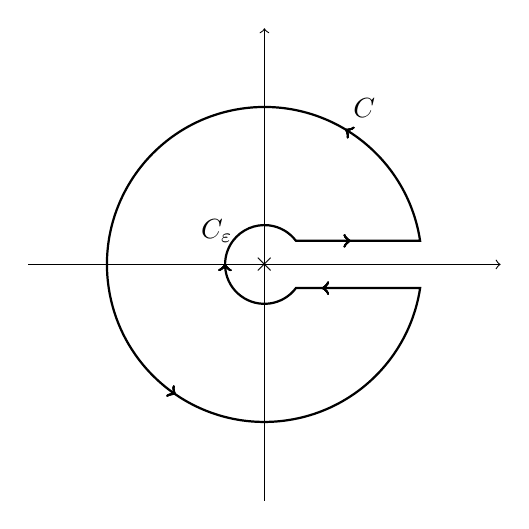
\begin{tikzpicture}
      \draw [->] (-3, 0) -- (3, 0);
      \draw [->] (0, -3) -- (0, 3);

      \draw [black, thick, ->-=0.1, ->-=0.45, ->-=0.75, ->-=0.84, ->-=0.95] (1.977, 0.3) arc(8.63:351.37:2) node [pos=0.15, anchor = south west] {$C$} -- (0.4, -0.3) arc(323.13:36.87:0.5) node [pos=0.7, left] {$C_\varepsilon$} -- cycle;

      \node [circle] at (0, 0) {$\times$};
    \end{tikzpicture}
  \end{center}
We thus have $\int_{C}\mathbf{B}\cdot d\mathbf{r}=-\int_{C_\varepsilon}\mathbf{B}\cdot d\mathbf{r}=-\mu_0I$. This is negative because they traverse in opposite sense. If we sum up, i.e. $\oint_{C'}\mathbf{B}\cdot d\mathbf{r}=0$ as expected. Then, Stokes' theorem do hold in this case, where the new region $S$ does not include $C_\varepsilon$. You may verify that $\varepsilon$ can be arbitrary and the Stokes' theorem still holds.
\end{ans}
\begin{qns}[Laplacian of vector field]
Show in Cartesian coordinates:
$$\nabla^2\mathbf{F}=\boldsymbol{\nabla}(\boldsymbol{\nabla}\cdot\mathbf{F})-\boldsymbol{\nabla}\times(\boldsymbol{\nabla}\times\mathbf{F})$$
This vector identity remains true for all coordinate systems; however, for non-Cartesian coordinates,
$$(\nabla^2\mathbf{F})_i\neq\nabla^2F_i$$
Why is this the case? Illustrate this point by evaluating $\nabla^2\mathbf{F}$ for $\mathbf{F}=f(\rho)\boldsymbol{e_\phi}$ in cylindrical polar coordinates $(\rho,\phi,z)$ and comparing it with $\nabla^2f$.
\end{qns}
\begin{ans} The Laplacian of $\mathbf{F}$ in Cartesian is
$$(\boldsymbol{\nabla}\times(\boldsymbol{\nabla}\times\mathbf{F}))_i=\epsilon_{ijk}\epsilon_{klm}\frac{\partial^2F_m}{\partial x_j\partial x_l}=\frac{\partial^2F_j}{\partial x_i\partial x_j}-\frac{\partial^2F_i}{\partial x_j\partial x_j}=(\boldsymbol{\nabla}(\boldsymbol{\nabla}\cdot\mathbf{F}))_i-(\nabla^2\mathbf{F})_i$$
For $\mathbf{F}=f(\rho)e_\phi$, $\nabla^2\mathbf{F}$ is
$$\boldsymbol{\nabla}\bigg(\frac{1}{\rho}\frac{\partial f}{\partial\phi}\bigg)-\boldsymbol{\nabla}\times\frac{1}{\rho}\bigg(-\mathbf{e_z}\frac{\partial}{\partial z}(\rho f)+\mathbf{e_z}\frac{\partial}{\partial\rho}(\rho f)\bigg)=-\frac{1}{\rho}\bigg[\boldsymbol{e_\rho}\frac{\partial}{\partial\phi}\bigg(\frac{\partial f}{\partial\rho}+\frac{f}{\rho}\bigg)-\rho \boldsymbol{e_\phi}\frac{\partial}{\partial\rho}\bigg(\frac{\partial f}{\partial\rho}+\frac{f}{\rho}\bigg)\bigg]=\boldsymbol{e_\phi}\bigg(\frac{\partial^2f}{\partial\rho^2}+\frac{1}{\rho}\frac{\partial\rho}{\partial\rho}-\frac{f}{\rho^2}\bigg)$$
but $\nabla^2f=\frac{\partial^2f}{\partial\rho^2}+\frac{1}{\rho}\frac{\partial f}{\partial\rho}$, hence result follows. They are not equal since $\mathbf{e_i}$ and $F_i$ are both functions of position.
\end{ans}
\begin{qns}[Biharmonic]
Find the general circularly symmetric solution to
$$\nabla^4\psi:=\nabla^2(\nabla^2\psi)=0$$
Use plane polar coordinates $(\rho,\phi)$. Find those circularly symmetric solutions in the unit disc that are equal to unity at the centre $\rho=0$ and vanish on the boundary $\rho=1$. Give a further condition to render the solution unique.
\end{qns}
\begin{ans}
$\psi$ is independent of $\phi$ since it is circularly symmetric. So, $\psi=\psi(\rho)$
$$\nabla^2f=0\implies \rho\frac{d f}{d\rho}=c_1\implies f=c_1\ln\rho+c_2$$
where $f=\frac{1}{\rho}\frac{\partial}{\partial\rho}(\rho\frac{\partial\psi}{\partial\rho})$. Now evaluating this will be
$$f=\frac{1}{\rho}\frac{d}{d\rho}\bigg(\rho\frac{d\psi}{d\rho}\bigg)=c_1\ln\rho+c_2\implies \psi=c_3\rho^2\ln\rho+c_4\rho^2+c_5\ln\rho+c_6$$
Considering boundary conditions, when $\psi(\rho=0)=1$ would mean $c_5=0$ and $c_6=1$ since $\ln\rho$ not defined at $\rho=0$. $\psi(\rho=1)=0$ would mean $c_4=-1$ and hence $\psi=c_3\rho^2\ln\rho-\rho^2+1$. We need a further condition is needed to render the solution unique, say $\psi(\rho=\rho_0)=C$ for some constant $C$. By the way, $\psi$ is said to be bi-harmonic.
\end{ans}
\begin{qns}[Orthogonal curvilinear coordinates]
Parabolic coordinates $(u,v,\phi)$ are defined in terms of Cartesian coordinates $(x,y,z)$ by
$$x = uv\cos\phi,\quad y = uv\sin\phi ,\quad z =\frac{1}{2}(u^2-v^2)$$
Show that the surfaces of constant $u$, and those of constant $v$, are surfaces obtained by rotating parabolae about the $z$-axis. What are the surfaces of constant $\phi$? Show that the coordinate surfaces intersect at right angles and hence that these coordinates are orthogonal. Find the scale factors $(h_u,h_v,h_\phi)$ defined by
$$|d\mathbf{r}|^2=h_u^2du^2+h_v^2dv^2+h_\phi^2d\phi^2$$
Hence obtain the Laplacian in these coordinates using the formula
$$\nabla^2=\frac{1}{h_1h_2h_3}\bigg[\frac{\partial}{\partial q_1}\bigg(\frac{h_2h_3}{h_1}\frac{\partial}{\partial q_1}\bigg)+\frac{\partial}{\partial q_2}\bigg(\frac{h_3h_1}{h_2}\frac{\partial}{\partial q_2}\bigg)+\frac{\partial}{\partial q_3}\bigg(\frac{h_1h_2}{h_3}\frac{\partial}{\partial q_3}\bigg)\bigg]$$
\end{qns}
\begin{ans}
We have $x^2+y^2=u^2v^2$. For constant $u$, $x^2+y^2=u^4-2u^2z\implies z=\frac{x^2+y^2}{2u^2}-1$ which gives the equation of a paraboloid with rotational symmetry about the $z$ axis, hence the surface of constant $u$ is obtained by rotating a parabola about the $z$ axis. Similarly, for constant $v$, we have $z=\frac{x^2+y^2}{2v^2}+1$, a paraboloid as well. Lastly, we have $y/x=\tan\phi$. So surfaces of constant $\phi$ is a half plane along the line $y=mx$, where $m$ is a constant equal to $\tan\phi$, parallel to the $z$ axis. If $u$ and $v$ are strictly non-negative, the plane is only defined for $x>0$.
\begin{figure}[H]
    \centering
    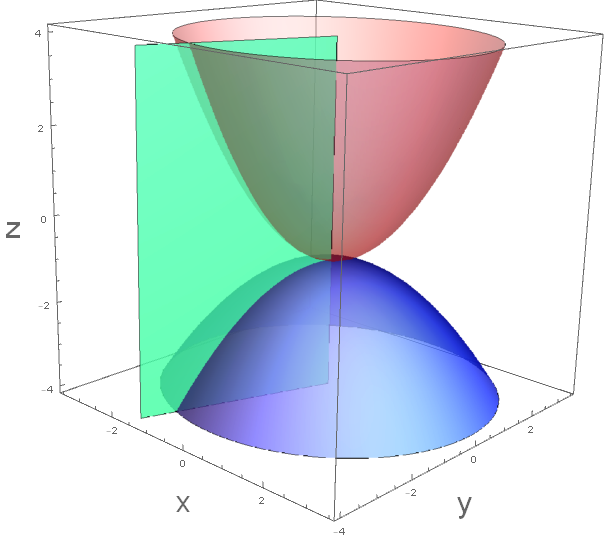
\includegraphics[scale=0.45]{MEx1Q7.png}
    \caption{Three-dimensional Parabolic coordinates: Two confocal paraboloids (blue for constant $u$ and red for constant $v$) and one half-plane. Useful for potential theory of the edges.}
\end{figure}
Moving on, we have $\mathbf{r}=(uv\cos\phi,uv\sin\phi,0.5(u^2-v^2))^T$. So, we have $\mathbf{e_i}=\frac{\partial\mathbf{r}}{\partial i}$ and upon normalizing. 
$$\mathbf{\hat{e}_u}=\frac{1}{\sqrt{v^2+u^2}}\begin{pmatrix}v\cos\phi\\v\sin\phi\\u\\\end{pmatrix}, \quad\mathbf{\hat{e}_v}=\frac{1}{\sqrt{v^2+u^2}}\begin{pmatrix}u\cos\phi\\u\sin\phi\\-v\\\end{pmatrix},\quad\mathbf{\hat{e}_\phi}=\frac{1}{uv}\begin{pmatrix}-uv\sin\phi\\uv\cos\phi\\0\\\end{pmatrix}$$
To show the coordinates are orthogonal, we perform pairwise dot product for $\{\mathbf{\hat{e}_u},\mathbf{\hat{e}_v},\mathbf{\hat{e}_\phi}\}$ and show they each evaluate to zero. Next, we have
$$d\mathbf{r}=\sqrt{v^2+u^2}du\mathbf{\hat{e}_u}+\sqrt{v^2+u^2}dv\mathbf{\hat{e}_v}+uv d\phi\mathbf{\hat{e}_\phi}$$
and so the scale factors are $h_u=\sqrt{u^2+v^2}$ $h_v=\sqrt{u^2+v^2}$ and $h_\phi=uv$. Hence,
\begin{eqnarray}
\nabla^2&=&\frac{1}{uv(u^2+v^2)}\bigg[\frac{\partial}{\partial u}\bigg(uv\frac{\partial}{\partial u}\bigg)+\frac{\partial}{\partial v}\bigg(uv\frac{\partial}{\partial v}\bigg)+\frac{\partial}{\partial\phi}\bigg(\frac{u^2+v^2}{uv}\frac{\partial}{\partial\phi}\bigg)\bigg]\nonumber\\&=&\frac{1}{u(u^2+v^2)}\frac{\partial}{\partial u}+\frac{1}{u^2+v^2}\frac{\partial^2}{\partial u^2}+\frac{1}{v(u^2+v^2)}\frac{\partial}{\partial v}+\frac{1}{u^2+v^2}\frac{\partial^2}{\partial v^2}+\frac{1}{u^2v^2}\frac{\partial^2}{\partial\phi^2}\nonumber
\end{eqnarray}
\end{ans}
\begin{qns}[Orthogonal curvilinear coordinates]
Consider the two-stage transformation of Cartesian coordinates $(x,y,z)$ by
$$x = ax',\quad y=by',\quad z=cz'$$
$$x'=r'\sin\theta'\cos\phi', \quad y'=r'\sin\theta'\sin\phi',\quad z'=r'\cos\theta'$$
where $a,b,c$ are positive constants. Compute the Jacobian matrices of the transformations $(x,y,z)\mapsto(x',y',z')$ and $(x',y',z')\mapsto (r',\theta',\phi')$ and verify explicitly that
$$\frac{\partial(x,y,z)}{\partial(r',\theta',\phi')}=\frac{\partial(x,y,z)}{\partial(x',y',z')}\frac{\partial(x',y',z')}{\partial(r',\theta',\phi')}$$
Are the coordinates $(r',\theta',\phi')$ orthogonal? What range of these coordinates is required to cover the interior of the ellipsoid
$$\frac{x^2}{a^2}+\frac{y^2}{b^2}+\frac{z^2}{c^2}=1$$
Express the volume element in coordinates $(r',\theta',\phi')$ and hence calculate the volume of the ellipsoid.
\end{qns}
\begin{ans}
For $(x,y,z)\mapsto(x',y',z')$, the Jacobian is
$$\frac{\partial(x,y,z)}{\partial(x',y',z')}=\begin{vmatrix}a&0&0\\0&b&0\\0&0&c\\\end{vmatrix}=abc$$
For $(x',y',z')\mapsto(r',\theta',\phi')$, the Jacobian is
$$\frac{\partial(x',y',z')}{\partial(r',\theta',\phi')}=\begin{vmatrix}\sin\theta'\cos\phi'&r'\cos\theta'\cos\phi'&-r'\sin\theta'\sin\phi'\\\sin\theta'\sin\phi'&r'\cos\theta'\sin\phi'&r'\sin\theta'\cos\phi'\\\cos\theta'&-r'\sin\theta'&0\\\end{vmatrix}=r'^2\sin\theta'$$
For $(x,y,z)\mapsto(r',\theta',\phi')$, the Jacobian is
$$\frac{\partial(x,y,z)}{\partial(r',\theta',\phi')}=\begin{vmatrix}a\sin\theta'\cos\phi'&ar'\cos\theta'\cos\phi'&-ar'\sin\theta'\sin\phi'\\b\sin\theta'\sin\phi'&br'\cos\theta'\sin\phi'&br'\sin\theta'\cos\phi'\\c\cos\theta'&-cr'\sin\theta'&0\\\end{vmatrix}=abcr'^2\sin\theta'=\frac{\partial(x,y,z)}{\partial(x',y',z')}\frac{\partial(x',y',z')}{\partial(r',\theta',\phi')}$$
as desired.  In the $(r',\theta',\phi')$ system, we have
$$h_{r'}=\begin{pmatrix}a\sin\theta'\cos\phi'\\b\sin\phi'\sin\theta'\\c\cos\theta'\\\end{pmatrix},\quad h_{\theta'}=\begin{pmatrix}ar'\cos\theta'\cos\phi'\\br'\cos\theta'\sin\phi'\\-r'\sin\theta'\\\end{pmatrix},\quad h_{\phi'}=\begin{pmatrix}-ar'\sin\theta'\sin\phi'\\br'\sin\theta'\cos\phi'\\0\\\end{pmatrix}$$
We can then show that the pairwise dot products of the $h$ vectors are not all zero. Hence, the coordinates $(r',\theta',\phi')$ is not orthogonal.\\[5pt]
For the ellipsoid, we have $r'^2=1$. To cover the interior of the ellipsoid, we require $\{0\leq r'\leq 1, ~0\leq\phi'\leq2\pi,~0\leq \theta'<\pi\}$. The volume element is
$$dV=\bigg|\frac{\partial(x,y,z)}{\partial(r',\theta',\phi')}\bigg|abc dr'd\theta'd\phi'=abcr'^2\sin\theta'dr'd\theta'd\phi'$$
The volume of ellipsoid is 
$$V=abc\int_0^{2\pi}\int_0^\pi\int_0^1r'^2\sin\theta'drd\theta'd\phi'=\frac{4}{3}\pi abc$$
\end{ans}
\begin{qns}[Orthogonal curvilinear coordinates]
In a Cartesian coordinate system $(x_1,x_2,x_3)$, A is the point $(0, 0,-1)$, B is the point
$(0, 0, 1)$ and P is an arbitrary point $(x_1,x_2,x_3)$. In a curvilinear coordinate system, the coordinates of P are specified by
$$u_1=\frac{1}{2}(r_1+r_2),\quad u_2=\frac{1}{2}(r_1-r_2),\quad u_3=\phi$$
where $r_1$ and $r_2$ are the distances AP and BP respectively and $\phi$ is the angle between the planes ABP and $x_2=0$. Show that $x_3=u_1u_2$ and that the distance $\rho$ from P to the $x_3$-axis is equal to $\sqrt{(u_1^2-1)(1-u_2^2)}$. Next, evaluate $\frac{\partial x_i}{\partial u_j}$. Deduce that the curvilinear coordinates are orthogonal and sketch the coordinate surfaces. Show that the metric coefficients are
$$h_1=\sqrt{\frac{u_1^2-u_2^2}{u_1^2-1}},\quad h_2=\sqrt{\frac{u_1^2-u_2^2}{1-u_2^2}},\quad h_3=\sqrt{(u_1^2-1)(1-u_2^2)}$$
Show that if the function $\Psi$ satisfies Laplace's equation and is independent of $u_2$ and $u_3$, then it has the form
$$\Psi=a+b\ln\bigg(\frac{u_1-1}{u_1+1}\bigg)$$
for constant $a$ and $b$.
\end{qns}
\newpage
\begin{ans}
Let the distances from B to P and from A to P be $r_2$ and $r_1$ respectively, then $r_1^2=x_1^2+x_2^2+(x_3+1)^2$ and $r_2^2=x_1^2+x_2^2+(x_3-1)^2$. We then have $u_1u_2=\frac{1}{4}(r_1^2-r_2^2)=x_3$. For the distance from P to the $x_3$ axis is $\rho$,
\begin{eqnarray}
\rho&=&\sqrt{x_1^2+x_2^2}\nonumber\\&=&\sqrt{0.5(x_1^2+x_2^2+(x_3+1)^2)+0.5(x_1^2+x_2^2+(x_3-1)^2)-x_3^2-1}\nonumber\\&=&\sqrt{0.25(r_1+r_2)^2+0.25(r_1-r_2)^2-x_3^2-1}\nonumber\\&=&\sqrt{u_1^2+u_2^2-u_1^2u_2^2-1}\nonumber\\&=&\sqrt{(u_1^2-1)(1-u_2^2)}\nonumber
\end{eqnarray}
Next, we have
$$\mathbf{n_{ABP}}=\begin{pmatrix}-x_1\\-x_2\\1-x_3\\\end{pmatrix}\times\begin{pmatrix}-x_1\\-x_2\\-1-x_3\\\end{pmatrix}=2\begin{pmatrix}x_2\\-x_1\\0\\\end{pmatrix}$$
Since $\phi$ is the angle between the planes ABP and $x_2=0$, then as seen in the horizontal plane $x_3=0$, $\phi$ is the angle between the line OP and the $x_1$ axis, hence $$\cos(u_3)=\frac{(x_2,-x_1,0)\cdot(0,1,0)}{\sqrt{x_1^2+x_2^2}}=\frac{-x_1}{\sqrt{x_1^2+x_2^2}}$$
By geometrical arguments, we have $x_1=\rho\cos(u_3)=\sqrt{(u_1^2-1)(1-u_2^2)}\cos u_3$ and $x_2=\rho\sin(u_3)=\sqrt{(u_1^2-1)(1-u_2^2)}\sin u_3$. Hence, in order to show the coordinate system is orthogonal,
$$\frac{\partial x_1}{\partial u_1}=\frac{u_1-u_1u_2^2}{\sqrt{(u_1^2-1)(1-u_2^2)}}\cos u_3,~\frac{\partial x_1}{\partial u_2}=\frac{u_2-u_1^2u_2}{\sqrt{(u_1^2-1)(1-u_2^2)}}\cos u_3,~\frac{\partial x_1}{\partial u_3}=\sqrt{(u_1^2-1)(1-u_2^2)}\sin u_3$$
$$\frac{\partial x_2}{\partial u_1}=\frac{u_1-u_1u_2^2}{\sqrt{(u_1^2-1)(1-u_2^2)}}\sin u_3,~\frac{\partial x_2}{\partial u_2}=\frac{u_2-u_1^2u_2}{\sqrt{(u_1^2-1)(1-u_2^2)}}\sin u_3,~\frac{\partial x_2}{\partial u_3}=\sqrt{(u_1^2-1)(1-u_2^2)}\cos u_3$$
Moreover, $x_3=u_1u_2$ and so $\frac{\partial x_3}{\partial u_1}=u_2$, $\frac{\partial x_3}{\partial u_2}=u_1$ and $\frac{\partial x_3}{\partial u_3}=0$. The $\mathbf{h}$ vectors will be
$$\mathbf{h_1}=\begin{pmatrix}\frac{u_1-u_1u_2^2}{\sqrt{(u_1^2-1)(1-u_2^2)}}\cos u_3\\\frac{u_1-u_1u_2^2}{\sqrt{(u_1^2-1)(1-u_2^2)}}\sin u_3\\u_2\\\end{pmatrix},\quad\mathbf{h_2}=\begin{pmatrix}\frac{u_2-u_1^2u_2}{\sqrt{(u_1^2-1)(1-u_2^2)}}\cos u_3\\\frac{u_2-u_1^2u_2}{\sqrt{(u_1^2-1)(1-u_2^2)}}\sin u_3\\u_1\\\end{pmatrix},\quad\mathbf{h_3}=\begin{pmatrix}\sqrt{(u_1^2-1)(1-u_2^2)}\sin u_3\\\sqrt{(u_1^2-1)(1-u_2^2)}\cos u_3\\0\\\end{pmatrix}$$
We next do a pairwise dot product for the $\mathbf{h}$ vectors and show that the curvilinear coordinates are indeed orthogonal.\\[5pt]
The coordinate surfaces for $u_3$ are half-planes, where $0<u_3<0.5\pi$ for $x_1>0$, $x_2>0$ and $0.5\pi<u_3<\pi$ for $x_1<0$, $x_2>0$, etc. The coordinate surfaces for $u_1$ are ellipsoids with foci at A and B. The coordinate surfaces for $u_2$ are hyperboloids, with $u_2>0$ represent the branch of the solution above the $x_3=0$ plane, and vice-versa for $u_2<0$. Compare the definitions for $u_1$ and $u_2$ with the conic definitions for ellipses and hyperbolas. (Former being the locus of points such that the sum of distances is a constant; latter being the locus of points such that the difference of distances is a constant.)
\begin{figure}[H]
    \centering
    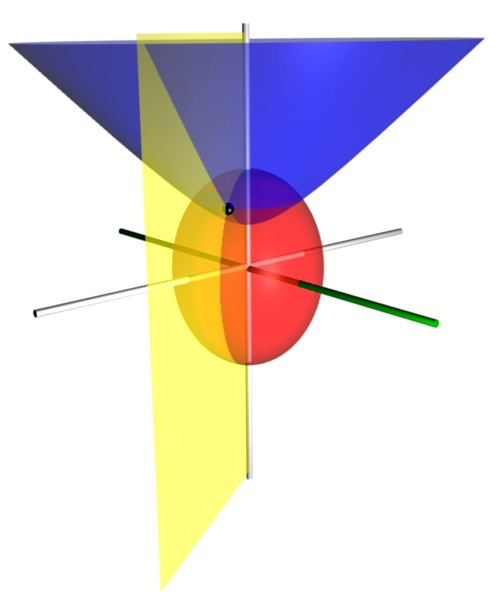
\includegraphics[scale=0.45]{MEx1Q9.png}
    \caption{Prolate Spheroidal Coordinates The red, blue and yellow surfaces are prolate ellipsoid, two-sheet hyperboloid and half-plane. One example is solving for the wavefunction of an electron moving in the electromagnetic field of two positively charged nuclei.}
\end{figure}
The scale factors are trivially computed to be
$$h_1=\sqrt{\frac{u_1^2-u_2^2}{u_1^2-1}},\quad h_2=\sqrt{\frac{u_1^2-u_2^2}{1-u_2^2}},\quad h_3=\sqrt{(u_1^2-1)(1-u_2^2)}$$
hence, the Laplacian will be $\nabla^2\Psi(u_1)=0$. Using the formula from the previous time, we have
$$\frac{\partial}{\partial u_1}\bigg(\frac{h_2h_3}{h_1}\frac{\partial\Psi}{\partial u_1}\bigg)=0\implies\frac{\partial\Psi}{\partial u_1}=\frac{k}{2}\bigg(\frac{1}{u_1-1}-\frac{1}{u_1+1}\bigg)$$
where $\frac{\partial}{\partial u_2}(\frac{h_3h_1}{h_2}\frac{\partial\Psi}{\partial u_2})=0$ and $\frac{\partial}{\partial u_3}(\frac{h_2h_1}{h_3}\frac{\partial\Psi}{\partial u_3})=0$. Trivially, upon integration, we obtain our desired result for $\Psi$, with $b=0.5k$.
$$\Psi=a+b\ln\frac{u_1-1}{u_1+1}$$
\end{ans}
\newpage
\subsection*{Partial differential equations}
\begin{qns}[Wave equation]
A uniform stretched string of length $L$, mass per unit length $\rho$ and tension $T =\rho c^2$ is fixed at both ends. The motion of the string is resisted by the surrounding medium, the resistive force per unit length being $-2\mu\rho\dot{y}$ where $y(x,t)$ is the transverse displacement and $\dot{y}=\frac{\partial y}{\partial t}$. Generalize the argument given in lectures to show that
the equation of motion of the string is
$$\frac{\partial^2y}{\partial t^2}+2\mu\frac{\partial y}{\partial t}=c^2\frac{\partial^2y}{\partial x^2}$$
Find $y(x,t)$ if $\mu=\pi c/L$, $y(x,0)=d\sin(\frac{\pi x}{L})$ and $\dot{y}(x,0)=0$. If an extra transverse force $F\sin(\frac{\pi x}{L})\cos(\pi ct/L)$ per unit length acts on the string, find the resulting forced oscillation.
\end{qns}
\begin{ans}
By Newton's Second Law, we have
$$T\sin(\theta+d\theta)-T\sin\theta-2\mu\rho dx\frac{\partial y}{\partial t}=\rho dx\frac{\partial^2y}{\partial t^2}$$
Using small angle approximations: $\sin\theta\approx\theta$ and $\frac{\partial\theta}{\partial x}\approx\frac{\partial^2y}{\partial x^2}$, we obtain our desired modified wave equation.\\[5pt]
We use separation of variables $y(x,t)=X(x)T(t)$ to get $$\frac{1}{X}\frac{d^2X}{dx^2}=\frac{1}{c^2T}\bigg(\frac{d^2T}{dt^2}+2\mu\frac{dT}{dt}\bigg)=-\lambda^2$$
Since the string is clamped on both ends, the boundary conditions are 
\begin{equation}
    y(0,t)=0,\quad y(L,t)=0\quad \forall t\tag{b.c.s}
\end{equation}
we can deduce 
$$X(x)=c_1\sin(\lambda L)+c_2\cos(\lambda L),\quad\lambda\in\mathbb{Z}$$
Since $T''+2\mu T'+\lambda^2c^2T=0$, we try $T=e^{mt}$ to get the characteristic equation
$$m^2+2\mu m+\lambda^2c^2=0\implies m=-\frac{\pi c}{L}\pm c\sqrt{\frac{\pi^2}{L^2}-\lambda^2}$$
The general solution has the form
$$y(x,t)=(c_1\sin(\lambda L)+c_2\cos(\lambda L))e^{-\pi ct/L}(c_3e^{c\sqrt{(\pi/L)^2-\lambda^2}}+c_4e^{-c\sqrt{(\pi/L)^2-\lambda^2}})$$
which after imposing (b.c.s), $c_2=0$, $\lambda=\frac{n\pi}{L}$ for some $n\in\mathbb{Z}$. Next, we impose the initial conditions. 
\begin{equation}
    y(x,0)=d\sin\frac{\pi x}{L},\quad\dot{y}(x,0)=0\quad \forall t \tag{i.c.s}
\end{equation}
we deduce from $y(x,0)$ that $\lambda=\frac{\pi}{L}$ and $T(0)$ is some constant. But, this $\lambda$ means $m=-\frac{\pi c}{L}$, which gives repeated roots for $e^{mt}$, so $T(t)=(c_3t+c_4)e^{-\pi ct/L}$. At this point, we have 
$$y(x,t)=c_1\sin(\frac{\pi x}{L})(c_3+c_4t)e^{-\pi ct/L}\implies y(x,0)=c_1c_3\sin(\frac{\pi x}{L})\implies  c_1c_3=d$$
Also, 
$$\dot{y}(x,t)=0\implies 0=c_1c_4e^{-\pi ct/L}\sin(\frac{\pi x}{L})-\frac{\pi c}{L}c_1(c_4t+c_3)e^{-\pi ct/L}\sin(\frac{\pi x}{L})\implies c_4=\frac{\pi c}{L}c_3$$
The solution will then be
$$y(x,t)=d\bigg(1+\frac{\pi ct}{L}\bigg)e^{-\pi ct/L}\sin\frac{\pi x}{L}$$
With the extra transverse force, the inhomogeneous PDE is now
$$\frac{\partial^2y}{\partial t^2}+2\mu\frac{\partial y}{\partial t}-c^2\frac{\partial^2y}{\partial x^2}=\frac{F}{\rho}\sin\frac{\pi x}{L}\cos\frac{\pi ct}{L}$$
We first guess a particular solution 
$$y_p=\bigg(A\sin\frac{\pi x}{L}+B\cos\frac{\pi x}{L}\bigg)\bigg(c_1\cos\frac{\pi ct}{L}+c_2\sin\frac{\pi ct}{L}\bigg)$$
Since there is only a single second derivative for $y$ with respect to $x$, $B=0$ (one can show this by assuming first $B\neq0$) and $A$ is absorbed in the arbitrary constants $c_1$ and $c_2$. Now, we evaluate
$$\frac{\partial y_p}{\partial t}=\frac{\pi c}{L}\sin\frac{\pi x}{L}\bigg(-c_1\sin\frac{\pi ct}{L}+c_2\cos\frac{\pi ct}{L}\bigg),~\frac{\partial^2y_p}{\partial t^2}=-\frac{\pi^2c^2}{L^2}y_p,~\frac{\partial^2y_p}{\partial x^2}=-\frac{\pi^2}{L^2}y_p$$
We thus have
$$-\frac{\pi^2c^2}{L^2}y_p+2\frac{\pi c}{L}\frac{\pi c}{L}\sin\frac{\pi x}{L}\bigg(-c_1\sin\frac{\pi ct}{L}+c_2\cos\frac{\pi ct}{L}\bigg)+c^2\frac{\pi^2}{L^2}y_p=\frac{F}{\rho}\sin\frac{\pi x}{L}\cos\frac{\pi ct}{L}$$
and deduce that $c_1=0$, $c_2\frac{2\pi^2c^2}{L^2}=\frac{F}{\rho}\implies c_2=\frac{FL^2}{2\pi^2\rho c^2}$. Hence, the general solution for this inhomogeneous PDE is
$$y(x,t)=y_c+y_p=P\sin\frac{\pi x}{L}(Q+Rt)e^{-\pi ct/L}+\frac{FL^2}{2\pi^2\rho c^2}\sin\frac{\pi x}{L}\sin\frac{\pi ct}{L}$$
where
$$\dot{y}(x,t)=PR\sin\frac{\pi x}{L}e^{-\pi ct/L}-\frac{\pi c}{L}P(Q+Rt)\sin\frac{\pi x}{L}e^{-\pi ct/L}+\frac{FL^2}{2\pi^2\rho c^2}\frac{\pi c}{L}\sin\frac{\pi x}{L}\cos\frac{\pi ct}{L}$$
We need to reobtain the new coefficients $P$, $Q$ and $R$ for the general complementary solution found earlier. This is because of the additional transverse force, and that we have to maintain the same (i.c.s), which after imposing them gives
$$d\sin\frac{\pi x}{L}=y(x,0)=PQ\sin\frac{\pi x}{L}\implies PQ=d$$
$$0=\dot{y}(x,0)=RP\sin(\frac{\pi x}{L})-\frac{\pi c}{L}d\sin(\frac{\pi x}{L})+\frac{FL}{2\rho\pi c}\sin(\frac{\pi x}{L})\implies PR=\frac{\pi cd}{L}-\frac{FL}{2\rho\pi c}$$
Hence, the general solution for this inhomogeneous PDE is
$$y=d\bigg(1+\frac{\pi ct}{L}\bigg)e^{-\pi ct/L}\sin\bigg(\frac{\pi x}{L}\bigg)+\frac{FL^2}{2\pi^2\rho c^2}\bigg[\sin\bigg(\frac{\pi ct}{L}\bigg)-\frac{\pi ct}{L}e^{-\pi ct/L}\bigg]\sin\bigg(\frac{\pi x}{L}\bigg)$$
\end{ans}
\begin{qns}[Laplace's equation]
Show that the solution of Laplace's equation, $\nabla^2\Phi=0$, in the region $0 < x < a$,
$0 < y < b$, $0 < z < c$, with $\Phi= 1$ on the surface $z = 0$ and $\Phi= 0$ on the other surfaces, is
$$\Phi=\frac{16}{\pi^2}\sum_{m=1}^\infty\sum_{n=1}^\infty\frac{\sin[(2m-1)\pi x/a]\sin[(2n-1)\pi y/b]\sinh[k(c-z)]}{(2m-1)(2n-1)\sinh(kc)}$$
where $k^2=\frac{(2m-1)^2\pi^2}{a^2}+\frac{(2n-1)^2\pi^2}{b^2}$. 
\end{qns}
\newpage
\begin{ans}Using separation of variables, $\Phi(x,y,z)=X(x)Y(y)Z(z)$, we have 
$$\frac{1}{X}\frac{d^2X}{dx^2}=-k_1^2,\quad\frac{1}{Y}\frac{d^2Y}{dy^2}=-k_2^2,\quad\frac{1}{Z}\frac{d^2Z}{dz^2}=k_3^2$$
The constants are chosen such that $X$ and $Y$ are sinusoidal while $Z$ is exponential, so as to satisfy the boundary conditions, i.e $k_1>0$, $k_2>0$ and $k_3>0$. The constants also satisfy $k_1^2+k_2^2=k_3^2$.\\[5pt]
Imposing the boundary conditions 
\begin{equation}
    \Phi(0,y,z)=\Phi(a,y,z)=0,\quad \Phi(x,0,z)=\Phi(x,b,z)=0,\quad \Phi(x,y,0)=1,\quad \Phi(x,y,c)=0\tag{b.c.s}
\end{equation}
We then have $k_1=\frac{m\pi}{a}$, $k_2=\frac{n\pi}{b}$, $k_3=\sqrt{\frac{m^2}{a^2}+\frac{n^2}{b^2}}\pi$ $\forall m,n\in\mathbb{Z}^+$. At this point, we have
$$\Phi=\sum_{m=1}^\infty\sum_{n=1}^\infty A_mB_n\sin\frac{m\pi x}{a}\sin\frac{n\pi y}{b}[c_1e^{k_3z}+c_2e^{-k_3z}]$$
which simplifies from $\Phi(x,y,c)=0\implies c_2=-c_1e^{2k_3c}$.
\begin{eqnarray}
Z(z)&=&c_1e^{k_3z}-c_1e^{2k_3c}e^{-k_3z}\nonumber\\&=& c_1[\cosh(k_3z)+\sinh(k_3z)-\cosh(2k_3c-k_3z)-\sinh(2k_3c-k_3z)]\nonumber\\&=&c_1[2\sinh(k_3c)\sinh(k_3c-k_3z)-2\cosh(k_3c)\sinh(k_3(c-z))]\nonumber\\&=&2c_1(\sinh(k_3c)-\cosh(k_3c))\sinh(k_3(c-z))\nonumber
\end{eqnarray}
Let $c_3:=2c_1(\sinh(k_3c)-\cosh(k_3c))$, then solving for the constants using $\Phi(x,y,0)=1$ ,
$$1=\sum_{m=1}^\infty\sum_{n=1}^\infty A_mB_n\sin\frac{m\pi x}{a}\sin\frac{n\pi y}{b}c_3\sinh(k_3c)\implies A_mB_nc_3\sinh(k_3c)=\frac{2}{a}\int_0^a\sin\frac{m\pi x}{a}dx\frac{2}{b}\int_0^b\sin\frac{n\pi x}{b}dx$$
But, $\int_0^a\sin\frac{m\pi x}{a}dx=\frac{2a}{m\pi}$ for odd $m$, and $\int_0^b\sin\frac{n\pi x}{b}dx=\frac{2b}{n\pi}$ for odd $n$. Thus, RHS is $\frac{16}{\pi^2mn}$ for odd $m,n$. The result trivially follows by setting $k_3\rightarrow k$, $m\rightarrow 2m-1$ and $n\rightarrow 2n-1$.
\end{ans}
\begin{qns}[Heat equation]
The temperature distribution $\theta(x,t)$ along a thin bar of length $L$ satisfies the one-dimensional diffusion equation
$$\frac{\partial\theta}{\partial t}=\nu\frac{\partial^2\theta}{\partial x^2}$$
where the diffusivity $\nu$ is a constant, $t$ denotes time and $x$ is the distance from one of the ends. Find $\theta(x,t)$ if the bar is insulated at each end (i.e. if $\frac{\partial\theta}{\partial x}=0$ at each end), and if the initial temperature distribution is given by
$\theta(x,0)=2\theta_0\cos^2(\frac{\pi x}{L})$ where $\theta_0$ is a constant. For large times what is the temperature distribution in the bar? Comment.
\end{qns}
\begin{ans}
Since the boundary conditions are homogeneous, use separation of variables, $\theta(x,t)=X(x)T(t)$, we have $\frac{1}{T}\frac{dT}{dt}=\nu\frac{1}{X}\frac{d^2X}{dx^2}=c$. Set $c=-\nu\lambda^2$. Using a similar approach, we have $\lambda=\frac{n\pi}{L}$ where $n\in\mathbb{Z}^+$, from the boundary conditions  $\frac{\partial\theta}{\partial x}(x=0)=0$ and $\frac{\partial\theta}{\partial x}(x=L)=0$. Hence,
$$\theta(x,t)=\sum_{n=1}^\infty K_n\cos\frac{n\pi x}{L}e^{-\nu n^2\pi^2t/L^2}$$
Impose initial conditions $\theta(x,0)=2\theta_0\cos^2\frac{\pi x}{L}$, we have $\sum_{n=1}^\infty K_n\cos\frac{n\pi x}{L}=2\theta_0\cos^2\frac{\pi x}{L}$. Hence,
$$K_n=\frac{1}{L}\int_0^L\theta_02\cos^2\frac{\pi x}{L}\cos\frac{n\pi x}{L}dx=\frac{2\theta_0}{L}\int_0^L\frac{1}{2}\cos\frac{(n+2)\pi x}{L}+\frac{1}{2}\cos\frac{(n-2)\pi x}{L}+\cos\frac{n\pi x}{L}dx$$
which is $\theta_0$ for $n=0,2$ and zero otherwise. Hence,
$$\theta=\theta_0\bigg(1+\cos\bigg(\frac{2\pi x}{L}\bigg)e^{-4\pi^2\nu t/L^2}\bigg)$$
For large times, $e^{-Ct}\rightarrow 0$, so the temperature distribution becomes uniform at $\theta_0$.
\end{ans}
\newpage
\section{Michaelmas Example Sheet 2}
\subsection*{Green's functions}
\begin{qns}[Dirac Delta]
Define $\delta_\epsilon(x)$ for $\epsilon>0$ by 
$$\delta_\epsilon(x)=
\left\{
        \begin{array}{ll}
      \frac{x+\epsilon}{\epsilon^2} & -\epsilon< x<0 \\
      \frac{\epsilon-x}{\epsilon^2} & 0\leq x<\epsilon\\
      0 & \text{otherwise}
        \end{array}
    \right.$$.
\begin{enumerate}[label=(\alph*)]
    \item Evaluate $\int_{-\infty}^\infty\delta_\epsilon(x)dx$.
    \item Argue that for a good function $f$ and a constant $\xi$,
    $$\lim_{\epsilon\rightarrow0^+}\int_{-\infty}^\infty\delta_\epsilon(x-\xi)f(x)dx=f(\xi)$$
    Hint: Consider the substitution $x-\xi=\epsilon t$
    \item Sketch $\delta_\epsilon(x)$ and comment.
\end{enumerate}
\end{qns}
\begin{ans}\leavevmode
\begin{enumerate}[label=(\alph*)]
\item Evaluate
$$\int_{-\infty}^\infty\delta_\epsilon(x)dx=\int_{-\epsilon}^0\frac{1}{\epsilon^2}(x+\epsilon)dx+\int_0^\epsilon\frac{1}{\epsilon^2}(\epsilon-x)dx=\frac{1}{\epsilon^2}(-0.5\epsilon^2+\epsilon^2)+\frac{1}{\epsilon^2}(\epsilon^2-0.5\epsilon^2)=1$$
\item Using integration by parts,
$$\int_{-\infty}^\infty\delta_\epsilon(x-\xi)f(x)dx=-\int_{-\infty}^\infty\delta_\epsilon'(x-\xi)F(x)dx$$
where $F'(x)=f(x)$. For $\delta_\epsilon'(x-\xi)=\frac{1}{\epsilon^2}$ for $\xi-\epsilon<x<\xi$ and $-\frac{1}{\epsilon^2}$ for $\xi<x<\xi+\epsilon$ and zero otherwise.
$$\int_{-\infty}^\infty\delta_\epsilon(x-\xi)f(x)dx=-\frac{1}{\epsilon^2}\int_{\xi-\epsilon}^\xi F(x)dx+\frac{1}{\epsilon^2}\int_\xi^{\xi+\epsilon}F(x)dx=-\frac{G(\xi)-G(\xi-\epsilon)}{\epsilon^2}+\frac{G(\xi+\epsilon)-G(\xi)}{\epsilon^2}$$
where $G'(x)=F(x)$. Now for the main part, by definition of derivative,
$$\lim_{\epsilon\rightarrow0^+}\int_{-\infty}^\infty\delta_\epsilon(x-\xi)f(x)dx=\lim_{\epsilon\rightarrow0^+}\bigg(-\frac{F(\xi-\epsilon)}{\epsilon}+\frac{F(\xi)}{\epsilon}\bigg)=f(\xi)$$
Alternatively, we use the hint such that
$$\lim_{\epsilon\rightarrow0^+}\int_{-\infty}^\infty\delta_\epsilon(\epsilon t)f(\epsilon t+\xi)d(\epsilon t)=\int_{-\infty}^\infty[\delta_\epsilon(\epsilon t)f(\epsilon t+\xi)]d(\epsilon t)=f(\xi)\int_{-\infty}^\infty\lim_{\epsilon\rightarrow0^+}\bigg[\int_{-\infty}^\infty\delta_\epsilon(\epsilon t)d(\epsilon t)\bigg]=f(\xi)$$
where we used the result for (a) which is true $\forall\epsilon$. The assumption of `good' function comes when we swapped the integrals and the limit operation, since they generally do not commute.
\item The graph will be a triangle, symmetrical about $x=0$ with $\delta_\epsilon(x=0)=1/\epsilon$ and $\delta_\epsilon(x=\pm\epsilon)=0$. $\delta_\epsilon(x)$ is a continuous function but it is not smooth, hence $\delta_\epsilon'(x)$ is discontinuous. As $\epsilon\rightarrow0$, we have an infinite peak at $x=0$.
\begin{center}
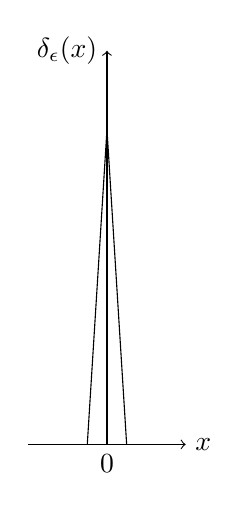
\begin{tikzpicture}
      \draw[->] (-1,0) -- (1,0) node[right] {$x$};
      \draw[->] (0,0) -- (0,5) node[left] {$\delta_\epsilon(x)$};
      \draw[domain=-0.25:0,smooth,variable=\x,black] plot ({\x},{(\x+0.25)/(0.25)^2});
      \draw[domain=0:0.25,smooth,variable=\x,black] plot ({\x},{(-\x+0.25)/(0.25)^2});
      \draw (0,0) node[below]{0};
    \end{tikzpicture}
\end{center}
\end{enumerate}
\end{ans}
\begin{qns}[Dirac Delta]\leavevmode
\begin{enumerate}[label=(\alph*)]
    \item Starting from the definition that $\delta(x)$ is the generalized function such that for all good functions $f(x)$
$$\int_{-\infty}^\infty\delta(x-\xi)f(x)dx=f(\xi)$$
Show that, for constant $a\neq 0$, 
$$\delta(ax)=\frac{1}{|a|}\delta(x)$$
\item  Evaluate 
$$\int_{-\infty}^\infty|x|\delta(x^2-a^2)dx$$
where $a$ is a non-zero constant. Hint: The answer is not $2a$. Consider a substitution such as $t=x^2$ or similar.
\end{enumerate}
\end{qns}
\begin{ans}\leavevmode
\begin{enumerate}[label=(\alph*)]
    \item let $x-\xi=ax'$, we have $\frac{dx}{dx'}=a$. Assume $a$ is positive, $a\int_{-\infty}^\infty\delta(ax')f(\xi+ax')dx'=f(\xi)$ and so $\xi=0$, we have
$$a\int_{-\infty}^\infty\delta(ax')f(ax')dx'=f(0)=\int_{-\infty}^\infty\delta(x')f(x')dx'\implies a\delta(ax')=\delta(x')$$
Similarly, assume $a$ is negative, $a=-|a|$ and so $|a|\delta(ax)=\delta(x)$. Hence, $\forall a$, $\delta(ax)=\frac{1}{|a|}\delta(x)$.
\item let $t=x^2-a^2$, $\frac{dx}{dt}=\frac{1}{2x}$. For positive $x$,
$$\int_0^\infty|x|\delta(x^2-a^2)dx=\int_0^\infty x\delta(x^2-a^2)dx=\frac{1}{2}\int_0^\infty\delta(t-a^2)dt=\frac{1}{2}$$
Similarly, for negative $x$,
$$\int_{-\infty}^0|x|\delta(x^2-a^2)dx=-\int_{-\infty}^0x\delta(t-a^2)dx=\frac{1}{2}\int_0^\infty\delta(t-a^2)dt=\frac{1}{2}$$
Hence, $\int_{-\infty}^\infty|x|\delta(x^2-a^2)dx=1$ if $a\neq 0$. if $a=0$, the integral does not exist because $|x|$ is not differentiable at $x=0$.
\end{enumerate}
\end{ans}
\newpage
\begin{qns}[Motivation for Green's function]
Show that the equation $y"+py'+qy=f(x)$, where $p$ and $q$ are constants, can be written in the form $z'-az=f$ and $y'-by=z$ for suitable choices of the constants $a$ and $b$. Solve these first-order equations using integration factors, subject to the initial conditions $y(0)=y'(0)=0$, to obtain the solution
$$y(x)=e^{bx}\int_0^x\int_0^\eta f(\xi)e^{-a\xi}e^{(a-b)\eta}d\xi d\eta$$
By changing the order of integration and carrying out the integration with respect to $\eta$, show that
$$y(x)=\frac{1}{a-b}\int_0^xf(\xi)[e^{a(x-\xi)}-e^{b(x-\xi)}]d\xi$$
and interpret this result.
\end{qns}
\begin{ans}
$$y''-by'=z'=az+f=a(y'-by)+f\implies y''-(b+a)y'+aby=f$$
We have $-p=b+a$ and $q=ab$, then $q+a^2=-pa$ and hence
$$a=\frac{1}{2}(-p\pm\sqrt{p^2-4q}),~b=\frac{2q}{-p\pm\sqrt{p^2-4q}}$$
For $z'-az=f$, we have the integration factor $e^{-ax}$, then $z=e^{ax}\int_0^xfe^{-ax'}dx'$. Given $y(0)=y'(0)=0$, we have $z(x=0)=0$. So for $y'-by=z$, we use the integration factor $e^{-bx}$,
$$y=e^{bx}\int^x_0ze^{-bx'}dx'=e^{bx}\int^x_0e^{a\eta}e^{-b\eta}\int_0^\eta fe^{-a\xi}d\xi d\eta=e^{bx}\int_0^x\int_0^\eta fe^{(a-b)\eta}e^{-a\xi}d\xi d\eta$$
Now changing the order of integration, $0\leq\xi\leq\eta$ and $0\leq\eta\leq x$ is rewritten as $\xi\leq\eta\leq x$ and $0\leq\xi\leq x$, we then have $y$ being
$$e^{bx}\int_0^x\int_{\xi}^xe^{(a-b)\eta}e^{-a\xi}f(\xi)d\eta d\xi=\frac{1}{a-b}e^{bx}\int_0^x[e^{(a-b)x}-e^{(a-b)\xi}]e^{-a\xi}f(\xi)d\xi=\frac{1}{a-b}\int_0^xf(\xi)[e^{a(x-\xi)}-e^{b(x-\xi)}]d\xi$$
This means that for any second order linear ODE $y"+py'+qy=f$, it is possible to find Green's function
$$G(x,\xi)=\frac{1}{a-b}[e^{a(x-\xi)}-e^{b(x-\xi)}]$$
for $x>\xi$ and 0 for $0\leq x<\xi$, where $-a-b=p$ and $ab=q$. We can then find $y$ using
$$y(x)=\int_0^xf(\xi)G(x,\xi)d\xi$$
\end{ans}
\begin{qns}[Green's function for Heaviside Step]
The differential equation
$$y"+y=H(x)-H(x-\epsilon)$$
where $H$ is the Heaviside step function and $\epsilon>0$ a positive parameter, representing a simple harmonic oscillator subject to a constant force for a finite time. By solving the equation in the three intervals of $x$ separately and applying appropriate matching conditions, show that the solution that vanishes for $x<0$ is
$$y=
\left\{
        \begin{array}{ll}
      0 & x<0 \\
      1-\cos x & 0<x<\epsilon\\
      \cos(x-\epsilon)-\cos x & x>\epsilon
        \end{array}
    \right.$$
Hence show that the solution of $$y"+y=\frac{H(x)-H(x-\epsilon)}{\epsilon}$$
that vanishes for $x<0$ agrees, in the limit $\epsilon\rightarrow 0$, with the appropriate solution of $y"+y=\delta(x)$, namely $y=H(x)\sin(x)$.
\end{qns}
\begin{ans}
We have 
$$y''+y=
\left\{
        \begin{array}{ll}
      1 & 0<x<\epsilon \\
      0& \text{otherwise}
        \end{array}
    \right.$$
The homogeneous solutions are $y_1=\cos(x)$ and $y_2=\sin(x)$. The corresponding Green's function satisfies
$$G''+G=\delta(x-\xi)$$
and from the homogeneous solutions, we have
$$G(x,\xi)=
\left\{
        \begin{array}{ll}
      A(\xi)\cos(x)+B(\xi)\sin(x) & 0\leq x<\xi \\
      C(\xi)\cos(x)+D(\xi)\sin(x)& x>\xi
        \end{array}
    \right.$$
$G$ have to be continuous everywhere, otherwise $G''\propto\delta'(x-\xi)$ which is a contradiction. Integrating over an infinitesimal region $(\xi-\varepsilon,\xi+\varepsilon)$,
$$\lim_{\varepsilon\rightarrow0}\bigg[\int_{\xi-\varepsilon}^{\xi+\varepsilon}G''dx+\int_{\xi-\varepsilon}^{\xi+\varepsilon}Gdx\bigg]=\delta(x-\xi)$$
so the jump condition is $[G']_-^+=1$ at $x=\xi$. The continuity and jump conditions are $x=0$ and $x=\xi$ can be matriculated respectively:
$$\begin{pmatrix}\cos(0)&\sin(0)\\-\sin(0)&\cos(0)\\\end{pmatrix}\begin{pmatrix}A(\xi)\\B(\xi)\\\end{pmatrix}=\begin{pmatrix}0\\0\\\end{pmatrix}\implies A(\xi)=B(\xi)=0$$
$$\begin{pmatrix}\cos(\xi)&\sin(\xi)\\-\sin(\xi)&\cos(\xi)\\\end{pmatrix}\begin{pmatrix}C(\xi)\\D(\xi)\\\end{pmatrix}=\begin{pmatrix}0\\1\\\end{pmatrix}\implies C(\xi)=-\sin(\xi),D(\xi)=\cos(\xi)$$
Hence, 
$$G(x,\xi)=
\left\{
        \begin{array}{ll}
      0 & 0\leq x<\xi \\
      \sin(x-\xi)& x>\xi
        \end{array}
    \right.$$
Solving for $y$, 
$$y(x)=
\left\{
        \begin{array}{ll}
      0 & x<0 \\
      \int_0^x\sin(x-\xi)d\xi=1-\cos x& 0<x<\xi<\epsilon\\
      \int_0^\epsilon\sin(x-\xi)d\xi=\cos(x-\epsilon)-\cos(x)&0<\xi<\epsilon<x
        \end{array}
    \right.$$
Now consider the following DE: $y''+y=\frac{H(x)-H(x-\epsilon)}{\epsilon}$. For $x<0$, $y=0$. For $0<x<\epsilon$, $y=\frac{\cos(0)-\cos(x)}{\epsilon}$. Taking the limit $\epsilon\rightarrow0$, $$y=\lim_{\epsilon\rightarrow0}-\frac{\cos\epsilon-\cos(\epsilon-\epsilon)}{\epsilon}=\lim_{\epsilon\rightarrow0}\frac{d}{d\epsilon}(-\cos\epsilon)=\lim_{\epsilon\rightarrow0}\sin\epsilon=0$$
For $x>\epsilon$, $y=\frac{\cos(x-\epsilon)-\cos(x)}{\epsilon}$, we take the limit $\epsilon\rightarrow0$,
$$y=\lim_{\epsilon\rightarrow0}-\frac{\cos(x)-\cos(x-\epsilon)}{\epsilon}=\lim_{\epsilon\rightarrow0}\frac{d}{d\epsilon}\cos(x-\epsilon)=\sin(x)$$
Hence, $y=H(x)\sin(x)$.
\end{ans}
\newpage
\begin{qns}[Green's Function]
The function $G(x,\xi)$ is defined by
$$G(x,\xi)=
\left\{
        \begin{array}{ll}
      x(\xi-1) & a\leq x\xi \\
      \xi(x-1) & \xi<x\leq 1 
        \end{array}
    \right.$$
If $f(x)$ is continuous for $0\leq x\leq 1$ and 
$$y(x)=\int_0^1f(\xi)G(x,\xi)d\xi$$
Show by direct calculation that $y''(x)=f(x)$ and find $y(0)$ and $y(1)$.\\[5pt] Hint: Use the definition of $G(x,\xi)$ to write $y(x)$ as the sum of two integrals, one with $\xi\leq x$ and the other with $x\leq\xi$.
\end{qns}
\begin{ans} Using the formula for the derivative of $I(\alpha)=\int_{a(\alpha)}^{b(\alpha)}f(x,\alpha)dx$,
$$\frac{dI}{d\alpha}=\int_{a(\alpha)}^{b(\alpha)}\frac{\partial f(x,\alpha)}{\partial\alpha}dx+\frac{db(\alpha)}{d\alpha}f(b,\alpha)-\frac{da(\alpha)}{d\alpha}f(a,\alpha)$$
Consider $y(x)=\int_0^1f(\xi)G(x,\xi)d\xi=\int_0^xf(\xi)\xi(x-1)d\xi+\int_x^1f(\xi)x(\xi-1)d\xi$,
$$y'(x)=\int_0^x\xi   f(\xi)d\xi+x(x-1)f(x)+\int_x^1(\xi-1)f(\xi)d\xi-x(x-1)f(x)=\int_0^x\xi f(\xi)d\xi+\int_x^1(\xi-1)f(\xi)$$
$$y''(x)=xf(x)-(x-1)f(x)=f(x)$$
Lastly, $y(0)=0$ and $y(1)=0$, which must be true by construction.
\end{ans}
\begin{qns}[Green's Function]
Use the method of Green's function to solve
\begin{enumerate}[label=(\alph*)]
    \item $y''-y=x^2$ with $y(0)=y(1)=0$
    \item $y''+\omega^2y=x$ with $y'(0)=y(\pi/\omega)=0$
    \item $y''+\alpha y'=e^{-\beta x}$ with $x\geq0$ and $y(0)=y'(0)=0$
    \item $y^{(4)}=f(x)$ with $y(0)=y'(0)=y''(0)=y^{(3)}(0)=0$.
\end{enumerate}
\end{qns}
\begin{ans}\leavevmode
\begin{enumerate}[label=(\alph*)]
    \item The homogeneous solutions are $e^x$ and $e^{-x}$. The corresponding Green's function satisfy
    $$\frac{\partial^2G(x,\xi)}{\partial x^2}-G(x,\xi)=\delta(x-\xi),\quad G(0,\xi)=G(1,\xi)=0$$
    $G$ must be continuous everywhere otherwise $G''\propto\delta'(x-\xi)$ which is a contradiction. Integrate this over an infinitesimal interval $(\xi-\epsilon,\xi+\epsilon)$ and taking the limit $\epsilon\rightarrow 0$, we then obtain the jump condition at $x=\xi$: $[G']_-^+=1$. At $x\neq\xi$, the Green's function is constructed (in a way that satisfies the b.c.s.) from the linear combination of the linearly independent homogeneous solutions, i.e.
$$G(x,\xi)=
\left\{
        \begin{array}{ll}
      A(\xi)\sinh(x) & 0\leq x<\xi<1 \\
      B(\xi)\sinh(x-1) & 0\leq\xi< x\leq 1 
        \end{array}
    \right.$$
The continuity and jump conditions give
$$\begin{pmatrix}\sinh(\xi)&\sinh(\xi-1)\\\cosh(\xi)&\cosh(\xi-1)\\\end{pmatrix}\begin{pmatrix}-A(\xi)\\B(\xi)\\\end{pmatrix}\begin{pmatrix}0\\1\\\end{pmatrix}\implies\begin{pmatrix}-A(\xi)\\B(\xi)\\\end{pmatrix}=\frac{1}{\sinh(1)}\begin{pmatrix}-\sinh(\xi-1)\\\sinh(\xi)\\\end{pmatrix}$$
The Green's function is then 
$$G(x,\xi)=
\left\{
        \begin{array}{ll}
      \frac{\sinh(\xi-1)}{\sinh(1)}\sinh(x) & 0\leq x<\xi<1 \\
      \frac{\sinh(\xi)}{\sinh(1)}\sinh(x-1) & 0\leq\xi< x\leq 1 
        \end{array}
    \right.$$
The solution to the BVP is then
$$y=\frac{\sinh(x)}{\sinh(1)}\int_x^1\xi^2\sinh(\xi-1)d\xi+\frac{\sinh(x-1)}{\sinh(1)}\int_0^x\xi^2\sinh(\xi)d\xi=\frac{3\sinh(x)-2\sinh(x-1)}{\sinh(1)}-(2+x^2)$$
where we have used the identity $\cosh(x)\sinh(x-1)-\cosh(x-1)\sinh(x)=-\sinh(1)$, as well as $\int x^2\sinh(x)dx=x^2\cosh(x)-2x\sinh(x)+2\cosh(x)$.
\item The homogeneous solutions are $\cos(\omega x)$ and $\sin(\omega x)$. 
The corresponding Green's function satisfy
$$\frac{\partial^2G(x,\xi)}{\partial x^2}+\omega^2G(x,\xi)=\delta(x-\xi),\quad G'(0,\xi)=G(\pi/\omega,\xi)=0$$
Again, $G$ must be continuous everywhere and the jump condition is $[G']_-^+=1$. At $x=\xi$, the Green's function is constructed from the homogeneous solutions
$$G(x,\xi)=
\left\{
        \begin{array}{ll}
      A(\xi)\cos(\omega x) & 0\leq x<\xi\leq\pi/\omega \\
      B(\xi)\sin(\omega x) & 0\leq\xi< x\leq\pi/\omega 
        \end{array}
    \right.$$
Imposing the continuity and jump condition yields:
$$\begin{pmatrix}\cos(\omega\xi)&\sin(\omega\xi)\\-\omega\sin(\omega\xi)&\omega\cos(\omega\xi)\\\end{pmatrix}\begin{pmatrix}-A(\xi)\\B(\xi)\\\end{pmatrix}\begin{pmatrix}0\\1\\\end{pmatrix}\implies\begin{pmatrix}-A(\xi)\\B(\xi)\\\end{pmatrix}=\frac{1}{\omega}\begin{pmatrix}-\sin(\omega\xi)\\\cos(\omega\xi)\\\end{pmatrix}$$
The Green's function will be 
$$G(x,\xi)=
\left\{
        \begin{array}{ll}
      \frac{1}{\omega}\sin(\omega\xi)\cos(\omega x) & 0\leq x<\xi\leq\pi/\omega \\
      \frac{1}{\omega}\cos(\omega\xi)\sin(\omega x) & 0\leq\xi< x\leq\pi/\omega 
        \end{array}
    \right.$$
The solution to the IVP is then
\begin{eqnarray}
y&=&\omega^{-1}\sin(\omega x)\int_0^x\xi\cos(\omega\xi)d\xi+\omega^{-1}\cos(\omega x)\int_x^{\pi/\omega}\xi\sin(\omega \xi)d\xi\nonumber\\&=&\frac{1}{\omega}\sin(\omega x)\bigg(\bigg[\frac{1}{\omega}\xi\sin(\omega\xi)\bigg]^x_0-\int_0^x\frac{1}{\omega}\sin(\omega\xi)d\xi\bigg)+\frac{1}{\omega}\cos(\omega x)\bigg(\bigg[-\frac{1}{\omega}\xi\cos(\omega\xi)\bigg]^{\pi/\omega}_x+\int_x^{\pi/\omega}\frac{1}{\omega}\cos(\omega\xi)d\xi\bigg)\nonumber\\&=&\frac{x}{\omega^2}-\frac{1}{\omega^3}\sin(\omega x)+\frac{\pi}{\omega^3}\cos(\omega x)\nonumber
\end{eqnarray}
\item The homogeneous solutions are $e^{-\alpha x}$ and constant. The corresponding Green's function satisfy
$$\frac{\partial^2G(x,\xi)}{\partial x^2}+\frac{\partial G(x,\xi)}{\partial x}=\delta(x-\xi),\quad G(0,\xi)=G'(0,\xi)=0$$
Again, $G$ is continuous everywhere and $G'$ is continuous everywhere but at $x=\xi$, $[G']_-^+=1$. We guess the Green's function to take the form
$$G(x,\xi)=
\left\{
        \begin{array}{ll}
      A(\xi)e^{-\alpha x}+B(\xi)k & 0\leq x<\xi<\infty \\
      C(\xi)e^{-\alpha x}+D(\xi)k & 0\leq\xi< x\leq \infty
        \end{array}
    \right.$$
where $k$ is a constant. At $x=0$, $[G]_-^+=0$ and $[G']_-^+=0$:
$$\begin{pmatrix}1&k\\-\alpha&0\\\end{pmatrix}\begin{pmatrix}A(\xi)\\B(\xi)\\\end{pmatrix}\begin{pmatrix}0\\0\\\end{pmatrix}\implies\begin{pmatrix}-A(\xi)\\B(\xi)\\\end{pmatrix}=\begin{pmatrix}0\\0\\\end{pmatrix}$$
At $x=\xi$, $[G]_-^+=0$ and $[G']_-^+=1$: 
$$\begin{pmatrix}e^{-\alpha\xi}&k\\-\alpha e^{-\alpha\xi}&0\\\end{pmatrix}\begin{pmatrix}-C(\xi)\\D(\xi)\\\end{pmatrix}\begin{pmatrix}0\\1\\\end{pmatrix}\implies\begin{pmatrix}C(\xi)\\D(\xi)\\\end{pmatrix}=\frac{1}{\alpha ke^{-\alpha\xi}}\begin{pmatrix}-k\\e^{-\alpha\xi}\\\end{pmatrix}$$
The Green's function will be
$$G(x,\xi)=
\left\{
        \begin{array}{ll}
      0 & 0\leq x<\xi<\infty \\
      \frac{1}{\alpha}(1-e^{\alpha(\xi-x)}) & 0\leq\xi< x\leq \infty
        \end{array}
    \right.$$
The solution to the IVP is then
\begin{eqnarray}
y&=&\frac{1}{\alpha}\int_0^xe^{-\beta\xi}d\xi-\frac{1}{\alpha}e^{-\alpha x}\int_0^xe^{(\alpha-\beta)\xi}d\xi\nonumber\\&=&-\frac{1}{\alpha\beta}(e^{-\beta x}-1)-\frac{1}{\alpha(\alpha-\beta)}(e^{-\beta x}-e^{-\alpha x})\nonumber\\&=&\frac{\alpha(1-e^{-\beta x})-\beta(1-e^{-\alpha x})}{\alpha\beta(\alpha-\beta)}\nonumber
\end{eqnarray}
\item The solutions to the homogeneous equation $y^{(4)}=0$ are $x^3$, $x^2$, $x$ and $k$, a constant. The corresponding Green's function satisfy $$G^{(4)}=\delta(x-\xi),\quad G(0,\xi)=G'(0,\xi)=G''(0,\xi)=G^{(3)}(0,\xi)=0$$
$G,G',G''$ must be continuous everywhere otherwise $G^{(4)}\propto\delta'(x-\xi)$ or its higher order derivatives, which is a contradiction. Integrate this over an infinitesimal interval $(\xi-\epsilon,\xi+\epsilon)$ and take the limit $\epsilon\rightarrow 0$ to obtain the jump condition at $x=\xi$: $[G^{(3)}]_-^+=1$. But $G^{(3)}$ is continuous everywhere else. We guess the Green's function to be of the form
$$G(x,\xi)=
\left\{
        \begin{array}{ll}
      A(\xi)x^3+B(\xi)x^2+C(\xi)x+D(\xi)k & 0\leq x<\xi<\infty \\
      P(\xi)x^3+Q(\xi)x^2+R(\xi)x+S(\xi)k & 0\leq\xi< x\leq \infty
        \end{array}
    \right.$$
At $x=0$, $[G]_-^+=[G']_-^+=[G'']_-^+=[G^{(3)}]_-^+=0$, and so $A=B=C=D=0$. But at $x=\xi$, $[G]_-^+=[G']_-^+=[G'']_-^+=0$ and $[G^{(3)}]_-^+=1$ give $$P\xi^3+Q\xi^2+R\xi+Sk=0,\quad 3P\xi^2+2Q\xi+R=0$$ 
$$6P\xi+2Q=0,\quad 6P=1$$
We have $P=\frac{1}{6}$, $Q=-\frac{1}{2}\xi$, $R=\frac{1}{2}\xi^2$, $S=-\frac{1}{6k}\xi^3$. The Green's function is
$$G(x,\xi)=
\left\{
        \begin{array}{ll}
      0& 0\leq x<\xi<\infty \\
      \frac{1}{6}x^3-\frac{1}{2}\xi x^2+\frac{1}{2}\xi^2x-\frac{1}{6}\xi^3 & 0\leq\xi< x\leq \infty
        \end{array}
    \right.$$
The solution to the IVP is then
$$y=\int_0^xf(\xi)\bigg(\frac{1}{6}x^3-\frac{1}{2}\xi x^2+\frac{1}{2}\xi^2x-\frac{1}{6}\xi^3\bigg)d\xi$$
\end{enumerate}
\end{ans}
\newpage
\subsection*{Fourier transform}
\begin{qns}[Fourier transform of even/odd functions]
Let $\alpha$ and $\beta$ be positive constants, and let $H(x)$ denote the Heaviside step function. Find the Fourier transforms of 
\begin{enumerate}[label=(\alph*)]
    \item the odd function $f_o(x)$, where $f_o$ is defined for $x>0$ by 
    $$f_o(x)=
\left\{
        \begin{array}{ll}
      1 & 0< x\leq 1 \\
      0 & x>1 
        \end{array}
    \right.$$
    \item the even function $f_e(x)=e^{-|x|}$.
    \item the even function $g(x)$, where
    $$g(x)=
\left\{
        \begin{array}{ll}
      1 & |x|<\alpha \\
      0 & |x|\geq\alpha 
        \end{array}
    \right.$$
    \item the function
    $$h(x)=H(x)\sinh(\alpha x)e^{-\beta x}$$
    where $\alpha<\beta$.
\end{enumerate}
\end{qns}
\begin{ans}
Note that functions stay odd/even after being Fourier transformed. Moreover, suppose $f(x)=f_e(x)+f_o(x)$ can be written into its odd and even parts, then after integrating over a symmetric interval during the Fourier transform, we have
$$\tilde{f}(k)=\int f_e(x)\cos(kx)dx-i\int f_o(x)\sin(kx)dx$$
where the terms on the right are even ($f_e\cos(kx)$) and odd ($f_o\sin(kx)$) respectively. If $\tilde{f}$ is purely real, then $f_o=0$ and hence $f$ is purely even. Similarly, if $\tilde{f}$ is purely imaginary, then $f_e=0$ and hence $f$ is purely odd.
\begin{enumerate}[label=(\alph*)]
\item $$\tilde{f}_o(k)=\int_0^1e^{-ikx}dx-\int_{-1}^0e^{-ikx}dx=\frac{i}{k}(e^{-ik}-1)-\frac{i}{k}(1-e^{ik})=\frac{2i}{k}(\cos(k)-1)$$
\item 
$$\tilde{f}_e(k)=\int_{-\infty}^0e^xe^{-ikx}dx+\int_0^\infty e^{-x}e^{-ikx}dx=\frac{1}{1-ik}+\frac{1}{1+ik}=\frac{2}{1+k^2}$$
\item $$\tilde{g}(k)=\int_{-\alpha}^\alpha e^{-ikx}dx=\frac{i}{k}(e^{-ik\alpha}-e^{ik\alpha})=\frac{2}{k}\sin(k\alpha)$$
\item Writting $\sinh$ in terms of exponentials, then
$$\tilde{H}(k)=\frac{1}{2}\int_0^\infty e^{(\alpha-\beta-ik)x}-e^{-(\alpha+\beta+ik)x}dx=\frac{-1}{2}\bigg(\frac{1}{\alpha-\beta-ik}+\frac{1}{\alpha+\beta+ik}\bigg)=\frac{\alpha}{(\beta+ik)^2-\alpha^2}$$
since $\alpha-\beta<0$.
\end{enumerate}
\end{ans}
\newpage
\begin{qns}[Parseval's Theorem]\leavevmode
\begin{enumerate}[label=(\alph*)]
\item Use Parseval's Theorem and the result of question 7a to show that
$$\int_{-\infty}^\infty\bigg(\frac{1-\cos(x)}{x}\bigg)^2dx=\pi$$
\item Use Parseval's Theorem and the result of question 7b to evaluate the integral
$$\int_0^\infty\frac{dk}{(1+k^2)^2}$$
\end{enumerate}
\end{qns}
\begin{ans}\leavevmode
\begin{enumerate}[label=(\alph*)]
\item Changing the variable from $x$ to $k$, and then using Parseval's Theorem.
$$\int_{-\infty}^\infty\bigg(\frac{1-\cos(k)}{k}\bigg)^2dk=\frac{1}{4}\int_{-\infty}^\infty|\tilde{f}_o(k)|^2dk=\frac{1}{2}\pi\int_{-\infty}^\infty|f_o(x)|^2dx=\frac{1}{2}\pi\int_{-1}^1dx=\pi$$
\item Since $\frac{1}{(1+k^2)^2}$ is an even function,
$$\frac{1}{2}\int_{-\infty}^\infty\frac{1}{(1+k^2)^2}dk=\frac{1}{8}\int_{-\infty}^\infty|\tilde{f}_e(k)|^2dk=\frac{\pi}{4}\int_{-\infty}^\infty|f_e(x)|^2dx=\frac{\pi}{4}\int_0^\infty e^{-2x}dx+\frac{\pi}{4}\int_{-\infty}^0e^{2x}dx=\frac{\pi}{4}$$
where we used Parseval's Theorem.
\end{enumerate}
\end{ans}
\begin{qns}[Convolution]
For $g(x)$ as given in question 7, define
$$G(x)=\int_{-\infty}^\infty g(x-\xi)g(\xi)d\xi$$
Find an expression for $G(x)$. Explicitly demonstrate that the Fourier transforms of $G(x)$ and $g(x)$ satisfy the convolution theorem.
\end{qns}
\begin{ans}
We have $g(\xi)=1$ for $|\xi|<\alpha$ and $g(x-\xi)=1$ for $|x-\xi|<\alpha$ and 0 otherwise. So, for the integrand to be non-zero, we require the two rectangular functions to overlap, i.e. $-\alpha<x-\xi<\alpha\implies x-\alpha<\xi<\alpha+x$ and $-\alpha<\xi<\alpha$ must be both true. By considering the two different ways we could overlap the two rectangles (left to right or vice-versa), the overlap ranges are either $x-\alpha<\xi<\alpha$ or $-\alpha<\xi<\alpha+x$. The corresponding valid ranges for $x$ would be The Green's function would be $0<x<2\alpha$ and $-2\alpha<x<0$ respectively.
$$G(x,\xi)=
\left\{
        \begin{array}{ll}
      \int_{-\alpha}^{\alpha+x}d\xi=2\alpha+x & -2\alpha<x<0 \\
      \int_{x-\alpha}^\alpha d\xi=2\alpha-x & 0<x<2\alpha
        \end{array}
    \right.$$
$G(x)$ is a symmetric triangle function because as $x$ decreases for $x<0$, the area of overlap increases. Conversely, for $x>0$, the area of overlap decreases. Next, observe that by definition of $G$, we have $G(x)=g*g$ (from definition of convolution). We evaluate $\tilde{G}(k)$ to be
$$\int_{-2\alpha}^0(2\alpha+x)e^{-ikx}dx+\int_0^{2\alpha}(2\alpha-x)e^{-ikx}dx=\frac{1}{k^2}(1-e^{2\alpha ik})-\frac{1}{k^2}(e^{-2\alpha ik}-1)=\frac{2}{k^2}[1-\cos(2\alpha k)]=\bigg(\frac{2}{k^2}\sin(\alpha k)\bigg)^2$$
which is equal to $\tilde{g}(k)\tilde{g}(k)$, where $\tilde{g}(k)$ is obtained from Q7 c. Hence, $G(x)=g*g$ and we have verified that it satisfy the convolution theorem.
\end{ans}
\newpage
\begin{qns}[Symmetry of Fourier Transform]
Show that, if a function $f$ and its Fourier transform $\tilde{f}$ are both real, then $f$ is even. Show also that, if a function $f$ is real and its Fourier transform $\tilde{f}$ is purely imaginary, then $f$ is odd.
\end{qns}
\begin{ans}
Firstly, since $\tilde{f}(k)$ is real, we have $[\tilde{f}(k)]^*=\tilde{f}(k)$, then
$$\int_{-\infty}^\infty f(x)e^{ikx}dx=\int_{-\infty}^\infty f(x)e^{-ikx}dx\implies\int_{-\infty}^\infty f(-x')e^{-ikx'}dx'=\int_{-\infty}^\infty f(x)e^{-ikx}dx$$
where for the left hand side, we let $x=-x'$ and then relabel $x'$ with $x$, since they are just dummy variables, hence implying $\int_{-\infty}^\infty f(-x)e^{-ikx}dx=\int_{-\infty}^\infty f(x)e^{-ikx}dx$. Similarly, for the next part, $\tilde{f}(k)$ is purely imaginary, i.e. $[\tilde{f}(k)]^*=-\tilde{f}(k)$, then by a similar argument, we have
$$\int_{-\infty}^\infty f(-x)e^{-ikx}dx=-\int_{-\infty}^\infty f(x)e^{-ikx}dx$$
hence $f(-x)=-f(x)$, i.e. $f$ is odd.
\end{ans}
\begin{qns}[Fourier Transform for ODE]
By taking the Fourier transform of the equation
$$\phi''-m^2\phi=f(x)$$
Show that its solution $\phi(x)$ can be written as
$$\phi(x)=-\frac{1}{2\pi}\int_{-\infty}^\infty\frac{e^{ikx}\tilde{f}(k)}{m^2+k^2}dk$$
where $\tilde{f}(k)$ is the Fourier transform of $f(x)$.
\end{qns}
\begin{ans}
$g(x)=f'(x)$ iff $\tilde{g}(k)=ik\tilde{f}(k)$. Taking Fourier transform on both sides,
$$-k^2\tilde{\phi}(k)-m^2\tilde{\phi}(k)=\tilde{f}(k)\implies\phi(x)=\frac{1}{2\pi}\int_{-\infty}^\infty -\frac{\tilde{f}(k)}{k^2+m^2}e^{ikx}dk$$
\end{ans}
\newpage
\section{Michaelmas Example Sheet 3}
\subsection*{Matrices}
\begin{qns}[Triangle Inequality]
Use the Cauchy-Schwarz inequality and the properties of the inner product to prove the triangle inequality
$$|\mathbf{x}+\mathbf{y}|\leq|\mathbf{x}|+|\mathbf{y}|$$
for a complex vector space, where $|\mathbf{x}|$ is the norm of the vector $\mathbf{x}$. Under what
conditions does equality hold?
\end{qns}
\begin{ans}
  \begin{align*}
    |\mathbf{x + y}|^2 &= \mathbf{(x + y)\cdot (x + y)}\\
    &= |\mathbf{x}|^2 + 2\mathbf{x\cdot y} + |\mathbf{y}|^2\\
    &\leq |\mathbf{x}|^2 + 2\mathbf{|x||y|} + |\mathbf{y}|^2\\
    &= (\mathbf{|x| + |y|})^2
  \end{align*}
Result trivially follows. Equality holds when $\mathbf{x}=\lambda\mathbf{y}$, where $\lambda\in\mathbb{R}^+$.
\end{ans}
\begin{qns}[Gram-Schmidt Procedure]
Given a set of vectors $\{\mathbf{u_1},...,\mathbf{u_m}\}$ ($m\geq n$) that span an $n$-dimensional vector space, show that an orthogonal basis may be constructed by the Gram-Schmidt procedure 
$$\mathbf{e_1}=\mathbf{u_1}$$
$$\mathbf{e_r}=\mathbf{u_r}-\sum_{s=1}^{r-1}\frac{\mathbf{e_s}\cdot\mathbf{u_r}}{\mathbf{e_s}\cdot\mathbf{e_s}}\mathbf{e_s}$$
for $r>1$. What is the interpretation if any of the vectors $\mathbf{e_r}$ vanishes? Find an orthonormal basis for the subspace of a four-dimensional Euclidean space spanned by the three vectors with components $(1, 1, 0, 0)^T$, $(0, 1, 2, 0)^T$ and $(0, 0, 3, 4)^T$.
\end{qns}
\begin{ans}
The projection of a vector $\mathbf{u}$ on $\mathbf{e}$ is given by $\frac{\mathbf{e}\cdot\mathbf{u}}{\mathbf{e}\cdot\mathbf{e}}\mathbf{e}$. For the given set of vectors, we let $\mathbf{e_1}=\mathbf{u_1}$. To find $\mathbf{e_2}$, which needs to be perpendicular to $\mathbf{e_1}$, we subtract the projection of $\mathbf{u_2}$ onto $\mathbf{e_1}$ from $\mathbf{u_2}$, so as to get the component of $\mathbf{u_2}$ that is $\perp$ to $\mathbf{e_1}$. Set this as $\mathbf{e_2}$, i.e.
$$\mathbf{e_2}=\mathbf{u_2}-\frac{\mathbf{e_1}\cdot\mathbf{u_2}}{\mathbf{e_1}\cdot\mathbf{e_1}}\mathbf{e_1}$$
Similarly, $\mathbf{e_3}=\mathbf{u_3}-\frac{\mathbf{e_1}\cdot\mathbf{u_3}}{\mathbf{e_1}\cdot\mathbf{e_1}}\mathbf{e_1}-\frac{\mathbf{e_2}\cdot\mathbf{u_3}}{\mathbf{e_2}\cdot\mathbf{e_2}}\mathbf{e_2}$. In general, we can prove it by induction by constructing it iteratively. Suppose we have already found an orthogonal set $\{\mathbf{e_1},..., \mathbf{e_{r-1}}\}$ that satisfies the properties. We define 
$$\mathbf{e_r}=\mathbf{u_r}-\sum_{s=1}^{r-1}\frac{\mathbf{e_s}\cdot\mathbf{u_r}}{\mathbf{e_s}\cdot\mathbf{e_s}}\mathbf{e_s}$$
We want to prove that this is orthogonal to all the other $\mathbf{e_j}$’s for $j\leq r-1$. We have
$$\mathbf{e_j}\cdot\mathbf{e_r}=\mathbf{u_r}\cdot\mathbf{e_j}-\sum_{s=1}^{r-1}\frac{\mathbf{e_s}\cdot\mathbf{u_r}}{\mathbf{e_s}\cdot\mathbf{e_s}}(\mathbf{e_s}\cdot\mathbf{e_j})=\mathbf{u_r}\cdot\mathbf{e_j}-\mathbf{e_j}\cdot\mathbf{u_r}=0$$
So it is orthogonal indeed. Since we have shown the base case $\mathbf{e_1}$, then by induction, this is true and we can construct a set of $m$ orthogonal vectors. If any of these vectors vanish, say $e_r$, then we can only have a set of $r-1$ orthogonal vectors, where $r<n$. This means that $r-1$ vectors span an $n$-dimensional space, which is a contradiciton.\\[5pt]
We have $\mathbf{e_1}=\mathbf{u_1}=(1,1,0,0)^T$. The normalized version is $\mathbf{v_1}=\frac{1}{\sqrt{2}}(1,1,0,0)^T$. We have $\mathbf{u_2}=(0,1,2,0)^T$ and so $\mathbf{e_2}=(0,1,2,0)^T-0.5(1,1,0,0)^T=0.5(-1,1,4,0)^T$ and so $\mathbf{v_2}=\frac{1}{3\sqrt{2}}(-1,1,4,0)^T$. Lastly, $\mathbf{u_3}=(0,0,3,4)^T$. So, $\mathbf{e_3}=(0,0,3,4)^T-\frac{2}{3}(-1,1,4,0)^T=\frac{1}{3}(2,-2,1,12)^T$ and hence $\mathbf{v_3}=\frac{1}{3\sqrt{17}}(2,-2,1,12)^T$. Hence, our desired orthonormal basis is
$$\bigg\{\frac{1}{\sqrt{2}}\begin{pmatrix}1\\1\\0\\0\\\end{pmatrix},\frac{1}{3\sqrt{2}}\begin{pmatrix}-1\\1\\4\\0\\\end{pmatrix},\frac{1}{3\sqrt{17}}\begin{pmatrix}2\\-2\\1\\12\\\end{pmatrix}\bigg\}$$
\end{ans}
\begin{qns}[Linear Independence]
What does it mean to say that the vectors $\mathbf{e_1}$,...,$\mathbf{e_n}$ are linearly independent? Let $A$ be a linear operator on an $n$-dimensional vector space, having $n$ distinct
eigenvalues $\lambda_1,...,\lambda_n$ and corresponding eigenvectors $\mathbf{e_1},...,\mathbf{e_n}$. Consider
the action of the operator $A-\lambda_iI$ (where $I$ is the identity operator) on the vector $\mathbf{e_j}$ in the cases $i = j$ and $i\neq j$. Hence, or otherwise, show that the vectors $\mathbf{e_1}$,...,$\mathbf{e_n}$ are linearly independent.
\end{qns}
\begin{ans}
If the vectors are linearly independent, there are no non-trivial linear combination that equals to zero.
$$c_1\mathbf{e_1}+...+c_n\mathbf{e_n}=0$$
then $c_1=c_2=...=c_n=0$. For $i=j$, 
$$(A-\lambda_i I)\mathbf{e_i}=\lambda_i\mathbf{e_i}-\lambda_i\mathbf{e_i}=0$$
For $i\neq j$,
$$(A-\lambda_i I)\mathbf{e_j}=(\lambda_j-\lambda_i)\mathbf{e_j}$$
Now, we wish to check if $\{\mathbf{e_1},...,\mathbf{e_n}\}$ is a linearly independent set, then
$$\boldsymbol{0}=(A-\lambda_i I)(c_1\mathbf{e_1}+...+c_n\mathbf{e_n})=\sum_{j=1,i\neq j}^n(\lambda_j-\lambda_i)c_j\mathbf{e_j}$$
Since $\lambda_i$ are all distinct and $\mathbf{e_j}\neq\boldsymbol{0}$, it is only possible if $c_j=0$ except $j=i$. So, $c_i\mathbf{e_i}=\boldsymbol{0}$ iff $c_i=0$ $\forall i$. Hence, this is a linearly independent set.
\end{ans}
\begin{qns}[Hermitian]
An $n\times n$ complex matrix $A$ is such that each row and each column has exactly one non-zero element. The Hermitian conjugate of $A$ is $A^\dag=(A^T)^*$ (where $A^T$ is the transpose of $A$, and $A^*$ is its complex conjugate). Show that $A^\dag A$ is a real diagonal matrix.
\end{qns}
\begin{ans}
We have $A^\dag=(A^T)^*\implies(a_{ij})^\dag=(a_{ji})^*$. Now, $(A^\dag A)_{ij}=(A^\dag)_{ik}A_{kj}=a_{ki}^*a_{kj}$, which is zero if $i\neq j$ and $|a_{ki}|^2$ if $i=j$. This gives a real diagonal matrix.
\end{ans}
\begin{qns}[Hermitian]
An Hermitian matrix $A$ is one for which $A^\dag=A$. Suppose that $A$ and $B$ are both Hermitian matrices. Show that $AB + BA$ is Hermitian. Also show that $AB$ is Hermitian iff $A$ and $B$ commute.
\end{qns}
\begin{ans}
Suppose $A$ and $B$ are Hermitian matrices, then $A^\dag=A$, $B^\dag=B$,
$$(AB+BA)^\dag=(AB)^\dag+(BA)^\dag=B^\dag A^\dag+A^\dag B^\dag=BA+AB=AB+BA$$
So $(AB+BA)$ is Hermitian. For the next part, suppose $AB$ is Hermitian, then
$$AB-BA=AB-B^\dag A^\dag=AB-(AB)^\dag=AB-AB=0$$
$A$ and $B$ therefore commutes. Conversely, suppose $A$ and $B$ commute, then
$$(AB)^\dag=B^\dag A^\dag=BA=AB$$
Hence, $AB$ is Hermitian.
\end{ans}
\begin{qns}[Hermitian]
Find the eigenvalues and eigenvectors of the matrix
$$A=\begin{pmatrix}1&\alpha&0\\\beta&1&0\\0&0&1\\\end{pmatrix}$$
where neither of the complex constants $\alpha$ and $\beta$ vanishes. Find the conditions for
which (a) the eigenvalues are real, and (b) the eigenvectors are orthogonal. Hence show that both conditions are jointly satisfied iff $A$ is Hermitian.
\end{qns}
\newpage
\begin{ans}
Evaluating the determinant using the third row (easiest), we have $$\det(A-\lambda I)=(1-\lambda)\begin{vmatrix}1-\lambda&\alpha\\\beta&1-\lambda\\\end{vmatrix}=(1-\lambda)^3-\alpha\beta(1-\lambda)=0\implies\lambda=1,1\pm\sqrt{\alpha\beta}$$
For $\lambda=1$, we have $\mathbf{e_1}=\mu(0,0,1)^T$ for $\mu$ being a constant. For $\lambda=1\pm\sqrt{\alpha\beta}$, we have $\mathbf{e_{2,3}}=(\pm\sqrt{\alpha},\sqrt{\beta},0)^T$.\\[5pt]
(a) For the eigenvalues to be real, we require $\sqrt{\alpha\beta}\in\mathbb{R}\implies\alpha\beta\in\mathbb{R},\alpha\beta>0\implies\alpha=k\beta^*$.\\[5pt]
(b) For the eigenvectors to be orthogonal, we have $-|\alpha|+|\beta|=0$.\\[5pt]
Suppose if $\alpha=k\beta^*$ and $|\alpha|=|\beta|$, then
$$A^\dag=\begin{pmatrix}1&\beta^*&0\\ k\beta&1&0\\0&0&1\\\end{pmatrix}$$
Compare with $A$, we require $k=1$ for $A$ to be Hermitian.\\[5pt]
Conversely, suppose $A$ is Hermitian, $A^\dag=A$, then $\alpha=\beta^*$ and $\beta=\alpha^*$ and so $|\alpha|=|\beta|$ and hence $k=1$.
\end{ans}
\begin{qns}[Hermitian]
For an Hermitian matrix $H$, explain how to construct a unitary matrix $U$ such that $U^\dag HU=D$, where $D$ is a real diagonal matrix. Illustrate the procedure with the matrix
$$H=\begin{pmatrix}4&3i\\-3i&-4\\\end{pmatrix}$$
\end{qns}
\begin{ans}
To construct a unitary matrix $U$ for the Hermitian matrix $H$, i.e. $U^\dag HU=D$, we 
\begin{enumerate}
    \item Find the eigenvalues of $H$ from the characteristic equation $\det(H-\lambda I)=0$
    \item Find the eigenvectors of $H$ using $Hx=\lambda x$, such that they are orthogonal.
\end{enumerate}
The columns of $U$ are given by the orthonormal eigenvectors of $H$. The elements in $D$ are given the eigenvalues of $H$. To find the eigenvalues of the given $H$,
$$\det(H-\lambda I)=\begin{pmatrix}4-\lambda&3i\\-3i&-4-\lambda\\\end{pmatrix}=0\implies\lambda=\pm5$$
For $\lambda_1=-5$,
$$\begin{pmatrix}9&3i\\-3i&1\\\end{pmatrix}\begin{pmatrix}x\\y\\\end{pmatrix}=0$$
Then $3x+iy=0\implies$ the eigenvector is directly proportional to $(1,3i)^T$. Its normalized eigenvector is $10^{-0.5}(1,3i)^T$. For $\lambda_2=5$, we have
$$\begin{pmatrix}-1&3i\\-3i&-9\\\end{pmatrix}\begin{pmatrix}x\\y\\\end{pmatrix}=0$$
Then $x-3iy=0\implies$ the eigenvector is directly proportional to $(3i,1)$, then the normalized eigenvector is $10^{-0.5}(3i,1)^T$. We can trivially check that the two normalized eigenvectors are indeed orthonormal. We thus construct $U$ and $D$ to be
$$U=\frac{1}{\sqrt{10}}\begin{pmatrix}1&3i\\3i&1\\\end{pmatrix},\quad D=\begin{pmatrix}-5&0\\0&5\\\end{pmatrix}$$
\end{ans}
\begin{qns}[Anti-Hermitian]
An anti-Hermitian matrix $A$ is one for which $A^\dag=-A$ What can be said about the eigenvalues of $A$? If $S$ is real symmetric and $T$ is real antisymmetric, show that $T\pm iS$ are anti-Hermitian. Deduce that
$$\det(T + iS-1) \neq0$$
Show that the matrix 
$$U=(1+T+iS)(1-T-iS)^{-1}$$
is unitary. For
$$S=\begin{pmatrix}1&1\\1&1\\\end{pmatrix},\quad T=\begin{pmatrix}0&1\\-1&0\\\end{pmatrix}$$
show that the eigenvalues of $U$ are $\pm(1-i)/\sqrt{2}$.
\end{qns}
\newpage
\begin{ans}
If $A$ is anti-Hermitian, we can conclude that its eigenvalues are purely imaginary.
$$Ax=\lambda x\implies x^\dag A^\dag=\lambda^*x^\dag\implies -x^\dag A=\lambda^*x^\dag\implies-\lambda x^\dag x=\lambda^*x^\dag x\implies-\lambda=\lambda^*$$
We take the Hermitian conjugate of $T\pm iS$,
$$(T\pm iS)^\dag=T^\dag\pm(iS)^\dag=-T\mp iS=-(T\pm iS)$$
since $S$ is real symmetric, i.e. $S^\dag=S$ and $T$ is real anti-symmetric, i.e. $T^\dag=-T$. We thus have $(T\pm iS)$ to be anti-Hermitian.\\[5pt]
$\det(T+iS-1)=0$ would mean that 1 is an eigenvalue of $T+iS$. This is not possible since being anti-Hermitian, $T+iS$ must have purely imaginary eigenvalues. Hence, $\det(T+iS-1)\neq 0$. Next, we evaluate $U^\dag$. Observe
$$U(1-T-iS)=(1+T+iS)\implies(1-T-iS)^\dag U^\dag=(1+T+iS)^\dag\implies(1+T+iS)U^\dag=(1-T-iS)$$
and so $U^\dag=(1+T+iS)^{-1}(1-T-iS)$.
$$U^\dag U=(1+T+iS)^{-1}(1-T-iS)(1+T+iS)(1-T-iS)^{-1}=(1+T+iS)^{-1}(1+T+iS)(1-T-iS)(1-T-iS)^{-1}=1$$
where we have used the commutator  $[(1+T+iS),(1-T-iS)]=0$. Note that we need to show this. Hence, $U^\dag=U^{-1}$ and hence $U$ is unitary. Given the values for $S$ and $T$, we have
$$\det(1-T-iS)=(1-i)(1-i)+(1+i)(1-i)=2-2i$$
and so
$$(1-T-iS)^{-1}=\frac{1}{2-2i}\begin{pmatrix}1-i&1+i\\-1+i&1-i\\\end{pmatrix}$$
We thus have 
$$U=\begin{pmatrix}1+i&1+i\\-1+i&1+i\\\end{pmatrix}\frac{1}{2-2i}\begin{pmatrix}1-i&1+i\\-1+i&1-i\\\end{pmatrix}=\begin{pmatrix}0&i\\-1&0\\\end{pmatrix}$$
$\det(U-\lambda I)=0\implies\lambda^2=-i$ and so $\lambda=\pm\frac{1}{\sqrt{2}}(1-i)$.
\end{ans}
\begin{qns}[Orthogonal]
Show that the eigenvalues of a real orthogonal matrix have unit modulus and that if $\lambda$ is an eigenvalue then so is $\lambda^*$. Hence argue that the eigenvalues of a $3\times3$ real orthogonal matrix $R$ must be a selection from
$$+1,\quad-1,\quad e^{\pm i\alpha}$$
Verify that $\det(R)=\pm1$. What is the effect of $R$ on vectors orthogonal to an eigenvector with eigenvalue $\pm1$.
\end{qns}
\begin{ans}
If $A$ is an orthogonal matrix, then $AA^T=1\implies A^{-1}=A^T$. For real orthogonal matrices, we have further that $A^{-1}=A^T=A^\dag$. Suppose $Ax=\mu x$, then
$$x^\dag A^\dag=\mu^*x^\dag\implies x^\dag A^{-1}=\mu^*x^\dag\implies x^\dag A^{-1}Ax=\mu^*x^\dag\mu x\implies|\mu|^2=1\implies|\mu|=1$$
So real orthogonal matrices have eigenvalues with unit modulus. Suppose $A$ has eigenvalue $\lambda$, then
$$0=\det(A-\lambda I)=\det(A)\det(I-\lambda A^{-1})$$
but $A^{-1}$ exists and so $\det(A)\neq 0$. Hence,
$$0=\det(A^{-1}-\frac{1}{\lambda}I)=\det(A^T-\lambda^*I)=\det((A-\lambda^*I)^T)=\det(A-\lambda^*I)$$
So $\lambda^*$ is also an eigenvalue of $A$. Hence, a 3 by 3 real orthogonal matrix is expected to have eigenvalues of unit modulus and complex conjugate pairs. Thus, the possible eigenvalues are $e^{\pm i\alpha}$ where $0\leq\alpha<2\pi$. For $\alpha=0$ and 1, we have $+1 $ and $-1$ respectively, which are real and therefore they are complex conjugate of itself.\\[5pt]
If $R$ has one eigenvalue, its algebraic multiplicity is 3 and the eigenvalue could be $\pm 1$ and correspondingly, $\det(R)=\pm 1$. If $R$ has two eigenvalues, one eigenvalue with algebraic multiplicity 1 and the other with algebraic multiplicity 2. The eigenvalues could be either $1,-1\implies\det(R)=-1$ or $e^{\pm i\alpha}\implies\det(R)=1$. If $R$ has 3 eigenvalues, they could be $\{1,e^{i\alpha},e^{-i\alpha}\}\implies\det(R)=1$ or $\{-1,e^{i\alpha},e^{-i\alpha}\}\implies\det(R)=-1$. We note that only such combinations are possible since the trace of $R$ has to be real. In conclusion $\det(R)=\pm 1$.\\[5pt]
$\det(R)=1$ corresponds to a rotation while $\det(R)=-1$ corresponds to a reflection. Consider the vector $y$ such that $y^Tx=0$ where $Rx=x$, then
$$R^{-1}Rx=R^Tx\implies x=R^Tx\implies y^Tx=y^TR^Tx\implies 0=(Ry)^Tx$$
and hence $Ry$ is perpendicular to $x$, i.e. remains orthogonal to $x$.
\end{ans}
\begin{qns}[Perturbation theory]
Let $H$ be an $n\times n$ Hermitian matrix with $n$ distinct eigenvalues $\{\lambda_i\}$ and orthonormal eigenvectors $\{e_i\}$. Now consider the slightly perturbed matrix $H+\delta H$, where $\delta H$ is small and Hermitian. Let the eigenvalues and orthonormal eigenvectors of $H+\delta H$ be $\{\lambda_i+\delta\lambda_i\}$ and $\{e_i+\delta e_i\}$, respectively. By working to first order in the small quantities, show that
$$\delta\lambda_i=e_i^\dag (\delta H)e_i$$
$$\delta e_i=\sum_{j\neq i}\frac{e_j^\dag(\delta H)e_i}{\lambda_i-\lambda_j}e_j$$
Why is it permissible to omit any contribution to $\delta e_i$ parallel to $e_i$? [Write out the eigenvector equation and the orthonormality condition for the eigenvectors of the perturbed matrix. Expand, neglect products of small quantities, and simplify. Use
the fact that $\{e_i\}$ is a basis.]
\end{qns}
\begin{ans}
We have
\begin{equation}\label{1}
(H+\delta H)(e_i+\delta e_i)=(\lambda_i+\delta\lambda_i)(e_i+\delta e_i)\implies H\delta e_i+\delta He_i=\lambda_i\delta e_i+\delta\lambda_ie_i\tag{1}
\end{equation}
where $He_i=\lambda_ie_i$ and discard second order terms. Also since they are orthonormal, we have 
\begin{equation}\label{2}
(e_i+\delta e_i)^\dag(e_j+\delta e_j)=\delta_{ij}\implies\delta e_j=-\sum_ie_i(\delta e_i^\dag)e_j\tag{2}
\end{equation}
where we used $e_i^\dag e_j=\delta_{ij}$. Now using \ref{1}, we take the transpose and dot it with $e_j$,
$$(\delta e_i)^\dag He_j-\lambda_i(\delta e_i^\dag)e_j=(\delta\lambda_i)e_i^\dag e_j-e_i^\dag\delta He_j$$
where $\delta e_i$ is not orthogonal to $e_j$. For $j\neq i$, we have
$$\lambda_j\delta e_i^\dag e_j-\lambda_i\delta e_i^\dag e_j=\sum_{i\neq j}e_i(-e_i^\dag\delta H e_j)\implies \sum_{i\neq j}(\lambda_j-\lambda_i)e_i(\delta e_i^\dag e_j)=\sum_{i\neq j}e_i(-e_i^\dag\delta H e_j)$$
where we used \ref{2} to get $(\lambda_j-\lambda_i)(-\delta e_j)$ for the LHS, and since $j$ is a dummy index, we thus have the desired result for $\delta e_i$.\\[5pt]
We omitted contribution to $\delta e_i$ parallel to $e_i$ because it simply scales $e_i$ which can be accounted for by scaling $\lambda_i$ to make $e_i$ normalized again. From \ref{1},
$$\delta\lambda_i e_i^\dag-e_i^\dag\delta H=0$$
where $\delta H$ is Hermitian and $\delta\lambda_i\in\mathbb{R}$ and so $\delta\lambda_i=e_i^\dag\delta He_i$ since $e_i^\dag e_i=1$.
\end{ans}
\begin{qns}[Quadratic Surfaces]
Find the eigenvalues and normalized eigenvectors of the symmetric matrices
$$A=\begin{pmatrix}1&1&1\\1&1&1\\1&1&1\\\end{pmatrix},\quad B=\begin{pmatrix}5&0&\sqrt{3}\\0&3&0\\\sqrt{3}&0&3\\\end{pmatrix},\quad C=\begin{pmatrix}1&1&3\\1&1&-3\\3&-3&-3\\\end{pmatrix}$$
Describe the related quadratic surfaces.
\end{qns}
\begin{ans}
The eigenvalues for $A$, $B$ and $C$ are $\{0,0,3\}$, $\{2,3,6\}$ and $\{2,3,-6\}$ respectively. The eigenvectors for $A$, $B$ and $C$ are respectively:  $\{\frac{1}{\sqrt{2}}(-1,1,0)^T,\frac{1}{\sqrt{2}}(-1,0,1)^T,\frac{1}{\sqrt{3}}(1,1,1)^T\}$, $\{\frac{1}{2}(1,0,-\sqrt{3})^T,(0,1,0)^T,\frac{1}{2}(\sqrt{3},0,1)^T\}$, $\{\frac{1}{\sqrt{2}}(1,1,0)^T,\frac{1}{\sqrt{3}}(1,-1,1)^T,\frac{1}{\sqrt{6}}(-1,1,2)^T\}$.\\[5pt]
The quadratics are $3z'^2$ (plane parallel to $x'$-$y'$ plane for constant $z'$) , $2x'^2+3y'^2+6z'^2$ (ellipsoid) and $2x'^2+3y'^2-6z'^2$ (hyperboloid with rotational symmetry about the $z$ axis) respectively.
\end{ans}
\newpage
\section{Michaelmas Example Sheet 4}
\subsection*{Elementary Analysis}
\begin{qns}[Convergence of Complex Power Series]
Define the circle of convergence of a power series of a complex variable $z$. Find the radii of convergence of the three series
$$\sum_{n=0}^\infty nz^n,\quad\sum_{n=0}^\infty(\cosh(n))z^n,\quad\sum_{n=0}^\infty[2^n+(-1)^n]z^n$$
Show by example that a power series may or may not converge on its circle of convergence. Hence give an example of a series that is convergent but not absolutely convergent.
\end{qns}
\begin{ans}
The circle of convergence is defined by $|z-z_0|=R$. The series converges inside the circle and diverges outside. On the circle, it may either converge or diverge. For the power series $f(z)=\sum_{n=0}^\infty a_n(z-z_0)^n$, suppose $\lim_{n\rightarrow\infty}|a_{n+1}/a_n|=L$, then the series converges if $r_n=|a_{n+1}/a_n||z-z_0|<1$ and diverges if $r_n=|a_{n+1}/a_n||z-z_0|>1$. Hence, $R=\frac{1}{L}$. \begin{itemize}
    \item For $\sum_{n=0}^\infty nz^n$, $\lim_{n\rightarrow\infty}|(n+1)/n|=1$ and so $R=1$.
    \item For $\sum_{n=0}^\infty (\cosh n)z^n$, $\lim_{n\rightarrow\infty}|\frac{e^{n+1}+e^{-(n+1)}}{e^n+e^{-n}}|=e$ and so $R=1/e$.
    \item For $\sum_{n=0}^\infty (2^n+(-1)^n)z^n$, $\lim_{n\rightarrow\infty}|\frac{2^{n+1}+(-1)^{n+1}}{2^n+(-1)^n}|=2$ and so $R=1/2$.
\end{itemize}  
Power series may or may not converge on its circle of convergence. For example, consider $\ln(1-z)=-\sum_{n=1}^\infty\frac{z^n}{n}$ about $z=0$, then $\lim_{n\rightarrow\infty}|n/(n+1)|=1$ and so $R=1$. On the circle of convergence, $|z|=1$, the series converges except at $z=1$.\\[5pt]
An example of a conditionally convergent series is $\sum_{n=1}^\infty\frac{(-1)^{n+1}}{n}$.
\end{ans}
\begin{qns}[Complex Taylor and Convergence]
Calculate the Taylor series of the function $f(z)=\ln(1-z)$ about $z = 0$ and determine its radius of convergence. Now calculate the Taylor series for $f(z)$ about $z = i$ and determine the new radius of convergence. Comment.
\end{qns}
\begin{ans}
Expand about $z=0$,
$$f(z)=\ln(1-z)=\sum_{n=1}^\infty-(n-1)!\frac{z^n}{n!}=\sum_{n=1}^\infty -\frac{z^n}{n}$$
We have $\lim_{n\rightarrow\infty}|\frac{n}{n+1}|=1$ and so the circle of convergence $|z|=R=1$. Expand about $z=i$, and set $w=z-i$,
$$f(i+w)=\ln(1-(i+w))=\ln\bigg[(1-i)\bigg(1-\frac{w}{1-i}\bigg)\bigg]=\ln(1-i)+\ln\bigg(1-\frac{w}{1-i}\bigg)$$
which converge when $|\frac{w}{1-i}|<1\implies|w|<\sqrt{2}$. The radius of convergence about an arbitrary $z_1$ is also the distance to the nearest pole from the point of expansion. The pole of $\ln(1-z)$ is at $z=1$, so if we expand about $z=0$, the radius of convergence is 1. Similarly, if we expand about $z=i$, the radius  of convergence is $|1-i|=\sqrt{2}$. 
\end{ans}
\newpage
\begin{qns}[Cauchy-Riemann]
The real parts of three analytic functions of $z=x+iy$ are
$$\sin(x)\cosh(y),\quad e^{y^2-x^2}\cos(2xy),\quad\frac{x}{x^2+y^2}$$
respectively. Use the Cauchy-Riemann equations to find their imaginary parts and hence deduce the forms of the complex functions.
\end{qns}
\begin{ans}
Since we are given the real parts of $f(z)$, we anticipate to have imaginary constants for all our deduced complex functions $f(z)$. Also, $f$ is independent of $z^*$ iff $f=f(z)$ satisfies the Cauchy-Riemann equations.\\[5pt]
We have $u=\sin x\cosh y$, $\frac{\partial u}{\partial x}=\frac{\partial v}{\partial y}\implies v=\cos x\sinh y+g(x)$. Similarly, $\frac{\partial u}{\partial y}=-\frac{\partial v}{\partial x}\implies v=\cos x\sinh y+h(y)$. Hence, $v=\cos x\sinh y+k$ where $k$ is a constant.
$$f(z)=\sin x\cosh y+i\cos x\sinh y+ik=\frac{i}{2}(e^{-iz}-e^{iz}+2k)=\sin(z)+ik$$
We have $u=e^{y^2-x^2}\cos(2xy)$. From a similar procedure, we obtain $v=-e^{y^2-x^2}\sin(2xy)+k$ where $k$ is a constant.
$$f(z)=e^{y^2-x^2}\cos(2xy)-ie^{y^2-x^2}\sin(2xy)+ik=e^{(-iz)^2}+ik=e^{-z^2}+ik$$
For $u=\frac{x}{x^2+y^2}$, we have $v=-\frac{y}{x^2+y^2}+k$ and so
$$f(z)=\frac{x-iy}{x^2+y^2}+ik=\frac{z^*}{|z|^2}+ik=\frac{1}{z}+ik$$
The forms of $f$ could actually be guessed without the tedious integration. When we have products of $x$ and $y$, raised to various powers in either the real or imaginary parts, we get the corresponding higher powers of $z$ involved.
\end{ans}
\begin{qns}[Zero and Singularity]
Where are the zeros and singularities of the following complex functions? Give the orders of the zeros, and classify the singularities.
$$\frac{(z-i)^2}{z+1},~\frac{1}{1+z}-\frac{1}{1-z},~\frac{1}{z^2+i},~\sec^2(\pi z),~\sin(z^{-2}),~\sinh\frac{z}{z^2-1},~\frac{\tanh(z)}{z}$$
\end{qns}
\begin{ans}
To investigate behaviour at infinity, set $w:=\frac{1}{z}$ and investigate behaviour when $w\rightarrow0$.
\begin{itemize}
    \item Let $f_1(z)=\frac{(z-i)^2}{z+1}$. $f_1(z)=0\implies z=i$. $f_1'(z)=\frac{2(z-i)}{z+1}-\frac{(z-i)^2}{(z+1)^2}\implies f_1'(i)=0$. $f_1''(z)=\frac{2}{z+1}-\frac{2(z-i)}{(z+1)^2}+\frac{2(z-i)^2}{(z+1)^3}-\frac{2(z-i)}{(z+1)^2}\implies f_1''(i)=\frac{2}{i+1}\neq 0$, so $z=i$ is a zero of order 2.\\[5pt] 
    $f_1(z)=\infty$ if $z=-1$. $\lim_{z\rightarrow -1}(z+1)f_1(z)=(-1-i)^2$ which is not 0 or $\infty$, so $z=-1$ is a pole of order 1.\\[5pt]
    We also have $f_1(w:=\frac{1}{z})=\frac{(w^{-1}-i)^2}{w^{-1}+1}$ and $w=0$ is a singularity. $\lim_{w\rightarrow0}wf_1(w)=\lim_{w\rightarrow 0}\frac{(1-iw)^2}{1+w}=1$ which is not 0 or $\infty$, so $w=0\implies z=\infty$ is a first order pole.
    \item Let $f_2(z)=(1+z)^{-1}-(1-z)^{-1}$. $f_2(z)=0\implies z=0$. $f_2'(z)=\frac{-1}{(1+z)^2}+\frac{-1}{(1-z)^2}\implies f_2'(0)=-2\neq 0$, so $z=0$ is a zero of order 1. $f_2(z)=\infty$ if $z=\pm 1$, such that $\lim_{z\rightarrow\mp1}(z\pm1)f_2(z)=\lim_{z\rightarrow\mp1}\pm1\mp\frac{1\pm z}{1\mp z}=\pm 1$, which is not 0 or $\infty$, so $z=\pm 1$ are poles of order 1.\\[5pt]
    We also have $f_2(w:=\frac{1}{z})=\frac{w}{w+1}-\frac{w}{w-1}=\frac{-2w}{w^2-1}\implies f_2(0)=0$. We have $f_2'(w)=-\frac{2}{w^2-1}+\frac{4w^2}{(w^2-1)^2}=\frac{2(w^2+1)}{(w^2-1)^2}\implies f_2'(0)\neq 0$. So $w=0\implies z=\infty$ is a zero of order 1.
    \item Let $f_3(z)=\frac{1}{z^2+1}=\frac{1}{2(z+\sqrt{-i})}+\frac{1}{2(z-\sqrt{-i})}$. $f_3(z)=0$ has no solutions. $f_3(z)=\infty$ if $z=\pm\sqrt{-i}=\pm e^{i(0.75\pi+n\pi)}$, $n\in\mathbb{Z}^+$. But $\lim_{z\rightarrow\mp\sqrt{-i}}(z\pm\sqrt{-i})f_3(z)=\lim_{z\rightarrow\mp\sqrt{-i}}\frac{1}{2}(1+\frac{z\pm\sqrt{-i}}{z\mp\sqrt{-i}})=\frac{1}{2}$ is not 0 or $\infty$, so $z=\pm\sqrt{-i}$ are poles of order 1.
    \item Let $f_4(z)=\sec^2(\pi z)$. $f_4(z)=\infty$ if $\cos(\pi z)=0\implies z=n+0.5$ $n\in\mathbb{Z}^+$. We wish to find a $N$ such that the limit below is not 0 or $\infty$:
    $$\lim_{z\rightarrow(n+0.5)}\frac{(z-(n+0.5))^N}{\cos^2\pi z}=\lim_{z\rightarrow(n+0.5)}\frac{N(z-(n+0.5))^{N-1}}{-\pi\sin 2\pi z}=\lim_{z\rightarrow(n+0.5)}\frac{N(N-1)(z-(n+0.5))^{N-2}}{-2\pi^2(2\cos^2\pi z-1)}$$
    where we used L'Hopital Rule. If $N=2$, the limit is $\frac{1}{\pi^2}$. Hence, $z=n+0.5$ are poles of order 2.\\[5pt]
    For $f_4(w:=\frac{1}{z})=\sec^2(\pi/w)$, consider $\cos(1/w)$ instead, which has series expansion $\cos(1/w)=\sum_{n=0}^\infty\frac{(-1)^n}{2n!w^{2n}}$. This has essential singularity at $w=0$ and so $\cos(z)$ has an essential singularity at $z=\infty$. And thus $\sec^2(z)$ also has an essential singularity at $z=\infty$.
    \item Let $f_5(z)=\sin(z^{-2})$. $f_5(z)=0\implies z^{-2}=n\pi$. $f_5'(z)=-\frac{2}{z^3}\cos z^{-2}\implies f_5'(\pm\frac{1}{\sqrt{n\pi}})=\mp(-1)^n2\sqrt{(n\pi)^3}$ which is not 0 or $\infty$, so $z=\pm\frac{1}{\sqrt{n\pi}}$ are zeros of order 1. We also have $f_5(w)=\sin(w^2)$ such that $f_5(0)=0$. But $f_5'(w)=2w\cos(w^2)$ and $f_5''(w)=2\cos(w^2)-(2w)^2\sin(w^2)$ with $f_5'(0)=0$ and $f_5''(0)=2\neq 0$, so $z=\infty$ is a second order zero. Lastly,
    $$\sin(z^{-2})=\sum_{n=1,odd}^\infty\frac{1}{n!}z^{-2n}=\sum_{n=-\infty}^0\frac{1}{(-n)!}z^{2n}$$
    where we relabelled $n$ as $-n$. There is a singularity at $z=0$. Since this Laurent series involves an infinite number of terms, then this singularity $z=0$ is an essential singularity.
    \item Let $f_6(z)=\sinh(\frac{z}{z^2-1})$. $f_6(z)=0$ would suggest $z=0$ or $\frac{z}{z^2-1}=i\pi n\implies z=\frac{-i\pm\sqrt{-1+4\pi^2n^2}}{2\pi n}$. We have $f_6'(z)=-\frac{z^2+1}{(z^2-1)^2}\cosh\frac{z}{z^2-1}$. Then, $f_6'(0)=-1$ and $f_6'(\frac{-i\pm\sqrt{-1+4\pi^2n^2}}{2\pi n})=(-1)^{n+1}(\frac{z^2+1}{(z^2-1)^2})|_{z=\frac{-i\pm\sqrt{-1+4\pi^2n^2}}{2\pi n}}$. Both are not 0 or $\infty$, so they are zeros of order 1.\\[5pt]
    We further have $f_6(\pm1)=\infty$, so $z=\pm1$ is a pole. Expand $f_6(z)$ about $z=\pm1$. Let $z-(\pm 1)=w$, then $\sinh\frac{z}{z^2-1}$ is
    $$\frac{1}{2}\bigg[\sum_{n=0}^\infty\frac{1}{n!}\bigg(\frac{z}{z^2-1}\bigg)^n-\sum_{n=0}^\infty\frac{1}{n!}\bigg(-\frac{z}{z^2-1}\bigg)^n\bigg]=\sum_{n=1,odd}^\infty\frac{1}{n!}\bigg(\frac{\pm 1+w}{\pm 2w+w^2}\bigg)^n=\sum_{n=-\infty,odd}^{-1}\frac{(\pm 2)^n}{(-n)!}(z\pm1)^n(1+O(z))$$
    $z=\pm 1$ is an essential singularity since the Laurent series involves an infinite number of terms.
    \item Let $f_7(z)=\frac{\tanh z}{z}$. $f_7(z)=0\implies e^{2z}=1\implies z=\pm i\pi n$, where $n\in\mathbb{Z}^+$. But $f_7'(z)=\frac{1-\tanh^2z}{z}-\frac{\tanh z}{z^2}\implies f_7'(i\pi n)=\frac{\mp i}{\pi n}\neq 0$, hence $z=\pm i\pi n$ are zeros of order 1.\\[5pt]
    Since $\cosh(z)=0\implies z=\pi i(n+0.5)$, then $f_7(\pi i(n+0.5))=\infty$. We seek to find a $N$ such that $\lim_{z\rightarrow z_0}(z-z_0)^N\frac{\tanh z}{z}=\frac{\lim_{z\rightarrow z_0}(z-z_0)^N\tanh z}{z_0}$ where $z_0=\frac{i\pi}{2}(2n+1)$. Using L'Hopital Rule and $\cosh(z_0)=0$
    $$\frac{1}{z_0}\lim_{z\rightarrow z_0}(z-z_0)^N\frac{\sinh z}{\cosh z}=\lim_{z\rightarrow z_0}\frac{N(z-z_0)^{N-1}\sinh z+(z-z_0)^N\cosh z}{\sinh z}=\frac{N}{z_0}\lim_{z\rightarrow z_0}(z-z_0)^{N-1}$$
    This limit will not be $0$ or $\infty$ if $N=1$. Hence $z=z_0=\frac{i\pi}{2}(2n+1)$ is a first order pole. Basically, we have an infinite number of zeroes and poles. Even multiples of $\frac{\pi}{2}$ are zeros while odd multiples are poles.
\end{itemize}
\end{ans}
\newpage
\subsection*{Series solution of ODE}
\begin{qns}[Wronskian]
Given that $y = x$ is one solution of
$$(1-x^2)y"-2xy'+2y=0$$
find the general solution.
\end{qns}
\begin{ans}
Writing the DE in standard form, the Wronskian will be
$$W(x)=\exp\bigg(\int^x\frac{2x'}{1-x'^2}dx'\bigg)=e^{-\ln(1-x^2)+A}=\frac{A'}{1-x^2}$$
Given $y_1(x)=x$, using the method of Wronskian, 
$$y_2(x)=x\int^x\frac{A'}{x'^2-x'^4}dx'=A'x\bigg(-\frac{1}{x}+\frac{1}{2}\ln(1+x)-\frac{1}{2}\ln(1-x)+B\bigg)$$
The general solution will be 
$$y=c_1x+c_2\bigg(-1+\frac{1}{2}x\ln\bigg(\frac{1+x}{1-x}\bigg)\bigg)$$
\end{ans}
\begin{qns}[Regular Singular Point]
Find power series solutions, about $x = 0$, of the differential equation
$$4xy''+2y'+y=0$$
Sum the series to show that two solutions are $\cos\sqrt{x}$ and $\sin\sqrt{x}$. Are they linearly
independent?
\end{qns}
\begin{ans}
Writing the DE in standard form, we can show that $x=0$ is a regular singular point since $x(1/2x)=0.5$ and $x^2(1/4x)=\frac{1}{4}x$ are analytic. We try a series solution $y=\sum_{n=0}^\infty a_nx^{n+\sigma}$ for $a_0\neq 0$, then $y'=\sum_{n=0}^\infty a_n(n+\sigma)x^{n+\sigma -1}$ and $y"=\sum_{n=0}^\infty a_n(n+\sigma)(n+\sigma-1)x^{n+\sigma-2}$. We then have
$$4\sum_{n=-1}^\infty a_{n+1}(n+\sigma)(n+\sigma+1)x^{n+\sigma}+2\sum_{n=-1}^\infty a_{n+1}(n+\sigma+1)x^{n+\sigma}+\sum_{n=0}^\infty a_nx^{n+\sigma}=0$$
where for the first two terms in the series representation, we did a change of variables $n\mapsto n+1$. Comparing the coefficients of $x^{n+\sigma}$, we have the indical equation $\sigma(2\sigma-1)=0$ for $n=-1$ and hence we conclude $\sigma=0$ or $\sigma=0.5$. For the remaining terms $n\geq0$,
$$4a_{n+1}(n+\sigma)(n+\sigma+1)+2a_{n+1}(n+\sigma+1)+a_n=0\implies a_{n+1}=-\frac{a_n}{2(n+\sigma+1)(2n+2\sigma+1)}$$
For $\sigma=0$ and $\sigma=0.5$ respectively, we can obtain two linearly independent solutions $y_1$ and $y_2$.
$$y_1=\sum_{n=0}^\infty a_nx^n=1-\frac{x}{2!}+\frac{x^2}{4!}-\frac{x^3}{6!}+...=\cos\sqrt{x}$$
$$y_2=\sum_{n=0}^\infty a_nx^{n+0.5}=\sqrt{x}-\frac{(\sqrt{x})^3}{2!}+\frac{(\sqrt{x})^5}{4!}+...=\sin\sqrt{x}$$
as desired.
\end{ans}
\newpage
\begin{qns}[Regular Singular Point]
Identify the singular points of the equation
$$(2z+z^3)y"-y'-6zy=0$$
and determine their nature. Find two linearly independent solutions as power series about $z = 0$. In particular, determine the indicial equation, the recurrence relation, and the radius of convergence of your solutions.
\end{qns}
\begin{ans}
Writing the equation in standard form, we see that $z=0$ and $z=\pm\sqrt{2}i$ are all regular singular points. This is because $-\frac{z}{z(2+z^2)}$ and $-\frac{6z}{2+z^2}$ are analytic; $-\frac{(z\pm\sqrt{2}i)}{z(2+z^2)}$ and $-(z\pm\sqrt{2}i)^2\frac{6}{2+z^2}$ are analytic.\\[5pt]
At $z=0$, we try $y=\sum_{n=0}^\infty a_nz^{n+\sigma}$,
$$\sum_{n=0}^\infty a_{n+1}[2(n+\sigma)(n+\sigma+1)-(n+\sigma+1)]z^{n+\sigma}+\sum_{n=1}^\infty a_{n-1}[(n+\sigma-1)(n+\sigma-2)-6]z^{n+\sigma}=0$$
Comparing the coefficients of $z^{n+\sigma}$, we have the indical equation $\sigma(2\sigma-3)=0$ for $n=-1$. We thus have $\sigma=0$ or $\sigma=1.5$. For $n=0$, we have
$$a_1(2\sigma(\sigma+1)-(\sigma+1))=0\implies a_1(\sigma+1)(2\sigma-1)=0$$
we get $a_1=0$ for $\sigma=0$ and $1.5$. Hence, both solutions involve only the even series. For the remaining $n$, we can obtain a recurrence relation
$$a_{n+1}[2(n+\sigma)(n+\sigma+1)-(n+\sigma+1)]+a_{n-1}[(n+\sigma-1)(n+\sigma-2)-6]=0\implies a_{n+1}=\frac{[6-(n+\sigma-1)(n+\sigma-2)]}{(n+\sigma+1)(2n+2\sigma-1)}a_{n-1}$$
For $\sigma=0$, $a_{n+1}=\frac{4-n}{2n-1}a_{n-1}$ and hence $y_1=\sum_{n=0}^\infty a_nz^n$ such that $a_{n+2}=\frac{3-n}{2n+1}a_n$. The radius of convergence will be
$$\frac{1}{R^2}=\lim_{n\rightarrow\infty}\bigg|\frac{a_{n+2}}{a_n}\bigg|=\bigg|\frac{3-n}{2n+1}\bigg|=\frac{1}{2}\implies R=\sqrt{2}$$
For $\sigma=1.5$, $a_{n+1}=\frac{5-2n}{4(n+1)}a_{n-1}$ and hence $y_2=\sum_{n=0}^\infty a_nz^{n+1.5}$ such that $a_{n+2}=\frac{3-2n}{4(n+2)}a_n$. The radius of convergence will be
$$\frac{1}{R^2}=\lim_{n\rightarrow\infty}\bigg|\frac{a_{n+2}}{a_n}\bigg|=\bigg|\frac{3-2n}{4(n+2)}\bigg|=\frac{1}{2}\implies R=\sqrt{2}$$
\end{ans}
\begin{qns}[Ordinary Point]
Find two linearly independent power series solutions, about $x = 0$, of
$$y"-xy=0$$
Discuss the convergence of the series.
\end{qns}
\begin{ans}
$x=0$ is an ordinary point since $-x$ is clearly analytic at $x=0$. Try $y=\sum_{n=0}^\infty a_nx^n$, to get
$$\sum_{n=0}^\infty a_{n+2}(n+2)(n+1)x^n-\sum_{n=1}^\infty a_{n-1}x^n=0$$
For $n=0$, we have $a_2=0$. For $n\geq 1$, $a_{n+2}=\frac{a_{n-1}}{(n+2)(n+1)}$. We can thus define two linearly independent solutions, starting from $a_0$ and $a_1$ respectively. The recurrence relation will be $a_{n+3}=\frac{a_n}{(n+3)(n+2)}$ for $y_1=\sum_{n=0}^\infty a_nx^n$ and $y_2=\sum_{n=1}^\infty a_nx^n$. The radius of convergence is infinity is $\lim_{n\rightarrow\infty}|\frac{a_{n+3}}{a_n}|=0$ and so the series solutions are entire functions.
\end{ans}
\newpage
\begin{qns}[Hermite's equation in Quantum Mechanics]
The Schrodinger equation for a harmonic oscillator of energy $E$ can be written as
$$-\hbar^2\Psi"(x)+mkx^2\Psi(x)=2mE\Psi(x)$$
for some constants $m$ and $k$. Show how to transform this into the equation
$$w"+(\lambda-\xi^2)w=0$$
for a function $w(\xi)$. Write $w=ye^{-\xi^2/2}$ to obtain Hermite's equation for $y(\xi)$:
$$y"-2\xi y'+(\lambda-1)y=0$$
Find two power series solutions (about $\xi=0$) and show that both are convergent for all finite $\xi$ (they behave like $e^{\xi^2}$). Show that polynomial solutions are possible for particular values of $\lambda$. Given that $|\Psi|^2$ is the probability density and should be integrable, explain why these are the only acceptable solutions and hence obtain a formula for the energy levels of the harmonic oscillator.
\end{qns}
\begin{ans}
Try a change of variables, $\xi=ax$, then $\frac{d\Psi}{dx}=a\frac{d\Psi}{d\xi}$ and $\frac{d^2\Psi}{dx^2}=a^2\frac{d^2\Psi}{d\xi^2}$. We have
$$\Psi"(\xi)+\bigg(\frac{2mE}{\hbar^2a^2}-\frac{mk}{\hbar^2}\frac{\xi^2}{a^4}\bigg)\Psi(\xi)=0$$
Observe that if we demand $a^4=\frac{mk}{\hbar^2}$, we then have $\frac{2mE}{\hbar^2a^2}=2\sqrt{\frac{m}{k}}\frac{E}{\hbar}$. Hence, set this as $\lambda$. We then have $\xi=(\frac{mk}{\hbar^2})^{1/4}x$ and so $w(\xi)=\Psi((\frac{mk}{\hbar^2})^{1/4}x)$. Taking the given form of $w=ye^{-\xi^2/2}$, we have
$$\frac{dw}{d\xi}=\frac{dy}{d\xi}e^{-\xi^2/2}-\xi ye^{-\xi^2/2}$$
$$\frac{d^2w}{d\xi^2}=\frac{d^2y}{d\xi^2}e^{-\xi^2/2}-2\xi\frac{dy}{d\xi}e^{-\xi^2/2}+\xi^2ye^{-\xi^2/2}-ye^{-\xi^2/2}$$
Hence, we obtain the desired Hermite equation. We try a series solution $y=\sum_{n=0}^\infty a_n\xi^n$, then the recurrence relation will be
$$a_{n+2}=\frac{2n+1-\lambda}{(n+2)(n+1)}a_n$$
The two linearly independent series solution will start from $a_0$ and $a_1$ respectively, i.e.
$$y=a_0\bigg(1+\frac{1-\lambda}{2}\xi^2+...\bigg)+a_1\bigg(\xi+\frac{3-\lambda}{6}\xi^3+...\bigg)$$
which behaves like $e^{\xi^2}$. Such a function has no bound and so $|\Psi|^2$ will not be integrable, i.e. unphysical. To terminate at $u^n$, i.e. a polynomial solution for $y$, we set $a_{n+2}=0$ and so $\lambda=2n+1$. This means quantized energy $E=\frac{1}{2}\hbar(2n+1)\sqrt{k/m}$, i.e. energy levels of the harmonic oscillator. 
\end{ans}
\begin{qns}[Regular Singular Point and Two Linearly Independent Solutions]
Find power series solutions, about $x = 0$, of the following equations:
$$x(x-1)y''+3xy'+y=0$$
$$xy''+(c-x)y'-ay=0$$
for $c\notin\mathbb{Z}$.
\end{qns}
\begin{ans}
For the first DE, we write it in standard form. $x=0$ is a regular singular point since $\frac{3}{x-1}x$ and $\frac{1}{x(x-1)}x^2$ are analytic at $x=0$. Try $y=\sum_{n=0}^\infty a_nx^{n+\sigma}$ where $a_0\neq 0$. Then, we have
$$\sum_{n=0}^\infty a_n(n+\sigma)(n+\sigma-1)x^{n+\sigma}-\sum_{n=0}^\infty a_n(n+\sigma)(n+\sigma-1)x^{n+\sigma-1}+3\sum_{n=0}^\infty a_n(n+\sigma)x^{n+\sigma}+\sum_{n=0}^\infty a_nx^{n+\sigma}=0$$
Comparing coefficients, for $x^{\sigma-1}$, we get the indical equation $a_0\sigma(\sigma-1)=0$. Since $a_0\neq 0$, $\sigma=0$ or 1. For $n\geq 0$ and $\sigma=0$, we have $a_{n+1}=\frac{n+1}{n}a_n$. The solution fails since $n$ starts from zero. On the other hand, for $\sigma=1$ and $n\geq0$, we have $a_{n+1}=\frac{n+2}{n+1}a_n$. Hence,
$$y_1=\sum_{n=0}^\infty a_nx^{n+1},~a_{n+1}=\frac{n+2}{n+1}a_n=(n+2)a_0,~a_0\neq0$$
We have $y_1=x(1+2x+3x^2+...)=x\frac{d}{dx}\frac{x}{1-x}=\frac{x}{(1-x)^2}$. We construct another linearly independent solution using the Wronskian method since the difference in $\sigma$ is an integer!
$$y_2=y_1\int^x\frac{W(t)}{y_1^2(t)}d=-\frac{x}{(1-x)^2}\int^x\frac{t-1}{t^2}dt$$
where $W(x)=e^{-\int x\frac{3}{t-1}dt}=(x-1)^{-3}$.\\[5pt]
For the second DE, we write it in standard form. $x=0$ is a regular singular point since $\frac{c-x}{x}x$ and $-\frac{a}{x}x^2$ are analytic at $x=0$. Try $y=\sum_{n=0}^\infty a_nx^{n+\sigma}$, then
$$\sum_{n=0}^\infty a_n(n+\sigma)(n+\sigma-1)x^{n+\sigma-1}+\sum_{n=0}^\infty ca_n(n+\sigma)x^{n+\sigma-1}-\sum_{n=0}^\infty a_n(n+\sigma)x^{n+\sigma}-\sum_{n=0}^\infty a a_nx^{n+\sigma}=0$$
Comparing the coefficients of $x^{\sigma-1}$ give us the indical equation $\sigma(\sigma-1+c)=0$, hence $\sigma=0$ or $\sigma=1-c$. For $n\geq 0$ and $\sigma=0$, we have $a_{n+1}=\frac{n+a}{n^2+n+cn+c}a_n$. For $n\geq 0$ and $\sigma=1-c$, we have $a_{n+1}=\frac{n+1-c+a}{(n+2-c)(n+1)}a_n$. This gives two linearly independent solution $y_1=\sum_{n=0}^\infty a_nx^n$ and $y_2=\sum_{n=0}^\infty a_nx^{n+1-c}$ since $1-c\notin\mathbb{Z}$.
\end{ans}
\begin{qns}[Regular Singular Point]
Find solutions of Legendre's equation
$$(1-x^2)y''-2xy'+l(l+1)y=0$$
in the form of inverse power series
$$y=\sum_{n=0}^\infty a_nx^{\sigma-n}$$
Show that either $\sigma=l$ or $\sigma=-(l+1)$ and that one of the solutions is a polynomial in $x$ when $l$ is a positive integer.
\end{qns}
\begin{ans}
Trying the suggested power series, we have
$$\sum_{n=0}^\infty a_n(\sigma-n)(\sigma-n-1)x^{\sigma-n-2}-\sum_{n=0}^\infty a_n(\sigma-n)(\sigma-n-1)x^{\sigma-n}-\sum_{n=0}^\infty2a_n(\sigma-n)x^{\sigma-n}+\sum_{n=0}^\infty l(l+1)a_nx^{\sigma-n}=0$$
Comparing coefficients, for $n=0$, we have the indicial equation $(\sigma-l)(\sigma+l+1)=0$, hence $\sigma=l$ or $\sigma=-(l+1)$. For $n=1$,
$$a_1[l(l+1)-(\sigma-1)\sigma]=0$$
which leads us to conclude $a_1=0$ for the two possible values of $\sigma$. For $n\geq 2$, 
$$a_{n+2}=\frac{(\sigma-n)(\sigma-n-1)}{(\sigma-n)(n-\sigma-1)+l(l+1)}a_n$$
Our two linearly independent solutions are
$$y_1=\sum_{n=0}^\infty a_nx^{l-n},~a_{n+2}=\frac{(l-n)(l-n-1)}{(l-n)(n-l-1)+l(l+1)}a_n$$
$$y_2=\sum_{n=0}^\infty a_nx^{-l-1-n},~a_{n+2}=\frac{(l+1+n)(l+n+2)}{-(l+1+n)(n+l)+l(l+1)}a_n$$
For $y=1$, if $l\in\mathbb{Z}^+$, $a_{l+1}$ and subsequent terms vanish, so the solution is a polynomial in $x$.
\end{ans}
\newpage
\section{Lent Example Sheet 1}
\subsection*{Sturm-Liouville Theory}
\begin{qns}[SL form]
Put the following operators in Sturm-Liouville form by finding an appropriate weight function:
(i) $\tilde{\mathcal{L}}=-\frac{d^2}{dx^2}-\frac{d}{dx}$; (ii) $\tilde{\mathcal{L}}=-\frac{d^2}{dx^2}-\frac{1}{x}\frac{d}{dx}$.
\end{qns}
\begin{ans}
For a generic operator $\tilde{\mathcal{L}}$
$$\tilde{\mathcal{L}}=-\frac{d}{dx}\bigg(a(x)\frac{d}{dx}\bigg)-b(x)\frac{d}{dx}+c(x)$$
Suppose $w\tilde{\mathcal{L}}$ is in Sturm-Liouville form, then
$$w\tilde{\mathcal{L}}=-w(x)\frac{d}{dx}\bigg(a(x)\frac{d}{dx}\bigg)-w(x)b(x)\frac{d}{dx}+w(x)c(x)=-\frac{d}{dx}\bigg(a(x)w(x)\frac{d}{dx}\bigg)+(a(x)w'(x)-b(x)w(x))\frac{d}{dw}+w(x)c(x)$$
We set $aw'-bw=0$, so that $w\tilde{\mathcal{L}}$ is in Sturm-Liouville Form. Then, $w(x)=C\exp(\int^x\frac{b(x')}{a(x')}dx')$. This is our integration factor.
\begin{enumerate}[label=(\roman*)]
\item $w(x)=Ce^x$ such that $w\tilde{\mathcal{L}}=-\frac{d}{dx}(e^x\frac{d}{dx})$.
\item $w(x)=Ce^{\int^xt^{-1}dt}=Cx$ such that $w\tilde{\mathcal{L}}=-\frac{d}{dx}(\frac{1}{x}\frac{d}{dx})$.
\end{enumerate}
\end{ans}
\begin{qns}[SL form]
The function $y(x)$ satisfies the equation $y''+2\gamma y'+(\gamma^2+n^2)y=0$, for real constant $\gamma$ and integer $n$. Show that the boundary conditions $y(0)=y(\pi)=0$ allow a solution $y_n$, for each $n$, that is unique up to multiplication by a constant. Why is it sufficient to consider only positive integers? Put the equation for $y$ into Sturm-Liouville form and hence find the function $w(x)$ such that
$$\int_0^\pi y_m(x)y_n(x)w(x)dx=0$$
for $m\neq n$.
\end{qns}
\begin{ans}
This can be rewritten in the form $\tilde{\mathcal{L}}y=\lambda y$ where $$\tilde{\mathcal{L}}=-\frac{d^2}{dx^2}-2\gamma\frac{d}{dx}-\gamma^2$$
Given boundary conditions is $y(0)=y(\pi)=0$, try $y_n=A_ne^{nx}$. $y_n$ is unique up to multiplication by a constant. $\mathcal{L}y_n=n^2y_n$ and $\mathcal{L}y_{-n}=(-n)^2y_{-n}$, so $y_n$ and $y_{-n}$ are degenerate, hence sufficient to only consider positive integers without loss of generality.\\[5pt]
We have established in Q1 that the weight function $w(x)$ to be $w(x)=Ce^{\int^x\frac{b(x')}{a(x')}dx'}$. Let $a(x)=1$, $b(x)=2\gamma$, $c(x)=-\gamma^2$. $w(x)=Ce^{\int^x2\gamma dx'}=Ce^{2\gamma x}$, which is unique up to multiplicative constant. Choose $C=1$. So, in Sturm-Liouville form,
$$\bigg[-\frac{d}{dx}\bigg(e^{2\gamma x}\frac{d}{dx}\bigg)-\gamma^2e^{2\gamma x}\bigg]y=n^2e^{2\gamma x}y$$
This is the function $w(x)$ needed such that $\int_0^\pi y_m(x)y_n(x)w(x)dx=0$ is true, i.e. $y_m,y_n$ are orthogonal w.r.t the inner product with weight function $w(x)$ for $m\neq n$.
\end{ans}
\newpage
\begin{qns}[Legendre's  polynomials]
Show that the operator
$$\mathcal{L}=-(1-x^2)\frac{d^2}{dx^2}+2x\frac{d}{dx}$$
is self-adjoint, for inner product with unit weight function, when acting on functions $y(x)$ that are finite at $x=-1$ and $x=1$. The eigenfunctions of $\mathcal{L}$ with normalization $y(1)=1$ are the Legendre Polynomials $P_l(x)$ with eigenvalues $l(l+1)$ for non-negative integer $l$. Verify that $P_0=1$, $P_1=x$, $P_2=\frac{1}{2}(3x^2-1)$, $P_3=\frac{1}{2}(5x^3-3x)$, and that these eigenfunctions are orthogonal. Using the orthogonality of eigenfunctions with distinct eigenvalues, show that
$$\int_{-1}^1(1-x^2)P_m'(x)P_n'(x)dx=0$$
for $m\neq n$. Find the solution of the equation $\mathcal{L}y=x^3$, with the above boundary conditions, in terms of $P_1$ and $P_3$. What happens if $x^3$ is replaced by $x^2-k$ with (i) $k=\frac{1}{3}$ and (ii) $k\neq\frac{1}{3}$?
\end{qns}
\begin{ans}
Cast it into Sturm-Liouville form, i.e. $\mathcal{L}=-(1-x^2)\frac{d^2}{dx^2}+2x\frac{d}{dx}=-\frac{d}{dx}(1-x^2)\frac{d}{dx}$. Then,
\begin{eqnarray}
\langle y_n|\mathcal{L}y_m\rangle&=&-\int_{-1}^1y_n^*[(1-x^2)y_m']'dx\nonumber\\&=&-[(1-x^2)y_n^*y_m']_{-1}^1+\int_{-1}^1(y_n^*)'(1-x^2)y_m'dx\nonumber\\&=&(1-x^2)[(y_n^*)'y_m-y_n^*y_m']^1_{-1}-\int_{-1}^1[(1-x^2)(y_n^*)']y_mdx\nonumber\\&=&\langle\mathcal{L}y_n|y_m\rangle\nonumber
\end{eqnarray}
Since $y(x=\pm1)$ is finite, $\mathcal{L}$ is thus self-adjoint with respect to the inner product where $w(x)=1$.
$$\mathcal{L}P_0=-\frac{d}{dx}(1-x^2)\frac{d}{dx}(1)=0\implies\lambda_0=0$$
$$\mathcal{L}P_1=-\frac{d}{dx}(1-x^2)\frac{d}{dx}(x)=2x=2P_1\implies \lambda_1=2$$
$$\mathcal{L}P_2=-\frac{d}{dx}(1-x^2)\frac{d}{dx}\frac{1}{2}(3x^2-1)=-\frac{d}{dx}3x(1-x^2)=6P_2\implies\lambda_2=6=2(2+1)$$
$$\mathcal{L}P_3=-\frac{d}{dx}(1-x^2)\frac{d}{dx}\frac{1}{2}(5x^3-3x)=-\frac{1}{2}\frac{d}{dx}(1-x^2)(15x^2-3)=12 P_3\implies\lambda_3=12=3(3+1)$$
We can verify 
$$\langle P_0|P_1\rangle=\int_{-1}^1xdx=0,\quad\langle P_0|P_2\rangle=\frac{1}{2}\int_{-1}^13x^2-1dx=0,\quad\langle P_0|P_3\rangle=\frac{1}{2}\int_{-1}^15x^3-3xdx=0$$
$$\langle P_1|P_2\rangle=\frac{1}{2}\int_{-1}^13x^3-xdx=0,\quad\langle P_1|P_3\rangle=\frac{1}{2}\int_{-1}^15x^4-3x^2dx=0,\quad\langle P_2|P_3\rangle=\frac{1}{4}\int_{-1}^1(3x^2-1)(5x^3-3x)dx=0$$
The eigenfunctions are verified to be orthogonal. In general,
\begin{align}
\int_{-1}^1(1-x^2)P_m'(x)P_n'(x)dx&=[(1-x^2)P_m'(x)P_n(x)]_{-1}^1-\int_{-1}^1[(1-x^2)P_m''-2xP_m']P_ndx\nonumber\\&=\int_{-1}^1P_n\mathcal{L}P_mdx\nonumber\\&=m(m+1)\int_{-1}^1P_nP_mdx=0~\text{ for }m\neq n\nonumber
\end{align}
where $P_n$ and $P_m$ are orthogonal as shown above. In fact, it is always true that $\langle y_m'|y_n'\rangle_w=0$ if $\langle y_m|y_n\rangle=0$.\\[5pt] Now for $\mathcal{L}y=x^3$. Observe $x^3=c_1P_1+c_3P_3$, a linear combination of the eigenfunctions $P_1$ and $P_3$.
$$\mathcal{L} x^3=c_1\mathcal{L}P_1+c_3\mathcal{L}P_3=c_1(1)(2)P_1+c_3(3)(4)P_3=2c_1x+6c_3(5x^3-3x)$$
where $c_3=\frac{1}{30}$ and $c_1=\frac{3}{10}$, so $y=\frac{3}{10}P_1+\frac{1}{30}P_3+C$ such that $\mathcal{L}y=x^3$.\\[5pt]
Now if $\mathcal{L}y=x^2-k$, then let $x^2-k=x^2-\frac{1}{3}+\frac{1}{3}-k=\frac{2}{3}P_2+\frac{1}{3}-k$. Guess $y=cP_2+d$, then
$$c\mathcal{L}P_2+\mathcal{L}d=x^2-k\implies 6cP_2=\frac{2}{3}P_2+\frac{1}{3}-k$$
(ii) If $k\neq\frac{1}{3}$, the equation is inconsistent and there is no solution for $y$.\\[5pt]
(i) If $k=\frac{1}{3}$, $c=\frac{1}{9}$ and so $y=\frac{1}{9}P_2+d$.
\end{ans}
\begin{qns}[Higher order SL form]
The general 4th order linear differential operator acting on functions of the real variable $x$ may be written as
$$\mathcal{L}=p(x)\frac{d^4}{dx^4}+q(x)\frac{d^3}{dx^3}+r(x)\frac{d^2}{dx^2}+s(x)\frac{d}{dx}+t(x)$$
for functions $p,q,r,s,t$. Find necessary conditions on these functions such that $\mathcal{L}$ is self-adjoint for inner product with (i) unit weight function, and (ii) arbitrary weight function $w(x)$. Is there always a choice of $w$ that makes $\mathcal{L}$ self-adjoint?
\end{qns}
\begin{ans}\leavevmode
\begin{enumerate}[label=(\roman*)]
\item
\begin{eqnarray}
& &\langle u|\mathcal{L}v\rangle\nonumber\\&=&\int_\alpha^\beta u^*\bigg(p\frac{d^4v}{dx^4}+q\frac{d^3v}{dx^3}+r\frac{d^2v}{dx^2}+tv\bigg)dx\nonumber\\&=&\bigg[u^*\bigg(p\frac{d^3v}{dx^3}+q\frac{d^2v}{x^2}+r\frac{dv}{dx}+sv\bigg)\bigg]_\alpha^\beta+\int_\alpha^\beta-\frac{d(pu^*)}{dx}\frac{d^3v}{dx^3}-\frac{d(qu^*)}{dx}\frac{d^2v}{dx^2}-\frac{d(ru^*)}{dx}\frac{dv}{dx}-\frac{d(su^*)}{dx}v+tu^*vdx\nonumber\\&=&\bigg[u^*\bigg(p\frac{d^3v}{dx^3}+q\frac{d^2v}{dx^2}+r\frac{dv}{dx}+sv\bigg)-\frac{d(pu^*)}{dx}\frac{d^2v}{dx^2}-\frac{d(pu^*)}{dx}\frac{dv}{dx}-\frac{d(ru^*)}{dx}v\bigg]_\alpha^\beta\nonumber\\&+&\int_\alpha^\beta\frac{d^2(pu^*)}{dx^2}\frac{dv}{dx}+\frac{d^2(qu^*)}{dx^2}\frac{dv}{dx}+\frac{d^2(ru^*)}{dx^2}v-\frac{d(su^*)}{dx}v+tu^*vdx\nonumber\\&=&\bigg[u^*\bigg(p\frac{d^3v}{dx^3}+q\frac{d^2v}{dx^2}+r\frac{dv}{dx}+sv\bigg)-\frac{d(pu^*)}{dx}\frac{d^2v}{dx^2}-\frac{d(qu^*)}{dx}\frac{dv}{dx}-\frac{d(ru^*)}{dx}v+\nonumber\\&&\frac{d^2(pu^*)}{dx^2}\frac{dv}{dx}+\frac{d^2(qu^*)}{dx^2}v-\frac{d^3(pu^*)}{dx^3}v\bigg]_\alpha^\beta\nonumber\\&+&\int_\alpha^\beta\frac{d^4(pu^*)}{dx^4}v-\frac{d^3(qu^*)}{dx^3}v+\frac{d^2(ru^*)}{dx^2}v-\frac{d(su^*)}{dx}v+tu^*vdx\nonumber
\end{eqnarray}
but if
$$\langle\mathcal{L}u|v\rangle=\int_\alpha^\beta\bigg(p\frac{d^4u^*}{dx^4}+q\frac{d^3u^*}{dx^3}+r\frac{d^2u^*}{dx^2}+tu^*\bigg)vdx$$
then in order to equate, we need two conditions (1) the boundary terms are zero; (2) we need
$$\bigg(p\frac{d^4}{dx^4}+q\frac{d^3}{dx^3}+r\frac{d^2}{dx^2}+s\frac{d}{dx}+t\bigg)u^*=\bigg(\frac{d^4}{dx^4}(pu^*)-\frac{d^3}{dx^3}(qu^*)+\frac{d^2}{dx^2}(ru^*)-\frac{d}{dx}(su^*)+tu^*\bigg)$$
Performing Leibniz Rule to the right,
$$\bigg[p\frac{d^4}{dx^4}+\bigg(4\frac{dp}{dx}-q\bigg)\frac{d^3}{dx^3}+\bigg(6\frac{d^2p}{dx^2}-3\frac{dq}{dx}+r\bigg)\frac{d^2}{dx^2}+\bigg(4\frac{d^3p}{dx^3}-3\frac{d^2q}{dx^2}+2\frac{dr}{dx}-s\bigg)\frac{d}{dx}+\bigg(\frac{d^4p}{dx^4}-\frac{d^3q}{dx^3}+\frac{d^2r}{dx^2}+\frac{ds}{dx}+t\bigg)\bigg]u^*$$
Comparing coefficients, we have $4\frac{dp}{dx}-q=q\implies 2\frac{dp}{dx}=q$, $6\frac{d^2p}{dx^2}-3\frac{dq}{dx}+r=r\implies2\frac{d^2p}{dx^2}=\frac{dq}{dx}$, $4\frac{d^3p}{dx^3}-3\frac{d^2q}{dx^2}+2\frac{dr}{dx}-s=s\implies 4\frac{d^3p}{dx^3}-3\frac{d^2q}{dx^2}+2\frac{dr}{dx}-2s=0$ and $\frac{d^4}{dx^4}-\frac{d^3q}{dx^3}+\frac{d^2r}{dx^2}+\frac{ds}{dx}+t=t$. Last and third equation is the same. \item With the weight function, we have $2\frac{d}{dx}(wp)-wq=0\implies wp$ is a constant. $\frac{d^4}{dx^4}(wp)-\frac{d^3}{dx^3}(wq)+\frac{d^2}{dx^2}(wr)+\frac{d}{dx}(ws)=0$, as well as boundary terms equal to zero.
\item There is no choice of $w$ that makes $\mathcal{L}$ self-adjoint. Consider $q=0$, to satisfy (1), $wp$ is constant. To satisfy (2), $\frac{d}{dx}\frac{r}{p}+\frac{s}{p}=0$. If this condition is not met, there is no choice of $w$ to make $\mathcal{L}$ self-adjoint. Otherwise, if $p=0$, $q=0$. We recover a second order $\mathcal{L}$, hence cannot find a 3rd order self-adjoint $\mathcal{L}$.
\end{enumerate}
\end{ans}
\begin{qns}[Green's function of SL operator]
Find the eigenvalues of the differential operator $\mathcal{L}=-\frac{d^2}{dx^2}+1$ acting on functions $y(x)$ subject to the boundary conditions $y(0)=y'(\pi)=0$. Write down the Green function for $\mathcal{L}$ in terms of its orthonormal eigenfunctions. Find the eigenfunction expansion of the function $f(x)=x(2\pi -x)$. Hence find a solution, as a sum over eigenfunctions, of the equation $y''-y=x(x-2\pi)$ subject to the above boundary conditions.
\end{qns}
\begin{ans}
Given the boundary conditions, try $y_n=e^{k_nx}$ and we have $k_n=\pm i\sqrt{\lambda_n-1}$, so $y=A\sin(\sqrt{\lambda-1}x)+B\cos(\sqrt{\lambda-1}x)$, where $A$ and $B$ are constants. For the boundary conditions, $y(0)=0\implies B=0$, $y'(\pi)=0\implies A\sqrt{\lambda-1}\cos(\sqrt{\lambda-1}\pi)=0\implies\lambda_n=(n+0.5)^2+1$. For orthonormal eigenfunctions,
$$\int_0^\pi y_n^*y_ndx=1\implies |A_n|^2\int_0^\pi\sin^2((n+0.5)x)dx=1$$
This gives $A_n=\sqrt{2/\pi}$. The corresponding Green's function is 
$$G(x,x')=\sum_{n=0}^\infty\frac{1}{\lambda_n}y_n(x)y_n^*(x')=\frac{2}{\pi}\sum_{n=0}^\infty\frac{1}{(n+0.5)^2+1}\sin[(n+0.5)x]\sin[(n+0.5)x']$$
Given $f(x)=x(2\pi-x)$, we look for corresponding $c_n$ such that $f(x)=\sum_{n=0}^\infty c_ny_n=x(2\pi -x)$. 
$$x(2\pi-x)=\sum_{n=0}^\infty c_n\sqrt{\frac{2}{\pi}}\sin((n+0.5)x)dx\implies\frac{2}{\pi}\int_0^\pi x(2\pi-x)\sin[(n+0.5)x]dx=c_n\sqrt{\frac{2}{\pi}}$$
We have $$\int x\sin(n+0.5)xdx=\frac{1}{n+0.5}[-x\cos(n+0.5)x]+\frac{1}{(n+0.5)^2}\sin(n+0.5)x$$ 
$$\int x^2\sin(n+0.5)xdx=\frac{1}{n+0.5}[-x^2\cos(n+0.5)x]+\frac{2}{(n+0.5)^2}[x\sin(n+0.5)x]+\frac{1}{(n+0.5)^3}\cos(n+0.5)x$$
Simplifying gives $c_n=\sqrt{\frac{\pi}{2}}\frac{32}{\pi(2n+1)^2}$ and hence $f(x)=\sum_{n=0}^\infty\frac{32}{\sqrt{2\pi}(2n+1)^2}y_n$. Lastly, we proceed to find a solution for
$$\mathcal{L}y=-y''+y=x(2\pi-x)=f(x)$$
Try $y=\sum_{n=0}^\infty a_ny_n$, then we have $a_n\lambda_n=\frac{32}{\sqrt{2\pi}(2n+1)^2}$ and we can thus find the solution as
$$y=\frac{128}{\sqrt{2\pi}}\sum_{n=0}^\infty\frac{y_n}{(2n+1)^2[(2n+1)^2+4]}$$
\end{ans}
\newpage
\subsection*{Variational Principles}
\begin{qns}[Euler-Lagrange]
Find the function $y(x)$ which extremizes the funtional
$$F[y]=\int_0^a(y+y'^2)dx$$
subject to the boundary conditions $y(0)=y(a)=0$.
\end{qns}
\begin{ans}
We want $\frac{\partial F}{\partial y}=0$ and for Euler-Lagrange, $\frac{d}{dx}\frac{\partial}{\partial y'}(y+y'^2)=\frac{d}{dx}2y'=2y''$ and $\frac{\partial}{\partial y}(y+y'^2)=1$, and so $y''=\frac{1}{2}\implies y=\frac{1}{4}x^2+cx+d$. The boundary conditions $y(0)=0\implies d=0$ and $y(a)=0\implies c=-\frac{a}{4}$. Hence, $y=\frac{1}{4}x^2-\frac{1}{4}ax$.  
\end{ans}
\begin{qns}[Minimal surfaces]
A soap film is bounded by two circular wires at $r = a$, $z =\pm b$ in cylindrical polar coordinates $(r,\theta,z)$. Given that the soap surface is cylindrically symmetric, show that the equation of the surface of minimal area is
$$r=c\cosh(z/c)$$
where c satisfies the condition $a/c=\cosh(b/c)$. Show graphically that this condition has no solution for $c$ if $b/a$ is larger that a certain critical ratio. What happens to the soap surface as $b/a$ is increased from below this ratio to above it?
\end{qns}
\begin{ans}
We need to minimize the surface area, which is given as the functional 
$$A[r]=\int 2\pi r(z)dl=\int_{-b}^b2\pi r\sqrt{1+\bigg(\frac{dr}{dz}\bigg)^2}dz$$
where $dl=\sqrt{dr^2+dz^2}$. We find $\frac{dA}{dr}=0$. By Euler-Lagrange equation, 
$$\frac{d}{dz}\bigg(\frac{\partial f}{\partial r'}\bigg)=\frac{d}{dz}\bigg(\frac{\partial}{\partial r'}(2\pi r\sqrt{1+r'^2})\bigg)=\frac{d}{dz}\frac{2\pi r r'}{\sqrt{1+r'^2}},\quad\frac{\partial f}{\partial r}=\frac{\partial}{\partial r}2\pi r\sqrt{1+r'^2}$$ $$\implies\frac{\partial f}{\partial r}-\frac{d}{dz}\frac{\partial f}{\partial r'}=0\implies\frac{r'^2+rr''}{\sqrt{1+r'^2}}-\frac{r'^2rr''}{\sqrt{(1+r'^2)^3}}=\sqrt{1+r'^2}\implies rr''=1+r'^2$$
But, $\frac{d}{dz}[r'^2+1]=2r'r''$, we have
$$\frac{d}{dz}[r'^2+1]=2r'\frac{1+r'^2}{r}\implies\frac{r'}{r}=\frac{[(r')^2+1]'}{2[(r')^2+1]}\implies r=c\sqrt{r'^2+1}\implies c\int\frac{1}{\sqrt{r^2-c^2}}dr=\int dz$$
where $c$ is a constant. Use $r=c\cosh\theta$ to solve DE and thus $$c\int d\theta=z+u\implies\theta=\frac{z+u}{c}\implies r=c\cosh((z+u)/c)$$ Imposing boundary conditions,
$$c\cosh((b+u)/c)=c\cosh((-b+u)/c)=a\implies u=0$$
We thus have $r=c\cosh(z/c)$ where $a/c=\cosh(b/c)$. To show no solution graphically:
$$\frac{a}{c}=\cosh(b/c)\implies\frac{b}{a}=\frac{b}{c\cosh(b/c)}\leq\frac{b}{c}$$
since $\cosh(b/c)\geq1$. This critical ratio is $b/c$. $c$ is the radius of the soap film's cross-section at $z=0$. As $b/a$ increases, the soap film will adopt a shape to minimize the surface area. At some point, the two sides of the soap film will come into contact and the soap film pops. The soap film surface is a cartenoid and looks like this:
\begin{center}
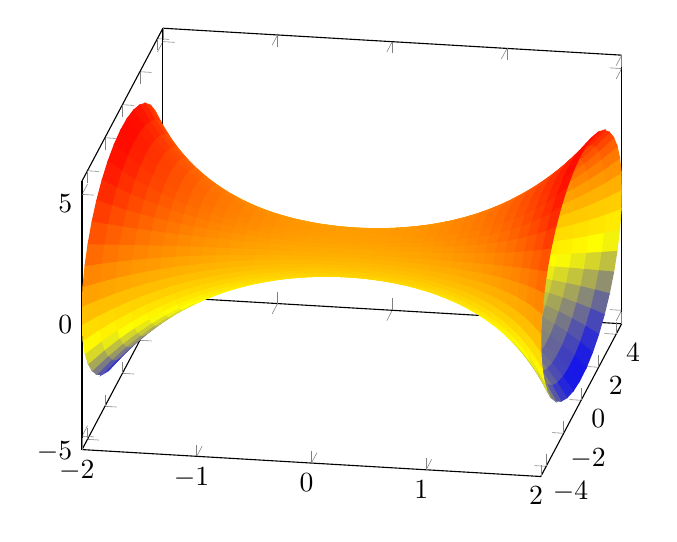
\begin{tikzpicture}
 \begin{axis}[view={10}{30}]
  \addplot3[surf,shader=flat,
  samples=40,
  domain=-2:2,y domain=0:2*pi,
  z buffer=sort]
  ({x},{0.833*cosh(x/0.833) * cos(deg(y))}, {0.833*cosh(x/0.833) * sin(deg(y))});
 \end{axis}
\end{tikzpicture}
\end{center}
\end{ans}
\begin{qns}[Euler-Lagrange for higher order derivatives]
Show from first principles that the functional $I[x]=\int_{t_1}^{t_2}f(t,x,\dot{x},\ddot{x})dt$ is extremized, for variations with both $x(t)$ and $\dot{x}(t)$ fixed at $t_1$ and $t_2$, by solutions of the equation
$$\frac{\partial f}{\partial x}-\frac{d}{dt}\frac{\partial f}{\partial\dot{x}}+\frac{d^2}{dt^2}\frac{\partial f}{\partial\ddot{x}}=0$$
Hence find the function $x(t)$ with $x(1) = 1$, $\dot{x}(1))=-2$,  $x(2)=0.25$ and $\dot{x}(2)=-0.25$ that minimises $\int_1^2t^4\ddot{x}(t)^2dt$.
\end{qns}
\begin{ans}
We have $\delta I=I[x+\delta x]-I[x]$,
\begin{eqnarray}
\delta I&=&\int_{t_1}^{t_2}f(t,x+\delta x,\dot{x}+\delta\dot{x},\ddot{x}+\delta\ddot{x})dt-\int_{t_1}^{t_2}f(t,x,\dot{x},\ddot{x})dt\nonumber\\&=&-\int_{t_1}^{t_2}f(t,x,\dot{x},\ddot{x})dt+\int_{t_1}^{t_2}f(t,x,\dot{x},\ddot{x})+\delta x\frac{\partial f}{\partial x}+\delta\dot{x}\frac{\partial f}{\partial\dot{x}}+\delta\ddot{x}\frac{\partial f}{\partial\ddot{x}}+\dots dt\nonumber\\&=&\int_{t_1}^{t_2}\delta x\frac{\partial f}{\partial x}dt+\bigg[\delta x\frac{\partial f}{\partial\dot{x}}\bigg]_{t_1}^{t_2}-\int_{t_1}^{t_2}\delta x\frac{d}{dt}\frac{\partial f}{\partial\dot{x}}dt+\bigg[\delta\dot{x}\frac{\partial f}{\partial\ddot{x}}\bigg]_{t_1}^{t_2}-\int_{t_1}^{t_2}\delta\dot{x}\frac{d}{dt}\frac{\partial f}{\partial\ddot{x}}dt\nonumber\\&=&\int_{t_1}^{t_2}\delta x\bigg[\frac{\partial f}{\partial x}-\frac{d}{dt}\frac{\partial f}{\partial\dot{x}}+\frac{d^2}{dt^2}\frac{\partial f}{\partial\ddot{x}}\bigg]dt+\bigg[\delta x\frac{\partial f}{\partial\dot{x}}+\delta\dot{x}\frac{\partial f}{\partial\ddot{x}}-\delta x\frac{d}{dt}\frac{\partial f}{\partial\ddot{x}}\bigg]_{t_1}^{t_2}\nonumber
\end{eqnarray}
We require the second term to be zero since $x(t)$ and $\dot{x}(t)$ are fixed at $t_1$ and $t_2$. We thus have
$$\frac{\delta I}{\delta x}=\int_{t_1}^{t_2}\frac{\partial f}{\partial x}-\frac{d}{dt}\frac{\partial f}{\partial\dot{x}}+\frac{d^2}{dt^2}\frac{\partial f}{\partial\ddot{x}}dt=0\implies \frac{\partial f}{\partial x}-\frac{d}{dt}\frac{\partial f}{\partial\dot{x}}+\frac{d^2}{dt^2}\frac{\partial f}{\partial\ddot{x}}=0$$
Now consider $I[\ddot{x},t]=\int_1^2t^4\ddot{x}(t)^2dt$. Upon extremizing, we have $\frac{\partial f}{\partial x}=0$, $\frac{d}{dt}\frac{\partial f}{\partial\dot{x}}=\frac{d}{dt}0=0$, and so $\frac{d^2}{dt^2}\frac{\partial f}{\partial\ddot{x}}=0\implies \ddot{x}=\frac{A}{2}t^{-4}+\frac{B}{2}t^{-3}$. We thus have
$$\dot{x}=-\frac{A}{6}t^{-3}-\frac{B}{4}t^{-2}+C,~x=\frac{A}{(-3)2(-2)}t^{-2}-\frac{B}{2(-2)}t^{-1}+Ct+D$$
Imposing boundary conditions $$x(1)=1\implies \frac{A}{12}+\frac{B}{4}+C+D=1,\quad \dot{x}(1)=-2\implies-\frac{A}{6}-\frac{B}{4}+C=-2$$ $$x(2)=0.25\implies\frac{A}{(-3)2(-2)}2^{-2}-\frac{B}{2(-2)}2^{-1}+2C+D,\quad\dot{x}(2)=-0.25\implies-\frac{A}{6}2^{-3}-\frac{B}{4}2^{-2}+C$$
We thus have $B=6$, $A=C=D=0$, and so $x=t^{-2}$.
\end{ans}
\newpage
\begin{qns}[Fermat]
State Fermat's principle governing the paths traced by light rays in a medium. A horizontally stratified medium has refractive index $\mu(z)=\sqrt{a-bz}$ where $z$ is height and $a$ and $b$ are positive constants. Prove that the path of a light ray within a vertical plane in this medium is an inverted parabola. Show further that all such parabolas have their directrix in the plane $z = a/b$. [The directrix of a parabola in the standard form $y^2=4\alpha x$ is the line $x=-\alpha$.]
\end{qns}
\begin{ans}
Fermat's principle of geometric optics states that the path taken by a light ray from point A to point B in a material of variable refractive index $\mu(\mathbf{r})$ minimizes the optical path length, $P=\int_A^B\mu(\mathbf{r})dl$, where $dl=\sqrt{dx^2+dy^2+dz^2}$ is the length element. Equivalently, the time taken for the light to travel through the path is minimized.\\[5pt]
Consider the $x$-$z$ plane, $P=\int\sqrt{a-bz}\sqrt{dx^2+dz^2}$. Firstly, suppose $z$ is a function of $x$,
$$P[z]=\int\sqrt{a-bz}\sqrt{1+z'^2}dx$$
Since there is no $x$ dependence in the integrand, $\frac{\delta P}{\delta x}=0$ and so the first integral gives $z'\frac{\partial f}{\partial z'}-f$ being a constant, i.e.
$$z'^2\bigg(\frac{z'\sqrt{a-bz}}{\sqrt{1+z'^2}}\bigg)-\sqrt{a-bz}\sqrt{1+z'^2}=\sqrt{k}\implies z'=\sqrt{\frac{a-bz-k}{k}}$$
where $k$ is some constant. This simplifies to $$z=-\frac{b}{4k}(x-c)^2+\frac{a-k}{b}\implies (x-c)^2=\bigg(z-\frac{a-k}{b}\bigg)\bigg(-\frac{4k}{b}\bigg)$$ 
Comparing to the equation of a parabola, $p^2=4\alpha q$, which has directrix at $q=-\alpha$ then $p=x-c$ and $q=z-\frac{a-k}{b}$, and $\alpha=-\frac{k}{b}$. So $z-\frac{a-k}{b}=\frac{k}{b}\implies z=\frac{a}{b}$. This is the desired equation of the directrix. 
\end{ans}
\begin{qns}[Fermat]
Given that the refractive index $\mu(\mathbf{r})$ of some material equals $|\boldsymbol{\nabla}f|$ for some function $f(\mathbf{r})$, show that the optical path length $\int_A^B\mu dl$ between points A and B in the material is no less than $f(B)-f(A)$ with equality if and only if the path is orthogonal to the family of surfaces of constant $f$. Deduce that such `orthogonal' trajectories satisfy Fermat's principle.
\end{qns}
\begin{ans}
The optical path length is $P=\int_A^B|\boldsymbol{\nabla}f|dr$, but
$$|\boldsymbol{\nabla}f|dl\geq|\boldsymbol{\nabla}f|dl\cos\theta=\boldsymbol{\nabla}f\cdot d\mathbf{l}=df\implies P\geq\int_A^Bdf=f(B)-f(A)$$
The equality holds when $\cos\theta=1\implies\theta=0$, i.e. $\boldsymbol{\nabla}f$ is parallel to $d\mathbf{l}$, i.e. the path  $d\mathbf{l}$ is orthogonal to family of surfaces of constant $f$.
Hence, the path must be orthogonal to the surface of constant f. When such orthogonal trajectories are taken, $\frac{\delta P}{\delta y}=\frac{\partial g}{\partial y}-\frac{d}{dx}\frac{\partial g}{\partial y'}=0$ and $\frac{\delta P}{\delta z}=\frac{\partial g}{\partial z}-\frac{d}{dx}\frac{\partial g}{\partial z'}=0$. Hence, the optical path length is a minimum, which satisfies the Fermat's principle.
\end{ans}
\begin{qns}[Lagrangian]
A particle of unit mass moves in a plane, with polar coordinates $(r,\theta)$, under the influence of a central force derived from a potential $V (r)$. Write down the action functional for this problem and use Hamilton's principle to find differential equations for $r(t)$ and $\theta(t)$. What is the physical interpretations of these equations? Given that a particle's trajectory is $r=a\sin\theta$ for some constant $a$, deduce that there exists a constant $E$ such that $(V-E)$ is directly proportional to $r^{-4}$.
\end{qns}
\begin{ans}
Let $\mathbf{x}=(r\cos\theta,r\sin\theta)^T$ be the position vector of the unit mass. We have $|\mathbf{\dot{x}}|=\sqrt{\dot{r}^2+r^2\dot{\theta}^2}$. Let the Lagrangian be $\mathcal{L}=T-V$, we have $S[r,\theta]$ to be the action-functional
$$S[r,\theta]=\int_{t_0}^{t_1}\mathcal{L}(r,\dot{r},\theta,\dot{\theta};t)dt$$
where $\mathcal{L}=\frac{1}{2}\dot{r}^2+\frac{1}{2}r^2\dot{\theta}^2-V(r)$. Using the Euler-Lagrange equations, we have
\begin{itemize}
    \item $\frac{d}{dt}r^2\dot{\theta}=0$, which gives us the conservation of angular momentum;
    \item $\ddot{r}-\frac{k^2}{r^3}+\frac{dV}{dr}=0$, where $k^2/r^3=r\dot{\theta}^2$ is the centrifugal force, such that $\ddot{r}=-\frac{d}{dr}V_{eff}$ where $V_{eff}=V-\frac{k^2}{2r^2}$, which gives Newton's Second Law.
\end{itemize}
Since $\mathcal{L}$ has no explicit dependence on $t$, so
$$d\mathcal{L}=\frac{\partial\mathcal{L}}{\partial t}dt+\frac{\partial\mathcal{L}}{\partial r}dr+\frac{\partial\mathcal{L}}{\partial \dot{r}}d\dot{r}+\frac{\partial\mathcal{L}}{\partial\theta}d\theta+\frac{\partial\mathcal{L}}{\partial\dot{\theta}}d\dot{\theta}\implies\frac{d\mathcal{L}}{dt}=\frac{\partial\mathcal{L}}{\partial t}+\frac{d}{dt}\bigg(\dot{r}\frac{\partial\mathcal{L}}{\partial\dot{r}}+\dot{\theta}\frac{\partial\mathcal{L}}{\partial\theta}\bigg)$$
Since $\frac{\partial\mathcal{L}}{\partial t}=0$, we then have the first integral to be
$$\frac{d}{dt}\bigg(\dot{r}\frac{\partial\mathcal{L}}{\partial\dot{r}}+\dot{\theta}\frac{\partial\mathcal{L}}{\partial\theta}-\mathcal{L}\bigg)=0\implies E= \dot{r}\frac{\partial\mathcal{L}}{\partial\dot{r}}+\dot{\theta}\frac{\partial\mathcal{L}}{\partial\theta}-\mathcal{L}=\dot{r}\dot{r}+\dot{\theta}r^2\dot{\theta}-\frac{1}{2}\dot{r}^2-\frac{1}{2}r^2\dot{\theta}^2+V(r)$$
where $E$ is a constant. This is the statement of the conservation of energy.\\[5pt]
Given $r=a\sin\theta$, we have
$$E=\frac{1}{2}\dot{r}^2+\frac{1}{2}\dot{\theta}^2r^2+V(r)=\frac{1}{2}a^2\cos^2\theta\dot{\theta}^2+\frac{1}{2}a^2\dot{\theta}^2\sin^2\theta+V(r)=\frac{1}{2}a^2\dot{\theta}^2+V(r)\implies E-V=\frac{1}{2}a^2\frac{k^2}{r^4}$$
Hence, $V-E$ is directly proportional to $r^{-4}$.
\end{ans}
\begin{qns}[Lagrange Multiplier]
The temperature of a point on the unit sphere $x^2+y^2+z^2=1$ is given by $T(x,y,z)=1+xyz$. Find the points of maximum and minimum temperature on the sphere. What are their temperatures?
\end{qns}
\begin{ans}
Using Lagrange multiplier, we have $$\phi(x,y,z;\lambda)=(1+xyz)-\lambda(x^2+y^2+z^2-1)$$
To find the minimum and maximum $T$, $\frac{\partial\phi}{\partial\lambda}=0$ recovers the constraint equation, $\frac{\partial\phi}{\partial x}=0\implies xyz-2\lambda x^2=0$, $\frac{\partial\phi}{\partial y}=0\implies xyz-2\lambda y^2=0$ and lastly, $\frac{\partial\phi}{\partial z}=0\implies xyz-2\lambda z^2=0$. Adding the last three together, we have $3xyz=2\lambda(x^2+y^2+z^2)=2\lambda$. Hence, $x=\pm1/\sqrt{3}$. By symmetry, we have $y=z=\pm1/\sqrt{3}$. Lastly, we check the values for minimum and maximum $T$, which are $\{(-u,-u,-u),(-u,u,u),(u,-u,u),(u,u,-u)\}$ and $\{(u,u,u),(-u,-u,u),(-u,u,-u),(u,-u,-u)\}$ respectively, where $u=\frac{1}{\sqrt{3}}$. 
\end{ans}
\begin{qns}[Lagrange Multiplier]
A coal box, in the shape of a cuboid, is to be placed flush against a wall so that only its top, front and two ends are visible. How should the height $h$ and the depth $d$ be chosen so as to minimize the visible surface area $A$ under the constraint that the box has a given volume $V$?
\end{qns}
\begin{ans}
Using Lagrange multiplier, we have
$$\phi(h,d,l;\lambda)=hl+dl+2dh-\lambda(ldh-V)$$
We want to minimize $A$. $\frac{\partial\phi}{\partial\lambda}=0$ recovers the constraint on $V$; $\frac{\partial\phi}{\partial d}=0\implies l+2h-\lambda lh=0$; $\frac{\partial\phi}{\partial h}=0\implies l+2d-\lambda ld=0$; $\frac{\partial\phi}{\partial l}=0\implies h+d-\lambda dh=0$. With $l=\frac{V}{dh}$ and $\lambda=\frac{h+d}{dh}$, we obtain two equations $\frac{V}{h}+2hd-\frac{V(h+d)}{dh}=0$ and $\frac{V}{d}+2hd-\frac{V(h+d)}{dh}=0$. Taking their differences, we obtain $h=d$. Finally, we obtain $h=(0.5V)^{1/3}$.
\end{ans}
\newpage
\begin{qns}[Constrained variation]
Extremize the functional
$$F[y]=\int_0^a(y'^2+yy'+2y)dx$$
with the boundary conditions $y(0)=y(a)=0$ and subject to the constraint $\int_0^aydx=\ell$, where $\ell$ is a constant.
\end{qns}
\begin{ans}
We construct
$$\phi[y]=F[y]-\lambda\bigg(\int_0^aydx-\ell\bigg)\implies\phi[y]=\int_0^ay'^2+yy'+(2-\lambda)ydx+\lambda\ell$$
Since the integrand (let it be $g$) is not explicitly dependent on $x$, then by the chain rule, we have $0=\frac{\partial g}{\partial x}=\frac{d}{dx}g-\frac{\partial g}{\partial y}y'-\frac{\partial g}{\partial y'}y''=\frac{d}{dx}(g-y'\frac{\partial g}{\partial y'})$ and so the first integral gives
$$y'^2+yy'+(2-\lambda)y-2y'^2-yy'=c\implies -y'^2+(2-\lambda)y=-c$$
where $c$ is a constant. Imposing boundary conditions $y(0)=0\implies c=4(2-\lambda)^2x_0^2$ and $y(a)=0\implies x_0=\frac{a}{2}$. Finally, the Lagrange multiplier is obtained by using the constraint $\int_0^aydx=\ell$, and hence
$$y=6\ell a^{-3}x(a-x)$$
\end{ans}
\begin{qns}[Isoperimetric problem]
An area A of a field is enclosed by a length $l$ of flexible fencing with its ends attached a distance $a$ apart on a straight wall, where $a<l<0.5\pi a$. What shape maximizes $A$?
\end{qns}
\begin{ans}
We have $A=\int_0^aydx$, $l=\int_0^a\sqrt{1+y'^2}dx$. Consider the functional
$$\phi_\lambda[y]=\int_0^aydx-\lambda\int_0^a\sqrt{1+y'^2}dx+\lambda l$$
Maximizing $A$ under constraint is the same as maximizing $\phi_\lambda$ without constraint. Since the integrand has no explicit $x$ dependence, using first integral,
$$y'\frac{\partial}{\partial y'}(y-\lambda\sqrt{1+y'^2})-(y-\lambda\sqrt{1+y'^2})=-y'\frac{\lambda y'}{\sqrt{1+y'^2}}-(y-\lambda\sqrt{1+y'^2})=\frac{\lambda}{\sqrt{1+y'^2}}-y$$
which is a constant, $c$. Rearranging, 
$$\int\frac{y+c}{\sqrt{\lambda^2-(y+c)^2}}dy=\int dx\implies\lambda^2-(y+c)^2=(x+k)^2$$
which describes a circle centred at $(-k,-c)$ with radius $\lambda$. $k$ translates the fence along the straight wall/axis. We can set $k=0$. When $x=\pm0.5a$, $y=0$, we have $\lambda=\sqrt{c^2+0.25a^2}$, so $l=2\sqrt{c^2+0.25a^2}\tan^{-1}(a/2c)$.
$$(y+c)^2+x^2=c^2+\frac{a^2}{4}$$
where $0.5a<\sqrt{c^2+0.25a^2}\tan^{-1}(a/2c)<0.25\pi a$.
\end{ans}
\newpage
\begin{qns}[Rayleigh Ritz]
A Sturm-Liouville eigenvalue problem for functions $y(x)$ satisfying $y(\pm1)=0$ has the equation
$$-(1+x^2)y''-2xy'-\lambda y$$
Use the Rayleigh-Ritz method with trial function $y_1=1-x^2$ to obtain an upper bound on the lowest eigenvalue $\lambda$. Show that a better bound is obtained from the trial function $y_2=\cos(\pi x/2)$. Explain how a further improvement could be achieved by considering $y_1$ and $y_2$ in combination. [$\int_{-1}^1x^2\sin^2(\pi x/2)dx=\frac{1}{3}+\frac{2}{\pi^2}$]
\end{qns}
\begin{ans}
The Sturm-Liouville operator is $-\frac{d}{dx}(1+x^2)\frac{d}{dx}$, so we have $F[y]=\int_{-1}^1(1+x^2)y'^2dx$ and $G[y]=\int_{-1}^1y^2dx$. Given the trial function $y_1=1-x^2$,
$$F[y_1]=\int_{-1}^1(1+x^2)(-2x)^2dx=\frac{64}{15}$$
$$G[y_1]=\int_{-1}^1(1-x^2)^2dx=\frac{16}{15}$$
Hence, $\lambda\leq\Lambda[y_1]=\frac{F[y_1]}{G[y_1]}=4$, which is the upper bound. Try again with $y_2=\cos(0.5\pi x)$,
$$F[y_2]=\int_{-1}^1(1+x^2)\frac{\pi^2}{4}\sin^2(0.5\pi x)dx=\frac{\pi^2}{8}[x-\pi^{-1}\sin(\pi x)]_{-1}^1+\frac{\pi^2}{12}+\frac{1}{2}=\frac{\pi^2}{3}+\frac{1}{2}$$
$$G[y_2]=\int_{-1}^1\cos^2(0.5\pi x)dx=1$$
Hence $\Lambda[y_2]=\frac{F[y_2]}{G[y_2]}=\frac{\pi^2}{3}+\frac{1}{2}<\Lambda[y_1]$, and hence we obtain a better bound with $y_2$. To further obtain a better improvement, we can have a trial solution $y_3=a_1y_1+a_2y_2$, where $a_1$ and $a_2$ are parameters. This method is still valid even if one of $y_1$, $y_2$ is a worse trial function. We can find $a_1$ and $a_2$ by minimizing $\Lambda[y_3]$ with respect to their ratio $a_1/a_2$.
\end{ans}
\begin{qns}[Rayleigh Ritz]
The differential equation governing small transverse displacements $y(x)$ of a string with fixed endpoints at $x = 0$ and $x=\pi$ is $$y''+\omega^2f(x)y=0$$ where $\omega$ is the angular frequency of the vibration and $f$ is a positive function. Show that the allowed values of $\omega^2$ are given by the stationary values of the ratio of functionals $\Omega^2=F/G$, where $F=\int_0^\pi y'^2dx$ and $G=\int_0^\pi fy^2dx$. Use this fact to find an approximate value for the angular frequency of the fundamental mode when $f=1+\epsilon\sin(x)$, assuming $\epsilon<<1$.
\end{qns}
\begin{ans}
In SL form $\mathcal{L}y=\lambda w(x)y$, we have $\mathcal{L}=-\frac{d^2}{dx^2}$, $\lambda=\omega^2$ and $f(x)=w(x)$. Let $F[y]=\int_0^\pi y'^2dx$ and $G[y]=\int_0^\pi fy^2dx$, so
$$\delta F=F[y+\delta y]-F[y]=\int_0^\pi(y'+\delta y')^2dx-\int_0^\pi y'^2d=-\int_0^\pi 2y''\delta ydx+[y'\delta y]_0^\pi=\int_0^\pi2\mathcal{L}y\delta ydx$$
where $y$ is fixed at $x=0$ and $x=\pi$.
$$\delta G=G[y+\delta y]-G[y]=\int_0^\pi f(y+\delta y)^2-\int_0^\pi fy^2dx=\int_0^\pi 2\delta yfydx$$
So we have $\Omega^2=\frac{F}{G}$ and then
$$\delta(\Omega^2)=\frac{F+\delta F}{G+\delta G}-\frac{F}{G}=\frac{1}{G}(F+\delta F)\bigg(1-\frac{\delta G}{G}+...\bigg)-\frac{F}{G}=\frac{1}{G}(\delta F-\Omega^2\delta G)$$
Extremizing gives $\frac{\delta F}{\delta y}=\Omega^2\frac{\delta G}{\delta y}\implies\mathcal{L}y=\Omega^2fy$. So $\Omega^2$ is extremized by the extremal values $\lambda=\omega^2$ from the SL equation.\\[5pt]
The fundamental mode is $y=\sin(x)$ and so
$$F[y]=\int_0^\pi(-\sin x)^2=\frac{\pi}{2}$$
$$G[y]=\int_0^\pi(1+\epsilon\sin x)\sin^2xdx=\frac{\pi}{2}+\epsilon[-\cos x+3^{-1}\cos^3x]_0^\pi=\frac{\pi}{2}+\frac{4\epsilon}{3}$$
Hence
$$\Omega^2[y]=\frac{F[y]}{G[y]}=\bigg(1+\frac{4\epsilon}{3}\frac{2}{\pi}\bigg)^{-1}\approx 1-\frac{8\epsilon}{3\pi}$$
where $\epsilon<<1$.
\end{ans}
\begin{qns}[Rayleigh Ritz]
Show that $\psi_0=e^{-0.5x^2}$ is an eigenfunction of the operator
$$\mathcal{L}=-\frac{d^2}{dx^2}+(x^2-1)$$
acting on functions $\psi(x)$ for which $\psi\rightarrow0$ as $|x|\rightarrow\infty$, and find the corresponding eigenvalue $\lambda_0$. This is in fact the lowest eigenvalue.\\[5pt]
Use the Rayleigh Ritz method with trial function
$$\tilde{\psi}_0=b(a^2-x^2)$$
for $|x|<a$ and 0 for $|x|\geq a$, where $a$ and $b$ are adjustable parameters, to obtain an approximation $\overline{\lambda}_0$ to $\lambda_0$. Comment on the sign of $\overline{\lambda}_0-\lambda_0$.
\end{qns}
\begin{ans}Since $\psi_0=e^{-0.5x^2}$, then
$$\mathcal{L}\psi_0=-(x^2-1)e^{-0.5x^2}+(x^2-1)e^{-0.5x^2}=0\psi_0$$
where the eigenvalue $\lambda_0=0$.\\[5pt]
The Sturm-Liouville problem has $p(x)=1$, $q(x)=x^2-1$ and $w(x)=1$. Try trial function $\tilde{\psi}_0=b(a^2-x^2)$ for $|x|<a$, then
$$F[\tilde{\psi}_0]=\langle\tilde{\psi}_0|\mathcal{L}\tilde{\psi}_0\rangle=b^2\int_{-a}^a(a^2-x^2)(2+(x^2-1)(a^2-x^2))dx=2b^2\bigg(\frac{8}{105}a^7-\frac{8}{15}a^5+\frac{4}{3}a^3\bigg)$$
$$G[\tilde{\psi}_0]=\int_{-a}^ab^2(a^2-x^2)^2dx=2b^2\bigg(a^5-\frac{2}{3}a^5+\frac{1}{5}a^4\bigg)=2b^2\frac{8}{15}a^5$$
Hence 
$$\Lambda[\tilde{\psi}_0]=\frac{F[\tilde{\psi}_0]}{G[\tilde{\psi}_0}=\frac{15}{8}\bigg(\frac{8}{105}a^2-\frac{8}{15}+\frac{4}{3}a^{-2}\bigg)$$
We extremize $\Lambda$ with respect to $a^2$, then
$$0=\frac{d\Lambda}{da^2}=\frac{15}{8}\bigg(\frac{8}{105}-\frac{4}{3a^4}\bigg)\implies a^4=\frac{35}{2}\implies\Lambda=\sqrt{\frac{10}{7}}-1>0$$
$\Lambda[\psi]=\overline{\lambda}_0\geq\lambda_0$ is always true if $F[\psi]>0$ $\forall\psi$, i.e. Rayleigh-Ritz always yield an overestimate of the lowest eigenvalue. Equality follows if $\psi=\psi_0$.
\end{ans}
\newpage
\section{Lent Example Sheet 2}
\subsection*{Laplace's and Poisson's equation}
\begin{qns}[Cartesian]
The function $\Phi(x,y)$, defined in the semi-infinite strip $0\leq x\leq1$, $y\geq0$, satisfies $\nabla^2\Phi=0$ (two-dimensional Laplace equation) subject to the boundary conditions $\Phi(0,y)=\Phi(1,y)=0$, $\Phi(x,0)=x(1-x)$, $\Phi(x,\infty)=0$. Use the method of separation of variables in Cartesian coordinates to find $\Phi(x,y)$. Hence find $\int_0^1\frac{\partial\Phi}{\partial y}|_{y=0}dx$, leaving your answer as an infinite series.
\end{qns}
\begin{ans}
Use the method of separation of variables $\Phi(x,y)=X(x)Y(y)$ such that $$\frac{X''}{X}=-\frac{Y''}{Y}=-\lambda$$ where $\lambda>0$ is constant. Motivated by the boundary conditions, $\Phi(0,y)=\Phi(1,y)=0$, we have $X(x)=c_1\sin(\sqrt{\lambda}x)+c_2\cos(\sqrt{\lambda}x)$ such that $\sqrt{\lambda}=n\pi$ and $c_2=0$ due to the boundary conditions, where $n\in\mathbb{Z}^+$. Also, $Y(y)=c_3e^{n\pi y}+c_4e^{-n\pi y}$. So the general solution is
$$\Phi(x,y)=\sum_{n=1}^\infty(c_1\sin(n\pi x))(c_3e^{n\pi y}+c_4e^{-n\pi y})$$
Imposing $\Phi(x,\infty)=0\implies c_3=0$ and $x(1-x)=\Phi(x,0)=\sum_{n=1}^\infty A_n\sin(n\pi x)$. Using Fourier series,
$$A_n=\frac{2}{1}\int_0^1x(1-x)\sin(n\pi x)dx=2\int_0^1x\sin(n\pi x)dx-2\int_0^1x^2\sin(n\pi x)dx=-\frac{4}{n^3\pi^3}[\cos(n\pi x)]_0^1$$
which is $\frac{8}{n^3\pi^3}$ for odd $n$ and zero for even $n$. Hence, after re-indexing,
$$\Phi(x,y)=\frac{8}{\pi^3}\sum_{n=0}^\infty\frac{1}{(2n+1)^3}\sin((2n+1)\pi x)e^{-(2n+1)\pi y}$$
Finally,
$$\int_0^1\frac{\partial\Phi}{\partial y}\bigg|_{y=0}dx=\int_0^1\sum_{n=0}^\infty-\frac{8}{\pi^2(2n+1)^2}\sin((2n+1)\pi x)dx=-\frac{8}{\pi^3}\sum_{n=0}^\infty\frac{2}{(n+1)^3}=-\frac{16}{\pi^3}\sum_{n=0}^\infty\frac{1}{(n+1)^3}$$
\end{ans}
\newpage
\begin{qns}[Plane Polar]
A solute with diffusivity $\kappa$, of concentration $\Phi(r,\theta)$ in plane polar coordinates, both surrounds and fills a cylinder of radius $a$. The boundary of the cylinder is permeable and the solute diffuses through it in such a way that the flux has normal component $F\cos2\theta$ at $r = a$, where $F$ is a constant. Assuming a steady state, find the distribution of solute in the interior of the cylinder. Why does your answer include an arbitrary constant? How is it possible for there to be a constant flux of solute through the boundary of the cylinder and yet for the concentration within to remain fixed?
\end{qns}
\begin{ans}
At steady state, we solve $\nabla^2\Phi=0$, subjected to the following constraints:
\begin{itemize}
    \item The boundary condition is the normal component of flux at $r=a$: 
$$-\kappa\boldsymbol{\nabla}\Phi(r,\phi)\cdot\boldsymbol{\hat{r}}|_{r=a}=F\cos(2\phi)$$
\item $\Phi(r,\phi)$ is periodic:
$$\Phi(r,\phi)=\Phi(r,\phi+2\pi)$$
\item $\Phi$ is finite at $r=0$.
\end{itemize}
Using separation of variables, $\Phi(r,\phi)=R(r)\Psi(\phi)$, then
$$0=\frac{\Psi}{r}\frac{d}{dr}\bigg(r\frac{dR}{dr}\bigg)+\frac{R}{r^2}\frac{d^2\Psi}{d\phi^2}\implies \psi''+\lambda\psi=0,~\frac{r}{R}\frac{d}{dr}\bigg(r\frac{dR}{dr}\bigg)=\lambda$$
where $\lambda$ is a constant. For the angular equation, try $\Psi(\phi)=e^{k\phi}$, then $k=\pm i\sqrt{\lambda}$, then $\Psi(\phi)=A+B\phi$ for $\lambda=0$ and $\Psi(\phi)=A\sin\sqrt{\lambda}\phi+B\cos\sqrt{\lambda}\phi$ for $\lambda\neq 0$. Periodicity implies $\lambda=n^2$, where $n\in\mathbb{Z}$, and $B=0$ when $n=0$. For the radial equation, try $R=r^\gamma$ when $n\neq 0$, then $R(r)=Cr^n+Dr^{-n}$. When $n=0$, $R(r)=C+D\ln(r)$. For both cases, $C=0$ since $R(r=0)$ is finite. Combining all these facts give:
$$\Phi(r,\phi)=A_0+\sum_{n=1}^\infty r^n(A_n\cos(n\phi)+B_n\sin(n\phi))$$
The flux is $\mathbf{F}=-\kappa\boldsymbol{\nabla}\Phi$, and imposing the boundary condition gives
$$F\cos(2\phi)=-\kappa\sum_{n=1}^\infty na^{n-1}(A_n\cos(n\phi)+B_n\sin(n\phi))$$
Then, $A_n=0$ $\forall n\neq 2$ and $B_n=0$ $\forall n$. We thus have $A_2=\frac{F}{-2a\kappa}$. Hence, the solution is $$\Phi(r,\phi)=A_0-\frac{Fr^2}{2a\kappa}\cos(2\phi)$$ 
$A_0$ is a constant, which determines the concentration of solute at $r=0$. The concentration within the cylinder is constant, since the amount of solute flowing in is equal to that flowing out. The transition between radially in and out, occurs when $\phi=\frac{\pi}{4}$.
\end{ans}
\newpage
\begin{qns}[Plane Polar]
A single-valued potential $\Phi(r,\theta)$, in plane polar coordinates, satisfies $\nabla^2\Phi=0$ inside a cylindrical annulus $a < r < b$. On $r = b$, $\Phi=0$ $\forall\theta$. On $r = a$, $\Phi=0$ for $-\pi<\theta\leq0$ and $\Phi=1$ for $0<\theta\leq\pi$. Find $\Phi(r,\theta)$ inside the annulus.
\end{qns}
\begin{ans}
$\Phi(r,\theta)$ satisfies $\nabla^2\Phi=0$ for $a<r<b$ and satisfies the following:
\begin{itemize}
    \item $\Phi(b,\theta)=0$ $\forall\theta$;
    \item $\Phi(a,\theta)=0$ $\forall\theta\in(-\pi,0]$;
    \item $\Phi(a,\theta)=1$ $\forall\theta\in(0,\pi]$;
    \item Single-valued:  $\Phi(r,\theta)=\Phi(r,\theta+2\pi)$
\end{itemize}
Using separation of variables, $\Phi(r,\theta)=R(r)\Psi(\theta)$, then
$$0=\frac{\Psi}{r}\frac{d}{dr}\bigg(r\frac{dR}{dr}\bigg)+\frac{R}{r^2}\frac{d^2\Psi}{d\theta^2}\implies \Psi''+\lambda\Psi=0,\quad\frac{r}{R}\frac{d}{dr}\bigg(r\frac{dR}{dr}\bigg)=\lambda$$
where $\lambda$ is a constant. For the angular equation, try $\Psi(\theta)=e^{k\theta}$, then $k=\pm i\sqrt{\lambda}$, then $\Psi(\theta)=A+B\theta$ for $\lambda=0$ and $\Psi(\theta)=A\sin(\sqrt{\lambda}\theta)+B\cos(\sqrt{\lambda}\theta)$ for $\lambda\neq 0$. Periodicity implies $\lambda=n^2$, where $n\in\mathbb{Z}$, and $B=0$ when $n=0$. For the radial equation, try $R=r^n$ when $n\neq 0$, then $R(r)=Cr^n+Dr^{-n}$. When $n=0$, $R(r)=C+D\ln(r)$. Combining all these facts give:
$$\Phi(r,\theta)=A_0+B_0\ln(r)+\sum_{n=1}^\infty(A_nr^n+B_nr^{-n})\sin(n\theta)+\sum_{n=1}^\infty(C_nr^n+D_nr^{-n})\cos(n\theta)$$
Impose boundary conditions
$$\Phi(b,\theta)=0\implies A_0=-B_0\ln(b),\quad B_n=-A_nb^{2n},\quad D_n=-C_nb^{2n}$$
$$1=\Phi(a,0<\theta<\pi)=B_0\ln\frac{a}{b}+\sum_{n=1}^\infty A_n(a^n-b^{2n}a^{-n})\sin(n\theta)+\sum_{n=1}^\infty C_n(a^n-b^{2n}a^{-n})\cos(n\theta)$$
Using Fourier series,
$$B_0=\frac{1}{2\pi}\frac{1}{\ln(a/b)}\int_0^\pi d\theta=\frac{1}{2\ln(a/b)}$$
$$B_n(a^n-b^{2n}a^{-n})=\frac{1}{\pi}\int_0^\pi\cos(n\theta)d\theta=0$$
$$A_n(a^n-b^{2n}a^{-n})=\frac{1}{\pi}\int_0^\pi\sin(n\theta)d\theta=\frac{2}{\pi n}$$
for odd $n$ and zero otherwise. Thus, the solution inside the annulus is
$$\Phi(r,\theta)=\frac{\ln(r/b)}{2\ln(a/b)}+\frac{2}{\pi}\sum_{p=1}^\infty\frac{\sin((2p+1)\theta)}{(2p+1)(a^{2p+1}-b^{2(2p+1)}a^{-(2p+1)})}(r^{2p+1}-b^{2(2p+1)}r^{-(2p+1)})$$
\end{ans}
\newpage
\begin{qns}[Plane polar]
The axis of a solid cylinder of radius $a$ coincides with the $z$-axis of cylindrical polar coordinates $(r,\theta,z)$. Heat flows past the cylinder such that the temperature $T$ inside and outside, i.e. for $r < a$ and $r > a$, is independent of $z$ and satisfies $\nabla^2T=0$. Find $T$ subject to the following boundary conditions: $T$ finite at $r = 0$ and $T\sim Gr\cos\theta$ as $r\rightarrow\infty$, where $G$ is a constant; $T$ continuous at $r = a$ but $\frac{\partial T}{\partial r}(a^+,\theta)=\beta\frac{\partial T}{\partial r}(a^-,\theta)$ for constant $\beta$ ($0<\beta<1$). What is the physical meaning of the constants $G$ and $\beta$? [$a^+$ denotes the limit $r\rightarrow a$ from $r > a$ and $a^-$ denotes the limit $r\rightarrow a$ from $r<a$.]
\end{qns}
\begin{ans}
$T(r,\theta)$ satisfy $\nabla^2T=0$, for the regions $r>a$ and $r<a$. $T$ further satisfy
\begin{itemize}
    \item $T$ is finite at $r=0$;
    \item $\boldsymbol{\nabla}T(r=a)$ is discontinuous, i.e.
    $$\frac{\partial T}{\partial r}(r=a^+,\theta)=\beta\frac{\partial T}{\partial r}(r=a^-,\theta)$$
    for some constant $\beta$, $0<\beta<1$;
    \item $T$ has an asymptotic form $Gr\cos\theta$ as $r\rightarrow\infty$;
    \item $T$ is single-valued, i.e. $T(r,\theta)=T(r,\theta+2\pi)$;
    \item $T(r=a)$ is continuous.
\end{itemize}
After ensuring the single-valuedness, finiteness and asymptotics of $T$, we obtain
$$T(r<a,\theta)=A_0+\sum_{n=1}^\infty r^n(A_n\sin(n\theta)+C_n\cos(n\theta))$$
$$T(r>a,\theta)=Gr\cos\theta+A_0+\sum_{n=1}^\infty r^{-n}(B_n\sin(n\theta)+D_n\cos(n\theta))$$
For the discontinuity of $T$:
$$\beta\sum_{n=1}^\infty na^{n-1}(A_n\sin(n\theta)+C_n\cos(n\theta))=G\cos\theta-\sum_{n=1}^\infty na^{-n-1}(B_n\sin(n\theta)+D_n\cos(n\theta))$$
For $n=1$, $a^2\beta C_1+D_1=Ga^2$. For $n\neq 1$, $\beta a^{n-1}A_n=-B_na^{-n-1}\implies B_n=-\beta a^{2n}A_n$ and $D_n=-\beta a^{2n}C_n$. For the continuity of $T$, $A_n=C_{n\neq1}=0$, and $aC_1\cos\theta=2Ga\cos\theta-\beta aC_1\cos\theta\implies C_1=\frac{2G}{1+\beta}$. The solution is thus
$$T(r\leq a,\theta)=\frac{2G}{1+\beta}r\cos\theta$$
$$T(r>a,\theta)=\bigg[G(r+a^2r^{-1})-\frac{2G\beta a^2}{r(1+\beta)}\bigg]\cos\theta$$
$G$ is the temperature gradient along the $x$-direction. $\beta$ is the ratio of thermal conductivity inside and outside of sphere.
\end{ans}
\newpage
\begin{qns}[Spherical Axisymmetric]
Find the solution to $\nabla^2\Psi=0$ inside a sphere of radius $a$ for axisymmetric $\Psi$, i.e. $\frac{\partial\Psi}{\partial\phi}=0$ in spherical polar coordinates $(r,\theta,\phi)$, subject to the boundary condition that $\Psi=1+\cos\theta+\cos^2\theta$ on the surface of the sphere. Include a derivation of any general solution that you use.
\end{qns}
\begin{ans}
$\Psi(r,\theta)$ satisfy $\nabla^2\Psi=0$ for $r<a$. Further, $\Psi$ satisfy
\begin{itemize}
    \item $\Psi(r=0,\theta)$ is finite;
    \item boundary condition $\Psi(r=a,\theta)=1+\cos\theta+\cos^2\theta$;
\end{itemize}
Using separation of variables $\Psi(r,\theta)=R(r)\Theta(\theta)$, we have
$$\frac{1}{R}\frac{d}{dr}\bigg(r^2\frac{dR}{dr}\bigg)=-\frac{1}{\Theta\sin\theta}\frac{d}{d\theta}\bigg(\sin\theta\frac{d\Theta}{d\theta}\bigg)=\lambda$$
where $\lambda$ is a constant. The angular equation is 
$$\frac{d}{d\theta}\bigg(\sin\theta\frac{d\Theta}{d\theta}\bigg)=-\lambda\theta\sin\theta$$
Let $u=\cos\theta$, then $\frac{d}{d\theta}=-\sin\theta\frac{d}{du}$. 
$$-\sin\theta\frac{d}{du}\bigg(-\sin^2\theta\frac{d\Theta}{du}\bigg)=-\lambda\Theta\sin\theta\implies\frac{d}{du}(1-u^2)\frac{d\Theta}{du}+\lambda\Theta=0$$
where we recover the Legendre's Equation, where its solutions are $P_l(\cos\theta)$ and $\lambda=l(l+1)$ if well-behaved. The radial equation is
$$r^2\frac{d^2R}{dr^2}+2r\frac{dR}{dr}-\lambda R=0$$
Try $R=r^k$, $k^2+k-\lambda=0$ gives $k=l$ or $-l-1$. $R(r)=Ar^l+Br^{-l-1}$. The solution is
$$\Psi(r,\theta)=\sum_{l=0}^\infty(A_lr^l+B_lr^{-l-1})P_l(\cos\theta)$$
Impose B.C. and compare coefficients for $P_l(\cos\theta)$. We have $$1+\cos\theta+\cos^2\theta=\frac{4}{3}P_0(\cos\theta)+P_1(\cos\theta)+\frac{2}{3}P_2(\cos\theta)$$
So 
$$A_0+B_0a^{-1}=\frac{4}{3},\quad A_1a+B_1a^{-2}=1,\quad A_2a^2+B_2a^{-3}=\frac{2}{3},\quad A_la^l+B_la^{-l-1}=0,~l\geq 3$$
We thus have $B_0=a((4/3)-A_0)$, $B_1=a^2(1-A_1a)$, $B_2=a^3((2/3)-A_2a^2)$ and $B_l=-A_la^{2l+1}$ for $l\geq 3$. We thus have
$$\Phi(r,\theta)=\bigg(\sum_{l=3}^\infty A_l(r^l-a^{2l+1}r^{-l-1})P_l(\cos\theta)\bigg)+\frac{4}{3}a+a^2\cos\theta+\frac{2}{3}a^3\frac{1}{2}(3\cos^2\theta-1)$$
But due to finiteness of $\Phi$ at $r=0$, the first group (sum) of terms is zero.
\end{ans}
\newpage
\begin{qns}[Spherical Axisymmetric]
In the presence of an electric charge density $\rho(\mathbf{r})$, the electrostatic potential $\Phi(\mathbf{r})$ satisfies $\nabla^2\Phi=-\frac{\rho}{\epsilon_0}$. In spherical polar coordinates $(r,\theta,\phi)$, the charge density is $\rho=r^{-1}\cos\theta$ for $0<r<a$ and 0 for $r\geq a$.\\[5pt]
Why must both $\Phi$ and $\frac{\partial\Phi}{\partial r}$ be everywhere continuous despite the discontinuity in $\rho$ at $r = a$? By writing $\Phi$ as a function of $r$ times a suitably chosen function of $\theta$, and assuming it to be independent of $\phi$, find $\Phi$ subject to the boundary conditions that it be finite at $r = 0$ and zero at $r=\infty$. [You may wish to start by proving that the general solution to the differential equation $r^2R''+2rR'-2R=\alpha r$ where $\alpha$ is a constant, is $R=Ar+Br^{-2}+(\alpha/3)r\ln r$.]
\end{qns}
\begin{ans}
If $\Phi$ is discontinuous, $\frac{\partial\Phi}{\partial r}$ will be undefined at this point of discontinuity. $\frac{\partial\Phi}{\partial r}$ has to be well-defined everywhere. Otherwise, $\nabla^2\Phi$ will be undefined at the point of discontinuity. 
$\Phi(r,\theta)$ satisfy $\nabla^2\Phi=-\frac{\rho_q}{\epsilon_0}$ where $\rho_q=\frac{1}{r}\cos\theta$ for $0<r<a$ and $\rho_q=0$ for $r\geq a$. Further, $\Phi$ satisfy
\begin{itemize}
    \item $\Phi(r=0,\theta)$ is finite;
    \item $\lim_{r\rightarrow\infty}\Phi(r,\theta)=0$;
    \item $\Phi(r=a,\theta)$ is continuous;
    \item $\frac{\partial\Phi}{\partial r}|_{r=a}$ is continuous;
\end{itemize}
We used separation of variables $\Phi(r,\theta)=R(r)\Theta(\theta)$. For $r\geq a$, $\Phi(r,\theta)$ has a form similar to the previous question. Imposing asymptotics at infinity, $A_l=0$ $\forall l$, then $\Psi(r\geq a,\theta)=\sum_{l=0}^\infty B_lr^{-l-1}P_l(\cos\theta)$. But for $0<r<a$,
$$\frac{d}{dr}\bigg(r^2\frac{dR}{dr}\bigg)+\frac{R}{\sin\theta}\frac{d}{d\theta}\bigg(\sin\theta\frac{d\Theta}{d\theta}\bigg)=-\frac{r}{\epsilon_0}\cos\theta$$
Since RHS is $\cos\theta=P_1(\cos\theta)$, we choose $\Theta=\cos\theta$ as the appropriate eigenfunction. Then, we can simplify it to be $r^2R''+2rR'-2R=\alpha r$. Try $R=Ar+Br^{-2}+Cr\ln(r)$. Then, $\alpha=3C$. We thus have
$$R(r)=Ar+Br^{-2}-\frac{r}{3\epsilon_0}\ln(r)$$
where the last term is the particular solution. Imposing finiteness of $\Phi$, $B=0$. Then, we have
$$\Phi(r\geq a,\theta)=\sum_{l=0}^\infty B_lr^{-l-1}P_l(\cos\theta)$$
$$\Phi(r<a,\theta)=\bigg(Ar-\frac{r}{3\epsilon_0}\ln r\bigg)P_1(\cos\theta)$$
Imposing continuity of $\Phi$ and $\frac{\partial\Phi}{\partial r}$ at $r=a$ yield $B_1=a^3(A-\frac{1}{3\epsilon_0}\ln a$ and $B_1=\frac{1}{2}a^3(\frac{1}{3\epsilon_0}\ln(a)+\frac{1}{3\epsilon_0}-A)$. The only consistent solution is $A=\frac{1}{3\epsilon_0}(\ln a+(1/3))\implies B_1=a^3\frac{2}{9\epsilon_0}$. The solution is
$$\Phi(r\geq a,\theta)=\frac{2a^3}{9\epsilon_0}r^{-l-1}\cos\theta,~\Phi(r<a,\theta)=\frac{r}{3\epsilon_0}[\ln(a/r)+\frac{1}{3}]\cos\theta$$
By Uniqueness Theorem, this is the only solution that satisfies the Laplace's Equation and its boundary conditions. 
\end{ans}
\newpage
\begin{qns}[Uniqueness]
Show, for each of the following three cases, that the solution of the given equation for scalar field $\Phi$ in volume $V$ , with surface $S$, is unique subject to the boundary conditions of the specified type.
\begin{enumerate}[label=(\roman*)]
    \item Laplace equation: $\nabla^2\Phi=0$ with normal derivative $\frac{\partial\Phi}{\partial n}$ specified on $S$ (Neumann boundary conditions) and $\Phi$ specified at one point;
    \item Yukawa equation: $\nabla^2\Phi=m^2\Phi$ for real non-zero constant $m$, with $\Phi$ specified on $S$ (Dirichlet boundary conditions).
    \item Yukawa equation subject to Neumann boundary conditions.
\end{enumerate}
\end{qns}
\begin{ans}
For all three cases, let $\Phi_1$ and $\Phi_2$ be solutions that satisfy the each individual equations. Let $\Psi=\Phi_1-\Phi_2$, then $\nabla^2\Psi=0$ (Laplace) or $\nabla^2\Psi=m^2\Psi$ (Yukawa). Evaluate $\boldsymbol{\nabla}\cdot(\Psi\boldsymbol{\nabla}\Psi)=|\boldsymbol{\nabla}\Psi|^2+\Psi\nabla^2\Psi$ on $V$.
\begin{enumerate}[label=(\roman*)]
\item $\nabla^2\Phi=0$ in $V$, $\frac{\partial\Phi}{\partial n}=f(\mathbf{r})$ on $S$ and $\Phi(\mathbf{r'})=g(\mathbf{r'})$ for a specified $\mathbf{r'}$. We have $\mathbf{n}\cdot\boldsymbol{\nabla}\Psi=\mathbf{n}\cdot\boldsymbol{\nabla}\Phi_1-\mathbf{n}\cdot\boldsymbol{\nabla}\Phi_2=f-f=0$ on $S$. We have
$$\int_V|\boldsymbol{\nabla}\Psi|^2dV=\int_V\boldsymbol{\nabla}\cdot(\Psi\boldsymbol{\nabla}\Psi)dV=\int_S\Psi\boldsymbol{\nabla}\Psi\cdot\mathbf{n}dS=0$$
since $\boldsymbol{\nabla}\Psi\cdot\mathbf{n}=0$ (Neumann boundary condition). But LHS has a positive semi-definite integrand. For this to be consistent, $\boldsymbol{\nabla}\Psi=0$, i.e. $\Psi$ is constant on $V$. At $\mathbf{r'}$, we are given $\Psi=\Phi_1-\Phi_2=f-f=0$ in $V$. Thus $\Phi_1=\Phi_2$, i.e. solution is unique.
\item $\nabla^2\Phi=m^2\Phi$ in $V$, $\Phi(\mathbf{r})=f(\mathbf{r})$ on $S$ and $\Psi=f-f=0$ on $S$. We have
$$\int_V|\boldsymbol{\nabla}\Psi|^2dV=\int_V\boldsymbol{\nabla}\cdot(\Psi\boldsymbol{\nabla}\Psi)dV-\int_Vm^2\Psi^2dV=\int_S\Psi\boldsymbol{\nabla}\Psi\cdot\mathbf{n}dS-\int_Vm^2\Psi^2dV=-\int_Vm^2\Psi^2dV$$
But LHS has a positive semi-definite integrand. For this to be consistent, $\boldsymbol{\nabla}\Psi=0$, i.e. $\Psi$ is constant on $V$. At $\mathbf{r'}$, we are given $\Psi=\Phi_1-\Phi_2=g-g=0$ in $V$. But since $\Psi=0$ on $S$ when $m\neq 0$, thus $\Phi_1=\Phi_2$, i.e. solution is unique.
\item $\nabla^2\Phi=m^2\Phi$ in $V$, $\frac{\partial\Phi}{\partial n}=f(\mathbf{r})$on $S$ and $\mathbf{n}\cdot\boldsymbol{\nabla}\Psi=\mathbf{n}\cdot\boldsymbol{\nabla}\Phi_1-\mathbf{n}\cdot\boldsymbol{\nabla}\Phi_2=f-f=0$ on $S$. We have
$$\int_V|\boldsymbol{\nabla}\Psi|^2dV=\int_V\boldsymbol{\nabla}\cdot(\Psi\boldsymbol{\nabla}\Psi)dV-\int_Vm^2\Psi^2dV=\int_S\Psi\boldsymbol{\nabla}\Psi\cdot\mathbf{n}dS-\int_Vm^2\Psi^2dV=-\int_Vm^2\Psi^2dV$$
But LHS has a positive semi-definite integrand. For this to be consistent, $\boldsymbol{\nabla}\Psi=0$, i.e. $\Psi$ is constant on $V$. The solution is thus unique up to an additive constant, i.e. $\Phi_1=\Phi_2+c$.
\end{enumerate}
\end{ans}
\newpage
\begin{qns}[Images]
The quarter-plane $x>0,y>0$ is occupied by a single source of heat of strength $Q$ positioned at the point $(x_0,y_0)$. At $x = 0$ there is a plane conducting wall held at temperature $T_0$. At $y = 0$ there is an insulated wall across which no heat can flow (i.e. the heat flux normal to the wall must vanish). Write down the equation and boundary conditions satisfied by a time-independent temperature field $T(x,y)$, and use the method of images to find it. Hence show that the magnitude of the heat flux across the wall at the point $(0,y)$ is
$$\frac{Qx_0}{\pi}\bigg(\frac{1}{x_0^2+(y-y_0)^2}+\frac{1}{x_0^2+(y+y_0)^2}\bigg)$$
How would you calculate the total heat radiated across the wall at $x = 0$?
\end{qns}
\begin{ans}
The temperature $T$ satisfies 
$$\nabla^2T(x,y)=-\frac{Q}{\kappa}\delta^{(2)}(\mathbf{r}-\mathbf{r_0})$$
in the region $x>0$, $y>0$. The boundary conditions (Cauchy) are $T(0,y)=T_0$ and $\frac{\partial T}{\partial y}|_{y=0}=0$. Recall the fundamental solution in 2D is $G(\mathbf{r},\mathbf{r'})=\frac{1}{2\pi}\ln|\mathbf{r}-\mathbf{r'}|$, unique up to a constant. Using the method of images, we place image charges at $-Q$ at $\mathbf{r_2}=(-x_0,y_0)$ and $\mathbf{r_3}=(-x_0,-y_0)$ and $+Q$ at $\mathbf{r_1}=(x_0,-y_0)$ after removing the two walls. Then, the solution of this corresponding image problem will be
$$T(\mathbf{r})=T_0-\frac{Q}{\kappa}\frac{1}{2\pi}\ln\frac{|\mathbf{r}-\mathbf{r_0}||\mathbf{r}-\mathbf{r_1}|}{|\mathbf{r}-\mathbf{r_2}||\mathbf{r}-\mathbf{r_3}|}$$
Since this solution also satisfies the boundary condition of the original problem, then by uniqueness, this is the only solution. The magnitude of heat flux across the wall at $(0,y)$ is
\begin{align}
|-\kappa\boldsymbol{\nabla}T|&=\bigg|-\frac{Qx_0}{\pi}\bigg(\frac{1}{x_0^2+(y-y_0)^2}+\frac{1}{x^2+(y+y_0)^2}\bigg)\mathbf{\hat{x}}\bigg|\nonumber\\&=\frac{Qx_0}{\pi}\bigg(\frac{1}{x_0^2+(y-y_0)^2}+\frac{1}{x_0^2+(y+y_0)^2}\bigg)\nonumber
\end{align}
The total heat radiated is
\begin{align}
\kappa\int_S\boldsymbol{\nabla}T\cdot\mathbf{\hat{x}}dS&=\frac{Qx_0}{\pi}\int_0^\infty\bigg(\frac{1}{x_0^2+(y-y_0)^2}+\frac{1}{x_0^2+(y+y_0)^2}\bigg)dy\nonumber\\&=\frac{Q}{\pi}\bigg(\frac{\pi}{2}-\tan^{-1}(-y_0)+\frac{\pi}{2}-\tan^{-1}(y_0)\bigg)\nonumber\\&=Q\nonumber
\end{align}
\end{ans}
\newpage
\begin{qns}[Images]
Use the method of images in plane polar coordinates to find the Green function for the Laplacian ($\nabla^2$), with Dirichlet boundary conditions, in the following two-dimensional domains:
\begin{enumerate}[label=(\roman*)]
    \item disc: $0\leq r<a$;
    \item half-disc: $0<r<a$, $0<\theta<\pi$.
\end{enumerate}
\end{qns}
\begin{ans}\leavevmode
\begin{enumerate}[label=(\roman*)]
\item The Green's function satisfies $\nabla^2G=\delta^{(2)}(\mathbf{r}-\mathbf{r'})$ for $|\mathbf{r}|<a$ and $G(r=a)=0$ (Dirichlet's boundary conditions) We use the method of images. The corresponding image point for the source at $\mathbf{r'}$ is $\mathbf{r''}=\frac{a^2}{r'^2}\mathbf{r'}$ with strength $-1$. The Green's function for this image problem is $\nabla^2G=-\delta^{(2)}(\mathbf{r}-\mathbf{r'})+\delta^{(2)}(\mathbf{r}-\mathbf{r''})$ for $\mathbf{r}\in\mathbb{R}^2$. This still satisfies the boundary condition, hence the solution must be unique, i.e. by uniqueness theorem, this is the desired solution. This solution is the superposition of the fundamental solutions in 2D.
$$G=\frac{1}{2\pi}\ln\frac{|\mathbf{r}-\mathbf{r'}|}{|\mathbf{r}-\mathbf{r''}|}+C$$
The constant $C$ can be found by setting $G(r=a)=0$, and so $C=-\frac{1}{2\pi}\ln\frac{r'}{a}$. Hence, 
$$G=\frac{1}{2\pi}\ln\frac{a}{r'}\frac{|\mathbf{r}-\mathbf{r'}|}{|\mathbf{r}-\mathbf{r''}|}$$
\item The Green's function satisfies $\nabla^2G=\delta^{(2)}(\mathbf{r}-\mathbf{r_0})$ for $0<|\mathbf{r}|<a$ and $0<\theta<\pi$, and $G=0$ at $r=a$, $\theta=0,\pi$ (Dirichlet's boundary conditions) We use the method of images. The corresponding image point for the source at $\mathbf{r_0}$ is $\mathbf{r_1}=\frac{a^2}{r_0^2}\mathbf{r_0}$ with strength $-1$. The image of the images will be at $\mathbf{r_2}=r_0\mathbf{r_0}$ and $\mathbf{r_3}=\frac{a^2}{r_0}\mathbf{r_0}$. The Green's function for this image problem is $$\nabla^2G=\delta^{(2)}(\mathbf{r}-\mathbf{r_0})-\delta^{(2)}(\mathbf{r}-\mathbf{r_1})-\delta^{(2)}(\mathbf{r}-\mathbf{r_2})+\delta^{(2)}(\mathbf{r}-\mathbf{r_3})$$
for $\mathbf{r}\in\mathbb{R}^2$. This still satisfies the boundary condition, hence the solution must be unique, i.e. by uniqueness theorem, this is the desired solution. This solution is the superposition of the fundamental solutions in 2D.
$$G=\frac{1}{2\pi}\ln\frac{|\mathbf{r}-\mathbf{r_0}||\mathbf{r}-\mathbf{r_3}|}{|\mathbf{r}-\mathbf{r_2}||\mathbf{r}-\mathbf{r_1}|}+C$$
The constant $C$ can be found by setting $G(r=a)=0$, and so $C=0$.
\end{enumerate}
\end{ans}
\newpage
\begin{qns}[Green's Identity and Image]
Define the Green function $G(\mathbf{r},\mathbf{r'})$ for the three-dimensional Laplacian with Dirichlet boundary conditions, acting on functions defined in a volume $V$ with bounding surface $S$. Given that $\nabla^2u=0$ in $V$ and that $u = f$ on $S$, show that
$$u(\mathbf{r'})=-\int_Sf(\mathbf{r})\frac{\partial G}{\partial n}(\mathbf{r},\mathbf{r'})dS$$
where $\partial/\partial n$ denotes differentiation along the outward normal on $S$. What is the analogous equation for two space dimensions?\\[5pt]
Show that a solution of $-\nabla^2_\mathbf{r}G(\mathbf{r},\mathbf{r'})=\delta(\mathbf{r}-\mathbf{r'})$ in two dimensions is $G(\mathbf{r},\mathbf{r'})=-\frac{1}{2\pi}\ln|\mathbf{r}-\mathbf{r'}|$.  Hence find the Green function, with Dirichlet boundary conditions, for the two-dimensional Laplacian in the half-plane $-\infty<x<\infty, y>0$. Use it to solve the Laplace equation for $u$ in this region with boundary conditions that $u\rightarrow0$ as $r\rightarrow\infty$, $u = 0$ on $y = 0$ for $|x|>1$, and $u = 1$ on $y = 0$ for $|x|\leq 1$.
\end{qns}
\begin{ans}
$$\nabla^2_rG(\mathbf{r},\mathbf{r'})=\delta^{(3)}(\mathbf{r}-\mathbf{r'})$$
for $\mathbf{r}\in V$, and $G(\mathbf{r},\mathbf{r'})=0$ for $\mathbf{r}$ on $S$. Using Green's identity,
$$\int_V(\Phi\nabla^2\Psi-\Psi\nabla^2\Phi)dV=\oint_S\bigg(\Phi\frac{\partial\Psi}{\partial n}-\Psi\frac{\partial\Phi}{\partial n}\bigg)dS$$
Setting $\Psi=G$, $\Phi=u$, satisfying $\nabla^2u=0$ in $V$ and $u=f$ on $S$. The LHS will just be
$$\int_Vu\nabla^2G-G\nabla^2udV=\int_Vu\delta^{(3)}(\mathbf{r}-\mathbf{r'})-G\times 0dV$$
The RHS will just be
$$\oint_Su\frac{\partial G}{\partial n}-G\frac{\partial u}{\partial n}dS=\oint_Sf\frac{\partial G}{\partial n}-0\times\frac{\partial u}{\partial n}dS$$
Hence, we obtain the desired solution for $u$.\\[5pt]
The analogous Green's identity for 2D is
$$\int_S(\Phi\nabla^2\Psi-\Psi\nabla^2\Phi)dS=\oint_C\bigg(\Phi\frac{\partial\Psi}{\partial n}-\Psi\frac{\partial\Phi}{\partial n}\bigg)dl$$
So the analogous solution for $u$ is $u(\mathbf{r'})=\oint_Cf(\mathbf{r})\frac{\partial G}{\partial n}(\mathbf{r},\mathbf{r'})dl$.\\[5pt]
Now, $\nabla_r^2G(\mathbf{r},\mathbf{r'})=-\delta(\mathbf{r}-\mathbf{r'})$. Consider $\mathbf{r'}=0$ such that $\nabla^2G=\delta^{(2)}(\mathbf{r})$ satisfying $|\boldsymbol{\nabla}G|\rightarrow0$ as $|\mathbf{r}|\rightarrow\infty$. As the problem is circularly symmetric, assume $G=G(r)$ only, $0=(rG')'\implies G=A\ln(r)+B$ for $r\neq 0$.
$$\int_{r<\epsilon}\nabla^2GdS=\oint_{r=\epsilon}\boldsymbol{\nabla}G\cdot\mathbf{n}dl=\oint_{r=\epsilon}\frac{\partial G}{\partial r}dl=\frac{A}{\epsilon}\int_{r=\epsilon}dl=2\pi A\implies A=\frac{1}{2\pi}$$
So, $G=-\frac{1}{2\pi}\ln|r|+B$. Shift the origin back to $\mathbf{r'}$ to give $G(\mathbf{r},\mathbf{r'})=\frac{1}{2\pi}\ln|\mathbf{r}-\mathbf{r'}|+B$.\\[5pt]
For the half-plane, we have $\nabla^2G=\delta^{(2)}(\mathbf{r}-\mathbf{r'})$, for the region $y>0$, $-\infty<x<\infty$, where $G$ satisfies Dirichlet B.C. $G(y=0)=0$. Using the method of images,
$$\nabla^2G=\delta^{(2)}(\mathbf{r}-\mathbf{r'})-\delta^{(2)}(\mathbf{r}-\mathbf{r''})$$
for $\mathbf{r}\in\mathbb{R}^2$. Using fundamental solution for 2D, we have
$$G=\frac{1}{2\pi}\ln\frac{|\mathbf{r}-\mathbf{r'}|}{|\mathbf{r}-\mathbf{r''}|}+C$$
When $y=0$, $G=0$, then $C=0$. We thus have $G=\frac{1}{2\pi}\ln\frac{|\mathbf{r}-\mathbf{r'}|}{|\mathbf{r}-\mathbf{r''}|}$. The solution for $u$ is thus
\begin{eqnarray}
u(\mathbf{r'})&=&-\int_{-\infty}^\infty f(\mathbf{r})\frac{\partial G(\mathbf{r},\mathbf{r'})}{\partial y}dx\nonumber\\&=&\frac{1}{4\pi}\int_{-1}^1\frac{2y'}{(x-x')^2+y'^2}+\frac{2y'}{(x-x')^2+y'^2}dx\nonumber\\&=&\frac{1}{\pi}\int_{\tan^{-1}((-1-x')/y')}^{\tan^{-1}((1-x')/y)}d\theta\nonumber\\&=&\frac{2}{\pi}\bigg[\tan^{-1}\bigg(\frac{1-x'}{y'}\bigg)+\tan^{-1}\bigg(\frac{1+x'}{y'}\bigg)\bigg]\nonumber
\end{eqnarray}
\end{ans}
\begin{qns}[Poisson]
A thin disc of uniform density and total mass $M$ lies in the plane $z = 0$ of cylindrical polar coordinates $(r,\theta,z)$ and occupies the region $r\leq a$ of this plane. Use the integral expression for a solution of Poisson's equation to find the gravitational potential $\Phi(r,z)$ on the axis of symmetry $r = 0$. Assuming that $|z|>>a$, expand your result as a power series accurate to $O(z^{-5})$.\\[5pt]
Now write down the general solution of Laplace's equation in spherical polar co-ordinates valid at large distance $r_s$ from the origin. By comparing this with your previous expansion, find an expression for $\Phi$ that is valid off the axis of symmetry.\\[5pt]
[Recall that $P_n(\cos\theta)=1$ when $\cos\theta=1$.]
\end{qns}
\begin{ans}
The Poisson's equation is $\nabla^2\Phi=\rho(\mathbf{r})$, where $\rho(\mathbf{r})=4\pi G\frac{M}{\pi a^2}\delta(z)$ for $r<a$ and zero otherwise. The integral solution is
$$\Phi(\mathbf{r'})=\int_V\rho(\mathbf{r})G(\mathbf{r},\mathbf{r'})dV+\oint_S\rho(\mathbf{r})\frac{\partial G}{\partial n}dS$$
If we want $V$ to be all space and use the fundamental solution for $G$, we need the surface integral to be zero. So,
$$\Phi(r',z')=\int_{r<a}\frac{4GM}{a^2}\delta(z)\bigg(-\frac{1}{4\pi|\mathbf{r}-\mathbf{r'}|}\bigg)dV=-\frac{GM}{\pi a^2}\int_0^a\int_0^{2\pi}\frac{rdrd\phi}{\sqrt{(r\cos\phi-r'\cos\phi')^2+(r\sin\phi-r'\sin\phi)^2+z'^2)}}$$
At $r'=0$, we have
$$\Phi(0,z)=-\frac{GM}{\pi a^2}\int_0^a\int_0^{2\pi}\frac{r}{\sqrt{r^2+z^2}}d\phi dr=-\frac{2GM}{a^2}(\sqrt{a^2+z^2}-|z|)$$
Assume $|z|>>a$,
$$\Phi(0,z)\approx\frac{2GM|z|}{a^2}\bigg[1-1-\frac{1}{2}\bigg(\frac{a^2}{|z|^2}\bigg)+\frac{a^4}{8|z|^4}-\frac{a^6}{16|z|^6}+O(z^{-7})\bigg]=-GM\bigg(-\frac{1}{|z|}+\frac{a^2}{4|z|^3}-\frac{a^4}{8|z|^5}\bigg)+O(z^{-6})$$
Indeed, $\nabla^2\Phi\approx 0$ for large distance away from the disc. The general solution of the Laplace's equation in spherical coordinates (axisymmetric) for large distance from the origin.
$$\Phi(r,\theta)=\sum_{l=0}^\infty(A_lr^l+B_lr^{-l-1})P_l(\cos\theta)\sim\sum_{l=0}^\infty A_lz^l+B_lz^{-l-1}$$
We have $A_l=0$ $\forall l$, $B_0=-GM$, $B_1=B_3=0$, $B_2=\frac{GMa^2}{4}$, $B_4=-\frac{GMa^4}{8}$. So off the symmetry axis, we have
$$\Phi=-\frac{GM}{r}P_0(\cos\theta)+\frac{GMa^2}{4r^3}P_2(\cos\theta)-\frac{GMa^4}{8r^5}P_4(\cos\theta)+...$$
Near the symmetry axis, we have $\Phi\approx -\frac{GM}{|z|}+\frac{GMa^2}{4|z|^3}-\frac{GMa^4}{8|z|^5}+...$ as expected.
\end{ans}
\newpage
\begin{qns}[Green's Identity]
State a version of Green's identity applicable to a plane surface $S$ bounded by a closed curve $C$. Use this identity, and the Green function from Qns. 9(i), to show that the solution of $\nabla^2\Phi=0$ within the disc of radius $a$, i.e. $r < a$ in plane polar coordinates $(r,\theta)$, subject to the boundary condition that $\Phi=\Psi(\theta)$ on the boundary at $r = a$, is
$$\Phi(r,\theta)=\frac{a^2-r^2}{2\pi}\int_0^{2\pi}\frac{\Psi(\theta')d\theta'}{a^2-2ar\cos(\theta-\theta')+r^2}$$
\end{qns}
\begin{ans}
The Green's identity for 2D,
$$\int_S(\Phi\nabla^2G-G\nabla^2\Phi)dS=\oint_C\bigg(\Phi\frac{\partial G}{\partial n}-G\frac{\partial\Phi}{\partial n}\bigg)dl$$
We have $\nabla^2\Phi=0$, $\nabla_r^2G=\delta^{(2)}(\mathbf{r}-\mathbf{r'})$ in $S$, $\Phi=\Psi(\phi)$ and $G=0$ on $C$. Hence,
\begin{eqnarray}
\Phi(r',\phi')&=&\oint_{r=a}\psi(\phi)\frac{\partial G}{\partial r}ad\phi\nonumber\\&=\frac{1}{2\pi}\oint_{r=a}\psi(\phi)\frac{\partial}{\partial r}\ln\frac{a}{|\mathbf{r'}|}\frac{|\mathbf{r}-\mathbf{r'}|}{|\mathbf{r}-\mathbf{r''}|}ad\phi\nonumber\\&=&\frac{1}{2\pi}\int_0^{2\pi}\frac{\psi(\phi)(a^2-r'^2)d\phi}{a^2-2ar'\cos(\phi'-\phi)+r'^2}\nonumber
\end{eqnarray}
where we used the fundamental solution for 2D. We relabel $r'$ with $r$, $\phi'$ with $\phi$ to obtain the desired solution.
\end{ans}
\begin{qns}[Green's Identity]
Use the result of Qns. 12 to show that in $0\leq r<1$, and for $F(r,\theta,\theta')=1-2r\cos(\theta-\theta')+r^2$,
$$\int_0^{2\pi}\frac{d\theta'}{F(r,\theta,\theta')}=\frac{2\pi}{1-r^2};~\int_0^{2\pi}\frac{\sin\theta'd\theta'}{F(r,\theta,\theta')}=\frac{2\pi r\sin\theta}{1-r^2};~\int_0^{2\pi}\frac{\cos^2(\theta')d\theta'}{F(r,\theta,\theta')}=\frac{2\pi r^2\cos^2\theta}{1-r^2}+\pi$$
\end{qns}
\begin{ans}
From earlier, we have (replace $\phi$ with $\theta$ accordingly)
$$\int_0^{2\pi}\frac{\psi(\phi')d\phi'}{a^2-2ar\cos(\phi-\phi')+r^2}=\frac{2\pi}{a^2-r^2}\Phi(r,\phi)$$
where $\Phi(r,\phi)$ is in general,
$$\Phi(r,\phi)=A_0+B_0\phi+C_0\ln r+\sum_{n=1}^\infty(A_nr^n+C_nr^{-n})\cos(n\phi)+\sum_{n=1}^\infty(B_nr^n+D_nr^{-n})\sin(n\phi)$$
For the first one, we have $a=1$ and $\psi(\phi')=1$. To check RHS, we evaluate the boundary condition  $\Phi(1,\phi)=\psi(\phi')=1$. Comparing coefficients, we must have $A_0=1$ and all other constants zero, especially the fact that we need $\Phi(r,\phi)$ to be single-valued and finite at $r=0$. So, $\Phi(r,\phi)=1$.\\[5pt]
Similarly, for the second one, we have $\psi(\phi')=\sin\phi'\implies B_1=1$ and all other constants to be zero. Hence, $\Phi(r,\phi)=r\sin\phi$.\\[5pt]
Lastly, for the third one, we have $\psi(\phi')=\cos^2\phi'=0.5+0.5\cos(2\phi')$ and hence $A_0=0.5$, $A_2=0.5$, all other constants zero. This gives $$\Phi(r,\phi)=0.5+0.5r^2\cos(2\phi)=0.5(1-r^2)+r^2\cos^2\phi$$ and hence simplify to our result.
\end{ans}
\newpage
\section{Lent Example Sheet 3}
\subsection*{Tensors}
\begin{qns}[Vector Basis Transform]
Let $(\mathbf{e_1},\mathbf{e_2},\mathbf{e_3})$ be a set of orthonormal basis vectors. Confirm that the vectors 
$$\mathbf{e_1'}=\frac{1}{2}(\mathbf{e_1}+\sqrt{3}\mathbf{e_3}),\mathbf{e_2'}=\mathbf{e_2},\mathbf{e_3'}=\frac{1}{2}(\mathbf{e_3}-\sqrt{3}\mathbf{e_1})$$
are orthonormal and hence define a new frame. If $\mathbf{v}=\sqrt{3}\mathbf{e_1}+5\mathbf{e_2}+2\mathbf{e_3}$, find its components, $v_i'$, in the new frame.\\[5pt]
The moments of inertia of a rigid body, with respect to its principal axes $(\mathbf{e_1},\mathbf{e_2},\mathbf{e_3})$, are 1, 2 and 3. Find the inertia tensor $I'$ in the frame defined by $(\mathbf{e_1'},\mathbf{e_2'},\mathbf{e_3'})$.\\[5pt]
With respect to a third (orthonormal) frame $(\mathbf{e_1''},\mathbf{e_2''},\mathbf{e_3''})$, the vector $\mathbf{e_1}$ has components $\frac{1}{\sqrt{2}}(1,1,0)$ and the vector $\mathbf{e_2}$ has components $\frac{1}{\sqrt{3}}(1,-1,1)$.  Find the inertia tensor $I''$ in this frame. Compute the trace of the square of $I''$ and verify that it agrees with the trace of the square of $I$; why must this be so?\\[5pt]
[The moments of inertia are the diagonal entries of the inertia tensor $I$ in the frame provided by the (orthonormal) principal axes; the off-diagonal entries are zero in this frame.]
\end{qns}
\begin{ans}
Since $\{\mathbf{e_i}\}$ is an orthonormal basis, then in this basis, check $\mathbf{e_i'}\cdot\mathbf{e_j'}=\delta_{ij}$ $\forall i,j$. So, $\{\mathbf{e_i}'\}$ is also an orthonormal basis. To transform between bases, we define $L$ such that $v_i'=L_{ij}v_j$. 
$$\mathbf{v'}\cdot\mathbf{e_i'}=L_{ij}\mathbf{v}\cdot\mathbf{e_j}\implies L_{ij}=\mathbf{e_i'}\cdot\mathbf{e_j}\implies\mathbf{v'}=\begin{pmatrix}0.5&0&\sqrt{3}/2\\0&1&0\\-\sqrt{3}/2&0&0.5\\\end{pmatrix}\mathbf{v}$$
The moment of inertia tensor transform like
$$I'_{ij}=L_{ip}L_{jq}I_{pq}=L_{ip}(LI^T)_{jp}=(LIL^T)_{ij}\implies I'=LIL^T=\begin{pmatrix}5/2&0&\sqrt{3}/2\\0&2&0\\\sqrt{3}/2&0&3/2\\\end{pmatrix}$$
Next, we are given $\mathbf{e_1}=\frac{1}{\sqrt{2}}\mathbf{e_1''}+\frac{1}{\sqrt{2}}\mathbf{e_2''}$ and $\mathbf{e_2}=\frac{1}{\sqrt{3}}\mathbf{e_1''}-\frac{1}{\sqrt{3}}\mathbf{e_2''}+\frac{1}{\sqrt{3}}\mathbf{e_3''}$. We construct $\mathbf{e_3}$ by $\mathbf{e_3}=\mathbf{e_1}\times\mathbf{e_2}$ (since right-handed).
$$\mathbf{e_3}=\bigg(\frac{1}{\sqrt{2}}\mathbf{e_1''}+\frac{1}{\sqrt{2}}\mathbf{e_2''}\bigg)\times\bigg(\frac{1}{\sqrt{3}}\mathbf{e_1''}-\frac{1}{\sqrt{3}}\mathbf{e_2''}+\frac{1}{\sqrt{3}}\mathbf{e_3''}\bigg)=\frac{1}{\sqrt{6}}\mathbf{e_1''}-\frac{1}{\sqrt{6}}\mathbf{e_2''}-\frac{2}{\sqrt{6}}\mathbf{e_3''}$$ 
Next, we transform $\mathbf{v}=M\mathbf{v''}\implies v_i=M_{ij}v_j''$ where $M_{ij}=\mathbf{e_i}\cdot\mathbf{e_j''}$, i.e.
$$\mathbf{v}=\begin{pmatrix}1/\sqrt{2}&1/\sqrt{2}&0\\1/\sqrt{3}&-1/\sqrt{3}&1/\sqrt{3}\\1/\sqrt{6}&-1/\sqrt{6}&-2/\sqrt{6}\\\end{pmatrix}\mathbf{v''}$$
The moment of inertia transforms like
$$I_{ij}=M_{ip}M_{jq}I_{pq}''=(MI''M^T)_{ij}\implies I''=M^TIM=\begin{pmatrix}5/3&-2/3&-1/3\\-2/3&5/3&1/3\\-1/3&1/3&8/3\\\end{pmatrix}$$
We have $I''^2$ and $I^2$ to be
$$I''^2=\begin{pmatrix}10/3&-7/3&-5/3\\-7/3&10/3&5/3\\-5/3&5/3&22/3\\\end{pmatrix}$$
$$I^2=\begin{pmatrix}1&0&0\\0&4&0\\0&0&9\\\end{pmatrix}$$
We notice that $\Tr(I''^2)=\frac{10}{3}+\frac{10}{3}+\frac{22}{3}=14$ which is equal to $\Tr(I^2)=1+4+9=14$. This is true since changing basis via rotation does not displace the centre of mass from the origin. Hence, the moment of inertia is essentially a scalar.
\end{ans}
\newpage
\begin{qns}[Moment of Inertia]
A right circular solid cylinder of uniform mass density $\rho$ has radius $a$ and length $\sqrt{3}a$. Identify the principal axes of this rigid body and in the frame defined by these axes find its inertia tensor about its centre of mass. Comment on your result.
\end{qns}
\begin{ans}
The moment of inertia tensor is
$$I_{ij}=\int_V\rho(\mathbf{x})(x_kx_k\delta_{ij}-x_ix_j)dV$$
For $i\neq j$, $\delta_{ij}=0$ and $\int_Vx_ix_jdV=0$, so $I_{ij}=0$. But,
$$I_{ii}=\rho\int_V2x_kx_k-x_ix_idV=\rho\int_Vx_kx_kdV=\rho\int_0^a r^3dr\int_0^{2\pi}d\phi\int_0^{\sqrt{3}a}dz=\frac{\sqrt{3}}{2}\rho\pi a^5$$
The moment of inertia tensor is coincidentally isotropic, given the choice of the length.
\end{ans}
\begin{qns}[Tensor Transformation]
The components of a vector $F$ are related to those of vectors $J$ and $H$ by an equation of the form $F_i=T_{ijk}J_jH_k$. Starting from the transformation law for the components of a vector, deduce that the coefficients $T_{ijk}$ are the components of a 3rd-order tensor.
\end{qns}
\begin{ans}
In some coordinate basis, we have $F_i=T_{ijk}J_jH_k$, whereas in a different coordinate basis, $F_i'=T_{ijk}'J_j'H_k'$. Using the transformation law for vectors, i.e. 
$$F_i'=L_{ie}F_e=L_{ie}T_{emn}J_mH_n=L_{ie}T_{emn}L_{mp}^TJ_p'L^T_{nq}H_q'=L_{ie}L_{pm}L_{qn}T_{emn}J_p'H_q'\implies T_{ipq}'=L_{ie}L_{pm}L_{qn}T_{emn}$$
Hence, $T$ is a third-order tensor.
\end{ans}
\begin{qns}[Tensor Decomposition]
Show that any second-order tensor $T$ may be expressed, uniquely, as the sum of a symmetric tensor $S$ with zero trace, an isotropic tensor $I$ and an antisymmetric tensor $A$. Exhibit this decomposition for the matrix
$$T=\begin{pmatrix}3&-1&5\\1&0&5\\1&-5&3\\\end{pmatrix}$$
\end{qns}
\begin{ans}
For any second-order tensor $T$, we can write
\begin{eqnarray}
T&=&\frac{1}{2}\begin{pmatrix}2T_{11}&T_{12}+T_{21}&T_{13}+T_{31}\\T_{21}+T_{12}&2T_{22}&T_{23}+T_{32}\\T_{31}+T_{13}&T_{32}+T_{23}&2T_{33}\\\end{pmatrix}+\frac{1}{2}\begin{pmatrix}0&T_{12}-T_{21}&T_{13}-T_{31}\\T_{21}-T_{12}&0&T_{23}-T_{32}\\T_{31}-T_{13}&T_{32}-T_{23}&0\\\end{pmatrix}\nonumber\\&=&\frac{1}{2}\begin{pmatrix}2T_{11}-2\lambda&T_{12}+T_{21}&T_{13}+T_{31}\\T_{21}+T_{12}&2T_{22}-2\lambda&T_{23}+T_{32}\\T_{31}+T_{13}&T_{32}+T_{23}&2T_{33}-2\lambda\\\end{pmatrix}+\lambda I+\frac{1}{2}\begin{pmatrix}0&T_{12}-T_{21}&T_{13}-T_{31}\\T_{21}-T_{12}&0&T_{23}-T_{32}\\T_{31}-T_{13}&T_{32}-T_{23}&0\\\end{pmatrix}\nonumber\\&=&S+\lambda I+A\nonumber
\end{eqnarray}
such that $\lambda=\Tr(T)/n$,  where $n$ is the dimension. Essentially, $S_{ij}=\frac{1}{2}(T_{ij}+T_{ji})-\lambda\delta_{ij}$ is a symmetric tensor; $I_{ij}=\lambda\delta_{ij}$ is an isotropic tensor and $A_{ij}=\frac{1}{2}(T_{ij}-T_{ji})$ is an anti-symmetric tensor. For the given $T$,
$$\begin{pmatrix}3&-1&5\\1&0&5\\1&-5&3\\\end{pmatrix}=\begin{pmatrix}1&0&3\\0&-2&0\\3&0&1\\\end{pmatrix}+\frac{3+3}{3}I+\begin{pmatrix}0&-1&2\\1&0&5\\-2&-5&0\\\end{pmatrix}$$
\end{ans}
\newpage
\begin{qns}[Second Order Antisymmetric]
Let $A$ be an antisymmetric 2nd-order tensor, with components $A_{ij}$ in a frame in which the vector $x$ has components $x_i$. Show that the vector $Ax$, with components $A_{ij}x_j$ , may be written as $\omega\times x$ for some vector $\omega$ determined by $A$. Now show that the tensor $B=A^2$ is symmetric, and find its eigenvalues in terms of $\omega$.
\end{qns}
\begin{ans}
We have $Ax=\omega\times x$, i.e. $A_{ij}x_j=\epsilon_{ikj}\omega_kx_j\implies A_{ij}=\epsilon_{ikj}\omega_k$. We verify that $\omega_k=-\frac{1}{2}\epsilon_{klm}A_{lm}$:
$$\epsilon_{ikj}\omega_k=-\frac{1}{2}\epsilon_{ikj}\epsilon_{klm}A_{lm}=-\frac{1}{2}(\delta_{jl}\delta_{im}-\delta_{jm}\delta_{il})A_{lm}=-\frac{1}{2}(A_{ji}-A_{ij})=A_{ij}$$
as expected, where $A$ is anti-symmetric. Evaluate $B=A^2$: We have $B_{ij}=A_{ik}A_{kj}$ and $B_{ji}=A_{jk}A_{ki}=(-A_{kj})(-A_{ik})=A_{ik}A_{kj}=B_{ij}$ and hence $B$ is symmetric. Lastly,
$$Bx=A^2x=\omega\times(\omega\times x)=(\omega\cdot x)\omega-|\omega|^2x$$
We have either $\omega\perp x$ or $\omega\parallel x$ in order to obtain eigenvalue-eigenvector equation.
\end{ans}
\begin{qns}[Conductivity Tensor]
The electrical conductivity tensor $\sigma$ determines the electric current density $J$ that flows in response to a uniform and constant applied electric field $E$, according to the formula $J_i=\sigma_{ij}E_j$ . The electrical conductivity tensor of a crystal is measured to have entries
$$\sigma_{ij}=\begin{pmatrix}1&\sqrt{2}&0\\\sqrt{2}&3&1\\0&1&1\\\end{pmatrix}$$
in a laboratory frame. Show that there is a direction in which no current flows, and find that direction. The rate of energy dissipation per unit volume is given by $E\cdot J$. For $|E|^2 = 1$, find the minimum and maximum possible energy dissipation rates.
\end{qns}
\begin{ans}
To find the principal directions, we need to diagonalize $\sigma_{ij}$. The corresponding characteristic equation is $(1-\lambda)[(3-\lambda)(1-\lambda)-1]-\sqrt{2}[\sqrt{2}(1-\lambda)]=0\implies \lambda(1-\lambda)(\lambda-4)=0$ and so $\lambda=0$, 1 or 4. Clearly, no current flows in the direction of the eigenvector with eigenvalue of zero. In terms of the original basis, this direction is
$$\begin{pmatrix}1&\sqrt{2}&0\\\sqrt{2}&3&1\\0&1&1\\\end{pmatrix}\mathbf{e'}=\boldsymbol{0}\implies\mathbf{e'}=\begin{pmatrix}\sqrt{2}\\-1\\1\\\end{pmatrix}$$
Since $1=|E|^2=E_iE_i=L_{ki}E_k'L_{ei}E_e'=\delta_{ke}E_k'E_e'=E_k'E_k'$, we have the power to be
$$E_iJ_i=E_i\sigma_{ij}E_j=(L_{ki}E_k')(L_{pi}\sigma_{pq}'L_{qj})(L_{lj}E_l')=\delta_{kp}\delta_{lq}E_k'\sigma_{pq}'E_l'=E_2'E_2'+4E_3'E_3'=4-3E_2'E_2'-4E_1'E_1'$$
Since $E_2'E_2'\geq0$ and $E_1'E_1'\geq0$, we have the maximum $E\cdot J=4$ when $E_2'=E_1'=0$ and $E_3'=1$; minimum $E\cdot J=0$ when $E_1'=1$ and $E_2'=E_3'=0$. 
\end{ans}
\begin{qns}[Conductivity Tensor]
The eigenvalues of the conductivity tensor $\sigma$ of an anisotropic crystal are $\alpha$, $\beta$ and $\beta$. Write down the tensor $\sigma$ in the frame in which it is diagonal and identify the axis of symmetry due to the repeated eigenvalue. A particular crystal is grown such that it takes the form of a long thin wire of length $L$ and cross-sectional area $A$, the direction of the wire making an angle $\theta$ with the axis of symmetry of the crystal. Show that the wire's resistance to a current passing along it is
$$R=\frac{L}{A}(\alpha^{-1}\cos^2\theta+\beta^{-1}\sin^2\theta)$$
\end{qns}
\begin{ans}
We have $\sigma=\diag(\beta,\beta,\alpha)$ in its eigenvector basis.  The axis of symmetry is in the direction $(0,0,1)^T$, i.e. the eigenvector of $\sigma$ with eigenvalue $\alpha$. We have $\rho=\sigma^{-1}=\diag(1/\beta,1/\beta,1/\alpha)$. If we rotate the basis such that $\mathbf{e_1'}=(\cos\theta,0,-\sin\theta)^T$, $\mathbf{e_2'}=(0,1,0)^T$ and $\mathbf{e_3'}=(\cos\theta,0,\sin\theta)^T$, and so
$$L=\begin{pmatrix}\cos\theta&0&-\sin\theta\\0&1&0\\\sin\theta&0&\cos\theta\\\end{pmatrix}$$
Since the current flows int he $z'$ direction,
$$R=\frac{l}{A}\rho_{33}'=\frac{l}{A}L_{3p}L_{3q}\rho_{pq}=\frac{l}{A}(\beta^{-1}\sin^2\theta+\alpha^{-1}\cos^2\theta)$$
\end{ans}
\begin{qns}[Determinant]
Let $M$ be a second-order tensor with components $M_{ij}$ in one frame and components $M_{ij}'$ in another frame. Explain (i) why $\epsilon_{ijk}\det(M)=\epsilon_{lmn}M_{il}M_{jm}M_{kn}$ and (ii) why
$\epsilon_{ijk}$ are the components of a 3rd-order isotropic tensor. (iii) Deduce that $\det M'=\det M$, and hence that $\det M$ is a scalar.
\end{qns}
\begin{ans}\leavevmode
\begin{enumerate}[label=(\roman*)]
\item Consider $\epsilon_{lmn}M_{il}M_{jm}M_{kn}$,
$$\epsilon_{lmn}M_{il}M_{jm}M_{kn}=\epsilon_{lnm}M_{il}M_{jn}M_{km}=-\epsilon_{lmn}M_{il}M_{km}M_{jn}$$
Hence, anti-symmetric in $k$ and $j$. We thus have $\epsilon_{lmn}M_{il}M_{jm}M_{kn}=\epsilon_{ijk}\epsilon_{lmn}M_{1l}M_{2m}M_{3n}=\epsilon_{ijk}\det(M)$. \item Using the fact that $\epsilon_{ijk}$ represents components of a third-order pseudo-tensor, $\epsilon_{ijk}$ transforms as
$$\epsilon_{ijk}'=\det(L)L_{ip}L_{jq}L_{kr}\epsilon_{pqr}=\epsilon_{ijk}[\det(L)]^2=\epsilon_{ijk}$$
Using previous result, we establish that $\epsilon_{ijk}$ represent components of an isotropic tensor.
\item $\det(M)$ transforms as a scalar:
\begin{eqnarray}
\det(M')&=&\epsilon'_{lmn}M_{il}'M_{2m}'M_{3n}'\nonumber\\&=&\epsilon_{lmn}L_{lq}L_{ms}L_{nu}L_{1p}L_{2r}L_{3t}M_{pq}M_{rs}M_{tu}\nonumber\\&=&\epsilon_{qsu}M_{pq}M_{rs}M_{tu}L_{1p}L_{2r}L_{3t}\det(L)\nonumber\\&=&\epsilon_{prt}L_{1p}L_{2r}L_{3t}\det(L)\det(M)\nonumber\\&=&[\det(L)]^2\det(M)\nonumber
\end{eqnarray}
where $\epsilon$ is an isotropic pseudotensor. The result is just $\det M$ since $(\det L)^2=1$.
\end{enumerate}
\end{ans}
\begin{qns}[Tensor Operations]
A 4th-order tensor has components
$$c_{ijkl}=\alpha\delta_{ij}\delta_{kl}+\beta\delta_{ik}\delta_{jl}+\gamma\delta_{il}\delta_{jk}$$
where $\alpha$, $\beta$ and $\gamma$ are constants. Show that this defines an isotropic tensor. It is, in fact, the most general 4th-order isotropic tensor, and you may assume this for the rest of the question.\\[5pt]
In an isotropic fluid the pressure $p$ and the (2nd order) stress tensor $\sigma$ are related by $p=-\frac{1}{3}\sigma_{ii}$. Given that the deviatoric stress tensor $s$ is defined by
$$s_{ij}=\sigma_{ij}+p\delta_{ij}$$
show that it has zero trace. In `Newtonian' fluids the deviatoric stress tensor is linearly related to the strain tensor $e$, defined for a fluid of velocity field $\mathbf{v}(\mathbf{x})$, by
$$e_{ij}=\frac{1}{2}\bigg(\frac{\partial v_i}{\partial x_j}+\frac{\partial v_j}{\partial x_i}\bigg)$$
Show that the relationship between $\sigma$ and $e$ must take the form
$$\sigma_{ij}=2\mu\bigg(e_{ij}-\frac{1}{3}\delta_{ij}e_{kk}\bigg)-p\delta_{ij}$$
for some constant $\mu$ (known as the coefficient of viscosity). Given that $\mu>0$, show further (by considering an appropriate frame, or otherwise) that the scalar $s_{ij}e_{ij}$ is non-negative.
\end{qns}
\newpage
\begin{ans}
We first demonstrate $c_{ijkl}$ is isotropic:
\begin{eqnarray}
c_{ijkl}'&=&L_{ip}L_{jq}L_{kr}L_{ls}(\alpha\delta_{pq}\delta_{rs}+\beta\delta_{pr}\delta_{qs}+\gamma\delta_{ps}\delta_{qr})\nonumber\\&=&\alpha(L_{ip}L_{pj}^T)(L_{kr}L_{rl}^T)+\beta(L_{ip}L_{pk}^T)(L_{jq}L_{ql}^T)+\gamma(L_{ip}L_{pl}^T)(L_{jq}L_{qk}^T)\nonumber\\&=&\alpha\delta_{ij}\delta_{kl}+\beta\delta_{ik}\delta_{jl}+\gamma\delta_{il}\delta_{jk}\nonumber
\end{eqnarray}
which is just $c_{ijkl}$. Next, we show $s$ has zero trace:
$$\Tr(s)=s_{ii}=\delta_{ii}+p\delta_{ii}=\delta_{ii}+3(-1/3)\delta_{ii}=0$$
Next, since the deviatoric stress tensor is related to the strain tensor, then $\sigma_{ij}$ is: 
$$\sigma_{ij}=c_{ijkl}e_{kl}-p\delta_{ij}=\alpha\delta_{ij}e_{kk}+\beta e_{ij}+\gamma e_{ji}-p\delta_{ij}$$
Since $s$ is traceless, i.e. $s_{ii}=0$, we have $\alpha\delta_{ii}e_{kk}+(\beta+\gamma)e_{kk}=0$ and that $e_{kk}\neq0$, we have $3\alpha+(\beta+\gamma)=0$. Set $\beta+\gamma=2\mu$, we then have $\alpha=-\frac{2}{3}\mu$. The result for $\sigma_{ij}$ follows. Lastly, we demonstrate $s_{ij}e_{ij}\geq0$ by first checking $s_{ii}e_{ii}$:
$$s_{ii}e_{ii}=2\mu(e_{ii}e_{ii}-\frac{1}{3}e_{ii}e_{kk})=0$$
Then, for $i\neq j$, $s_{ij}e_{ij}=2\mu e_{ij}e_{ij}\geq 0$ for $\mu>0$. 
\end{ans}
\begin{qns}[Application to Integrals]
A second-order tensor $T$ is defined by $T_{ij}=\delta_{ij}+\epsilon_{ijk}x_k$ where $x_k$ are the (cartesian) components of a position vector $\mathbf{x}$. Compute the following surface integrals, where in each case the surface of integration is the unit sphere $|\mathbf{x}|=1$:
\begin{itemize}
    \item $\int\mathbf{x}dS$
    \item $\int T_{ij}dS$
    \item $\int T_{ij}T_{jk}dS$
\end{itemize}
\end{qns}
\begin{ans}\leavevmode
\begin{enumerate}[label=(\roman*)]
\item Let $I_i=\int x_idS=\int x_i'dS'$, but $dS'=dS$ due to spherical symmetry and so
$$I_i=R_{ij}\int x_jdS=R_{ij}I_j=I_i'$$
hence $I$ must be an isotropic vector, which is the zero vector.
\item We have $T_{ij}=\delta_{ij}+\epsilon_{ijk}x_k$, so using result (i),
$$\int T_{ij}dS=\int_0^{2\pi}\int_0^\pi\delta_{ij}\sin\theta d\theta d\phi+\int\epsilon_{ijk}x_kdS=4\pi\delta_{ij}$$
\item We have
\begin{eqnarray}
\int T_{ij}T_{jk}dS&=&\int(\delta_{ij}+\epsilon_{ijm}x_m)(\delta_{jk}+\epsilon_{jkn}x_n)dS\nonumber\\&=&\int\delta_{ik}+\delta_{ij}\epsilon_{jkn}x_n+\delta_{jk}\epsilon_{ijm}x_m+\epsilon_{jmi}\epsilon_{jkn}x_mx_ndS\nonumber\\&=&4\pi\delta_{ik}+\int(\delta_{mk}\delta_{in}-\delta_{mn}\delta_{ik})x_mx_ndS\nonumber\\&=&4\pi\delta_{ik}+\int x_kx_i-\delta_{ik}dS\nonumber\\&=&4\pi\delta_{ik}+\int x_k'x_i'dS'-4\pi\delta_{ik}\nonumber\\&=&\int x_k'x_i'dS'\nonumber\\&=&R_{ip}R_{kq}\int T_{pr}T_{rq}dS\nonumber\\&=&\int T_{ij}'T_{jk}'dS\nonumber
\end{eqnarray}
where we used result (i), $|x|=1$, and $dS=dS'$ due to spherical symmetry. Hence, the integral represents components of a second-order isotropic tensor, i.e. $\int T_{ij}T_{jk}dS=\lambda\delta_{ik}$. Set $i=k$, the LHS is
$$\int\delta_{ij}\delta_{ji}+\epsilon_{jmi}\epsilon_{jin}x_mx_ndS=\int\delta_{ii}-2\delta_{mn}x_mx_ndS=4\pi$$
and the RHS is $3\lambda$. We thus have $\int T_{ij}T_{jk}dS=\frac{4\pi}{3}\delta_{ik}$.
\end{enumerate}
\end{ans}
\begin{qns}[Suffix Notation]
Use suffix notation to establish the following vector identities for any scalar field $\Phi$ and vector field $\mathbf{F}$:
\begin{itemize}
    \item $\boldsymbol{\nabla}\times(\boldsymbol{\nabla}\Phi)=0$;
    \item $\boldsymbol{\nabla}\cdot(\boldsymbol{\nabla}\times\mathbf{F})=0$
    \item $\boldsymbol{\nabla}\times(\Phi\mathbf{F})=\Phi\boldsymbol{\nabla}\times\mathbf{F}+\boldsymbol{\nabla}\Phi\times\mathbf{F}$
\end{itemize}
Show also that
$$\frac{1}{2}\boldsymbol{\nabla}(|\mathbf{F}|^2)-\mathbf{F}\times(\boldsymbol{\nabla}\times\mathbf{F})=(\mathbf{F}\cdot\boldsymbol{\nabla})\mathbf{F}$$
Is this identity still true in non-cartesian coordinate systems?
\end{qns}
\begin{ans}\leavevmode
\begin{enumerate}[label=(\roman*)]
\item  
$$[\boldsymbol{\nabla}\times(\boldsymbol{\nabla}\Phi)]_i=\epsilon_{ijk}\frac{\partial^2\Phi}{\partial x_j\partial x_k}=-\epsilon_{ikj}\frac{\partial^2\Phi}{\partial x_k\partial x_j}=-\epsilon_{ijk}\frac{\partial^2\Phi}{\partial x_j\partial x_k}=-[\boldsymbol{\nabla}\times(\boldsymbol{\nabla}\Phi)]_i$$
where we relabel $k\rightarrow j$ and $j\rightarrow k$. Hence, $\boldsymbol{\nabla}\times(\boldsymbol{\nabla}\Phi)=0$. 
\item 
$$\boldsymbol{\nabla}\cdot(\boldsymbol{\nabla}\times\mathbf{F})=\epsilon_{ijk}\frac{\partial^2F_k}{\partial x_i\partial x_j}=-\epsilon_{jik}\frac{\partial^2F_k}{\partial x_j\partial x_i}=-\epsilon_{ijk}\frac{\partial^2F_k}{\partial x_i}{\partial x_j}=-\boldsymbol{\nabla}\cdot(\boldsymbol{\nabla}\times\mathbf{F})$$
where we relabelled $i\rightarrow j$ and $j\rightarrow i$. Hence, $\boldsymbol{\nabla}\cdot(\boldsymbol{\nabla}\times\mathbf{F})=0$.
\item 
$$(\boldsymbol{\nabla}\times\Phi\mathbf{F})_i=\epsilon_{ijk}\frac{\partial}{\partial x_j}(\Phi\mathbf{F})_k=\Phi\epsilon_{ijk}\frac{\partial F_k}{\partial x_j}+\epsilon_{ijk}\frac{\partial\Phi}{\partial x_j}F_k$$
We thus have $\boldsymbol{\nabla}\times\Phi\mathbf{F}=\Phi\boldsymbol{\nabla}\times\mathbf{F}+\boldsymbol{\nabla}\Phi\times\mathbf{F}$.
\end{enumerate}
Finally,
$$[\frac{1}{2}\boldsymbol{\nabla}|\mathbf{F}|^2-\mathbf{F}\times(\boldsymbol{\nabla}\times\mathbf{F})]_i=\frac{1}{2}\frac{\partial}{\partial x_i}F_kF_k-\epsilon_{ijk}F_j\epsilon_{klm}\frac{\partial F_m}{\partial x_l}=F_k\frac{\partial F_k}{\partial x_i}-(\delta_{il}\delta_{jm}-\delta_{im}\delta_{jl})F_j\frac{\partial F_m}{\partial x_l}=F_j\frac{\partial F_i}{\partial x_j}=[(\mathbf{F}\cdot\boldsymbol{\nabla})\mathbf{F}]_i$$
The identity should not hold in non-Cartesian coordinates since it depends on $(\mathbf{F}\cdot\boldsymbol{\nabla})\mathbf{F}$. 
\end{ans}
\begin{qns}[Suffix Notation]
A conductor in a magnetic field $\mathbf{B}$ carries a current density $\mathbf{J}=\mu^{-1}\boldsymbol{\nabla}\times\mathbf{B}$ where $\mu$ is the permeability. The mechanical force $\mathbf{F}$ per unit volume acting on the conductor is $\mathbf{F}=\mathbf{J}\times\mathbf{B}$. Using the fact that $\boldsymbol{\nabla}\cdot\mathbf{B}=0$, show (for cartesian coordinates $x_i$) that
$$F_i=\frac{\partial S_{ij}}{\partial x_j},\text{  }S_{ij}=\mu^{-1}\bigg(B_iB_j-\frac{1}{2}|\mathbf{B}|^2\delta_{ij}\bigg)$$
\end{qns}
\begin{ans}
We have
$$\frac{\partial S_{ij}}{\partial x_j}=\mu^{-1}\frac{\partial}{\partial x_j}(B_iB_j-0.5B_kB_k\delta_{ij})=\mu^{-1}\bigg(B_i\frac{\partial B_j}{\partial x_j}+B_j\frac{\partial B_i}{\partial x_j}-\delta_{ij}B_k\frac{\partial B_k}{\partial x_j}\bigg)$$
Since $\boldsymbol{\nabla}\cdot\mathbf{B}=0$, we have $\mu^{-1}[(\mathbf{B}\cdot\boldsymbol{\nabla})\mathbf{B}-\mathbf{B}\cdot(\boldsymbol{\nabla}\mathbf{B})]$. Moreover, 
$$F_i=\epsilon_{ijk}J_jB_k=\mu^{-1}\epsilon_{ijk}\epsilon_{jmn}\frac{\partial B_n}{\partial B_m}B_k=\mu^{-1}(\delta_{km}\delta_{in}-\delta_{kn}\delta_{im})B_k\frac{\partial B_n}{\partial x_m}=\mu^{-1}\bigg[(\mathbf{B}\cdot\boldsymbol{\nabla})B_i-B_k\frac{\partial B_k}{\partial x_i}\bigg]=\frac{\partial S_{ij}}{\partial x_j}$$
\end{ans}
\newpage
\section{Lent Example Sheet 4}
\subsection*{Contour Integration}
\begin{qns}[Laplace's Equation]
Show that the function on the plane defined by
$$\Phi(x,y)=\text{Im}\bigg(\frac{2}{\pi}\ln\tanh(x+iy)\bigg)$$
satisfies Laplace's equation for $x>0$. Show also that $\Phi=0$ on both $y=0$ and on $y=\pi/2$, and that $\Phi=1$ on $x = 0$ for $0 < y < \pi/2$. Deduce the steady-state temperature distribution in a semi-infinite two-dimensional bar of width $L$, with the (infinitely) long sides held at zero temperature and short side held at temperature $T_0$.
\end{qns}
\begin{ans}
Rewrite $\Phi$ in terms of $z=x+iy$, then $\Phi(z)=\text{Im}(\frac{2}{\pi}\ln\tanh(z))$, which is independent of $z^*$. Then $\Phi$ is analytic for $x>0$ and $\Phi$ satisfies the Cauchy's Riemann equation, so $\Phi$ satisfies the Laplace's Equation $\nabla^2\Phi=0$ for $x>0$.\\[5pt]
The boundary conditions become $$\Phi(x,0)=\text{Im}[2\pi^{-1}\ln\tanh(x)]=0$$ since $\ln\tanh(x)\in\mathbb{R}$. $$\Phi(x,\pi/2)=\text{Im}[2\pi^{-1}\ln\tanh(x+i0.5\pi)]=\text{Im}[\frac{2}{\pi}\ln\frac{\tanh x+i\tan(\pi/2)}{1+i\tanh x\tan(\pi/2)}]=\text{Im}[(2/\pi)\ln(1)]=0$$
where $\tanh(x+iy)=\frac{\tanh(x)+i\tan(y)}{1+i\tanh(x)\tan(y)}$.  $$\Phi(0,y)=\text{Im}[2\pi^{-1}\ln\tanh(iy)]=\text{Im}[2\pi^{-1}(i0.5\pi+\ln\tan(y))]=1,\quad 0<y<\pi/2$$
The two-dimensional bar satisfy the same boundary conditions as $\Phi(x,y)$ (after appropriate rescaling), and since under steady-state condition, the temperature satisfies Laplace's equation, then by the Uniqueness theorem, the temperature distribution is $\Phi(x,y)$ and this is the only solution. 
$$\Phi(x,y)=\text{Im}\bigg[\frac{2T_0}{\pi}\ln\tanh\bigg[(x+iy)\frac{\pi}{2L}\bigg]\bigg]$$
\end{ans}
\newpage
\begin{qns}[Cauchy's Theorem]\leavevmode
\begin{enumerate}[label=(\roman*)]
\item State and prove Cauchy's Theorem.
\item Let $C$ be a closed contour that encloses, in a positive sense, the point $z_0$ in the complex z-plane, and let $n$ be an integer. Show that $\oint_C(z-z_0)^ndz$ is $2\pi i$ for $n=-1$ and 0 for $n\neq -1$.
\item Given that $f(z)$ is an analytic function, show that
$$\oint_C\frac{f'(z)dz}{z-z_0}=\oint_C\frac{f(z)dz}{(z-z_0)^2}$$
\end{enumerate}
\end{qns}
\begin{ans}\leavevmode
\begin{enumerate}[label=(\roman*)]
\item Cauchy's Theorem states if a function $f(z)$ is analytic in a simply-connected domain $R$, then for any simply closed curve $C$ in $R$, $\oint_Cf(z)dz=0$.\\[5pt]
Let $f(z)=u(x,y)+iv(x,y)$ where $z=x+iy$. If $f(z)$ is analytic, it satisfies Cauchy-Riemann equations, $\frac{\partial u}{\partial x}=\frac{\partial v}{\partial y}$ and $\frac{\partial u}{\partial y}=-\frac{\partial v}{\partial x}$, so
$$\oint_Cf(z)dz=\oint_C(u+iv)(dx+idy)=-\int\frac{\partial v}{\partial x}+\frac{\partial u}{\partial y}dxdy+i\int\frac{\partial u}{\partial x}-\frac{\partial v}{\partial y}dxdy=0$$
where we used the 2D Green's Theorem.
\item For $n\geq0$, $(z-z_0)^n$ is analytic everywhere and so by Cauchy's Theorem, $\oint_C(z-z_0)^ndz=0$. For $n=-1$, $(z-z_0)^{-1}$ has a simple pole at $z=z_0$, thus by the Residue Theorem,
$$\oint_C\frac{1}{z-z_0}dz=2\pi i\res_{z=z_0}\frac{1}{z-z_0}=2\pi i\lim_{z\rightarrow z_0}1=2\pi i$$
For $n\leq -2$, $(z-z_0)^n$ has a pole of order $|n|$ at $z=z_0$,
$$\oint_C(z-z_0)^ndz=2\pi i\res_{z=z_0}(z-z_0)^n=2\pi i\lim_{z\rightarrow z_0}\frac{1}{(|n|-1)!}\frac{d^{|n|-1}}{dz^{|n|-1}}(z-z_0)^{|n|}(z-z_0)^n=0$$
Hence, $\oint_C(z-z_0)^ndz=0$ for $n\neq -1$ and equal to $2\pi i$ for $n=-1$.
\item If $f(z)$ is analytic, we can write $f(z)=\sum_{n=0}^\infty a_n(z-z_0)^n$. Then
$$\oint_C\frac{f(z)}{(z-z_0)^2}dz=\oint_C\sum_{n=2}^\infty a_{n+2}(z-z_0)^ndz=\oint_Ca_0(z-z_0)^{-2}dz+\oint_Ca_1(z-z_0)^{-1}dz=0+2\pi ia_1$$
from result of previous part. But $f'(z)$ is analytic as well, then,
$$\frac{f'(z)}{z-z_0}=\sum_{n=0}^\infty na_n(z-z_0)^{n-2}=\sum_{n=2}^\infty (n+2)a_{n+2}(z-z_0)^n$$
Thus,
$$\oint_C\frac{f'(z)}{z-z_0}dz=\oint_C\sum_{n=-2}^\infty(n+2)a_{n+2}(z-z_0)^ndz=\oint_Ca_1(z-z_0)^{-1}dz=2\pi ia_1=\oint_C\frac{f(z)}{(z-z_0)^2}dz$$
\end{enumerate}
\end{ans}
\newpage
\begin{qns}[Residues]
Establish the following general methods for calculating residues.\\[5pt]
[These are all very useful in practice and you are advised to memorize them.]
\begin{enumerate}[label=(\roman*)]
    \item If $f(z)$ has a simple pole at $z=z_0$, then the residue of $f$ at $z=z_0$ is $\lim_{z\rightarrow z_0}\{(z-z_0)f(z)\}$.
    \item If $f(z)$ is analytic then the residue of $f(z)/(z-z_0)$ at $z = z_0$ is $f(z_0)$.
    \item If $f(z)$ has a simple zero at $z = z_0$ then the residue of $1/f(z)$ at $z=z_0$ is $1/f'(z_0)$.
    \item If $h(z)$ has a simple zero at $z = z_0$ and $g(z)$ is analytic then the residue of $g(z)/h(z)$ at $z = z_0$ is $g(z_0)/h'(z_0)$.
    \item If $f(z)$ has a pole of order $N$ at $z=z_0$, then the residue of $f(z)$ at $z=z_0$ is
    $$\lim_{z\rightarrow z_0}\bigg\{\frac{1}{(N-1)!}\frac{d^{N-1}}{dz^{N-1}}[(z-z_0)^Nf(z)]\bigg\}$$
    \end{enumerate}
\end{qns}
\begin{ans}\leavevmode
\begin{enumerate}[label=(\roman*)]
\item If $f(z)$ has a simple pole, then $f(z)=\sum_{n=-1}^\infty a_n(z-z_0)^n$. We have $$\lim_{z\rightarrow z_0}[(z-z_0)f(z)]=\lim_{z\rightarrow z_0}[a_{-1}+\sum_{n=0}^\infty a_n(z-z_0)^{n+1}]=a_{-1}=\res_{z=z_0}f(z)$$
    \item If $f(z)$ is analytic, then $\frac{f(z)}{z-z_0}$ has a simple pole at $z=z_0$, we have
    $$\res_{z=z_0}\frac{f(z)}{z-z_0}=\lim_{z\rightarrow z_0}f(z)=f(z_0)$$
    \item $f(z)$ has a simple zero at $z=z_0$ iff $\frac{1}{f(z)}$ has a simple pole at $z=z_0$. We have
    $$\res_{z=z_0}\frac{1}{f(z)}=\lim_{z\rightarrow z_0}\frac{z-z_0}{f(z)}=\lim_{z\rightarrow z_0}\frac{1}{f'(z)}=\frac{1}{f'(z_0)}$$
    where we used L'Hopital Rule.
    \item If $g(z)$ is analytic and $h(z)$ has a simple zero at $z=z_0$, then $\frac{g(z)}{h(z)}$ has a simple pole at $z=z_0$. Thus,
    $$\res_{z=z_0}\frac{g(z)}{h(z)}=\lim_{z\rightarrow z_0}(z-z_0)\frac{g(z)}{h(z)}=g(z_0)\lim_{z\rightarrow z_0}\frac{z-z_0}{h(z)}=\frac{g(z)}{h'(z_0)}$$
    from part (i) and part (iii)
    \item If $f(z)$ has a pole of order $N$ at $z=z_0$, then $f(z)=\sum_{n=-N}^\infty a_n(z-z_0)^N$, we have
    \begin{eqnarray}
    \lim_{z\rightarrow z_0}\frac{1}{(N-1)!}\frac{d^{N-1}}{dz^{N-1}}[(z-z_0)^Nf(z)]&=&\lim_{z\rightarrow z_0}\frac{1}{(N-1)!}\frac{d^{N-1}}{dz^{N-1}}\sum_{n=-N}^\infty a_n(z-z_0)^{n+N}\nonumber\\&=&\lim_{z\rightarrow z_0}\frac{1}{(N-1)!}\frac{d^{N-1}}{dz^{N-1}}\sum_{n=0}^\infty a_{n-N}(z-z_0)^n\nonumber\\&=&\lim_{z\rightarrow z_0}\frac{1}{(N-1)!}\sum_{n=N-1}^\infty a_{n-N}\frac{n!}{(n-(N-1))!}(z-z_0)^{n-N+1}\nonumber\\&=&\lim_{z\rightarrow z_0}\bigg[a_{-1}+\frac{1}{(N-1)!}\sum_{n=N}^\infty a_{n-N}\frac{n!}{(n-(N-1))!}(z-z_0)^{n-N+1}\bigg]\nonumber\\&=&a_{-1}\nonumber
    \end{eqnarray}
\end{enumerate}
\end{ans}
\newpage
\begin{qns}[Poles and Residues]
Find the poles of the following functions and the residues at each pole:
$$\frac{z+1}{z^2},\quad\frac{e^{-z}}{z^3},\quad\frac{\sin^2(z)}{z^5},\quad\cot(z),\quad\frac{z^2}{(1+z^2)^2}$$
\end{qns}
\begin{ans}
$\frac{z+1}{z^2}$ has a pole of order 2 at $z=0$. From Q3(v),
$$\res_{z=0}\frac{z+1}{z^2}=\lim_{z\rightarrow0}\frac{1}{(2-1)!}\frac{d}{dz}(z+1)=1$$
$\frac{e^{-z}}{z^3}$ has a pole of order 3 at $z=0$. From Q3(v),
$$\res_{z=0}\frac{e^{-z}}{z^3}=\lim_{z\rightarrow0}\frac{1}{(3-1)!}\frac{d^2}{dz^2}e^{-z}=\frac{1}{2}$$
Expand $\frac{\sin^2(z)}{z^5}$ about $z=0$. Resultant Laurent series:
$$\frac{1}{z^5}\bigg(z-\frac{z^3}{3!}+...\bigg)^2=\frac{1}{z^5}\bigg(z^2-2z\frac{z^3}{3!}+O(z^6)\bigg)=\frac{1}{z^3}-\frac{1}{3z}+O(z)$$
Here, it has a third order pole at $z=0$.
$$\res_{z=0}\frac{\sin^2(z)}{z^5}=\lim_{z\rightarrow0}\frac{1}{(3-1)!}\frac{d^2}{dz^2}\frac{z^3\sin^2(z)}{z^5}=-\frac{1}{3}$$
$\cot z=\frac{\cos z}{\sin z}$ and so has a pole of order 1 at $z=n\pi$, where $n\in\mathbb{Z}$.
$$\res_{z=n\pi}\cot z=\lim_{z\rightarrow n\pi}(z-n\pi)\frac{\cos z}{\sin z}=\lim_{z\rightarrow n\pi}\frac{-(z-n\pi)\sin z+\cos z}{\cos z}=1$$
where we used L'Hopital rule.\\[5pt]
We write $\frac{z^2}{(1+z^2)^2}=\frac{z^2}{(z+i)^2(z-i)^2}$ and has poles of order 2 at $z=\pm i$.
$$\res_{z=\pm i}\frac{z^2}{(z+i)^2(z-i)^2}=\lim_{z\rightarrow\pm i}\frac{1}{(2-1)!}\frac{d}{dz}(z\mp i)^2\frac{z^2}{(z+i)^2(z-i)^2}=\lim_{z\rightarrow\pm i}\frac{d}{dz}\frac{z^2}{(z\pm i)^2}=\mp\frac{i}{4}$$
\end{ans}
\begin{qns}[Liouville's Theorem]
Let $f(z)$ be a function that is analytic within and on the circle $|z-z_0|=r$ in the $z$-plane. For non-negative integer $n$, show that
$$|f^{(n)}(z_0)|\leq\frac{n!}{r^n}\max_{|z-z_0|=r}|f(z)|$$
Hence prove Liouville's Theorem: a function $f(z)$ that is analytic and bounded for all $z$ is constant. Deduce that any polynomial $p(z)$ of degree at least one has at least one zero. [Hint: consider $1/p(z)$.]
\end{qns}
\begin{ans}
For $f(z)=\sum_{m=0}^\infty a_m(z-z_0)^m$, we have $f^{(n)}(z)=\sum_{m\geq n}^\infty a_mm(m-1)...(m-n+1)(z-z_0)^{m-n}\implies f^{(n)}(z_0)=a_nn!\implies |f^{(n)}(z_0)|=n!|a_n|$. Evaluating $\max_{|z-z_0|=r}\frac{|f(z)|}{r^n}$:
$$\max_{|z-z_0|=r}\frac{|f(z)|}{r^n}=\max_{|z-z_0|=r}\bigg|\frac{\sum_{m=0}^\infty a_m(z-z_0)^m}{r^n}\bigg|=\sum_{m=0}^\infty |a_m|r^{m-n}\geq|a_n|$$
We thus must have $\frac{n!}{r^n}\max_{|z-z_0|=r}|f(z)|\geq n!|a_n|=|f^{(n)}(z_0)|$, as desired.\\[5pt]
Suppose $f(z)$ is analytic and bounded $\forall z$, then we have $\max_{|z-z_0|=r}|f(z)|\leq K$ as $r\rightarrow\infty$. We have
$$\lim_{r\rightarrow\infty}|f^{(n)}(z_0)|\leq\lim_{r\rightarrow\infty}\frac{n!}{r^n}\max_{|z-z_0|=r}|f(z)|=0$$
But $|f^{(n)}(z_0)|\geq0$ and so $|f^{(n)}(z_0)|=0$. We thus must have $f'(z_0)=0$ and hence $f(z_0)$ is constant. Since $z_0$ is arbitrary, $f(z)$ is constant $\forall z$.\\[5pt]
Let $p(z)$ be a polynomial of at least degree one (otherwise constant), then $|p(z)|\geq|p(0)|$. Suppose $|p(z)|$ is a minimum at $z_0$. If $|p(z_0)|\rightarrow 0$, $\frac{1}{p(z)}$ is bounded and analytic $\forall z$, and hence $\frac{1}{p(z)}$ is constant by Liouville's Theorem. This would finally imply $p(z)$ is constant, which contradicts our construction. In that case, $p(z)$ must have at least one zero. 
\end{ans}
\newpage
\begin{qns}[Circular contour]
Explain how the calculus of residues may be used to evaluate the integral of a function $f(z)$ around a closed contour $C$ in the complex $z$-plane. Let
$$f(z)=\frac{z^n}{(z-a)(z-a^{-1})}$$
for real constant $a>1$ and non-negative integer $n$. By choosing $C$ to be a circle  of unit radius, and using the calculus of residues, evaluate the integral
$$\frac{1}{2\pi}\int_0^{2\pi}\frac{\cos(n\theta)d\theta}{1-2a\cos\theta+a^2}$$
\end{qns}
\begin{ans}
From the calculus of residues, we can derive the residue theorem where 
$$\oint_Cf(z)dz=2\pi i\sum_{k=1}^n\res_{z=z_k}f(k)$$
where $f(z)$ is analytic except for a finite number of poles $\{z_1,\dots,z_n\}$ and $C$ is a simply closed curve that encircles the poles in an anti-clockwise function.\\[5pt]
$f(z)$ has first-order poles at $z=a$ and $z=a^{-1}$. Now choose $C$ to be a unit circle and write $z=e^{i\theta}$, then since $a>1$, the pole $1/a$ is enclosed in $C$.
 \begin{center}
    \begin{tikzpicture}
      \draw [->] (-3, 0) -- (3, 0);
      \draw [->] (0, -3) -- (0, 3);
      \draw [black, thick, ->-=0.2,->-=0.7] circle [radius=1.8];
      \node [right] at (1.2726, 1.2726) {$C$};

      \node (z-) at (-2.5, 0) {$\times$};
      \node [below] at (z-) {$a$};

      \node (z+) at (-1.2, 0) {$\times$};
      \node [below] at (z+) {$1/a$};
    \end{tikzpicture}
  \end{center}
\begin{align}
\frac{1}{2\pi}\int_0^{2\pi}\frac{\cos(n\theta)d\theta}{1-2a\cos\theta+a^2}&=\frac{1}{2\pi}\oint_C\frac{\text{Re}[z^n](iz)^{-1}dz}{1-a(z+z^{-1})+a^2}\nonumber\\&=\frac{1}{2\pi i}\oint_C\frac{\text{Re}[z^n]}{(z-a)(1-az)}dz\nonumber\\&=-\frac{1}{a}\res_{z=a^{-1}}\frac{\text{Re}[z^n]}{(z-a)(z-a^{-1})}\nonumber\\&=-\frac{1}{a}\lim_{z\rightarrow a^{-1}}\frac{\text{Re}[z^n]}{z-a}\nonumber\\&=\frac{1}{(a^2-1)a^n}\nonumber
\end{align}
where we used residue theorem.
\end{ans}
\newpage
\begin{qns}[Rectangular contour]
By integrating around a rectangular contour with vertices at $\pm R$ and $i\pi\pm R$, where $R$ is a large real constant, show that
$$\int_0^\infty\sech(x)dx=\frac{\pi}{2}$$
\end{qns}
\begin{ans}
Consider $I=\int_0^\infty\sech zdz$. The integrand has first-order poles at $0=e^{z}+e^{-z}\implies z=i\frac{n\pi}{2}$, $n\in\mathbb{N}$. Since all the poles are regularly spaced and aligned vertically, we choose a rectangular contour $C$ such that we only enclose one pole $z=i\frac{\pi}{2}$. By Q3(iii), the residue at this pole is
$$\res_{z=i\pi/2}\sech z=\bigg(\frac{d}{dz}\cosh z\bigg)^{-1}\bigg|_{z=i\pi/2}=\frac{1}{\sinh(i\pi/2)}=-i$$
  \begin{center}
    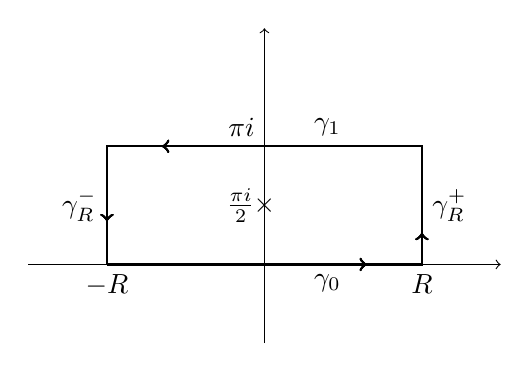
\begin{tikzpicture}
      \draw [->] (-3, 0) -- (3, 0);
      \draw [->] (0, -1) -- (0, 3);

      \draw [black, thick, ->-=0.3, ->-=0.4,->-=0.8,->-=0.95] (-2, 0) node [below] {$-R$} -- (2, 0) node [pos=0.7, below] {$\gamma_0$} node [below] {$R$} -- (2, 1.5) node [pos=0.5, right] {$\gamma_R^+$} -- (-2, 1.5) node [pos=0.3, above] {$\gamma_1$} -- (-2, 0) node [pos=0.5, left] {$\gamma_R^-$};

      \node at (0, 0.75) {$\times$};
      \node [left] at (0, 0.75) {$\frac{\pi i}{2}$};

      \node [circle] at (0, 1.5) {};
      \node [anchor = south east] at (0, 1.5) {$\pi i$};
    \end{tikzpicture}
  \end{center}
As $x=R\rightarrow\pm\infty$, $\cosh z\sim\frac{1}{2}e^{|R|}$. Hence, for $\gamma_R^{\pm}$,
$$\int_{\gamma_R^{\pm}}\sech hzdz=\frac{1}{0.5e^{|R|}}=2e^{-|R|}\rightarrow 0$$
Also, for $\gamma_1$, $z=x+i\pi$ with $x\in[R,-R]$, then
$$\int_{\gamma_1}\sech zdz=\int_{R}^{-R}\frac{2}{e^{i\pi -x}+e^{-i\pi+x}}dx=\int_{-R}^R\frac{2}{e^x+e^{-x}}dx\rightarrow 2I$$
as $R\rightarrow\infty$. Similar for $\gamma_0$, which is much more obvious that this is $2I$ (since $\sech z$ is symmetric about the imaginary axis). Since $\gamma:=\gamma_1\cup\gamma_R^+\cup\gamma_R^-\cup\gamma_0$ is a closed loop, by residue theorem, we must have
$$2\pi i\res_{z=i\pi/2}\sech z=\int_\gamma\sech zdz\rightarrow 4I$$
but LHS is $2\pi i(-i)=2\pi$. Hence, $I=\frac{\pi}{2}$.
\end{ans}
\newpage
\begin{qns}[Choosing contours including keyhole and indentation contours]
Let $a$ be a real non-zero constant. Show that
\begin{enumerate}[label=(\roman*)]
\item 
$$\int_0^\pi\frac{d\theta}{a^2+\sin^2\theta}=\frac{\pi}{a\sqrt{1+a^2}}$$
for $a>1$.
\item 
$$\int_0^\infty\frac{x^4dx}{1+x^8}=\frac{\pi}{4}\sqrt{1-\frac{1}{\sqrt{2}}}$$
\item 
$$\int_0^\infty\cos(0.5ax^2)dx=\sqrt{\frac{\pi}{4|a|}}$$
[Hint: use a sector of a circle with angle $\pi/4$ for (ii) and (iii).] 
\item 
$$\int_0^\infty\frac{x^{-a}dx}{x+1}=\frac{\pi}{\sin(\pi a)}$$
for $0<a<1$;
\item 
$$\int_0^\infty\frac{(\ln x)^2dx}{1+x^2}=\frac{\pi^3}{8}$$
\end{enumerate}
[Hint: (iv) and (v) require you to consider a branch cut; for (v) use a semi-circular contour with an appropriately chosen branch cut.]
\end{qns}
\begin{ans}\leavevmode
\begin{enumerate}[label=(\roman*)]
\item Choose contour $C$ to be a unit circle with $z=e^{i\theta}$ with $\theta\in[0,2\pi)$. Then,
\begin{align}
\int_0^{2\pi}\frac{d\theta}{a^2+\sin^2\theta}&=\oint_C\frac{dz}{iz}\frac{1}{a^2-0.25(z^{-1}-z)^2}\nonumber\\&=\oint_C\frac{4izdz}{(1+2az-z^2)(1-2az-z^2)}\nonumber\\&=\oint_C\frac{4izdz}{(z-a-\sqrt{a^2+1})(z+a-\sqrt{a^2+1})(z-a+\sqrt{a^2+1})(z+a+\sqrt{a^2+1})}\nonumber
\end{align}
The integrand has simple poles at $z=a\pm\sqrt{a^2+1}$ and $z=-a\pm\sqrt{a^2+1}$. But since the $a\in\mathbb{R}$ and $a>1$, then only the poles $z=\pm a\mp\sqrt{a^2+1}$ are enclosed by $C$. The residues at these two poles are
\begin{eqnarray}
&&\res_{z=\pm a\mp\sqrt{a^2+1}}\frac{4iz}{(1+2az-z^2)(1-2az-z^2)}\nonumber\\&=&\res_{z\rightarrow \pm a\mp\sqrt{a^2+1}}\frac{4iz}{(z-a-\sqrt{a^2+1})(z+a+\sqrt{a^2+1})(z\pm a\mp\sqrt{a^2+1})}\nonumber\\&=&\frac{\pm4i(a-\sqrt{a^2+1})}{\pm(-2\sqrt{a^2+1})(2a)(a-\sqrt{a^2+1})}\nonumber\\&=&\frac{-i}{a\sqrt{a^2+1}}\nonumber    
\end{eqnarray}
Since the integrand is symmetric, then $\int_0^{2\pi}\frac{d\theta}{a^2+\sin^2\theta}=2\int_0^\pi\frac{d\theta}{a^2+\sin^2\theta}$, and so by residue theorem,
$$\int_0^\pi\frac{d\theta}{a^2+\sin^2\theta}=\frac{1}{2}\oint_C\frac{d\theta}{a^2+\sin^2\theta}=2\pi i\frac{-2i}{a\sqrt{a^2+1}}=\frac{\pi}{a\sqrt{a^2+1}}$$
 \begin{center}
    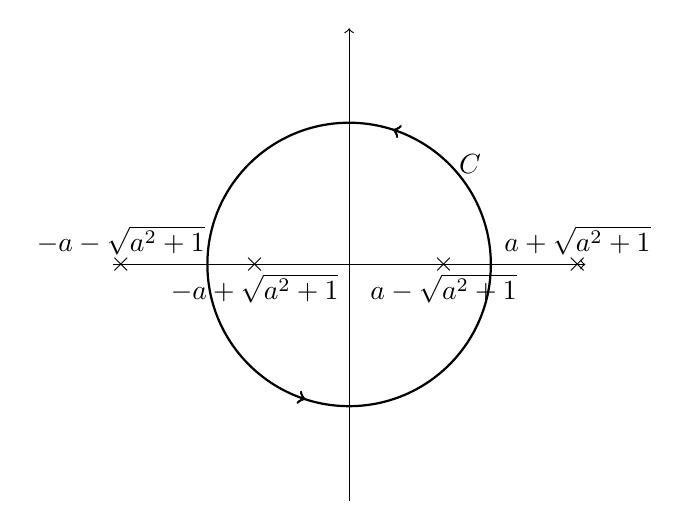
\begin{tikzpicture}
      \draw [->] (-3, 0) -- (3, 0);
      \draw [->] (0, -3) -- (0, 3);
      \draw [black, thick, ->-=0.2,->-=0.7] circle [radius=1.8];
      \node [right] at (1.2726, 1.2726) {$C$};

      \node (z-) at (-2.9, 0) {$\times$};
      \node [above] at (z-) {$-a-\sqrt{a^2+1}$};

      \node (z+) at (-1.2, 0) {$\times$};
      \node [below] at (z+) {$-a+\sqrt{a^2+1}$};
     \node (y-) at (2.9, 0) {$\times$};
      \node [above] at (y-) {$a+\sqrt{a^2+1}$};

      \node (y+) at (1.2, 0) {$\times$};
      \node [below] at (y+) {$a-\sqrt{a^2+1}$};

    \end{tikzpicture}
  \end{center}
\item Let $I=\int_0^\infty\frac{x^4}{1+x^8}dx$ and hence consider $\oint_C\frac{z^4}{1+z^8}dz$. The integrand has 8 simple poles. We choose the contour to be a sector of a circle with angle $\pi/4$ such that only one pole $e^{i\pi/8}$ is enclosed. The residue at this pole is
$$\res_{z=e^{i\pi/8}}\frac{z^4}{1+z^8}=\lim_{z\rightarrow e^{i\pi/8}}\frac{(z-e^{i\pi/8})z^4}{1+z^8}=\lim_{z\rightarrow e^{i\pi/8}}\frac{5z^4-4z^3e^{i\pi/8}}{8z^7}=\frac{1}{8}e^{-i3\pi/8}$$
where we used L'Hopital rule.
 \begin{center}
    \begin{tikzpicture}
      \draw [->] (-3, 0) -- (3, 0);
      \draw [-<-=0.5] (1.41 ,1.41) -- (0,0);
      \draw [->] (0, -3) -- (0, 3);
      \draw [->-=0.5] (0,0) -- (2,0);
      \draw [black,thick,domain=0:45,->-=0.5] plot ({2*cos(\x)}, {2*sin(\x)});
      \node [above] at (0.5, 0.75) {$C_3$};
      \node [below] at (0.35, 0) {$C_1$};
      \node [right] at (1.75, 1.25) {$C_2$};
      \node (z-) at (0.9, 0.5) {$\times$};
      \node [right] at (z-) {$e^{i\pi/8}$};
    \end{tikzpicture}
  \end{center}
Parametrize the curves: 
\begin{itemize}
    \item $C_1$: $z=r$, $r\in[0,R]$
    \item $C_2$: $z=Re^{i\theta}$, $\theta\in[0,\pi/4]$
    \item $C_3$: $z=re^{i\pi/4}$, $r\in[R,0]$.
\end{itemize}
Then, we have the integrals to be
$$\int_{C_1}\frac{z^4}{1+z^8}dz=\int_0^R\frac{r^4}{1+r^8}dr\rightarrow I\text{ as }R\rightarrow\infty$$
$$\int_{C_2}\frac{z^4}{1+z^8}dz=\int_0^{\pi/4}\frac{R^4e^{i\pi}iRe^{i\theta}}{1+R^8e^{i2\pi}}d\theta\sim O(R^{-3})\rightarrow 0\text{ as }R\rightarrow\infty$$
$$\int_{C_3}\frac{z^4}{1+z^8}dz=\int_R^0\frac{r^4e^{i\pi}}{1+r^8e^{i\pi}}e^{i\pi/4}dr\rightarrow e^{i\pi/4} I\text{ as }R\rightarrow\infty$$
Then, by residue theorem:
$$2\pi i\frac{1}{8}e^{-i3\pi/8}=\int_{C_1\cup C_2\cup C_3}\frac{z^4}{1+z^8}dz=I+0+Ie^{i\pi/4}\implies\frac{\pi}{4}=I2\cos\frac{\pi}{8}\implies I=\frac{\pi}{8\cos(\pi/8)}
=\frac{\pi}{8}\sqrt{\frac{2\sqrt{2}}{1+\sqrt{2}}}$$
\item Let $I=\int_0^\infty\cos(0.5ax^2)dx$ and hence consider 
$$\oint_C\cos(0.5az^2)dz=\oint_C\text{Re}[\exp(-|a|z^2/2)]dz$$
where by residue theorem, we get 0 since there is no singularities if we choose $C$ to be the same arc circle as in part (ii):
 \begin{center}
    \begin{tikzpicture}
      \draw [->] (-3, 0) -- (3, 0);
      \draw [-<-=0.5] (1.41 ,1.41) -- (0,0);
      \draw [->] (0, -3) -- (0, 3);
      \draw [->-=0.5] (0,0) -- (2,0);
      \draw [black,thick,domain=0:45,->-=0.5] plot ({2*cos(\x)}, {2*sin(\x)});
      \node [above] at (0.5, 0.75) {$C_3$};
      \node [below] at (0.35, 0) {$C_1$};
      \node [right] at (1.75, 1.25) {$C_2$};
    \end{tikzpicture}
  \end{center}
  Parametrize the curves: 
\begin{itemize}
    \item $C_1$: $z=r$, $r\in[0,R]$
    \item $C_2$: $z=Re^{i\theta}$, $\theta\in[0,\pi/4]$
    \item $C_3$: $z=re^{i\pi/4}$, $r\in[R,0]$.
\end{itemize}
Then, we have the integrals to be
\begin{align}
\int_{C_2}\cos(0.5az^2)dz&=\int_0^{\pi/4}\text{Re}[\exp(i|a|R^2e^{2i\theta}/2)iRe^{i\theta}]d\theta\nonumber\\&=\int_0^{\pi/4}\text{Re}[iRe^{i\theta}\exp(i|a|R^2\cos(2\theta)/2)\exp(-|a|R^2\sin2\theta/2)]d\theta\rightarrow 0\text{ as } R\rightarrow\infty\nonumber
\end{align}
\begin{align}
\int_{C_3}\cos(0.5az^2)dz&=\int_{\infty}^{0}\text{Re}[e^{i\pi/4}\exp(i|a|r^2e^{i\pi/2}/2)]dr\nonumber\\&=-\int_0^\infty\frac{1}{\sqrt{2}}e^{-|a|r^2/2}dr\nonumber\\&=-\frac{1}{\sqrt{2}}\frac{1}{2}\sqrt{\frac{2\pi}{|a|}}=-\sqrt{\frac{\pi}{4|a|}}\nonumber
\end{align}
and last one is obvious. $\int_{C_1}\cos(0.5az^2)dz\rightarrow I$ as $R\rightarrow\infty$ by construction. We then have
$$0=\int_{C_1\cup C_2\cup C_3}\cos(0.5az^2)dz=0+I-\sqrt{\frac{\pi}{4|a|}}\implies I=\sqrt{\frac{\pi}{4|a|}}$$
\newpage
\item Let $I=\int_0^\infty\frac{x^{-a}}{x+1}dx$ and hence consider $\oint_C\frac{z^{-a}}{z+1}dz$. The branch point singularity is at $z=0$ and a simple pole at $z=-1$. Need branch cut for $z^{-a}$. Take this along the positive real axis and choose branch $z^{-a}:=r^{-a} e^{-i\alpha\theta}$, where $0\leq\theta<2\pi$. We need to choose a contour $C$ such that it avoids the branch point singularity and the branch cut. As a result, this takes the form of a keyhole contour as shown:
 \begin{center}
    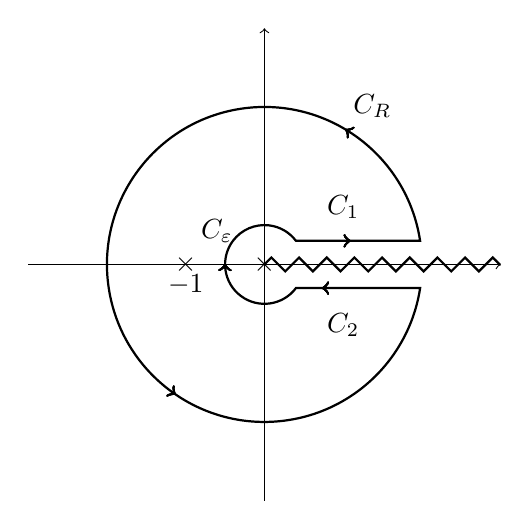
\begin{tikzpicture}
      \draw [->] (-3, 0) -- (3, 0);
      \draw [->] (0, -3) -- (0, 3);
      \draw [thick,decorate, decoration=zigzag] (0, 0) -- (3, 0);

      \draw [black, thick, ->-=0.1, ->-=0.45, ->-=0.75, ->-=0.84, ->-=0.95] (1.977, 0.3) arc(8.63:351.37:2) node [pos=0.15, anchor = south west] {$C_R$} -- (0.4, -0.3) arc(323.13:36.87:0.5) node [pos=0.7, left] {$C_\varepsilon$} -- cycle;
      \node [circle] at (1,1){};
    \node [below] at (1,1){$C_1$};
    \node [circle] at (1,-0.5){};
    \node [below] at (1,-0.5){$C_2$};
      \node [circle] at (0, 0) {};
    \node at (0, 0) {$\times$};
      \node at (-1, 0) {$\times$};
      \node [below] at (-1, 0){$-1$};
    \end{tikzpicture}
  \end{center}
  We could easily see that $\int_{C_R}\frac{z^{-a}}{z+1}dz\sim O(R^{-a})\rightarrow 0$ as $R\rightarrow\infty$ since $0<a<1$. Also, $\int_{C_\varepsilon}\frac{z^{-a}}{z+1}dz\sim O(\varepsilon^{-a+1})\rightarrow 0$ as $\varepsilon\rightarrow 0$ since $0<a<1$.
 For $C_1$:
 $$\int_{\varepsilon}^R\frac{x^{-a}}{x+1}dx\rightarrow I\text{ as }R\rightarrow\infty,~\varepsilon\rightarrow 0$$
 For $C_2$:
  $$\int^{\varepsilon}_R\frac{x^{-a}e^{2\pi ia}}{x+1}dx\rightarrow e^{-2i\pi a}I\text{ as }R\rightarrow\infty,~\varepsilon\rightarrow 0$$
  Only the pole $-1$ is enclosed by the contour, and this residue is
  $$\res_{z=-1}\frac{z^{-a}}{z+1}=\lim_{z\rightarrow -1}z^{-a}=e^{-i\pi a}$$
  By residue theorem,
  $$2\pi ie^{-i\pi a}=\int_{C_1\cup C_2\cup C_{\varepsilon}\cup C_R}\frac{z^{-a}}{z+1}dz=I(1-e^{-2\pi ia})\implies I=\frac{2\pi i}{2i\sin(\pi/a)}$$
\item Let $I=\int_0^\infty\frac{(\ln x)^2}{1+x^2}dx$ and hence consider $\oint_C\frac{(\ln z)^2}{1+z^2}dz$. There is a branch point singularity at $z=0$ and two first order poles at $z=\pm i$. Again, choose a contour that avoids the branch point singularity. Easiest choice is the indentation contour as shown:
 \begin{center}
    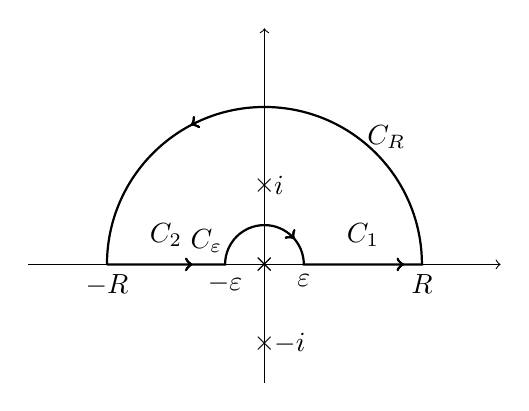
\begin{tikzpicture}
      \draw [->] (-3, 0) -- (3, 0);
      \draw [->] (0, -1.5) -- (0, 3);
      \draw [black, thick, ->-=0.1, ->-=0.25, ->-=0.4, ->-=0.8] (-2, 0) node [below] {$-R$} -- (-0.5, 0) node [below] {$-\varepsilon$} arc(180:0:0.5) node [pos=0.2, left] {$C_\varepsilon$} node [below] {$\varepsilon$} -- (2, 0) node [below] {$R$} arc(0:180:2) node [pos=0.3, right] {$C_R$};
 \node {$\times$};
      \node at (0,1) {$\times$};
      \node [right] at (0, 1) {$i$};
      \node at (0,-1) {$\times$};
      \node [right] at (0, -1) {$-i$};
      
        \node [circle] at (1,1){};
    \node [above] at (1.25,0.1){$C_1$};
    \node [circle] at (1,-1){};
    \node [above] at (-1.25,0.1){$C_2$};
      \node [circle] at (0, 0) {};
    \node at (0, 0) {$\times$};
    \end{tikzpicture}
  \end{center}
We could easily see that as $R\rightarrow\infty$ and $\varepsilon\rightarrow 0$ respectively, we have
$$\int_{C_R}\frac{(\ln z)^2}{1+z^2}dz\sim O(R^{-1})\rightarrow 0,\quad \int_{C_{\varepsilon}}\frac{(\ln z)^2}{1+z^2}dz\sim O(\varepsilon)\rightarrow 0$$
Whereas, we have for $C_1:~z=x,~x\in[\varepsilon,R]$ and $C_2:~z=-x,~x\in[R,\varepsilon]$ respectively: 
$$\int_{\varepsilon}^R\frac{(\ln x)^2}{1+x^2}dx\rightarrow I,\text{ as } R\rightarrow\infty,~\varepsilon\rightarrow 0$$
$$\int^{\varepsilon}_R\frac{(\ln x+i\pi)^2}{1+x^2}dx\rightarrow I+2\pi i\int_0^\infty\frac{\ln x}{1+x^2}dx-\pi^2\int_0^\infty\frac{1}{1+x^2}dx,\text{ as } R\rightarrow\infty,~\varepsilon\rightarrow 0$$
Let $J=\int_0^\infty\frac{\ln x}{1+x^2}dx$ and separately consider $\oint_C\frac{\ln z}{1+z^2}dz$ over the same contour $C$. By a similar argument, $\int_{C_1}\rightarrow J$ and $\int_{C_2}\rightarrow J+i\pi(\pi/2)$. Only the pole $+i$ is enclosed and the residue is
$$\res_{z=i}\frac{(\ln z)}{1+z^2}=\frac{(\ln 1+i0.5\pi)}{i+i}=\frac{\pi}{4}$$
By residue theorem, we must have
$$\oint_C\frac{\ln z}{1+z^2}dz=i\frac{\pi^2}{2}\implies J=\text{Re}[i\pi^2/2]=0$$
Hence, back to evaluating $I$, we have the residue for this case to be instead
$$\res_{z=i}\frac{(\ln z)^2}{1+z^2}=\frac{(\ln 1+i0.5\pi)^2}{i+i}=\frac{i\pi^2}{8}$$
Then by residue theorem,
$$I+I-\frac{\pi^3}{2}=-\frac{\pi^3}{4}\implies I=\frac{\pi^3}{8}$$
\end{enumerate}
\end{ans}
\newpage
\begin{qns}[Branch Cut]
Sketch possible branch cuts for the following complex functions, giving the values on either side of each cut:
\begin{enumerate}[label=(\roman*)]
    \item $(z^2+1)^{0.5}$
    \item $(z^2+1)^{1/3}$
    \item $\ln\bigg[\bigg(\frac{z-i}{z+i}\bigg)^2\bigg]$
\end{enumerate}
\end{qns}
\begin{ans}
There are an unlimited number of possible branch cuts, but we will just discuss the strategy that uses the fewest number of branch cuts.
\begin{enumerate}[label=(\roman*)]
\item $(z^2+1)^{1/2}=(z+i)^{1/2}(z-i)^{1/2}$
Two branch point singularities at $z=\pm i$. We choose the following branch cut with branches $z_1+i=r_1e^{i\theta_1}$, $\theta_1\in[-3\pi/2,\pi/2)$ and $z_2-i=r_2e^{i\theta_2}$, $\theta_2\in[-\pi/2,3\pi/2)$.
\begin{center}
  \begin{tikzpicture}[scale=1.5]
    \draw [->] (-2, 0) -- (2, 0);
    \draw [decorate, thick, decoration=zigzag] (0, -1) -- (0, 1);
    \draw [->] (0, -1) -- (0, 3);
    \node [left] at (0, 1) {$i$};
    \node [left] at (0,-1) {$-i$};
    \node [circle] at (0, 1) {};
    \node [circle] at (0, -1) {};

    \draw (0, -1) -- (2, 2) node [right] {$z$} node [circle] {} node [pos=0.5, anchor = south east] {$r_1$};
    \draw (0, 1) -- (2, 2) node [pos=0.4, anchor = south east] {$r_2$};

    \draw (0, 0.8) arc(-90:8:0.4);
    \node at (0.2, 0.7) [right] {$\theta_2$};

    \draw (0, -0.8) arc (-270:70:0.4);
    \node at (0.5, -1.2) [right] {$\theta_1$};
  \end{tikzpicture}
\end{center}
Say $\theta_1\rightarrow\theta_1+2\pi$, $\theta_2\rightarrow\theta_2$ at $z=-i$, then
$$(z^2+1)^{0.5}\rightarrow\sqrt{r_1r_2}e^{i(\theta_1+\theta_2)/2}e^{i\pi}=-(z^2+1)^{0.5}$$
Say $\theta_1\rightarrow\theta_1$, $\theta_2\rightarrow\theta_2+\pi$ at $z=+i$, then again $(z^2+1)^{0.5}\rightarrow -(z^2+1)^{0.5}$. In another words, if $\theta_1$, $\theta_2$ were to jump individually by $2\pi$, then $(z^2+1)^{0.5}$ is discontinuous. But if both were to jump together by $2\pi$, then $f(z)$ is continuous.
\item 
$(z^2+1)^{1/3}=(z+i)^{1/3}(z-i)^{1/3}$
Again, $z=\pm i$ are branch point singularities. We choose the following branch cut with branches $z_1+i=r_1e^{i\theta_1}$, $\theta_1\in[-\pi/2,3\pi/2)$ and $z_2-i=r_2e^{i\theta_2}$, $\theta_2\in[-3\pi/2,\pi/2)$.
\begin{center}
  \begin{tikzpicture}[scale=1.5]
    \draw [->] (-2, 0) -- (2, 0);
    \draw [decorate, thick, decoration=zigzag] (0, 1) -- (0,2 );
    \draw [decorate, thick, decoration=zigzag] (0, -1) -- (0, -2);
    \draw [->] (0, -1) -- (0, 3);
    \node [left] at (0, 1) {$i$};
    \node [left] at (0,-1) {$-i$};
    \node [circle] at (0, 1) {};
    \node [circle] at (0, -1) {};

    \draw (0, -1) -- (2, 2) node [right] {$z$} node [circle] {} node [pos=0.5, anchor = south east] {$r_1$};
    \draw (0, 1) -- (2, 2) node [pos=0.4, anchor = south east] {$r_2$};

    \draw (0, 1.3) arc(-270:40:0.4);
    \node at (0.2, 0.5) [below] {$\theta_2$};

    \draw (0, -1.2) arc (-90:45:0.4);
    \node at (0.3, -1.2) [right] {$\theta_1$};
  \end{tikzpicture}
\end{center}
Again, this is continuous as long as we don't cross either side of the branch cut.
\item 
$$\ln\bigg(\frac{z-i}{z+i}\bigg)^2=2\ln(z-i)-2\ln(z+i)$$
Same branch point singularities at $z=\pm i$. Let $w=1/z$, then we have $2\ln(1-iw)-2\ln(1+iw)$. $w=0$ is not a branch point singularity, hence $z=\infty$ is not. So, we choose the same branch cut with the same branch as $(z^2+1)^{1/2}$. We then have
$$2\ln\frac{z-i}{z+i}=2\ln(r_1/r_2)+2i(\theta_1-\theta_2)$$
When $\theta_1$ and $\theta_2$ both jump by $2\pi$, $\theta_1-\theta_2$ does not jump. Hence, if the branch cut is not crossed, $\ln\frac{z-i}{z+i}^2$ is continuous.
\end{enumerate}
\end{ans}
\newpage
\subsection*{Transform Methods}
\begin{qns}[Jordan's Lemma]
By considering the integral
$\oint(z^2+1)^{-1}e^{ikz}dz$ taken around a large semicircle, show that for real positive $k$
$$\int_{-\infty}^\infty\frac{\cos(kx)dx}{x^2+1}=\pi e^{-k}$$
What is the value of the integral for $k\leq 0$?
\end{qns}
\begin{ans}
Consider $\oint_C\frac{e^{ikz}}{z^2+1}dz$ where $C=\gamma_R\cup\gamma_0$. We clos the upper half-plane since $k>0$. Since $\frac{1}{z^2+1}\rightarrow 0$ as $|z|\rightarrow\infty$, then by Jordan's Lemma,
$$\int_{\gamma_R}\frac{e^{ikz}}{z^2+1}dz\rightarrow 0,\text{ as }R\rightarrow\infty$$
\begin{center}
    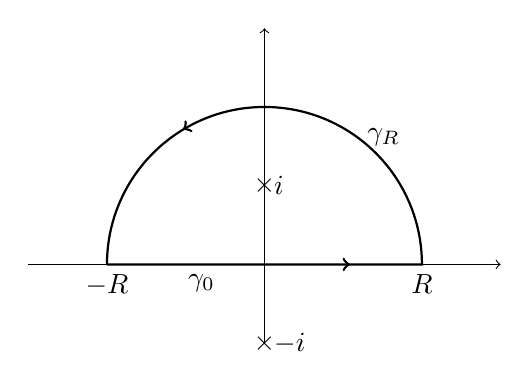
\begin{tikzpicture}
      \draw [->] (-3, 0) -- (3, 0);
      \draw [->] (0, -1) -- (0, 3);

      \draw [black, thick, ->-=0.3, ->-=0.8] (-2, 0) -- (2, 0) node [pos=0.3, below] {$\gamma_0$} arc(0:180:2) node [pos=0.3, right] {$\gamma_R$};

      \node [below] at (-2, 0) {$-R$};
      \node [below] at (2, 0) {$R$};

      \node at (0, 1) {$\times$};
      \node [right] at (0, 1) {$i$};
      \node at (0, -1) {$\times$};
      \node [right] at (0, -1) {$-i$};
    \end{tikzpicture}
  \end{center}
Only one of the two poles of the integrand are enclosed by $C$. The residue at this pole $z=+i$ is
$$\res_{z=i}\frac{e^{ikz}}{z^2+1}=\lim_{z\rightarrow i}\frac{e^{ikz}}{z+i}=\frac{e^{-k}}{2i}$$
The contribution along $\gamma_0$ is
$$\int_{\gamma_0}\frac{e^{ikz}}{z^2+1}dz=\int_{-R}^R\frac{e^{ikz}}{z^2+1}dz\implies\int_{-\infty}^\infty\frac{\cos(kx)dx}{x^2+1}=\lim_{R\rightarrow\infty}\text{Re}\bigg[\int_{-R}^R\frac{e^{ikz}}{z^2+1}dz\bigg]$$
By residue theorem,
$$2\pi i\frac{e^{-k}}{2i}=\int_{-\infty}^\infty\frac{\cos(kx)dx}{x^2+1}\text{ as }R\rightarrow\infty$$
as desired. When $k=0$, we just have $\oint_C\frac{1}{z^2+1}dz$ on the same semi-circle $C$. Using residue theorem again,
$$2\pi i\res_{z=i}\frac{1}{z^2+1}=\int_{\gamma_R}\frac{1}{z^2+1}dz+\int_{-R}^R\frac{1}{z^2+1}dz\leq\frac{\pi R}{R^2+1}+\int_{-R}^R\frac{1}{z^2+1}dz$$
where we used ML inequality. As $R\rightarrow\infty$, RHS approaches $O(R^{-1})+I\rightarrow I$, where $I=\int_{-\infty}^\infty\frac{1}{x^2+1}dx=\pi$. When $k<0$, $\cos(kx)=\cos(|k|x)$, so trivially, the result is $\pi e^{-|k|}$.
\end{ans}
\newpage
\begin{qns}[Inverse Fourier transform]
Find the function $f(x)$ that has Fourier transform $\tilde{f}(k)=(1+k^4)^{-1}$. 
\end{qns}
\begin{ans}
The inverse Fourier transform gives
$$f(x)=\frac{1}{2\pi}\int_{-\infty}^\infty\frac{e^{ikx}}{1+k^4}dk$$
Consider 
$$\frac{1}{2\pi}\oint_{C(x)}\frac{e^{ikx}dk}{(k-e^{i\pi/4})(k-e^{-i\pi/4})(k-e^{3i\pi/4})(k-e^{-3i\pi/4})}$$
where the contour taken $C(x)$ depends on the sign of $x$. If $x>0$, we have $C(x>0)=C_R\cup C_0$ and $C(x<0)=C_R'\cup C_0$ (reason is because of Jordan's Lemma as we will see later) as follow:
\begin{center}
    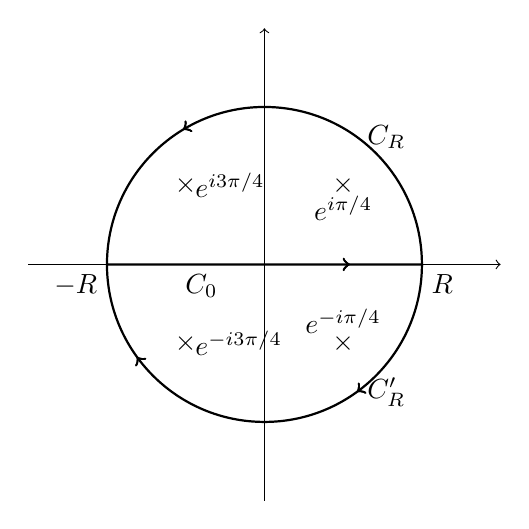
\begin{tikzpicture}
      \draw [->] (-3, 0) -- (3, 0);
      \draw [->] (0, -3) -- (0, 3);

     \draw [black, thick, ->-=0.3, ->-=0.8] (-2, 0) -- (2, 0) node [pos=0.3, below] {$C_0$} arc(0:180:2) node [pos=0.3, right] {$C_R$};
      \draw [black, thick, ->-=0.3, ->-=0.8] (2, 0) arc(0:-180:2) node [pos=0.3, right] {$C_R'$};

      \node [anchor = north east] at (-2, 0) {$-R$};
      \node [anchor = north west] at (2, 0) {$R$};
      \node [circle] at (-2, 0) {};
      \node [circle] at (2, 0) {};

      \node at (1, 1) {$\times$};
      \node [below] at (1, 1) {$e^{i\pi/4}$};
            \node at (1, -1) {$\times$};
      \node [above] at (1, -1) {$e^{-i\pi/4}$};
      \node at (-1, 1) {$\times$};
      \node [right] at (-1, 1) {$e^{i3\pi/4}$};
    \node at (-1, -1) {$\times$};
      \node [right] at (-1, -1) {$e^{-i3\pi/4}$};

    \end{tikzpicture}
  \end{center}
Evidently, as $R\rightarrow\infty$,
$$\frac{1}{2\pi}\int_{C_0}\frac{e^{ikx}dk}{(k-e^{i\pi/4})(k-e^{-i\pi/4})(k-e^{3i\pi/4})(k-e^{-3i\pi/4})}dk\rightarrow I$$
The integrand has poles $k=e^{\pm i\pi/4}=(1\pm i)/\sqrt{2}$ and $e^{\pm i3\pi/4}=(-1\pm i)/\sqrt{2}$. The residues are
\begin{align}
    \res_{k=e^{\pm i\pi/4}}\frac{e^{ikx}}{1+k^4}&=\lim_{k=e^{\pm i\pi/4}}\frac{e^{ikx}}{(k-e^{\mp i\pi/4})(k-e^{3i\pi/4})(k-e^{-3i\pi/4})}\nonumber\\&=\lim_{k=e^{\pm i\pi/4}}\frac{e^{ikx}}{(k-e^{\mp i\pi/4})(k^2-2k\cos(3\pi/4)+1)}\nonumber\\&=\frac{e^{ixe^{\pm i\pi/4}}}{2(1\pm i)(\pm 2i\sin(\pi/4))}\nonumber\\&=-\frac{1}{4}e^{\pm i\pi/4}e^{ix e^{\pm i\pi/4}}\nonumber
\end{align}
\begin{align}
    \res_{k=e^{\pm 3i\pi/4}}\frac{e^{ikx}}{1+k^4}&=\lim_{k=e^{\pm 3i\pi/4}}\frac{e^{ikx}}{(k-e^{\mp i3\pi/4})(k-e^{i\pi/4})(k-e^{-i\pi/4})}\nonumber\\&=\lim_{k=e^{\pm 3i\pi/4}}\frac{e^{ikx}}{(k-e^{\mp 3i\pi/4})(k^2-2k\cos(\pi/4)+1)}\nonumber\\&=\frac{e^{\mp xe^{\pm i\pi/4}}}{2(1\mp i)(\pm 2i\sin(3\pi/4))}\nonumber\\&=\mp\frac{i}{4}e^{\pm i\pi/4}e^{\mp x e^{\pm i\pi/4}}\nonumber
\end{align}
Now for $x>0$, we close the upper half-plane such that we can invoke Jordan's Lemma (since $\frac{1}{1+k^4}\rightarrow 0$ as $|k|\rightarrow\infty$:
$$\int_{C_R}\frac{e^{ikx}}{1+k^4}dk\rightarrow0, \text{ as }R\rightarrow\infty$$
In this case, by residue theorem,
\begin{align}
\oint_{C(x>0)}\frac{e^{ikx}dk}{1+k^4}\frac{1}{2\pi}&=2\pi i\frac{1}{2\pi}\bigg(\res_{z=e^{i\pi/4}}\frac{e^{ikx}}{1+k^4}+\res_{z=e^{3i\pi/4}}\frac{e^{ikx}}{1+k^4}\bigg)\nonumber\\&=-\frac{i}{4}(e^{ixe^{i\pi/4}}+ie^{-xe^{i\pi/4}})e^{i\pi/4}\nonumber\\&=-\frac{i}{4}\frac{1+i}{\sqrt{2}}(e^{ix/\sqrt{2}}e^{-x/\sqrt{2}}+ie^{-x/\sqrt{2}}e^{-ix/\sqrt{2}})\nonumber\\&=\frac{e^{-x/\sqrt{2}}}{2\sqrt{2}}(\cos(x/\sqrt{2})+\sin(x/\sqrt{2}))\nonumber
\end{align}
But LHS $\rightarrow I$ as $R\rightarrow\infty$. Similarly, for $x<0$, we close the lower half-plane such that we can invoke Jordan's Lemma again:
$$\int_{C_R'}\frac{e^{ikx}}{1+k^4}dk\rightarrow0, \text{ as }R\rightarrow\infty$$
In this case, by residue theorem,
\begin{align}
\oint_{C(x<0)}\frac{e^{ikx}dk}{1+k^4}\frac{1}{2\pi}&=2\pi i\frac{1}{2\pi}\bigg(\res_{z=e^{-i\pi/4}}\frac{e^{ikx}}{1+k^4}+\res_{z=e^{-3i\pi/4}}\frac{e^{ikx}}{1+k^4}\bigg)\nonumber\\&=\frac{i}{4}(-e^{ixe^{-i\pi/4}}+ie^{xe^{-i\pi/4}})e^{-i\pi/4}\nonumber\\&=\frac{e^{x/\sqrt{2}}}{2\sqrt{2}}(\cos(x/\sqrt{2})-\sin(x/\sqrt{2}))\nonumber
\end{align}
But LHS $\rightarrow I$ as $R\rightarrow\infty$. Consolidating our results, we have
$$f(x)=\frac{e^{-|x|/\sqrt{2}}}{2\sqrt{2}}(\cos(x/\sqrt{2})+\sin(|x|/\sqrt{2}))$$
which is even as expected from even $\tilde{f}(k)$.
\begin{center}
\begin{tikzpicture}
      \draw[->] (-3,0) -- (3,0) node[right] {$k$};
      \draw[->] (0,0) -- (0,1.5) node[above] {$\tilde{f}(k)$};
      \draw[domain=-3:3,smooth,variable=\x,black] plot ({\x},{1/(1+\x*\x*\x*\x)});
      \draw (0,0) node[below]{0};
    \end{tikzpicture}
\end{center}
\begin{center}
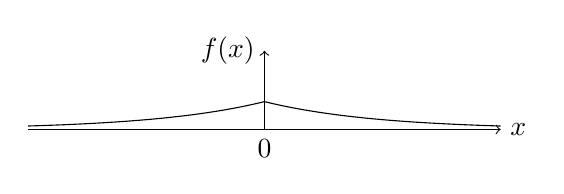
\begin{tikzpicture}
      \draw[->] (-3,0) -- (3,0) node[right] {$x$};
      \draw[->] (0,0) -- (0,1) node[left] {$f(x)$};
      \draw[domain=-3:0,smooth,variable=\x,black] plot ({\x},{(exp(\x/sqrt(2))/(2*sqrt(2)))*(cos(\x/sqrt(2))-sin(\x/sqrt(2)))});
      \draw[domain=0:3,smooth,variable=\x,black] plot ({\x},{(exp(-\x/sqrt(2))/(2*sqrt(2)))*(cos(\x/sqrt(2))+sin(\x/sqrt(2)))});
      \draw (0,0) node[below]{0};
    \end{tikzpicture}
\end{center}
\end{ans}
\newpage
\begin{qns}[Solve PDE]
The motion of an overdamped harmonic oscillator subject to an impulsive force is described by the equation $\ddot{x}+2\gamma\dot{x}+p^2x$ for a function $x(t)$ and constants $\gamma>p>0$. Given that $x = 0$ for $t < 0$, show by Fourier transform methods that for $t > 0$
$$x(t)=\frac{e^{-\gamma t}}{\sqrt{\gamma^2-p^2}}\sinh(\sqrt{\gamma^2-p^2}t)$$
\end{qns}
\begin{ans}
Assume $x(t)$, $\frac{dx}{dt}$ approaches 0 as $|x|\rightarrow\pm\infty$, then the Fourier transform of the PDE is
$$\ddot{x}+2\gamma\dot{x}+p^2x=\delta(t)\implies -k^2\tilde{x}+2\gamma\tilde{x}ik+p^2\tilde{x}=1$$
Hence, using inverse Fourier transform, the solution will be
$$x(t)=\frac{1}{2\pi}\int_{-\infty}^\infty\frac{-e^{ikt}dk}{(k-i(\gamma+\sqrt{\gamma^2-p^2}))(k-i(\gamma-\sqrt{\gamma^2-p^2}))}$$
Since $t>0$, we will close the upper half-plane in order to invoke Jordan's Lemma later. The poles of the integrand are at $k_\pm:=i(\gamma\pm\sqrt{\gamma^2-p^2})$ where $\gamma>p>0$, which are enclosed by the contour when we close the upper-half plane. 
\begin{center}
    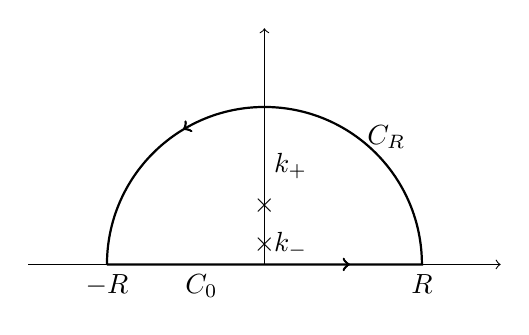
\begin{tikzpicture}
      \draw [->] (-3, 0) -- (3, 0);
      \draw [->] (0, 0) -- (0, 3);

      \draw [black, thick, ->-=0.3, ->-=0.8] (-2, 0) -- (2, 0) node [pos=0.3, below] {$C_0$} arc(0:180:2) node [pos=0.3, right] {$C_R$};

      \node [below] at (-2, 0) {$-R$};
      \node [below] at (2, 0) {$R$};

      \node at (0, 0.75) {$\times$};
      \node [right] at (0, 1.25) {$k_+$};
      \node at (0, 0.25) {$\times$};
      \node [right] at (0, 0.25) {$k_-$};
    \end{tikzpicture}
  \end{center}
The residues are
\begin{align}
\res_{k=i(\gamma\pm\sqrt{\gamma^2-p^2})}\frac{-e^{ikt}}{(k-i(\gamma+\sqrt{\gamma^2-p^2}))(k-i(\gamma-\sqrt{\gamma^2-p^2}))}&=\lim_{k=i(\gamma\pm\sqrt{\gamma^2-p^2})}\frac{-e^{ikt}}{(k-i(\gamma\mp\sqrt{\gamma^2-p^2})}\nonumber\\&=\frac{e^{-(\gamma\pm\sqrt{\gamma^2-p^2})t}}{2i\sqrt{\gamma^2-p^2}}\nonumber
\end{align}
Since $\gamma>0$, by Jordan's Lemma,
$$\int_{C_R}\frac{-e^{-ikt}}{2\pi(k-k_+)(k-k_-)}dk\rightarrow 0,\text{ as }R\rightarrow\infty$$
Evidently,
$$x(t)=\lim_{R\rightarrow\infty}\int_{C_0}\frac{-e^{ikt}}{2\pi(k-k_-)(k-k_+)}dk$$
In this case, by residue theorem,
$$x(t)=\frac{2\pi i}{2i\sqrt{\gamma^2-p^2}}(e^{-(\gamma+\sqrt{\gamma^2-p^2})t}+e^{-(\gamma-\sqrt{\gamma^2-p^2})t})=\frac{e^{-\gamma t}\sinh(\sqrt{\gamma^2-p^2}t)}{\sqrt{\gamma^2-p^2}}$$
as desired. If $t<0$, we close the lower half-plane to use the Jordan's Lemma. In this case, no poles are enclosed and $x(t<0)=0$, consistent with causality.
\end{ans}
\newpage
\begin{qns}[Solve PDE]
A function $u(x,t)$, defined for all $t\geq0$, satisfies the diffusion equation $\frac{\partial u}{\partial t}=\lambda\frac{\partial^2u}{\partial x^2}$ subject to the initial conditions 
$$u(x,0)=
\left\{
        \begin{array}{ll}
      -e^x & x<0 \\
      0 & x=0\\
      e^{-x} & x>0
        \end{array}
    \right.$$
Using Fourier transform methods, show that for $t>0$,
$$u(x,t)=\frac{2}{\pi}\int_0^\infty\frac{ke^{-\lambda k^2t}\sin(kx)}{1+k^2}dk$$
Suppose now that $u(x,t)$ is defined only for $x\geq0$, that $u(0,t)=0$ for all $t\geq0$, and that the initial condition is $u(x,0)=e^{-x}$ for $x > 0$. Write down the solution of this modified problem.
\end{qns}
\begin{ans}
Assume $u$, $\frac{\partial u}{\partial x}\rightarrow 0$ as $|x|\rightarrow\pm\infty$, then the Fourier transform of the diffusion equation gives
$$\frac{\partial\tilde{u}}{\partial t}=-\lambda k^2\tilde{u}\implies\tilde{u}(k,t)=\tilde{u}(k,0)e^{-\lambda k^2t}$$
where the Fourier transform is defined as $\tilde{u}(k,t)=\int_{-\infty}^\infty e^{-ikx}u(x,t)dx$. The transformed initial condition become
$$\tilde{u}(k,0)=\int_{-\infty}^\infty e^{-ikx}u(x,0)dx=-\int_{-\infty}^0e^{-ikx+x}dx+\int_0^\infty e^{-ikx-x}dx=-\frac{1}{1-ik}+\frac{1}{1+ik}=\frac{-2ik}{1+k^2}$$
The solution after inverse Fourier transform becomes
\begin{align}
    u(x,t)&=\frac{1}{2\pi}\int_{-\infty}^\infty\frac{-2ik}{1+k^2}e^{-\lambda k^2t}e^{ikx}dk\nonumber\\&=\frac{2k}{1+k^2}e^{-\lambda k^2t}\sin kxdk\nonumber
\end{align}
where we exploit the even symmetry of the integrand. For the modified problem, $u(0,t)=0\implies\tilde{u}(0,t)=0$ which is consistent with $\tilde{u}(k,t)$ found earlier. The boundary condition is the same for $u(x>0,t)$
\end{ans}
\newpage
\section{Easter Example Sheet 1}
\subsection*{Normal Modes}
\begin{qns}[Normal Modes]
Carefully verify that, in the coupled pendula example (Fig. 1), where each is of length $\ell$, the extension of the spring connecting them is approximately $\ell(\theta_2-\theta_1)$ at . By uniqueness theorem, the solution is the same.leading order in the small angles $\theta_1$ and $\theta_2$.
\begin{figure}[H]
    \centering
    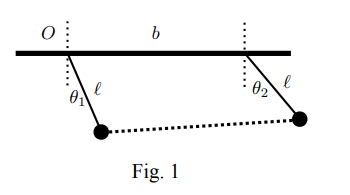
\includegraphics[scale=0.7]{EEx1Q1.PNG}
\end{figure}
\end{qns}
\begin{ans}
The position of particle 1 is $(\ell\sin\theta_1,\ell\cos\theta_1)$ and particle 2 is $(b+\ell\sin\theta_2,\ell\cos\theta_2)$. The length of the spring is
\begin{align}
    b'&=\sqrt{\ell^2(\cos\theta_2-\cos\theta_1)^2+(b+\ell\sin\theta_2-\ell\sin\theta_1)^2}\nonumber\\&=\sqrt{\ell^2(4\sin^2(0.5(\theta_2+\theta_1))\sin^2(0.5(\theta_2-\theta_1))+(b+2\ell\cos(0.5(\theta_2+\theta_1))\sin(0.5(\theta_2-\theta_1)))^2}\nonumber\\&=\sqrt{\ell^2(4\sin^2(0.5(\theta_2-\theta_1)))+(b^2+4b\ell\cos(0.5(\theta_1+\theta_2))\sin(0.5(\theta_2-\theta_1)))}\nonumber\\&=\sqrt{\ell^22\bigg(1-\cos\frac{\theta_2-\theta_1}{2}\bigg)+b^2+4b\ell\cos\frac{\theta_1+\theta_2}{2}\sin\frac{\theta_2-\theta_1}{2}}\nonumber
\end{align}
but $\frac{\theta_2\pm\theta_1}{2}$ is small and assume $b\sim l$ same order. After discarding second order small angle terms,
$$b'\approx\sqrt{b^2+4bl(\frac{\theta_2-\theta_1}{2})}\approx b+2\ell\frac{\theta_2-\theta_1}{2}$$
The extension length will be approximately $b-(b+\ell(\theta_2-\theta_1))=\ell(\theta_2-\theta_1)$.
\end{ans}
\newpage
\begin{qns}[Normal Modes]
Consider a model of a linear molecule AAB where the atom B is at one end. The masses are $M_A=m$, $M_B=2m$ and the spring constants for the forces between neighbouring atoms are given by $k_{AA}=k$, $k_{AB}=2k$. Find the equations of motion and the normal frequencies for linear oscillations along the axis of the molecule. Verify the orthogonality relation for the normal mode vectors $\mathbf{Q}^{(m)}$ and find the normalized form of these generalized eigenvectors.\\[5pt]
At $t = 0$ all atoms are initially at their equilibrium positions, the atoms A are at rest, and atom B is given an initial velocity $u_0$. Derive expressions for the positions of the 3 molecules as functions of $t$, and in terms of the normal modes.
\end{qns}
\begin{ans}
Let $x_1$, $x_2$ and $x_3$ be the displacements from equilibrium, for the three atoms. The kinetic energy is 
$$T=\frac{1}{2}m\dot{x}_1^2+\frac{1}{2}m\dot{x}_2^2+\frac{1}{2}2m\dot{x}_3^2\implies \mathcal{T}=m\begin{pmatrix}1&0&0\\0&1&0\\0&0&2\\\end{pmatrix}$$
The potential energy is
$$V=\frac{1}{2}k(x_2-x_1)^2+\frac{1}{2}(2k)(x_3-x_2)^2=\frac{3}{2}kx_2^2+\frac{1}{2}kx_1^2-k2x_2x_1+kx_3^2-2kx_3x_2\implies \mathcal{V}=k\begin{pmatrix}1&-1&0\\-1&3&-2\\0&-2&2\\\end{pmatrix}$$
Let the normal modes be $x_i(t)=Q_i\sin[\omega(t-t_0)]$, where $t_0$ is determined by initial condition. The Lagrangian is $\mathcal{L}=T-V$ and from Euler-Lagrange equations,
$$0=\frac{d}{dt}\frac{\partial\mathcal{L}}{\partial\dot{x}_i}-\frac{\partial\mathcal{L}}{\partial x_i}=\frac{1}{2}\mathcal{T}_{ij}\ddot{x}_j+\frac{1}{2}\mathcal{V}_{ij}x_j\implies 0=-\omega^2\mathcal{T}_{ij}Q_j+\mathcal{V}_{ij}Q_j$$
For non-trivial $\mathbf{Q}$, we require $\det(-\omega^2\mathcal{T}+\mathcal{V})=0$:
\begin{eqnarray}
0&=&\det\begin{pmatrix}k-\omega^2m&-k&0\\-k&3k-\omega^2m&-2k\\0&-2k&2k-2\omega^2m\end{pmatrix}\nonumber\\&=&(k-\omega^2m)[(3k-\omega^2m)(2k-2\omega^2m)-4k^2]+k(-2k^2+2k\omega^2m)\nonumber\\&=&\omega^2(k-\omega^2m)(\omega^2m-4k)\nonumber
\end{eqnarray}
which suggests $\omega_1^2=0$, $\omega_2^2=\frac{k}{m}$, $\omega_3^2=\frac{4k}{m}$.
$$\omega_1^2=0\implies\begin{pmatrix}k&-k&0\\-k&3k&-2k\\0&-2k&2k\\\end{pmatrix}\mathbf{Q}=\boldsymbol{0}\implies\mathbf{Q}^{(1)}=A_1\begin{pmatrix}1\\1\\1\\\end{pmatrix}$$
$$\omega_2^2=\frac{k}{m}\implies\begin{pmatrix}0&-k&0\\-k&2k&-2k\\0&-2k&0\\\end{pmatrix}\mathbf{Q}=\boldsymbol{0}\implies\mathbf{Q}^{(2)}=A_2\begin{pmatrix}2\\0\\-1\\\end{pmatrix}$$
$$\omega_3^2=\frac{4k}{m}\implies\begin{pmatrix}-3k&-k&0\\-k&-k&-2k\\0&-2k&-6k\\\end{pmatrix}\mathbf{Q}=\boldsymbol{0}\implies\mathbf{Q}^{(3)}=A_3\begin{pmatrix}1\\-3\\1\\\end{pmatrix}$$
To find the normalization constants, we set $(\mathbf{Q}^{(i)})^T\mathcal{T}\mathbf{Q}^{(i)}=1$, then $A_1=\frac{1}{2\sqrt{m}}$, $A_2=\frac{1}{\sqrt{6m}}$, $A_3=\frac{1}{\sqrt{12m}}$. To check orthogonality (with respect to $\mathcal{T}$), compute $(\mathbf{Q}^{(i)})^T\mathcal{T}\mathbf{Q}^{(j)}$ $\forall i,j$. 
$$(\mathbf{Q}^{(1)})^T\mathcal{T}\mathbf{Q}^{(2)}=2-2=0$$
$$(\mathbf{Q}^{(3)})^T\mathcal{T}\mathbf{Q}^{(2)}=2-2=0$$
$$(\mathbf{Q}^{(1)})^T\mathcal{T}\mathbf{Q}^{(3)}=1-3+2=0$$
The general solution will be
$$\mathbf{x}(t)=(c_1+c_2t)\begin{pmatrix}1\\1\\1\\\end{pmatrix}+\text{Re}[c_3e^{i\sqrt{k/m}t}]\begin{pmatrix}2\\0\\-1\\\end{pmatrix}+\text{Re}[c_4e^{i2\sqrt{k/m}t}]\begin{pmatrix}1\\-3\\1\\\end{pmatrix}$$
The initial conditions are $\mathbf{x}(t=0)=\boldsymbol{0}$ and $\mathbf{\dot{x}}(t=0)=(0,0,u_0)^T$.
$$\begin{pmatrix}0\\0\\0\\\end{pmatrix}=c_1\begin{pmatrix}1\\1\\1\\\end{pmatrix}+\text{Re}[c_3]\begin{pmatrix}2\\0\\-1\\\end{pmatrix}+\text{Re}[c_4]\begin{pmatrix}1\\-3\\1\\\end{pmatrix}$$
$$\begin{pmatrix}0\\0\\u_0\\\end{pmatrix}=c_2\begin{pmatrix}1\\1\\1\\\end{pmatrix}+\text{Re}[ic_3]\sqrt{\frac{k}{m}}\begin{pmatrix}2\\0\\-1\\\end{pmatrix}+\text{Re}[ic_4]2\sqrt{\frac{k}{m}}\begin{pmatrix}1\\-3\\1\\\end{pmatrix}$$
We exploit the orthogonality to find the constants.
$$c_1\begin{pmatrix}1&1&1\\\end{pmatrix}\begin{pmatrix}1&0&0\\0&1&0\\0&0&2\\\end{pmatrix}\begin{pmatrix}1\\1\\1\\\end{pmatrix}=\begin{pmatrix}0&0&0\\\end{pmatrix}\begin{pmatrix}1&0&0\\0&1&0\\0&0&2\\\end{pmatrix}\begin{pmatrix}1\\1\\1\\\end{pmatrix}=0$$
$$\text{Re}[c_3]\begin{pmatrix}2&0&-1\\\end{pmatrix}\begin{pmatrix}1&0&0\\0&1&0\\0&0&2\\\end{pmatrix}\begin{pmatrix}1\\1\\1\\\end{pmatrix}=\begin{pmatrix}0&0&0\\\end{pmatrix}\begin{pmatrix}1&0&0\\0&1&0\\0&0&2\\\end{pmatrix}\begin{pmatrix}2\\0\\-1\\\end{pmatrix}=0$$
$$\text{Re}[c_4]\begin{pmatrix}1&-3&1\\\end{pmatrix}\begin{pmatrix}1&0&0\\0&1&0\\0&0&2\\\end{pmatrix}\begin{pmatrix}1\\1\\1\\\end{pmatrix}=\begin{pmatrix}0&0&0\\\end{pmatrix}\begin{pmatrix}1&0&0\\0&1&0\\0&0&2\\\end{pmatrix}\begin{pmatrix}1\\-3\\1\\\end{pmatrix}=0$$
$$c_2\begin{pmatrix}1&1&1\\\end{pmatrix}\begin{pmatrix}1&0&0\\0&1&0\\0&0&2\\\end{pmatrix}\begin{pmatrix}1\\1\\1\\\end{pmatrix}=\begin{pmatrix}0&0&u_0\\\end{pmatrix}\begin{pmatrix}1&0&0\\0&1&0\\0&0&2\\\end{pmatrix}\begin{pmatrix}1\\1\\1\\\end{pmatrix}\implies 4c_2=2u_0$$
$$\text{Re}[ic_3]\sqrt{\frac{k}{m}}\begin{pmatrix}2&0&-1\\\end{pmatrix}\begin{pmatrix}1&0&0\\0&1&0\\0&0&2\\\end{pmatrix}\begin{pmatrix}2\\0\\-1\\\end{pmatrix}=\begin{pmatrix}0&0&u_0\\\end{pmatrix}\begin{pmatrix}1&0&0\\0&1&0\\0&0&2\\\end{pmatrix}\begin{pmatrix}2\\0\\-1\\\end{pmatrix}\implies 6\text{Re}[ic_3]=-2u_0\sqrt{\frac{m}{k}}$$
$$\text{Re}[ic_4]2\sqrt{\frac{k}{m}}\begin{pmatrix}1&-3&1\\\end{pmatrix}\begin{pmatrix}1&0&0\\0&1&0\\0&0&2\\\end{pmatrix}\begin{pmatrix}1\\-3\\1\\\end{pmatrix}=\begin{pmatrix}0&0&u_0\\\end{pmatrix}\begin{pmatrix}1&0&0\\0&1&0\\0&0&2\\\end{pmatrix}\begin{pmatrix}1\\-3\\1\\\end{pmatrix}\implies 12\text{Re}[ic_4]=u_0\sqrt{\frac{m}{k}}$$
Hence,
$$\mathbf{x}(t)=\frac{u_0}{2}t\begin{pmatrix}1\\1\\1\\\end{pmatrix}-\frac{u_0}{3}\sqrt{\frac{m}{k}}\sin\sqrt{\frac{k}{m}}t\begin{pmatrix}2\\0\\-1\\\end{pmatrix}+\frac{u_0}{12}\sqrt{\frac{m}{k}}\sin\sqrt{\frac{4k}{m}}t\begin{pmatrix}1\\-3\\1\\\end{pmatrix}$$
\end{ans}
\newpage
\begin{qns}[Normal Modes]
Three equal masses are connected by equal springs as shown in Fig. 2, the walls being fixed. Assume the motion is constrained to be 1-dimensional along the line of the springs. Find the normal modes of oscillation and the ratios of the normal frequencies. Are there any periodic solutions other than the pure normal modes?
\begin{figure}[H]
    \centering
    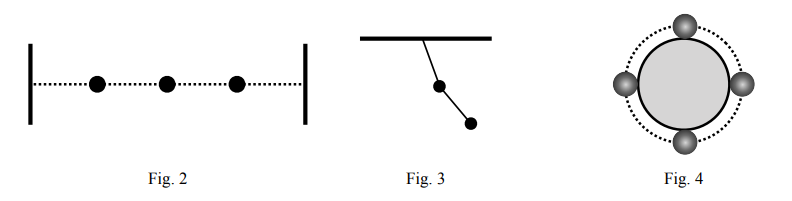
\includegraphics[width=\linewidth]{EEx1Q.PNG}
\end{figure}
\end{qns}
\begin{ans}
Let $x_1$, $x_2$ and $x_3$ be the displacements from equilibrium, for the three atoms. The kinetic energy is 
$$T=\frac{1}{2}m\dot{x}_1^2+\frac{1}{2}m\dot{x}_2^2+\frac{1}{2}m\dot{x}_3^2\implies \mathcal{T}=m\begin{pmatrix}1&0&0\\0&1&0\\0&0&1\\\end{pmatrix}$$
The potential energy is
$$V=\frac{1}{2}kx_1^2+\frac{1}{2}k(x_2-x_1)^2+\frac{1}{2}k(x_3-x_2)^2+\frac{1}{2}k(-x_3)^2\implies \mathcal{V}=k\begin{pmatrix}2&-1&0\\-1&2&-1\\0&-1&2\\\end{pmatrix}$$
Let the normal modes be $x_i(t)=Q_i\sin[\omega(t-t_0)]$, where $t_0$ is determined by initial condition. The Lagrangian is $\mathcal{L}=T-V$ and from Euler-Lagrange equations,
$$0=\frac{d}{dt}\frac{\partial\mathcal{L}}{\partial\dot{x}_i}-\frac{\partial\mathcal{L}}{\partial x_i}=\frac{1}{2}\mathcal{T}_{ij}\ddot{x}_j+\frac{1}{2}\mathcal{V}_{ij}x_j\implies 0=-\omega^2\mathcal{T}_{ij}Q_j+\mathcal{V}_{ij}Q_j$$
For non-trivial $\mathbf{Q}$, we require $\det(-\omega^2\mathcal{T}+\mathcal{V})=0$:
\begin{eqnarray}
0&=&\det\begin{pmatrix}2k-\omega^2m&-k&0\\-k&2k-\omega^2m&-k\\0&-k&2k-2\omega^2m\end{pmatrix}\nonumber\\&=&(2k-\omega^2m)[(2k-\omega^2m)^2-k^2]-k^2(2k-\omega^2m)\nonumber\\&=&(2k-m\omega^2)((2+\sqrt{2})k-m\omega^2)((2-\sqrt{2})k-m\omega^2)\nonumber
\end{eqnarray}
which suggests $\omega_1^2=\frac{2k}{m}$, $\omega_2^2=(2+\sqrt{2})\frac{k}{m}$ and $\omega_3^2=(2-\sqrt{2})\frac{k}{m}$.
$$\omega_1^2=\frac{2k}{m}\implies\begin{pmatrix}0&-k&0\\-k&0&-k\\0&-k&0\\\end{pmatrix}\mathbf{Q}=\boldsymbol{0}\implies\mathbf{Q}^{(1)}=A_1\begin{pmatrix}1\\0\\-1\\\end{pmatrix}$$
$$\omega_2^2=(2+\sqrt{2})\frac{k}{m}\implies\begin{pmatrix}-\sqrt{2}k&-k&0\\-k&-\sqrt{2}k&-k\\0&-k&-\sqrt{2}k\\\end{pmatrix}\mathbf{Q}=\boldsymbol{0}\implies\mathbf{Q}^{(2)}=A_2\begin{pmatrix}1\\-\sqrt{2}\\1\\\end{pmatrix}$$
$$\omega_3^2=(2-\sqrt{2})\frac{k}{m}\implies\begin{pmatrix}\sqrt{2}k&-k&0\\-k&\sqrt{2}k&-k\\0&-k&\sqrt{2}k\\\end{pmatrix}\mathbf{Q}=\boldsymbol{0}\implies\mathbf{Q}^{(3)}=A_3\begin{pmatrix}1\\\sqrt{2}\\1\\\end{pmatrix}$$
Since $\mathcal{T}$ is a multiple of the identity matrix, the normalization constant can be found normally, $Q^TQ=1$, so $A_1=\frac{1}{\sqrt{2m}}$, $A_2=\frac{1}{2\sqrt{m}}$ and $A_3=\frac{1}{2\sqrt{m}}$. The three normal modes are
$$\mathbf{x_1}(t)=\frac{1}{\sqrt{2m}}\begin{pmatrix}1\\0\\-1\\\end{pmatrix}\sin\sqrt{\frac{2k}{m}}(t-t_0)$$
$$\mathbf{x_2}(t)=\frac{1}{2\sqrt{m}}\begin{pmatrix}1\\-\sqrt{2}\\1\\\end{pmatrix}\sin\sqrt{\frac{(2+\sqrt{2})k}{m}}(t-t_0)$$
$$\mathbf{x_3}(t)=\frac{1}{2\sqrt{m}}\begin{pmatrix}1\\\sqrt{2}\\1\\\end{pmatrix}\sin\sqrt{(2-\sqrt{2})\frac{k}{m}}(t-t_0)$$
The ratios of the normal frequencies are $\sqrt{2}$ to $\sqrt{2+\sqrt{2}}$ to $\sqrt{2-\sqrt{2}}$. They might be able to oscillate at different frequencies (not periodic since the ratio of frequencies are not rational).
\end{ans}
\begin{qns}[Normal Modes]
Consider the double pendulum shown in Fig. 3, with two balls of equal mass $m$ at the ends of identical rods, length $\ell$,  whose masses can be neglected. The motion
is constrained to be in a fixed vertical plane. Find the two normal modes of small oscillations and their frequencies. [Hint: Instead of using Newton’s second law, it is easier to determine the kinetic and potential energies and then use Lagrange’s equations.]
\end{qns}
\begin{ans}
The potential energy is
$$V=mg\ell(1-\cos\theta_1)+mg\ell(1-\cos\theta_1+1-\cos\theta_2)\approx mg\ell\theta_1^2+\frac{1}{2}mg\ell\theta_2^2\implies \mathcal{V}=mg\ell\begin{pmatrix}2&0\\0&1\\\end{pmatrix}$$
The kinetic energy is
\begin{eqnarray}
T&=&\frac{1}{2}m[(\ell\dot{\theta}_1\cos\theta_1)^2+(-\ell\dot{\theta}_1\sin\theta_1)^2]+\frac{1}{2}m[(\ell\dot{\theta}_1\cos\theta_1+\ell\dot{\theta}_2\cos\theta_2)^2+(-\ell\dot{\theta}_1\sin\theta_1-\ell\dot{\theta}_2\sin\theta_2)^2]\nonumber\\&=&\frac{1}{2}m\ell^2\dot{\theta}_1^2+\frac{1}{2}m\ell^2\dot{\theta}_1^2+m\ell^2(\cos\theta_1\cos\theta_2+\sin\theta_1\sin\theta_2)\dot{\theta}_1\dot{\theta}_2+\frac{1}{2}m\ell^2\dot{\theta}_2^2\nonumber\\&\approx&m\ell^2\dot{\theta}_1^2+\frac{1}{2}m\ell^2\dot{\theta}_2^2+m\ell^2\dot{\theta}_1\dot{\theta}_2\nonumber\\\implies \mathcal{T}&=&m\ell^2\begin{pmatrix}2&1\\1&1\\\end{pmatrix}\nonumber
\end{eqnarray}
The Euler-Lagrange equations give $\mathcal{L}=T-V\implies 0=\frac{d}{dt}\frac{\partial\mathcal{L}}{\partial\dot{\theta}_i}-\frac{\partial\mathcal{L}}{\partial\theta_i}=\mathcal{T}_{ij}\ddot{\theta}_j+\mathcal{V}_{ij}\theta_j$. For normal modes $\theta_i(t)=Q_i\sin[\omega(t-t_0)]$ where $t_0$ is determined by initial condition, we have $(-\omega^2T+V)\mathbf{Q}=\boldsymbol{0}$. For non-trivial solutions, we require $\det(-\omega^2\mathcal{T}+\mathcal{V})=0$:
$$0=\det\begin{pmatrix}2g-2\ell\omega^2&-\ell\omega^2\\-\ell\omega^2&g-\ell\omega^2\\\end{pmatrix}=2(g-\ell\omega^2)(g-\ell\omega^2)-\ell^2\omega^4$$
which gives $\omega_1^2=\frac{\sqrt{2}}{\sqrt{2}+1}\frac{g}{\ell}$, $\omega_2^2=\frac{\sqrt{2}}{\sqrt{2}-1}\frac{g}{\ell}$.
$$\omega_1^2=\frac{\sqrt{2}}{\sqrt{2}+1}\frac{g}{\ell}\implies\begin{pmatrix}2&-\sqrt{2}\\-\sqrt{2}&1\\\end{pmatrix}\mathbf{Q}=\boldsymbol{0}\implies\mathbf{Q}^{(1)}=A_1\begin{pmatrix}1\\\sqrt{2}\\\end{pmatrix}$$
$$\omega_2^2=\frac{\sqrt{2}}{\sqrt{2}-1}\frac{g}{\ell}\implies\begin{pmatrix}2&\sqrt{2}\\\sqrt{2}&1\\\end{pmatrix}\mathbf{Q}=\boldsymbol{0}\implies\mathbf{Q}^{(2)}=A_2\begin{pmatrix}1\\-\sqrt{2}\\\end{pmatrix}$$
To find the normalization constants, we set $(\mathbf{Q}^{(i)})^T\mathcal{T}\mathbf{Q}^{(i)}=1$, then $A_1=\frac{1}{\sqrt{(4+2\sqrt{2})m\ell^2}}$, $A_2=\frac{1}{\sqrt{(4-2\sqrt{2})m\ell^2}}$. The two normal modes are
$$\boldsymbol{\theta}^{(1)}=\frac{1}{\sqrt{(4+2\sqrt{2})m\ell^2}}\begin{pmatrix}1\\\sqrt{2}\\\end{pmatrix}\sin\sqrt{\frac{\sqrt{2}}{\sqrt{2}+1}}\sqrt{\frac{g}{\ell}}(t-t_0)$$
$$\boldsymbol{\theta}^{(2)}=\frac{1}{\sqrt{(4-2\sqrt{2})m\ell^2}}\begin{pmatrix}1\\-\sqrt{2}\\\end{pmatrix}\sin\sqrt{\frac{\sqrt{2}}{\sqrt{2}-1}}\sqrt{\frac{g}{\ell}}(t-t_0)$$
\end{ans}
\newpage
\begin{qns}[Normal Modes]
Four point-size beads of mass m are constrained to move on a frictionless circle of radius R (Fig. 4). Adjacent pairs of beads are connected by springs of spring constant and equilibrium length $\frac{\pi R}{2}$. Write down the Lagrangian for the system. Find the normal modes and normal frequencies. Describe the motions corresponding to each normal mode.
\end{qns}
\begin{ans}
The kinetic energy is
$$T=\frac{1}{2}m\dot{x}_1^2+\frac{1}{2}m\dot{x}_2^2+\frac{1}{2}m\dot{x}_3^2+\frac{1}{2}m\dot{x}_4^2\implies \mathcal{T}=m\diag(1,1,1,1)$$
$$V=\frac{1}{2}k(x_2-x_1)^2+\frac{1}{2}k(x_3-x_2)^2+\frac{1}{2}k(x_4-x_3)^2+\frac{1}{2}k(x_1-x_4)^2\implies\mathcal{V}=k\begin{pmatrix}2&-1&0&-1\\-1&2&-1&0\\0&-1&2&-1\\-1&0&-1&2\\\end{pmatrix}$$
Let the normal modes be $x_i(t)=Q_i\sin[\omega(t-t_0)]$, where $t_0$ is determined by initial condition. The Lagrangian is $\mathcal{L}=T-V$ and from Euler-Lagrange equations,
$$0=\frac{d}{dt}\frac{\partial\mathcal{L}}{\partial\dot{x}_i}-\frac{\partial\mathcal{L}}{\partial x_i}=\frac{1}{2}\mathcal{T}_{ij}\ddot{x}_j+\frac{1}{2}\mathcal{V}_{ij}x_j\implies 0=-\omega^2\mathcal{T}_{ij}Q_j+\mathcal{V}_{ij}Q_j$$
For non-trivial $\mathbf{Q}$, we require $\det(-\omega^2\mathcal{T}+\mathcal{V})=0$:
\begin{eqnarray}
0&=&\det\begin{pmatrix}2k-\omega^2m&-k&0&-k\\-k&2k-\omega^2m&-k&0\\0&-k&2k-\omega^2m&-k\\-k&0&-k&2k-\omega^2m\\\end{pmatrix}\nonumber\\&=&(4k-m\omega^2)(2k-m\omega^2)^2\omega^2\nonumber
\end{eqnarray}
which suggests $\omega_1^2=\frac{4k}{m}$, $\omega_2^2=\frac{2k}{m}=\omega_3^2$, $\omega_4^2=0$.
$$\omega_1^2=\frac{4k}{m}\implies\mathbf{Q}^{(1)}=A_1\begin{pmatrix}-1\\1\\-1\\1\\\end{pmatrix}$$
$$\omega_2^2=\frac{2k}{m}\implies\mathbf{Q}^{(2)}=A_2\begin{pmatrix}0\\-1\\0\\1\\\end{pmatrix},\quad \mathbf{Q}^{(3)}=A_3\begin{pmatrix}-1\\0\\1\\0\\\end{pmatrix}$$
$$\omega_4^2=0\implies\mathbf{Q}^{(4)}=A_4\begin{pmatrix}1\\1\\1\\1\\\end{pmatrix}$$
The first normal mode is the adjacent masses in anti-phase with equal amplitudes, second and third ones would be the anti-podal masses fixed, and the other two in anti-phase with equal amplitudes. Finally, the fourth one corresponds to the trivial rigid body rotation.
\end{ans}
\begin{qns}[Lagrangian]
Let $T=\frac{1}{2}T_{ij}\dot{q}_i\dot{q}_j$ and $V=\frac{1}{2}V_{ij}q_iq_j$. Verify that the equations of motion $T_{ij}\ddot{q}_j+V_{ij}q_j=0$ imply that the energy $T +V$ is conserved. Can the constancy of $T +V$ be used to deduce the equations of motion?
\end{qns}
\begin{ans}
Take $\mathcal{L}=T-V$, use Euler-Lagrange equations to obtain the equations of motion 
\begin{equation}
    T_{ij}\ddot{q}_j+V_{ij}q_j=0\tag{*}
\end{equation}
Take (*) multiply with $\dot{q}_i$. Swap the index $i$ and $j$ for the result, and add both together, to get
\begin{equation}
    0=T_{ij}\dot{q}_j\ddot{q}_j+T_{ij}\ddot{q}_i\dot{q}_j+V_{ij}\dot{q}_iq_j+V_{ij}q_i\dot{q}_j\tag{\dag}
\end{equation}
which is $\frac{d}{dt}2(T+V)$, which suggests $T+V$ is a constant. The converse is not true and we can only prove until (\dag), but not obtain the equations of motion. Specifically, take
$$\frac{dE}{dt}=\mathbf{\dot{q}}\cdot(T\mathbf{\ddot{q}}+V\mathbf{q})=0$$
which suggests either $\mathbf{\dot{q}}=\boldsymbol{0}$, or $\mathbf{\dot{q}}\perp(T\mathbf{\ddot{q}}+V\mathbf{q})$ or the equations of motion.
\end{ans}
\newpage
\subsection*{Group Theory}
\begin{qns}[Functions, M\"{o}bius group]
The six functions $f_1,f_2,\dots,f_6$ are defined by
$$f_1(z)=z;\quad f_2(z)=(1-z)^{-1};\quad f_3(z)=1-z^{-1};$$
$$f_4(z)=z^{-1};\quad f_5(z)=1-z;\quad f_6(z)=z(z-1)^{-1}$$
Show that these functions form a group under function composition, i.e., ‘function of a function’: the ‘product’ $f_1f_2$ being defined by $f_1f_2(z):=f_1(f_2(z))$. Construct the group table, find all subgroups, and determine which of them are normal. (There are three order-2 subgroups none of which is normal, and one order-3 subgroup, which is normal.) Is this group isomorphic to any other group mentioned in the lectures? What happens to the points $z=0,1,\infty$ for each of the functions $f_1,f_2,\dots,f_6$?
\end{qns}
\begin{ans}
We demonstrate $\{f_1,f_2,f_3,f_4,f_5,f_6\}$ is a group under function composition. Evidently, operation with $f_1$ is commutative.
$$f_1\circ f_1=f_1;\quad f_2\circ f_1=f_2; f_3\circ f_1=f_3;\quad f_4\circ f_1=f_4;\quad f_5\circ f_1=f_5;\quad f_6\circ f_1=f_6$$
We proceed with $f_2$ first:
$$f_2\circ f_2=\frac{1}{1-(1-z)^{-1}}=1-z^{-1}=f_3;\quad f_3\circ f_2=(1-(1-z^{-1}))^{-1}=z=f_1;\quad f_4\circ f_2=(1-z)=f_5;...$$
$$f_5\circ f_2=1-(1-z)^{-1}=\frac{-z}{1-z}=f_6;\quad f_6\circ f_2=(1-z)^{-1}((1-z)^{-1}-1)^{-1}=f_4$$
then $f_3$:
$$f_3\circ f_3=1-(1-z^{-1})^{-1}=(1-z)^{-1}=f_2;\quad f_2\circ f_3=f_1;\quad f_4\circ f_3=(1-z^{-1})^{-1}=f_6;...$$
$$f_5\circ f_3=1-(1-z^{-1})=f_4;\quad f_6\circ f_3=(1-z^{-1}))(1-z^{-1}-1)^{-1}=1-z=f_5$$
then $f_4$:
$$f_4\circ f_4=z=f_1;\quad f_2\circ f_4=(1-z^{-1})^{-1}=z(z-1)^{-1}=f_6;\quad f_3\circ f_4=1-z=f_5;...$$
$$f_5\circ f_4=1-z^{-1}=f_3;\quad f_6\circ f_4=z^{-1}(z^{-1}-1)^{-1}=(1-z)^{-1}=f_2$$
then $f_5$:
$$f_5\circ f_5=1-(1-z)=z=f_1;\quad f_2\circ f_5=(1-1+z))^{-1}=f_4;\quad f_3\circ f_5=1-(1-z)^{-1}=z(z-1)^{-1}=f_6;...$$
$$f_4\circ f_5=f_2;\quad f_6\circ f_5=(1-z)z^{-1}=1-z^{-1}=f_3$$
lastly, $f_6$:
$$f_6\circ f_6=z(z-1)^{-1}(z(z-1)^{-1}-1)^{-1}=z=f_1;\quad f_2\circ f_6=(1-z(z-1)^{-1})^{-1}=f_5;...$$
$$f_3\circ f_6=1-z^{-1}(z-1)=z^{-1}=f_4;\quad f_4\circ f_6=z^{-1}(z-1)=f_3;\quad f_5\circ f_6=1-z(z-1)^{-1}=(1-z)^{-1}=f_2$$
The group table is thus
$$\vbox{\tabskip0.5em\offinterlineskip
    \halign{\strut$#$\hfil\ \tabskip1em\vrule&&$#$\hfil\cr
    ~   & f_1   & f_2   & f_3 & f_4 & f_5 & f_6     \cr
    \noalign{\hrule}\vrule height 12pt width 0pt
    f_1   & f_1   & f_2  & f_3 & f_4 & f_5 & f_6      \cr
    f_2   & f_2  &f_3   & f_1 & f_6   & f_4 & f_5      \cr
    f_3 & f_3 & f_1   & f_2   & f_5 & f_4 & f_6      \cr
    f_4   & f_4   & f_5   & f_6   & f_1 & f_2 & f_3     \cr
    f_5   & f_5   & f_6   & f_4   & f_3 & f_1 & f_2     \cr
    f_6   & f_6   & f_4   &  f_5  & f_2 & f_3 & f_1     \cr
}}$$
Observe the diagonal elements of the group table, to find the subgroups to be
\begin{itemize}
    \item $\{f_1,f_4\}$
    \item $\{f_1,f_5\}$
    \item $\{f_1,f_6\}$
    \item $\{f_1,f_2,f_3\}$
\end{itemize}
We check that these sets satisfy the group axioms with $f_1$ being identity and function composition as the binary operation:\\[5pt]
For all, associativity is inherited from the parent group $\{f_1,f_2,f_3,f_4,f_5,f_6\}$. For the first three: They are definitely closed ($f_i\circ f_1=f_1\circ f_i=f_i$ and $f_i\circ f_i=f_1\circ f_1=f_1$), with $f_1$ being the identity and $f_i=f_4, f_5, f_6$ is its own inverse. For the last one, it is closed ($f_1\circ f_2=f_3\circ f_3=f_2$ and $f_1\circ f_3=f_2\circ f_2=f_3$ and $f_2\circ f_3=f_1\circ f_1=f_1$), with $f_1$ being the identity and $f_2$ is $f_3$'s inverse, and vice-versa.\\[5pt]
The first three isn't normal since we can't find a $f$ in the group such that $ff_1f^{-1}=f_i$. The last one is normal, consisting of conjugacy classes $\{f_1\}$ and $\{f_2,f_3\}$, since $f_2f_3=f_1$, i.e. $f_3$ and $f_2$ are inverses of each other. Hence, $$f_3^{-1}f_2f_3=f_2f_2f_3=f_2f_1=f_2$$ $$f_2^{-1}f_3f_2=f_3f_3f_2=f_3f_1=f_3$$
The group is isomorphic to the dihedral group $D_3=\{I,R,R^2,m_1,m_2,m_3\}$ such that one can construct a bijective map $\Phi$ such that $I\mapsto f_1$, $R\mapsto f_2$, $R^2\mapsto f_3$, $m_1\mapsto f_4$, $m_3\mapsto f_5$, $m_2\mapsto f_6$.\\[5pt]
In fact, $f_i$ is a M\"{o}bius map of the generic form $f_i(z)=\frac{az+b}{cz+d}$, where $a,b,c,d\in\mathbb{C}$, which solely compose of dilation, translation and inversion. Here, we define the extended complex plane to be $\hat{\mathbb{C}}=\mathbb{C}\cup\{0\}$ but $\pm\infty$ is in fact the same point in this extended complex plane. They are all distinct since each $f_i$ take the triplet $(0,1,\infty)$ into a distinct triplet in $\hat{\mathbb{C}}$.
\begin{center}
\begin{tabular}{ |c|c|c|c| } 
\hline
    $z=$&0&1&$\infty$\\
 \hline
 $f_1$ & 0 & 1 & $\infty$ \\ 
 $f_2$ & 1 & $\infty$ & 0 \\
 $f_3$ & $\infty$ & 0 &1\\
 $f_4$ & $\infty$ & 1 & 0\\
 $f_5$ & 1 & 0 &$\infty$\\
 $f_6$& 0 &$\infty$&1\\
 \hline
\end{tabular}
\end{center}
\end{ans}
\begin{qns}[Group Table, Isomorphism]
Find the group table for the cyclic group $C_4$ , consisting of rotations in a plane by angles $\frac{n\pi}{2}$, where $n = 0, 1, 2,$ or $3$. Find the group table for the so-called Vierergruppe $V$ (also referred to as Klein’s four-group and denoted $K_4$), consisting of the identity and the rotations by $\pi$ about the $x$, $y$, and $z$ axes in 3-dimensional space. Show that both $C_4$ and $V$ are Abelian, but that they are not isomorphic to each other
\end{qns}
\begin{ans}
$C_4=\{I,R,R^2,R^3\}$, and the group table is
$$\vbox{\tabskip0.5em\offinterlineskip
    \halign{\strut$#$\hfil\ \tabskip1em\vrule&&$#$\hfil\cr
    ~   & I   & R   & R^2 & R^3     \cr
    \noalign{\hrule}\vrule height 12pt width 0pt
    I   & I   & R  & R^2 & R^3      \cr
    R   & R   & R^2 & R^3   & I      \cr
    R^2 & R^2 & R^3   & I   & R      \cr
    R^3   & R^3   & I   & R   & R^2     \cr
}}$$
Since $g_1g_2=g_2g_1$ $\forall g_1,g_2\in C_4$, $C_4$ is an abelian group. $V=\{I,R^x,R^y,R^z\}$ where $R^i$ is a single rotation by $\pi$ radians about the $i$-axis. The group table is
$$\vbox{\tabskip0.5em\offinterlineskip
    \halign{\strut$#$\hfil\ \tabskip1em\vrule&&$#$\hfil\cr
    ~   & I   & R^x   & R^y & R^z     \cr
    \noalign{\hrule}\vrule height 12pt width 0pt
    I   & I   & R^x  & R^y & R^z      \cr
    R^x   & R^x   & I & R^z   & R^y      \cr
    R^y & R^y & R^z   & I   & R^x     \cr
    R^z   & R^z   & R^y   & R^x   & I     \cr
}}$$
Likewise, $V$ is abelian. We have $RR\neq I$, so the order of $R$ is not two. This is unlike $R^iR^i=I$ $\forall i$ so the order of $R^i$ is two. The structural difference suggests that $C^4$ and $V$ are not isomorphic.
\end{ans}
\begin{qns}[Dihedral Group]
The symmetry group of an $N$-gon is generated by a single rotation by $2\pi/N$, denoted $R$, and a reflection $m$ (being any single one of the possible reflectional symmetries). Show by means of sketches that the relations $R^N=I$ , $m^2=I$ and $Rm=mR^{-1}$ are always obeyed. Deduce that the elements of the group are $R^n$ and $R^nm$ where $n\in\{1,2,...,N\}$. Use the foregoing relations to express the product of two arbitrary elements of the group either in
the form $R^n$ or in the form $R^nm$.
\end{qns}
\begin{ans}
Consider two adjacent points on the $N$-gon. Let them be $X$ and $X'$. The interior angle is $\frac{2\pi}{N}$ and so the two points are separated by this angle. $R$ maps $X$ to $X'$, and so $R^N$ will lead to one complete rotation, i.e. $2\pi$ radians, and so $R^N=I$.\\[5pt]
Separately, consider two arbitrary points $X$ and $X'$ which are related to each other by a reflection plane, and the angle between the two points is $2\theta$. The reflection $m$ maps $X$ to $X'$ and $m^2$ maps $X'$ back to $X$, so $m^2=I$.\\[5pt]
Finally, consider four points $X$, $X'$, $X''$ and $X'''$. $X$ and $X'$ are related by a plane of symmetry, while $X'$ and $X''$, and $X'''$ and $X$, are each separated by angle $\frac{2\pi}{N}$. We have $Rm: X\mapsto X''$ and $mR^{-1}:X\mapsto X''$ and so $Rm=mR^{-1}$.\\[5pt]
Since $N$-gon is invariant under rotations by multiples of $\frac{2\pi}{N}$, $R^n$ where $1\leq n\leq N$ are elements of this symmetry group. There are $N$ planes of reflection so $m_n$ where $1\leq n\leq N$ are group elements. However, $m_n$ where $n\geq2$ can be generated from a combination of $m_1$ and $R$, then $m_n=R^nm_1$. So the group elements are $R^n$ and $R^nm_1$, where $1\leq n\leq N$.\\[5pt]
Product of any two arbitrary elements: 
$$R^jR^i=R^{(i+j)\mod N}$$
$$R^jR^im=R^{(i+j)\mod N}m$$
$$R^jmR^i=R^jmR^{-1}R^{i+1}=R^jRmR^{i+1}=R^{j+1}mR^{i+1}=R^{j-i}m$$
$$R^jmR^im=R^{j-i}$$
\end{ans}
\begin{qns}[Permutation]
Show that the order of a permutation $P$ is the lowest common multiple of the orders of its component cycles. Resolve
$$P=\begin{pmatrix}1&2&3&4&5&6&7&8&9\\4&6&9&7&2&5&8&1&3\\\end{pmatrix}$$
into cycles and find its order.
\end{qns}
\begin{ans}
Every permutation in $S_n$ is a composition of disjoint cycles. The expression of an element $\sigma\in S_n$ as a composition of disjoint cycles
$$\sigma=(a_1^1a_2^1\dots a_{k_1}^1)(a_1^2a_2^2\dots a_{k_2}^2)\dots(a_1^ra_2^r\dots a_{k_r}^r)$$
We want to show the order of $\sigma$ is the lowest common multiple of the $k_i$'s: Evaluate $\sigma^j$
$$\sigma^j=(a_1^1a_2^1\dots a_{k_1}^1)^j(a_1^2a_2^2\dots a_{k_2}^2)^j\dots(a_1^ra_2^r\dots a_{k_r}^r)^j$$
as disjoint cycles commute with each other. Since the order of a cycle $(b_1b_2\dots b_r)$ is $r$, then when $l:=\lcm\{k_i\}$, we have
$$(a_1^ia_2^i\dots a_{k_i}^i)^l=((a_1^ia_2^i\dots a_{k_i}^i)^{k_i})^{l/k_i}=e^{l/k_i}=e$$
and so the order of $\sigma$ divides $l$. On the other hand, if $\sigma$ has order $m$, then rearranging, we have
$$(a_1^1a_2^1\dots a_{k_1}^1)^m=((a_1^2a_2^2\dots a_{k_2}^2)^m\dots(a_1^ra_2^r\dots a_{k_r}^r)^m)^{-1}$$
but the LHS fixes all $a_i^j$ with $j\neq1$ and the RHS fixes all $a_i^j$ with $j=1$, so both sides must be the identity permutation. Thus, $k_1$ divides $m$. The same goes for all $k_i$, so the lcm of the $k_i$ divides $m$. it follows that $m=l$.\\[5pt]
From the given $P$, we see that $1\mapsto 4\mapsto 7\mapsto8\mapsto1$ and $2\mapsto 6\mapsto5\mapsto 2$ and $3\mapsto9\mapsto3$. The disjoint cycle decomposition is thus $P=(1478)(265)(39)$. The order of $P$ is the lowest common multiple of 2, 3 and 4 which is 12.
\end{ans}
\begin{qns}[Permutation, Lagrange Theorem]
A permutation $P\in\Sigma_N$ may be regarded as permuting the components of an $N$-vector, and is then represented by a permutation matrix. For instance the permutation (12) (34) is represented by
$$\begin{pmatrix}0&1&0&0\\1&0&0&0\\0&0&0&1\\0&0&1&0\\\end{pmatrix}$$
Show that the determinant of a permutation matrix is either 1 or $−1$, and show that the permutations whose permutation matrices have determinant 1 form a subgroup of $\Sigma_N$ with $\frac{1}{2}N!$ elements. Verify that this is the subgroup of even permutations.
\end{qns}
\begin{ans}
The permutation matrix is obtained by swapping the rows of the identity matrix. Swapping any two rows of a matrix changes the sign of the determinant. The determinant is $+1$ if there is an even number of transpositions and $-1$ if there is an odd number.\\[5pt]
Let the set of permutations whose $n\times n$ permutation matrices have determinant 1, be $A_n$. We check whether $A_n$ is a subgroup of $\Sigma_N$:
\begin{itemize}
    \item For any $P_i,P_j\in A_n$, $\det(P_iP_j)=\det(P_i)\det(P_j)=1\implies P_iP_j\in A_n$ hence closure;
    \item Associativity is inherited from $\Sigma_N$;
    \item Identity of $\Sigma_N$ is an identity matrix with determinant 1;
    \item Suppose the inverse $P_{inv}$ of $P$ exists, then $\det P_{inv}P=\det P_{inv}\det P$ but $\det P=1$, so $\det P_{inv}=1\implies P_{inv}\in A_n$.
\end{itemize}
Finally, to show $|A_n|=\frac{1}{2}N!$: Construct the mapping
$$\sgn: \Sigma_n\rightarrow\{1,-1\}=C_2$$
where $\det\mathcal{P}=\{1,-1\}$ since $\mathcal{P}\in\Sigma_N$. Take $\sigma,\tau\in\Sigma_n$ s.t. they consist of a composition of $a$ and $b$ transpositions respectively, then $\sigma\tau$ is a composition of $a+b$ transpositions, then
$$\sgn(\sigma\tau)=(-1)^{a+b}=(-1)^a(-1)^b=\sgn(\sigma)\sgn(\tau)$$
which satisfies the defining property of a group homomorphism. The identity of $C_2$ is $+1$, so $A_n=\Ker(\sgn)$. We next show that for the group homomorphism $\phi: G\rightarrow K$, $\Ker\phi\lhd G$.\\[5pt]
Let $k\in\Ker\phi$ s.t. $\phi(k)=e$. If $g\in G$,
$$\phi(gkg^{-1})=\phi(g)\phi(k)\phi(g^{-1})=\phi(g)\phi(g^{-1})=\phi(e)=e$$
hence, $gkg^{-1}\in\Ker\phi\implies\Ker\phi\lhd G$.\\[5pt]
Since $\sgn$ is a group homomorphism, then $A_n\lhd S_n$. By the First Isomorphism theorem, the quotient group $Q:=\Sigma_N/A_n$ is isomorphic to $C$, since $|Q|=2$. By Lagrange's Theorem, $$|\Sigma_N|=|G||Q|$$ But $|\Sigma_N|=N!$, so $|G|=\frac{1}{2}N!$.\\[5pt]
Since $\det(P)=1$, there is an even number of transpositions. So, $P$ is the product of even number of 2-cycles and is thus even. $A_n$ is tus the subgroup of even permutations.
\end{ans}
\newpage
\begin{qns}[Homomorphism, Normal, Cosets]
$\text{GL}(n,\mathbb{R})$ is the group of all invertible $n\times n$ real matrices, and $\mathbb{R}^*$ the multiplicative group of non-zero real numbers. Show that the map $\Phi:\text{GL}(n,\mathbb{R})\rightarrow\mathbb{R}^*$ defined by $\Phi(M)=\det(M)$ is a homomorphism. What is the kernel of $\Phi$? Show that the kernel is a normal subgroup of $\text{GL}(n,\mathbb{R})$ and describe its cosets. Show that the product of two cosets is well defined and that it produces another coset. Deduce that the set of all cosets forms a group. (This is an example of a ‘quotient group’.)
\end{qns}
\begin{ans}
Let $M_1,M_2\in\text{GL}(n,\mathbb{R})$. Since $M$ is an invertible real square matrix, $\det M\neq 0$ and $\det M\in\mathbb{R}$ (i.e. $\det(M)\in\mathbb{R}^*$). We first show $\Phi$ is a homomorphism:
$$\Phi(M_1M_2)=\det(M_1M_2)=\det M_1\det M_2=\Phi(M_1)\Phi(M_2)$$
$\Phi$ indeed preserves group operations. Let the kernel of $\Phi$ be $\Ker(\Phi)$. We have $N\in\Ker(\Phi)$ if $\Phi(N)=1$, where 1 is the identity of $\mathbb{R}^*$. $N$ must be an orthogonal matrix with determinant $+1$.\\[5pt]
Next, we show $\Ker(\Phi)$ is a normal subgroup of $\text{GL}(n\mathbb{R})$. We define 
$$\Ker(\Phi)=\{N\in\text{GL}(n,\mathbb{R})|K^TK=KK^T=I,\det K=1\}$$
$\forall N\in\Ker(\Phi)$, we have $N\in\text{GL}(n,\mathbb{R})$ by definition. So, $\Ker\Phi$ is a subset of $\text{GL}(n,\mathbb{R})$.\\[5pt]
For $N_1,N_2\in\Ker\Phi$, $(N_1N_2)^T=N_2^TN_1^T$, then $(N_1N_2)^TN_1N_2=N_1N_2(N_1N_2)^T=I$, and so $\det(N_1N_2)=\det(N_1)\det(N_2)=1\implies N_1N_2\in\Ker\Phi$. $\Ker\Phi$ satisfies closure.\\[5pt]
For $N\in\Ker\Phi$, $N^TN=NN^T=I\in\Ker\Phi$ and thus the identity does exist in the kernel. Finally, suppose $\exists N^{-1}\in\Ker\Phi$ such that $NN^{-1}=I$, then we have
$$\det(N)\det(N^{-1})=\det(NN^{-1})=\det(I)=1\implies\det N^{-1}=1\implies N^{-1}\in\Ker\Phi$$
Associativity is inherited from the parent group. Since associativity, closure, existence of identity and inverse are all satisfied axioms, $\Ker\Phi$ is a subgroup.\\[5pt]
Further, suppose $M\in\text{GL}(n,\mathbb{R})$, then for $N\in\Ker\Phi$,
$$\Phi(M^{-1}NM)=\Phi(M^{-1})\Phi(N)\Phi(M)=\Phi(M^{-1}M)=\Phi(I)=1$$
where $\Phi$ is a homormorphism. Thus, $M^{-1}NM\in\Ker\Phi$ and so $\Ker\Phi$ is a normal subgroup of $\text{GL}(n,\mathbb{R})$. Since $\Ker\Phi$ is normal, the left and right cosets of it are identical, and thus $\Ker\Phi$ and its cosets partition $\text{GL}(n,\mathbb{R})$. Suppose $M_1K$ and $M_2K$ are cosets, then 
$$M_1KM_2K=M_1(KM_2)K=M_1M_2KK=M_1M_2K$$
is also a coset. This demonstrate closure. Associativity likewise is also inherited from the parent group $\text{GL}(n,\mathbb{R})$. The identity is $I\Ker\Phi=\Ker\Phi$. Suppose $\exists M^{-1}$ (inverse of $M$), then
$$M^{-1}\Ker\Phi M\Ker\Phi=M^{-1}M\Ker\Phi\Ker\Phi=\Ker\Phi$$
so $M^{-1}\Ker\Phi$ is the inverse of $M\Ker\Phi$ and an inverse do exist. Since all the group axioms are satisfied, the set of all cosets forms a group.
\end{ans}

\newpage
\section{Easter Example Sheet 2}
\subsection*{Representation Theory and more Group Theory}
\begin{qns}[Faithful Representation, Invariant Subspace]
Let $z$ be a complex number and consider the transformation $z\mapsto az+b$, where
$a$ and $b$ are complex and $|a| = 1$. Thinking about $z$ as a vector in the complex plane, this transformation can be understood to be a rotation and a translation of the vector $z$. Convince yourself that these transformations form a group under the operation of composition. Show that the 2 × 2 complex matrices
$$\begin{pmatrix}a&b\\0&1\\\end{pmatrix}$$
form a faithful representation. Show that, within the 2-dimensional space of column vectors with two entries, there is an invariant subspace.
\end{qns}
\begin{ans}
Consider $g_i(z)=a_iz+b_i$ to be the given transformation, where $a_i,b_i\in\mathbb{C}$ and $|a_i|=1$ $\forall i$. To check $g_i$ form a group under composition, we check for the group axioms.
\begin{itemize}
    \item closure: 
    $$(g_1\circ g_2)(z)=a_1(a_2z+b_2)+b_1=a_1a_2z+a_1b_2+b_1$$
    since $a_1,a_2,b_1,b_2\in\mathbb{C}\implies a_1a_2,a_1b_2,b_1\in\mathbb{C}$ and $|a_1|=|a_2|=1\implies|a_1a_2|=1$.
    \item existence of identity: for $g$ to be an identity operation,
    $$g(z)=z\implies a=1,b=0$$
    $a=1\implies|a|=1$ trivially and $a,b\in\mathbb{C}$.
    \item existence of inverse: for $g$ to have an inverse, say $h$, then
    $$(h\circ g)(z)=z\implies h(z)=\frac{1}{a}z-\frac{b}{a}$$
    $a,b\in\mathbb{C}\implies\frac{1}{a},-\frac{b}{a}\in\mathbb{C}$ and $|a|=1\implies|a^{-1}|=1$.
    \item associative binary operation:
    $$((g_1\circ g_2)\circ g_3)(z)=(a_1a_2)(a_3z+b_3)+a_1b_2+b_1=a_1a_2a_3z+a_1a_2b_3+a_1b_2+b_1$$
    $$(g_1\circ(g_2\circ g_3))(z)=a_1(a_2a_3z+a_2b_3+b_2)+b_1=a_1a_2a_3z+a_1a_2b_3+a_1b_2+b_1$$
    Both sides match!
\end{itemize}
Indeed, this form a group, which we will call it $G$, i.e. for $g_i\in G$, $g_i(z)=a_iz+b_i$. Let $\Phi$ be the map
$$\Phi: g_i\mapsto\begin{pmatrix}a_i&b_i\\0&1\\\end{pmatrix}$$
For $g_i,g_j\in G$, we check $\Phi$ is a homomorphism:
$$\Phi(g_i)\Phi(g_j)=\begin{pmatrix}a_i&b_i\\0&1\\\end{pmatrix}\begin{pmatrix}a_j&b_j\\0&1\\\end{pmatrix}
=\begin{pmatrix}a_ia_j&a_ib_j+b_i\\0&1\\\end{pmatrix}=\Phi(g_ig_j)$$
where $(g_i\circ g_j)(z)$ was shown to be $a_ia_jz+(a_ib_j+b_i)$. Also, $\Phi$ has an inverse.
$$[\Phi(g_i)]^{-1}=\begin{pmatrix}a_i&b_i\\0&1\\\end{pmatrix}^{-1}=\frac{1}{a_i}\begin{pmatrix}1&-b_i\\0&a_i\\\end{pmatrix}=\Phi(g_i^{-1})$$
where $g_i^{-1}(z)=\frac{1}{a_i}z-\frac{b_i}{a_i}$. 
So $\Phi$ is an isomorphism, and thus the matrix  $M=\{\begin{pmatrix}a&b\\0&1\\\end{pmatrix}||a|=1\}$ is a faithful representation of $G$.\\[5pt]
Observe that $(1,0)^T$ is invariant under this matrix action, i.e.
$$\begin{pmatrix}a&b\\0&1\\\end{pmatrix}\begin{pmatrix}1\\0\\\end{pmatrix}=a\begin{pmatrix}1\\0\\\end{pmatrix}$$
and hence $\{c(1,0)^T\}$ is an invariant subspace.
\end{ans}
\newpage
\begin{qns}[Permutation group]
Show that the symmetries of a regular tetrahedron in 3-dimensional space, including reflections, form a group isomorphic to the permutation group $S_4$. Show that the symmetry group without reflections, i.e., the rigid rotations of a tetrahedron, is isomorphic to the alternating group $A_4$, the subgroup of $S_4$ consisting of even permutations only.
\end{qns}
\begin{ans}
The group of symmetries of a regular tetrahedron in 3-dimensions, permutes the four vertices of the tetrahedron, akin to $S_4$ which consists of all permutations of $\{1,2,3,4\}$. We can map each vertex uniquely to each of the 4 numbers. Hence, $S_4$ is isomorphic to the symmetry of a regular tetrahedron.\\[5pt]
The most trivial kind of rotational symmetry is the identity operation. Apart from that, we have 
\begin{itemize}
    \item rotational symmetry about an axis passing through a vertex and the middle of a face, where we can rotate in 120\degree or 240\degree;
    \item rotational symmetry about an axis passing through the midpoints of two edges, where we can rotate in 180\degree.
\end{itemize}
The first kind has 4 possible axes with 2 rotations each. On example is represented as the permutation (13)(24) (two disjoint transpositions, hence even). The second kind has 3 possible axes with 1 rotation each. One example is represented as the permutation (243) (a 3-cycle can be decomposed into two non-disjoint transpositions, hence even). Together with the identity operation (no transposition, hence even), there is a total of
$$4\times 2+3\times 1+1=12$$
But since $|A_4|=\frac{1}{2}4!=12$, $A_4$ has the same size as the group of symmetries of a regular tetrahedron. We can thus identify each even permutation in $A_4$ with a unique rigid rotation of the tetrahedron.
\end{ans}
\begin{qns}[Cycle type, conjugacy class in $S_n$]
Use the permutation $\begin{pmatrix}1&2&3&4&5\\a&b&c&d&e\\\end{pmatrix}$ to show that the permutations with cycle decompositions (123)(45) and (abc)(de) are in the same conjugacy class within $S_5$. Generalize this example to show that two non-identity permutations are in the same conjugacy class, within $S_5$, if and only if their cycle decompositions have the same cycle shape (· ·), (· ·)(· ·), (· · ·), (· · ·)(· ·), etc. Deduce that there are 7 conjugacy classes in $S_5$.
\end{qns}
\begin{ans}
Let $\rho=\begin{pmatrix}1&2&3&4&5\\a&b&c&d&e\\\end{pmatrix}$, then consider
$$\rho^{-1}(abc)(de)\rho=\begin{pmatrix}a&b&c&d&e\\1&2&3&4&5\\\end{pmatrix}(abc)(de)\begin{pmatrix}1&2&3&4&5\\a&b&c&d&e\\\end{pmatrix}=(123)(45)$$
So, (123)(45) and (abc)(de) are in the same conjugacy class.\\[5pt]
We first show two non-identity permutations in the same conjugacy class must have the same cycle shape. Let the disjoint cycle decomposition of $\tau\in S_n$ be
$$\tau=(a_1^1a_2^1\dots a_{k_1}^1)(a_1^2a_2^2\dots a_{k_2}^2)\dots (a_1^ra_2^r\dots a_{k_r}^r)$$
Then, we see that its conjugate (definitely non-trivial)
$$\sigma\tau\sigma^{-1}=(\sigma(a_1^1)\sigma(a_2^1)\dots\sigma(a_{k_1}^1))(\sigma(a_1^2)\sigma(a_2^2)\dots\sigma(a_{k_2}^2))\dots(\sigma(a_1^r)\sigma(a_2^r)\dots\sigma(a_{k_r}^r))$$
also has a disjoint cycle decomposition. Thus, $\tau$ and $\sigma\tau\sigma^{-1}$ have the same number of cycles of each length, i.e. same cycle shape.\\[5pt]
Conversely, if $\tau,\tau'\in S_n$ have the same number of cycles of each length, then after reordering their cycles, we may find disjoint cycle decompositions
$$\tau=(a_1^1a_2^1\dots a_{k_1}^1)(a_1^2a_2^2\dots a_{k_2}^2)\dots(a_1^ra_2^r\dots a_{k_r}^r)$$
$$\tau'=(b_1^1b_2^1\dots b_{k_1}^1)(b_1^2b_2^2\dots b_{k_2}^2)\dots(b_1^rb_2^r\dots b_{k_r}^r)$$
in which every element of $\{1,2,\dots,n\}$ appears. We may then define a mapping 
\begin{eqnarray}
\sigma:\{1,2,\dots,n\}&\rightarrow&\{1,2,\dots,n\}\nonumber\\a_j^i&\mapsto& b_j^i\nonumber
\end{eqnarray}
This is indeed a permutation by construction. Clearly, $\tau'=\sigma\tau\sigma^{-1}$, as required. In another words, $\tau'$ and $\tau$ are in the same conjugacy class.\\[5pt]
For a permutation $\sigma\in S_n$, we may record its conjugacy class as $1^{a_1}2^{a_2}3^{a_3}\dots n^{a_n}$, where $a_i$ denotes the number of $i$-cycles when $\sigma$ is written as a composition of disjoint cycles in which every element of $\{1,2,\dots,n\}$ appears.\\[5pt]
The conjugacy classes in $S_5$ have the cycle type $1^{a_1}2^{a_2}3^{a_3}4^{a_4}5^{a_5}$ with $\sum_{i=1}^5ia_i=5$, so there are 7 conjugacy classes, i.e.
$$|\{1^5,1^32^1,1^12^2,1^23^1,2^13^1,1^14^1,5^1\}|=7$$
\end{ans}
\begin{qns}[Similarity transformation, reducibility]
Let $S_3$ be the permutation group on 3 objects. Show that $|S_3|=6$, and that $S_3$ is isomorphic to $D_3$, the symmetry group of an equilateral triangle.\\[5pt]
By considering the action of $S_3$ in permuting the components of a vector $(a, b, c)^T$ in 3-dimensional Euclidean space $\mathbb{R}^3$, or otherwise, show that the $3\times 3$ unit matrix together with
$$\begin{pmatrix}1&0&0\\0&0&1\\0&1&0\\\end{pmatrix},\quad\begin{pmatrix}0&0&1\\0&1&0\\1&0&0\\\end{pmatrix},\quad\begin{pmatrix}0&1&0\\1&0&0\\0&0&1\\\end{pmatrix},\quad\begin{pmatrix}0&0&1\\1&0&0\\0&1&0\\\end{pmatrix},\quad\begin{pmatrix}0&1&0\\0&0&1\\1&0&0\\\end{pmatrix}$$
provides a 3-dimensional faithful representation of $S_3$, where these matrices are the representatives of the permutations (23), (31), (12), (123) and (132) in the order shown. Show that the representation is reducible by verifying that the vectors $(a, a, a)^T$ form a 1-dimensional invariant subspace. Find a further 2-dimensional invariant subspace.\\[5pt]
Consider the matrix
$$S=\begin{pmatrix}\alpha&0&2\beta\\\alpha&\sqrt{3}\beta&-\beta\\\alpha&-\sqrt{3}\beta&-\beta\\\end{pmatrix}$$
For nonzero $\alpha$ and $\beta$, and $E$ representing the matrices above, the matrix products
$S^{−1}ES$ are equal to
$$\begin{pmatrix}1&0&0\\0&-1&0\\0&0&1\\\end{pmatrix},~\begin{pmatrix}1&0&0\\0&0.5&-\sqrt{3}/2\\0&-\sqrt{3}/2&-0.5\\\end{pmatrix},~\begin{pmatrix}1&0&0\\0&0.5&\sqrt{3}/2\\0&\sqrt{3}/2&-0.5\\\end{pmatrix},~\begin{pmatrix}1&0&0\\0&-0.5&\sqrt{3}/2\\0&-\sqrt{3}/2&-0.5\\\end{pmatrix},~\begin{pmatrix}1&0&0\\0&-0.5&-\sqrt{3}/2\\0&\sqrt{3}/2&-0.5\\\end{pmatrix}$$
respectively. [Feel free to check one or two.] How are these transformed matrices related to the irreducible representations of $S_3$? What goes wrong if $\alpha=0$ or $\beta=0$?
\end{qns}
\begin{ans}
$S_3$ consists of all the permutations in arranging 3 distinct objects into 3 prescribed positions, so $|S_3|=3!=6$. The symmetry operations in $D_3$ can be regarded as the permutations of the three vertices of an equilateral triangle, hence $S_3\simeq D_3$.\\[5pt]
The group table of $S_3$ is
$$\vbox{\tabskip0.5em\offinterlineskip
    \halign{\strut$#$\hfil\ \tabskip1em\vrule&&$#$\hfil\cr
    & \Id & (12)(3) & (23)(1) & (13)(2) & (123) & (132)     \cr
    \noalign{\hrule}\vrule height 12pt width 0pt
    \Id  & \Id & (12)(3)   & (23)(1)   & (13)(2) & (123) & (132)     \cr
     (12)(3) & (12)(3) & \Id & (123)   & (132)   & (23)(1) & (13)(2)     \cr
    (23)(1) & (23)(1)   & (132)   & \Id  & (123) & (13)(2) & (12)(3)      \cr
    (13)(2) & (13)(2)  & (123)   & (132) & \Id   & (12)(3) & (23)(1)      \cr
    (123) & (123) & (13)(2) & (12)(3) & (23)(1) & (132) & \Id \cr
    (132) & (132)  & (23)(1)   & (13)(2)   & (12)(3)   & \Id & (123)     \cr
}}$$
Now, each of these permutations can be treated as permutations of the rows of the 3 by 3 identity matrix, giving us the following group table for the corresponding matrices (that represent the symmetries of $D_3$):
$$\vbox{\tabskip0.5em\offinterlineskip
    \halign{\strut$#$\hfil\ \tabskip1em\vrule&&$#$\hfil\cr
    & I & C & A & B & D & E     \cr
    \noalign{\hrule}\vrule height 12pt width 0pt
    I  & I & C & A & B & D & E    \cr
     C & C & I & D   & E   & A & B     \cr
    A & A  & E  & I  & D & B & C     \cr
    B & B  & D  & E & I & C & A     \cr
    D & D & B & C & A & E & I \cr
    E & E & A  & B & C  & I & D    \cr
}}$$
where
$$A=\begin{pmatrix}1&0&0\\0&0&1\\0&1&0\\\end{pmatrix},~B=\begin{pmatrix}0&0&1\\0&1&0\\1&0&0\\\end{pmatrix},~C=\begin{pmatrix}0&1&0\\1&0&0\\0&0&1\\\end{pmatrix},~D=\begin{pmatrix}0&0&1\\1&0&0\\0&1&0\\\end{pmatrix},~E=\begin{pmatrix}0&1&0\\0&0&1\\1&0&0\\\end{pmatrix}$$
One can thus define a bijective mapping:
$$\Id\leftrightarrow I,~(23)\leftrightarrow A,~(31)\leftrightarrow B,~(12)\leftrightarrow C,~(123)\leftrightarrow D,~(132)\leftrightarrow E$$
Hence, this group of matrices is isomorphic to $S_3$ and hence isomorphic to $D_3$, thus a faithful representation.\\[5pt]
We have the vector $\mathbf{e}=a(1,1,1)^T$ s.t.
$$A\mathbf{e}=B\mathbf{e}=C\mathbf{e}=D\mathbf{e}=E\mathbf{e}=\mathbf{e}$$
i.e. $\mathbf{e}$ is invariant under the action of the matrices, hence form a one-dimensional invariant subspace. Thus, the representation is reducible.\\[5pt]
$\mathbf{f}=b(1,0,-1)^T+c(1,-1,0)^T=(b+c,-c,-b)^T$ forms an invariant 2D subspace.
$$A\mathbf{f}=B\mathbf{f}=C\mathbf{f}=D\mathbf{f}=E\mathbf{f}=\mathbf{f}$$
Let
$$A'=\begin{pmatrix}1&0&0\\0&-1&0\\0&0&1\\\end{pmatrix},~B'=\begin{pmatrix}1&0&0\\0&0.5&-\sqrt{3}/2\\0&-\sqrt{3}/2&-0.5\\\end{pmatrix},~C'=\begin{pmatrix}1&0&0\\0&0.5&\sqrt{3}/2\\0&\sqrt{3}/2&-0.5\\\end{pmatrix}$$
$$D'=\begin{pmatrix}1&0&0\\0&-0.5&\sqrt{3}/2\\0&-\sqrt{3}/2&-0.5\\\end{pmatrix},~E'=\begin{pmatrix}1&0&0\\0&-0.5&-\sqrt{3}/2\\0&\sqrt{3}/2&-0.5\\\end{pmatrix}$$
To show $S^{-1}MS=M'$ for $M\in\{A,B,C,D,E\}$, we evaluate $SM'$ and compare with $MS$. $S^{-1}$ exists since $\det S=\alpha(-\sqrt{3}\beta^2-\sqrt{3}\beta^2)+2\beta(-\sqrt{3}\alpha\beta-\sqrt{3}\alpha\beta)=-6\sqrt{3}\alpha\beta^2\neq0$.
$$AS=\begin{pmatrix}\alpha&0&2\beta\\\alpha&-\sqrt{3}\beta&-\beta\\\alpha&\sqrt{3}\beta&-\beta\\\end{pmatrix}=SA',\quad BS=\begin{pmatrix}\alpha&-\sqrt{3}\beta&-\beta\\\alpha&\sqrt{3}\beta&-\beta\\\alpha&0&2\beta\\\end{pmatrix}=SB'$$
$$CS=\begin{pmatrix}\alpha&\sqrt{3}\beta&-\beta\\\alpha&0&2\beta\\\alpha&-\sqrt{3}\beta&-\beta\\\end{pmatrix}=SC',\quad DS=\begin{pmatrix}\alpha&-\sqrt{3}\beta&-\beta\\\alpha&0&2\beta\\\alpha&\sqrt{3}\beta&-\beta\\\end{pmatrix}=SD',$$
$$ES=\begin{pmatrix}\alpha&\sqrt{3}\beta&-\beta\\\alpha&-\sqrt{3}\beta&-\beta\\\alpha&0&2\beta\\\end{pmatrix}=SE'$$
The columns of $S$ are composed of the basis vectors of the invariant subspaces, namely $\{(\alpha,\alpha,\alpha)^T\}$, $\{(0,\sqrt{3}\beta,-\sqrt{3}\beta)^T\}$ and $\{(2\beta,-\beta,-\beta)^T\}$. The transformed matrices represent the one-dimensional and one two-dimensional invariant subspaces, and hence $S_3$ has one one-dimensional and one two-dimensional irreducible representations.\\[5pt]
If either $\alpha=0$ or $\beta=0$, $\det S=0$ and hence $S^{-1}$ does not exist. The matrices $M$ and $M'$ are no longer related by a similarity transformation and are thus not equivalent representations.
\end{ans}
\newpage
\begin{qns}[Normal subgroups, kernel of homomorphism]
Consider the following mappings from $D_4$ (the symmetry group of a square) into or onto $C_2$, with $C_2$ represented as $\{1, −1\}$:
$$\{I,R,R^2,R^3,m_1,m_2,m_3,m_4\} \mapsto \{1, 1, 1, 1, −1, −1, −1, −1\}$$
$$\{I,R,R^2,R^3,m_1,m_2,m_3,m_4\} \mapsto \{1, −1, 1, −1, −1, −1, 1, 1\}$$
$$\{I,R,R^2,R^3,m_1,m_2,m_3,m_4\} \mapsto \{1, −1, 1, −1, 1, −1, −1, 1\}$$
in the order displayed. Show that the first two are homomorphisms but that the last is not. Verify that the kernels of the first two mappings are all normal subgroups of $D_4$, and that the kernel of the last mapping is not.
\end{qns}
\begin{ans}
$D_4$ group table:
$$\vbox{\tabskip0.5em\offinterlineskip
    \halign{\strut$#$\hfil\ \tabskip1em\vrule&&$#$\hfil\cr
     ~& I   & R   & R^2 & R^3 & m_1&m_2&m_3&m_4     \cr
    \noalign{\hrule}\vrule height 12pt width 0pt
     I& I   & R   & R^2 & R^3 & m_1&m_2&m_3&m_4     \cr
    R &R   & R^2   & R^3  & I & m_3 & m_4&m_2&m_1      \cr
    R^2 &R^2   & R^3   & I & R & m_2 & m_1&m_4&m_3      \cr
    R^3 & R^3 & I & R & R^2 & m_4 & m_3&m_1&m_2     \cr
    m_1 & m_1  & m_4  & m_2 & m_3 & I & R^2&R^3&R     \cr
    m_2 & m_2  & m_3  & m_1 & m_4 & R^2 & I&R&R^3     \cr
    m_3 &  m_3  & m_1  & m_4 & m_2 & R & R^3&I&R^2     \cr
    m_4 &   m_4  & m_2  & m_3 & m_1 & R^3 & R&R^2&I     \cr
}}$$
The identity of all three mapped groups are $+1$. So whatever gets mapped to $+1$ is in the kernel of the mapping. To check whether the mapping is a homomorphism, check
$$\Phi(g_1*g_2)=\Phi(g_1)\Phi(g_2)$$
Alternatively, if the commutation between $R$ and $m_1$ does not hold true after the mapping then the mapping is not homomorphic. The group table after the first mapping:
$$\vbox{\tabskip0.5em\offinterlineskip
    \halign{\strut$#$\hfil\ \tabskip1em\vrule&&$#$\hfil\cr
      &+1   & +1   & +1 & +1 & -1&-1&-1&-1     \cr
    \noalign{\hrule}\vrule height 12pt width 0pt
    +1&+1   & +1   & +1 & +1 & -1&-1&-1&-1     \cr
    +1& +1   & +1   & +1  & +1 & -1 & -1&-1&-1      \cr
     +1 & +1  & +1   & +1  & +1 & -1 & -1&-1&-1        \cr
     +1 & +1  & +1   & +1  & +1 & -1 & -1&-1&-1     \cr
    -1 & -1  & -1   & -1  & -1 & +1 & +1&+1&+1       \cr
     -1 & -1  & -1   & -1  & -1 & +1 & +1&+1&+1       \cr
      -1 &-1  & -1   & -1  & -1 & +1 & +1&+1&+1       \cr
      -1 &-1  & -1   & -1  & -1 & +1 & +1&+1&+1     \cr
}}$$
We see that the rules $-1\times-1=+1$ and $-1\times+1=+1\times-1=-1$ are always obeyed. This is consistent with the group operation before the mapping, so the mapping is a homomorphism. The kernel is $\{I,R,R^2,R^3\}$ which is a normal subgroup of $D_4$ since it contains complete conjugacy classes in $D_4$, i.e. $\{I\}$, $\{R,R^3\}$ and $\{R^2\}$. After second mapping:
$$\vbox{\tabskip0.5em\offinterlineskip
    \halign{\strut$#$\hfil\ \tabskip1em\vrule&&$#$\hfil\cr
     &+1   & -1   & +1 & -1 & -1&-1&+1&+1     \cr
    \noalign{\hrule}\vrule height 12pt width 0pt
    +1&+1   & -1   & +1 & -1 & -1&-1&+1&+1     \cr
    -1&-1  & +1   & -1  & +1 &+1 & +1&-1&-1      \cr
    +1 &+1  & -1   & +1 & -1 & -1 & -1&+1&+1      \cr
    -1 &-1  & +1   & -1  & +1 &+1 & +1&-1&-1    \cr
    -1 &-1  & +1   & -1  & +1 &+1 & +1&-1&-1     \cr
     -1 &-1  & +1   & -1  & +1 &+1 & +1&-1&-1      \cr
      +1&+1  & -1  & +1 & -1 & -1 & -1&+1&+1     \cr
       +1 &+1 & -1  & +1 & -1 & -1 & -1&+1&+1     \cr
}}$$
We see that the rules $-1\times-1=+1$ and $-1\times+1=+1\times-1=-1$ again are always obeyed. This is consistent with the group operation before the mapping, so the mapping is a homomorphism. The kernel is $\{I,R^2,m_3, m_4\}$ which is a normal subgroup of $D_4$ since it contains complete conjugacy classes in $D_4$, i.e. $\{I\}$, $\{R^2\}$, $\{m_3,m_4\}$. After third mapping:
$$\vbox{\tabskip0.5em\offinterlineskip
    \halign{\strut$#$\hfil\ \tabskip1em\vrule&&$#$\hfil\cr
     &+1   & -1   & +1 & -1 & +1&-1&-1&+1     \cr
    \noalign{\hrule}\vrule height 12pt width 0pt
    +1&+1   & -1   & +1 & -1 & +1&-1&-1&+1     \cr
    -1&-1   & +1   & -1  & +1 & -1 & +1&\textcolor{red}{-1}&\textcolor{red}{+1}      \cr
    +1 &+1  & -1   & +1 & -1 & \textcolor{red}{-1} & \textcolor{red}{+1}&\textcolor{red}{+1}&\textcolor{red}{-1}      \cr
    -1&-1 & +1 & -1 & +1 & \textcolor{red}{+1} & \textcolor{red}{-1}&+1&-1   \cr
    +1&+1  & \textcolor{red}{+1}  & \textcolor{red}{-1} &-1& +1 & \textcolor{red}{+1}&-1&\textcolor{red}{-1}     \cr
     -1&-1  & \textcolor{red}{-1}  & \textcolor{red}{+1} & +1 & \textcolor{red}{+1} & +1&\textcolor{red}{-1}&-1     \cr
      -1&-1  & +1  & \textcolor{red}{+1} & \textcolor{red}{-1} & -1 & \textcolor{red}{-1}&+1&\textcolor{red}{+1}     \cr
       +1&+1  & -1  & \textcolor{red}{-1} & \textcolor{red}{+1} & \textcolor{red}{-1} &-1&\textcolor{red}{+1}&+1     \cr
}}$$
we see that the following are not always satisfied (highlighted in red in the group table): $-1\times-1=+1$, and $-1\times+1=+1\times-1=-1$. So this mapping is not a homomorphism. The kernel is $\{I,R^2,m_1,m_4\}$, which does not contain complete conjugacy classes in $D_4$ and hence the kernel is not a normal subgroup of $D_4$.
\end{ans}
\begin{qns}[Irreducible representation and conjugacy class]
Let $G$ be an abelian group with $|G|$ elements. Show that each element of $G$ forms a conjugacy class by itself. Deduce that there are $|G|$ one-dimensional representations of $G$ and no other irreducible representations. Find the one-dimensional representations of the cyclic group $C_n$.
\end{qns}
\begin{ans}
Suppose $g_1,g_2\in G$ are in the same conjugacy class, i.e. $gg_1g^{-1}=g_2\implies gg_1=g_2g$, where $g_1\neq g_2$. Since $G$ is abelian, $gg_1=g_1g$. But this means $g_1=g_2$, a contradiction since they are distinct elements by construction. In another words, each conjugacy class contains only one element from $G$.\\[5pt]
For any finite group $G$, the number of inequivalent irreducible representations equals the number of conjugacy classes. In this case, this is equal to $|G|$. Let the dimensions of the inequivalent irreducible representations be $\{n_1,n_2,n_3,\dots, n_{|G|}\}$, then
$$\sum_{i=1}^{|G|}n_i^2=|G|\implies n_i=1$$
Hence, $G$ has $|G|$ number of one-dimensional irreducible representations.\\[5pt]
Since $C_n$ is abelian, then from the previous argument, we expect $n$ one-dimensional irreducible representations. Let $\omega=e^{i2\pi/n}\in C_n$, then the character table represents the $n$ one-dimensional irreducible representations (since the trace is itself):
$$\vbox{\tabskip0.5em\offinterlineskip
    \halign{\strut$#$\hfil\ \tabskip1em\vrule&&$#$\hfil\cr
     ~   & I   & R & \dots &R^{n-1} \cr
    \noalign{\hrule}\vrule height 12pt width 0pt
    \chi_{d^{(1)}}   & 1   & 1  & \dots &1      \cr
    \chi_{d^{(2)}}   & 1   & \omega & \dots & \omega^{n-1}      \cr
    \vdots   & \vdots   & \vdots  & \vdots    \cr
    \chi_{d^{(q)}}   & 1   & \omega^{q-1} & \dots & \omega^{(q-1)(n-1)}\cr
   \vdots   & \vdots   & \vdots  & \vdots    \cr
    \chi_{d^{(n)}}   & 1   & \omega^{n-1} & \dots & \omega^{(n-1)^2}\cr
}}$$
\end{ans}
\newpage
\begin{qns}[Orthogonality theorem]
Let $\mathbf{e_1}$, $\mathbf{e_2}$ be unit vectors in the plane separated by an angle of 120\degree, $\Delta$ the equilateral triangle with vertices $\mathbf{e_1}$, $\mathbf{e_2}$ and $\mathbf{e_3} = −(\mathbf{e_1} + \mathbf{e_2})$ and $D_3$ the symmetry group of $\Delta$.\\[5pt]
Calculate the matrices of the two-dimensional irreducible representation of $D_3$ by considering the action on vectors in the plane, taking $\mathbf{e_1}$ and $\mathbf{e_2}$ as basis vectors. Show that the traces of these matrices agree with those in the character table of $D_3$. Verify that the orthogonality theorem is satisfied, i.e. that
$$\sum_gd^{(\alpha)}(g)_{ij}d^{(\alpha)}(g^{-1})_{kl}=\frac{|G|}{n_\alpha}\delta_{il}\delta_{jk}$$
\end{qns}
\begin{ans}
In terms of the basis $\{e_1,e_2\}$, the matrices of the two-dimensional irreducible representations of $D_3$ can be worked out from the action on $e_1$ and $e_2$. One possible non-unique representation is
$$d(I)=\begin{pmatrix}1&0\\0&1\\\end{pmatrix},\quad d(R)=\begin{pmatrix}-0.5&\sqrt{3}/2\\-\sqrt{3}/2&-0.5\\\end{pmatrix},\quad d(R^2)=\begin{pmatrix}-0.5& -\sqrt{3}/2\\\sqrt{3}/2&-1/2\\\end{pmatrix}$$
$$d(m_1)=\begin{pmatrix}1&0\\0&-1\\\end{pmatrix},\quad d(m_2)=\begin{pmatrix}-0.5&-\sqrt{3}/2\\-\sqrt{3}/2&1/2\\\end{pmatrix},\quad d(m_3)=\begin{pmatrix}-0.5&\sqrt{3}/2\\\sqrt{3}/2&1/2\\\end{pmatrix}$$
The character of this representation is
$$\chi_d=\{2,-1,-1,0,0,0\}$$
This character is unique irregardless of the form of this two-dimensional irreducible representation of $D_3$. This agrees with the rows of the character table of $D_3$, namely the rows are mutually orthogonal.\\[5pt]
To verify the orthogonality theorem,
$$\sum_gd^{(\alpha)}(g)_{ij}d^{(\alpha)}(g^{-1})_{kl}=\frac{|G|}{n_\alpha}\delta_{il}\delta_{jk}$$
consider the cases
\begin{itemize}
\item $i=l,~j=k$:
$$\text{LHS}=\sum_gd(g)_{ij}d(g^{-1})_{kl}=\sum_gd(g)_{lk}d(g^{-1})_{kl}=\sum_g\Tr[d(g)d(g^{-1})]=\sum_g\Tr[d(I)]=|G|\Tr[d(I)]=12$$
$$\text{RHS}=\frac{|G|}{n_\alpha}\delta_{ii}\delta_{jj}=\frac{6}{2}(2)(2)=12$$
    \item $i=j,~k=l$ where $i\neq l,~j\neq k$: 
    $$\text{LHS}=\sum_gd(g)_{ii}d(g^{-1})_{kk}=\sum_g\Tr[d(g)]\Tr[d(g^{-1})]=2\times 2+(-1)(-1)+(-1)(-1)+0+0+0=6$$
    $$\text{RHS}=\frac{|G|}{n_\alpha}\delta_{jk}\delta_{jk}=\frac{6}{2}2=6$$
    \item $i\neq j,~k\neq l,~i\neq l,~j\neq k$: off-diagonal terms
    $$\text{LHS}=\sum_gd(g)_{ij}d(g^{-1})_{kl}=0-\frac{\sqrt{3}}{2}\frac{\sqrt{3}}{2}-\frac{\sqrt{3}}{2}\frac{\sqrt{3}}{2}+0+\frac{\sqrt{3}}{2}\frac{\sqrt{3}}{2}+\frac{\sqrt{3}}{2}\frac{\sqrt{3}}{2}=0$$
    $$\text{RHS}=\frac{|G|}{n_\alpha}\delta_{il}\delta_{jk}=0$$
    \item $i\neq l,~j=k$ or $i=l,~j\neq k$: again off-diagonal terms
    $$\text{LHS}=\sum_gd(g)_{ik}d(g^{-1})_{kl}=\sum_gd(I)_{il}=0$$
    $$\text{RHS}=0$$
\end{itemize}
\end{ans}
\newpage
\begin{qns}[Character, unitary]
Let $D$ be a unitary representation of a finite group $G$ and $\{\chi(g) : g \in G\}$ the character of $D$. Show that
$$\frac{1}{|G|}\sum_g\chi(g)^*\chi(g)$$
is a positive integer, equal to 1 if and only if $D$ is irreducible.
\end{qns}
\begin{ans}
Suppose $D$ is reducible, i.e. it can be written in the direct sum form
$$D=m_1d^{(1)}\oplus m_2d^{(2)}\oplus\dots$$
The character of $D$ (given to be unitary) is $\chi(D)=\sum_im_i\chi_{d^{(i)}}$, and so
\begin{align}
    \frac{1}{|G|}\sum_g\chi(g)^*\chi(g)&=\frac{1}{|G|}\sum_g\sum_i\sum_jm_im_j\chi_{d^{(i)}}(g^{-1})\chi_{d^{(j)}}(g)\nonumber\\&=\frac{1}{|G|}\sum_g\sum_i\sum_jm_im_i\delta_{ij}|G|\nonumber\\&=\sum_im_i^2\nonumber
\end{align}
where $\sum_g\chi_{d^{(\alpha)}}(g)\chi_{d^{(\beta)}}(g^{-1})=|G|\delta_{\alpha\beta}$. $\sum_im_i^2=1$ iff say without loss of generality $m_1=$ and $m_{i\neq 1}=0$. But this means $D=m_1d^{(1)}$, i.e. $D$ is irreducible. Hence, $D$ is irreducible iff $\frac{1}{|G|}\sum_g\chi(g)^*\chi(g)=1$.
\end{ans}
\begin{qns}
Let $D_1 : G \rightarrow\text{GL}(n, \mathbb{C})$ be a representation of group $G$. (Recall $\text{GL}(n, \mathbb{C})$ is the group of $n\times n$ invertible, complex matrices.) Define $D_2(g) = [D_1(g^{-1})]^\dag$. Show that $D_2$ is a representation.\\[5pt]
Suppose that $W$ is an invariant subspace of $\mathbb{C}^n$ with respect to $D_2$. Let $W^\perp$ be the vector space of vectors orthogonal to $W$, and show that $W^\perp$ is an invariant subspace of $\mathbb{C}^n$ with respect to $D_1$. Finally show that if $D_1$ is irreducible, then $D_2$ must also be irreducible.
\end{qns}
\begin{ans}
For $D_2$ to be a representation, it must be a homomorphism. For $g_1,g_2\in G$, then
$$D_2(g_1)D_2(g_2)=[D_1(g_1^{-1})]^\dag[D_1(g_2^{-1})]^\dag=[D_1(g_2^{-1})D_1(g_1^{-1})]^\dag=[D_1(g_2^{-1}g_1^{-1})]^\dag=D_2(g_1g_2)$$
Suppose $W$ is an invariant subspace of $\mathbb{C}^n$ with respect to $D_2$, then
$$D_2(g)(w)\in W\quad\forall w\in W,~\forall g\in G$$
Then $\forall y\in W^\perp$, we must have
$(D_2(g)(w))^\dag y=0$ (inner product) since $D_2(g)(w)\in W$. 
$$0=w^\dag D_2(g)^\dag y=w^\dag D_1(g{-1})y\implies D_1(g^{-1}y)\in W^\perp$$
Hence, $W^\perp$ is an invariant subspace with respect to $D_1$. If $D_1$ is irreducible, $D_1$ has no invariant subspaces. There will then be no subspaces orthogonal to them and so $D_2$ is irreducible.
\end{ans}

\newpage
%\begin{qns}
%Show that $\Tr(AB) = \Tr(BA)$. Deduce that $\Tr(S^{−1}DS) = \Tr D$.\\[5pt]
%Let $R_1$ denote the $3\times3$ rotation matrix for a rotation by $\pi$ about the direction (1, 0, 0), and $R_2$ the matrix for a rotation by $\pi$ about the direction $\frac{1}{\sqrt{2}}(1,1,0)$. Verify that $\Tr R_1 = \Tr R_2$. Find an invertible matrix $S$, such that $S^{−1} R_1 S = R_2$.\\[5pt]
%[Hint: It is easier to solve $R_1 S = SR_2$. Note that the answer is not unique.]
%\end{qns}
%\begin{ans}
%\end{ans}
%\begin{qns}
%For a group $G$ show that for any $g_1\in G$ the elements $\{h\}$ such that $hg_1h^{−1} = g_1$ form a subgroup $H_{g1}$. Show that if $gg_1g^{−1} = g_2$ for some $g\in G$, then $H_{g_1}$ is isomorphic to $H_{g_2}$. Show that the conjugacy class of $g_1$ has $|G|/|H_{g_1}|$ elements.
%\end{qns}
%\begin{ans}
%\end{ans}


\end{document}